%Pre-amble to import suitable modules for a report
%\documentclass[draft]{article}
\documentclass[12pt]{article}
\usepackage[utf8]{inputenc}
%\usepackage[]{geometry}
\usepackage[a4paper, left=15mm, right=15mm, top=20mm, bottom=20mm]{geometry}
\usepackage[]{csvsimple}
\usepackage{graphicx}
\usepackage{minipage-marginpar}
\usepackage{enumitem}% http://ctan.org/pkg/enumitem
\setlist[itemize]{itemsep=-0.5ex,after=\vspace{\baselineskip}, topsep=-0.5ex} % requires enumitem package 
\setlist[enumerate]{itemsep=-0.5ex,after=\vspace{\baselineskip}, topsep=-0.5ex} % requires enumitem package 
\usepackage{xcolor} % allows defining your own colours
\usepackage[]{float}
\usepackage[]{caption}
\usepackage[titletoc]{appendix}
\usepackage{chngcntr} % Make nice counter macros availalble
	\counterwithin{figure}{subsection} % Add Section Number to Figure Counter
	\counterwithin{table}{subsection} % Add Section Number to Table Counter
\usepackage{tocbibind}
\usepackage{tabularx}
\usepackage{longtable}
\usepackage[]{multirow}
\usepackage{array} % to allow vertical alignment in tables
\usepackage{makecell} % allows multi-line tables https://tex.stackexchange.com/questions/2441/how-to-add-a-forced-line-break-inside-a-table-cell
\usepackage{pgfplots}
\usepackage{pgfplotstable,filecontents} % enable import of csv files
\pgfplotsset{compat=1.8} % supress a warning or something
\usepackage{wrapfig} % allows figures to have text flow around it
\usepackage{subcaption}
\usepackage{amsmath,amssymb,amsfonts,mathrsfs}  % le math
\usepackage{bm} % bold math symbols
\allowdisplaybreaks
%\usepackage{lscape}
\usepackage{pdflscape} % enables insertion of pdf in landscape
\usepackage{color, colortbl}
	\definecolor{myPink}{cmyk}{0, 0.62, 0.47, 0}
    \definecolor{myRed1}{cmyk}{0, 0.89, 0.54, 0}    \definecolor{myRed2}{cmyk}{0, 0.89, 0.89, 0}
%\usepackage{hyperref} % uncomment after document is finished to hyperlink everything
%\hypersetup{
%    colorlinks,
%    linkcolor={red!50!black},
%    citecolor={green!30!black},
%    urlcolor={blue!80!black}
%}
\usepackage[export]{adjustbox} % enables setting figure height/width dimensions

%Change these dependent on report - including the main details - this will change the details in titlepage2.tex
\newcommand{\reporttitle}{Coursework}
\newcommand{\reportsupervisor}{Prof. Danilo P. Mandic}
\newcommand{\reporttype}{EE4-13 Adaptive Signal Processing and Machine Intelligence (2018-2019)}
\newcommand{\wordcount}{0}
\date{April 2019}

\renewcommand\thesection{\arabic{section}} % Define alphabetical numeration vs. arabic numbering
\renewcommand\thesubsection{\thesection.\arabic{subsection}}
\renewcommand\thesubsubsection{\thesubsection.\alph{subsubsection}}

% Expectation & Variance symbol
\DeclareMathOperator*{\E}{\mathbb{E}}
\DeclareMathOperator*{\Var}{\mathbb{V}}
% Correlation
\DeclareMathOperator{\Corr}{Corr}
% Some vectors
\def\vf{{\bm{f}}}
\def\vx{{\bm{x}}}
\def\vy{{\bm{y}}}
\def\vz{{\bm{z}}}
\def\vw{{\bm{w}}}
\def\vu{{\bm{u}}}
% Sets
\def\setInteger{{\mathbb{Z}}}
\def\setReal{{\mathbb{R}}}
\def\setComplex{{\mathbb{C}}}
\def\setNatural{{\mathbb{N}}}

\begin{document}
% Last modification: 2018-03-30 (Adel Haddad)
\begin{titlepage}

\newcommand{\HRule}{\rule{\linewidth}{0.5mm}} % Defines a new command for the horizontal lines, change thickness here


%----------------------------------------------------------------------------------------
%	LOGO SECTION
%----------------------------------------------------------------------------------------


\includegraphics[width = 4cm, keepaspectratio]{imperial.pdf}\\
\vspace{0.25cm}

\begin{center} % Center remainder of the page

%----------------------------------------------------------------------------------------
%	HEADING SECTIONS
%----------------------------------------------------------------------------------------
\textsc{\LARGE \reporttype}\\[0.5cm] 
\textsc{\Large Imperial College London}\\[0.25cm] 
\textsc{\large Department of Electrical and Electronic Engineering}\\[0.5cm] 
%----------------------------------------------------------------------------------------
%	TITLE SECTION
%----------------------------------------------------------------------------------------

\HRule \\[0.4cm]
{ \huge \bfseries \reporttitle}\\ % Title of your document
\HRule \\[1.5cm]
\end{center}
%----------------------------------------------------------------------------------------
%	AUTHOR SECTION
%----------------------------------------------------------------------------------------

%\begin{minipage}{0.4\hsize}

\begin{flushleft} \large

\begin{tabbing} 
\hspace{55mm} \= \hspace{10pt} \=\\
\textit{Authors:} \> \> {CID}\\
\hspace{2mm} Adel Haddad		\>  01060023 \\
\end{tabbing} 

% Your name
\vspace{5mm}

\textit{Supervisor:}\\
\hspace{2mm} \reportsupervisor
\end{flushleft}
\vspace{6mm}
\makeatletter
Date: \@date\\
Word Count: \wordcount

\vspace*{\fill} % Fill the rest of the page with whitespace, vertically centering whatever is inside
{
\begin{center}
	\vspace{1.5cm}
	
\includegraphics[width = 4.5cm]{ICL-crest.pdf}\\
\end{center}

}
\vspace*{\fill} 
\clearpage % make sure the text afterwards is not centered in anyway


\makeatother


\end{titlepage}



%\maketitle

\newpage
\setcounter{tocdepth}{2} % only show 2 levels in the table of contents
\tableofcontents
%		% 				trim={<left> <lower> <right> <upper>}
\newpage
\section{Classical and Modern Spectrum Estimation} \label{sec: 1-CMSE}
	\subsection{Properties of Power Spectral Density (PSD)} \label{sec: 1-1-prop-PSD}
	
	\subsubsection{Approximation in the Definition of PSD} \label{sec: 1-1a-prop-PSD}
	Starting with the equation provided, (\ref{proof: 1-1a-periodogram:starter}), we: use the relationship between modulus and complex conjugate for complex numbers, we move out the summation terms from the expectation operator, we factor out the exponential terms - as they are independent of the random variable $x$ and we finally use the following substitution:  $g(\tau) = r_{xx}(\tau) e^{-j\omega\tau}$.
	\begin{align}
		P(\omega)   & =\lim_{N\to\infty} \E \bigg\{ \frac{1}{N} \bigg| \sum_{n=0}^{N-1} x(n) e^{-j\omega n} \bigg|^{2} \bigg\}
		\label{proof: 1-1a-periodogram:starter}\\
		& = \lim_{N\to\infty} \E \bigg\{\frac{1}{N}
		\sum_{m=0}^{N-1} x(m) e^{-j\omega m} \sum_{k=0}^{N-1} x^{*}(k) e^{j\omega k} \bigg\}\nonumber\\
		& = \lim_{N\to\infty} \frac{1}{N}
		\sum_{m=0}^{N-1} \sum_{k=0}^{N-1} \E \bigg\{ x(m) e^{-j\omega m} x^{*}(k) e^{j\omega k} \bigg\}\nonumber\\
		& = \lim_{N\to\infty} \frac{1}{N}
		\sum_{m=0}^{N-1} \sum_{k=0}^{N-1} \E \bigg\{ x(m) x^{*}(k) \bigg\} e^{-j\omega(m-k)} \nonumber\\
		& = \lim_{N\to\infty} \frac{1}{N}
		\sum_{m=0}^{N-1} \sum_{k=0}^{N-1} r_{xx}(m-k) e^{-j\omega(m-k)}
		= \lim_{N\to\infty} \frac{1}{N}
		\sum_{m=0}^{N-1} \sum_{k=0}^{N-1} g(m-k)
		\label{proof: 1-1a-periodogram}
	\end{align}
	
	We can convert the double summation into a single summation using Equation \ref{proof: 1-1a-periodogram:helper}, and recalling the earlier substitution:
	
	\begin{equation}
		\sum_{m=-N}^{N} \sum_{k=-N}^{N} g(m-k) = \sum_{\tau=-2N}^{2N}(2N + 1 - |\tau|)g(\tau)
		\label{proof: 1-1a-periodogram:helper}
	\end{equation}
	\newline
	(\ref{proof: 1-1a-periodogram}) can then be written as:
	\vspace{-\baselineskip}
	\begin{align}
		P(\omega)    & =         \lim_{N\to\infty} \frac{1}{N} \sum_{\tau=-(N-1)}^{N-1}(N - |\tau|)r_{xx}(\tau) e^{-j\omega\tau}\nonumber\\
		& =         \lim_{N\to\infty} \sum_{\tau=-(N-1)}^{N-1} r_{xx}(\tau) e^{-j\omega\tau} -
		\lim_{N\to\infty} \frac{1}{N} |\tau| \sum_{\tau=-(N-1)}^{N-1} r_{xx}(\tau) e^{-j\omega\tau}\nonumber\\
		& \approx   \sum_{\tau=-\infty}^{\infty} r_{xx}(\tau) e^{-j\omega\tau}
		\label{proof: 1-1a-periodogram:shown}
	\end{align}
	
	\subsubsection{Simulation of the Limiting Case} \label{sec: 1-1b-prop-PSD}
	
	An unbiased estimator of the autocorrelation will provide a case where the correlation does not rapidly decay. This would violate the derivation shown in Section \ref{sec: 1-1a-prop-PSD}, thereby hindering equivalence.
	An example is shown in Figure \ref{fig: 1-1b}, here we see a sine function with an unbiased estimator:
	
	\begin{figure}[H]
		\centering
		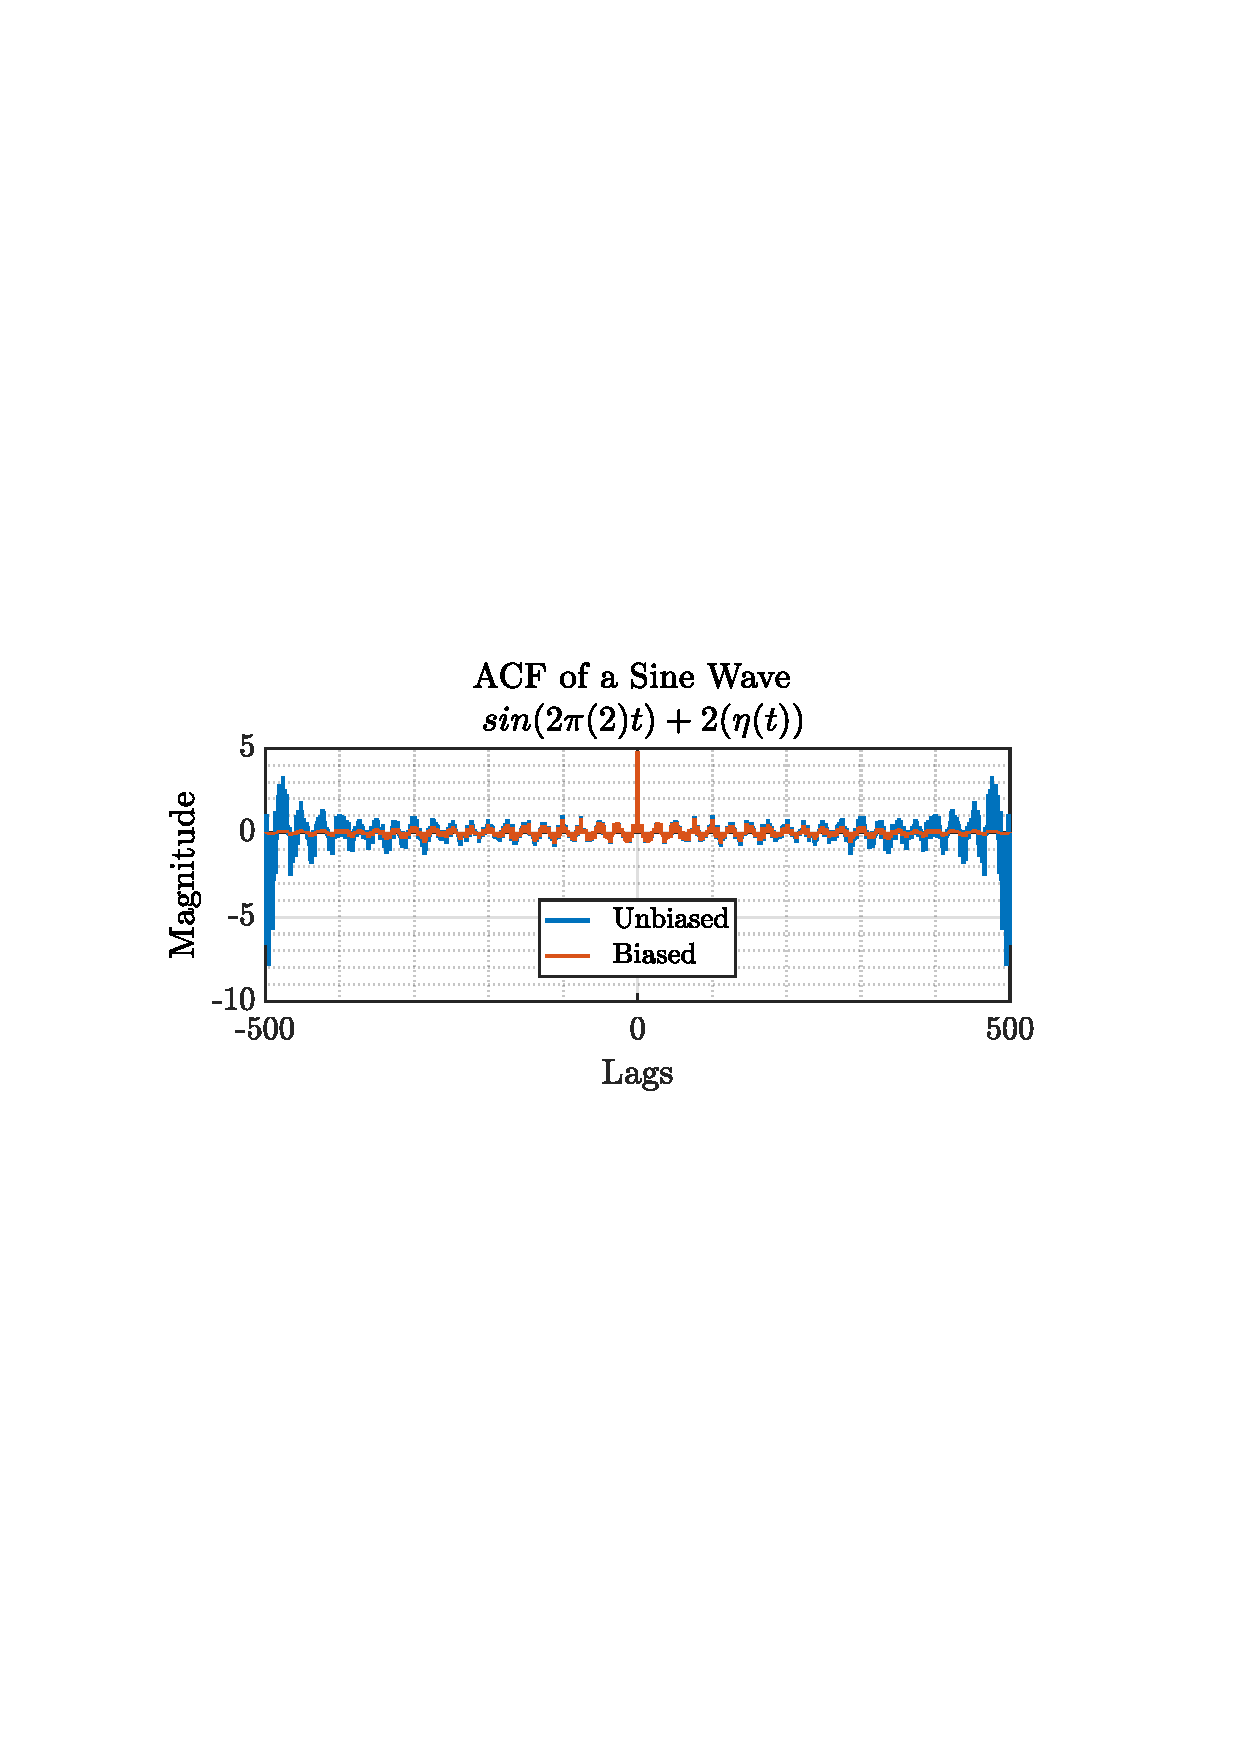
\includegraphics[trim={2.2cm 11.2cm 3.15cm  11.2cm}, clip, width=\textwidth]{../MATLAB/figures/q1_1b_fig01.pdf} 
		\captionsetup{justification=centering}
		\caption{An example of the Limiting Case of the Periodogram Definition}
		\label{fig: 1-1b}
	\end{figure}
	
	
	\subsection{Periodogram-based Methods Applied to Real–World Data} \label{sec: 1-2-PSD-real-world}
	\subsubsection{The SunSpot Dataset}
	Figure \ref{fig: 1-2a}. The mean's influence on data is the offset DC bias, captured in the $f=0$ component of the periodogram. Hence as we would expect, subtracting the \texttt{mean} reduces its magnitude in the periodogram. \texttt{detrend} removes linear trends, it seems in the case of this data set that most linear trends are captured at $f \lessapprox 0.02 rad/sample$. \\
	
	The natural logarithm was taken using: \texttt{log}. As the logarithm has a compression effect on magnitude we see that the magnitude of both raw and periodogram is greatly attenuated. We note that frequencies of interest and its harmonics appear as more distinct when compared to the rest of the periodogram.

	\begin{figure}[H]
		\centering
		\begin{subfigure}{0.49\textwidth}
			\centering
			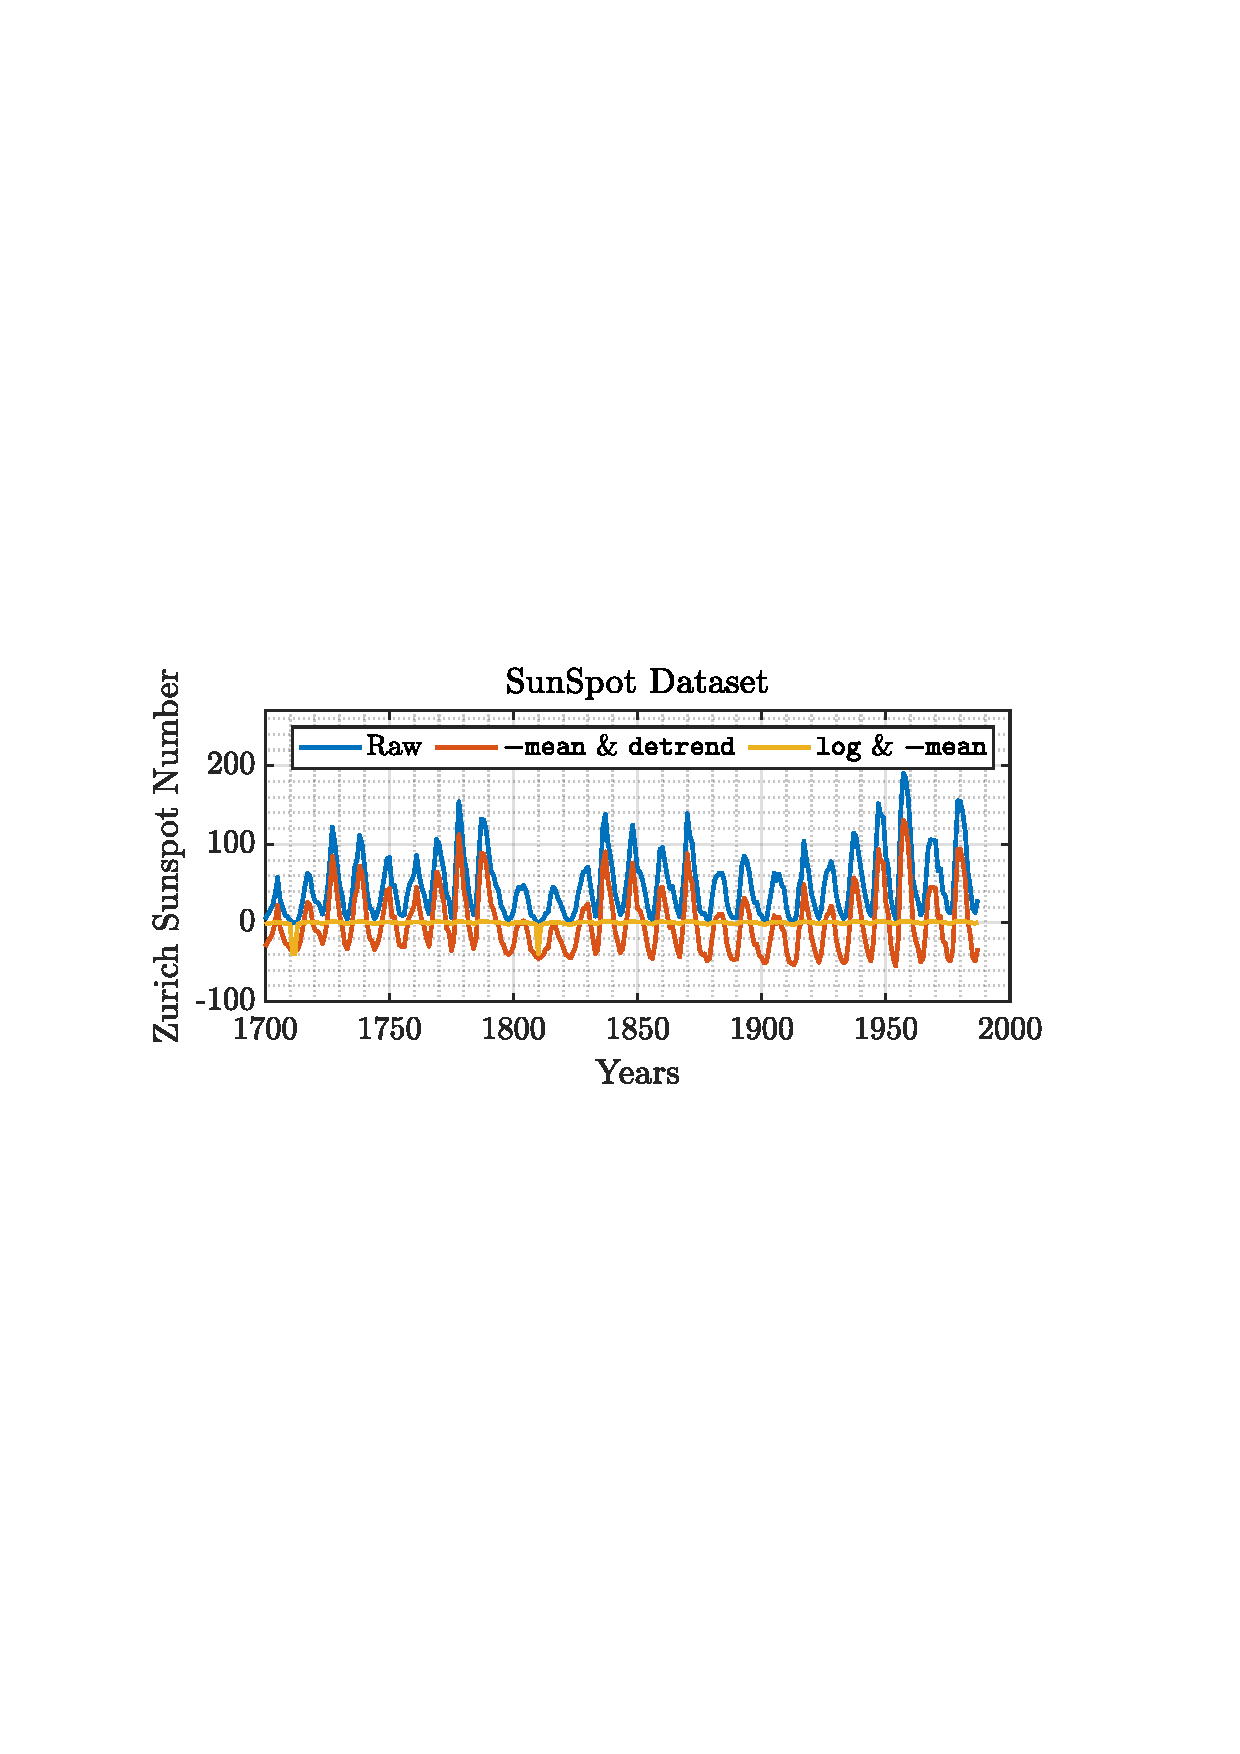
\includegraphics[trim={2.2cm 11.2cm 3.15cm  11.2cm}, clip, width=\textwidth]{../MATLAB/figures/q1_2a_fig01.pdf} 
			\captionsetup{justification=centering}
			\caption{Raw and its preprocessed datas}
		\end{subfigure}
%		~ % forces onto the same row
		\begin{subfigure}{0.49\textwidth}
			\centering
			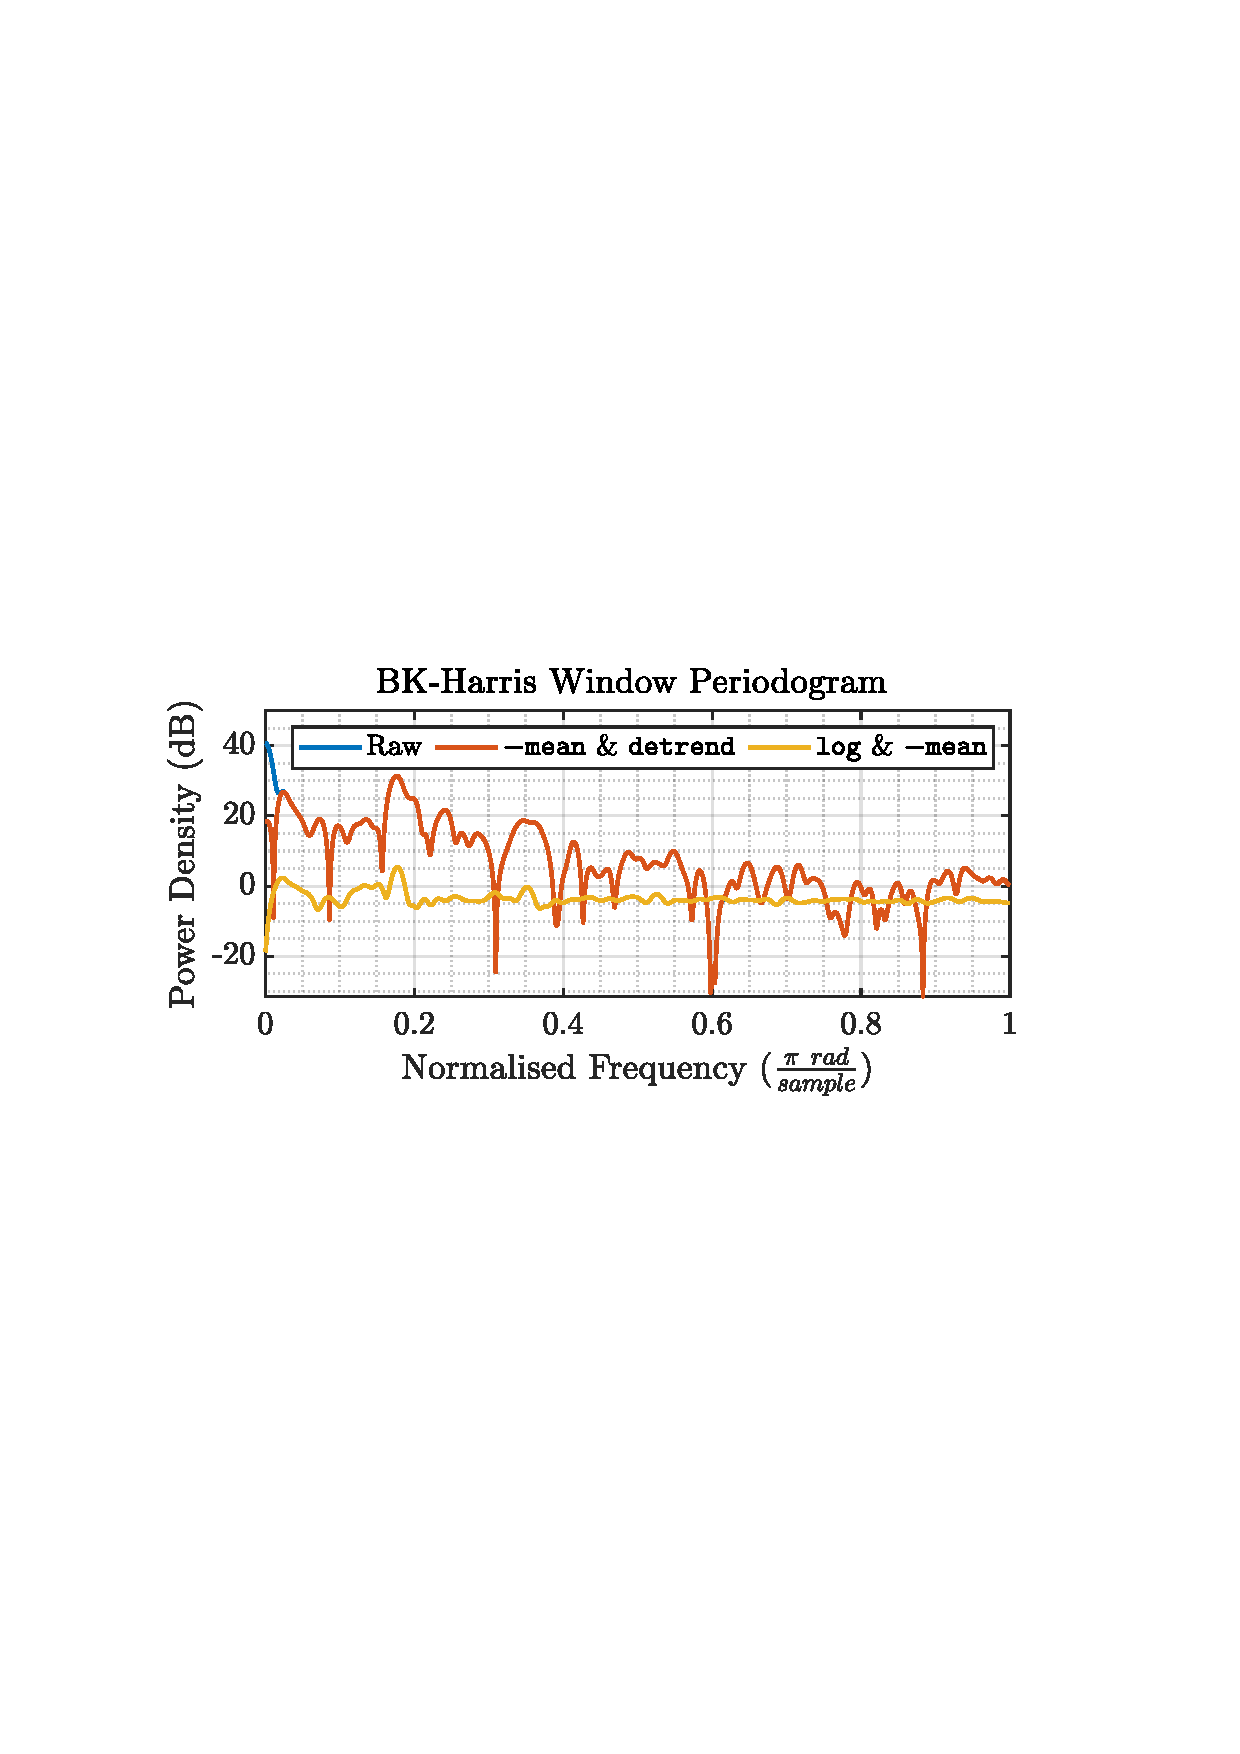
\includegraphics[trim={2.2cm 11.2cm 3.15cm  11.2cm}, clip, width=\textwidth]{../MATLAB/figures/q1_2a_fig02.pdf} 
			\captionsetup{justification=centering}
			\caption{Periodograms}
		\end{subfigure}
		\captionsetup{justification=centering}
		\caption{}
		\label{fig: 1-2a}
	\end{figure}
%	\begin{figure}[H]
%		\centering
%		%\begin{subfigure}[t]{0.4\textwidth}
%		%	\centering
%		%\hspace*{-2.1cm}
%		% 				trim={<left> <lower> <right> <upper>}
%		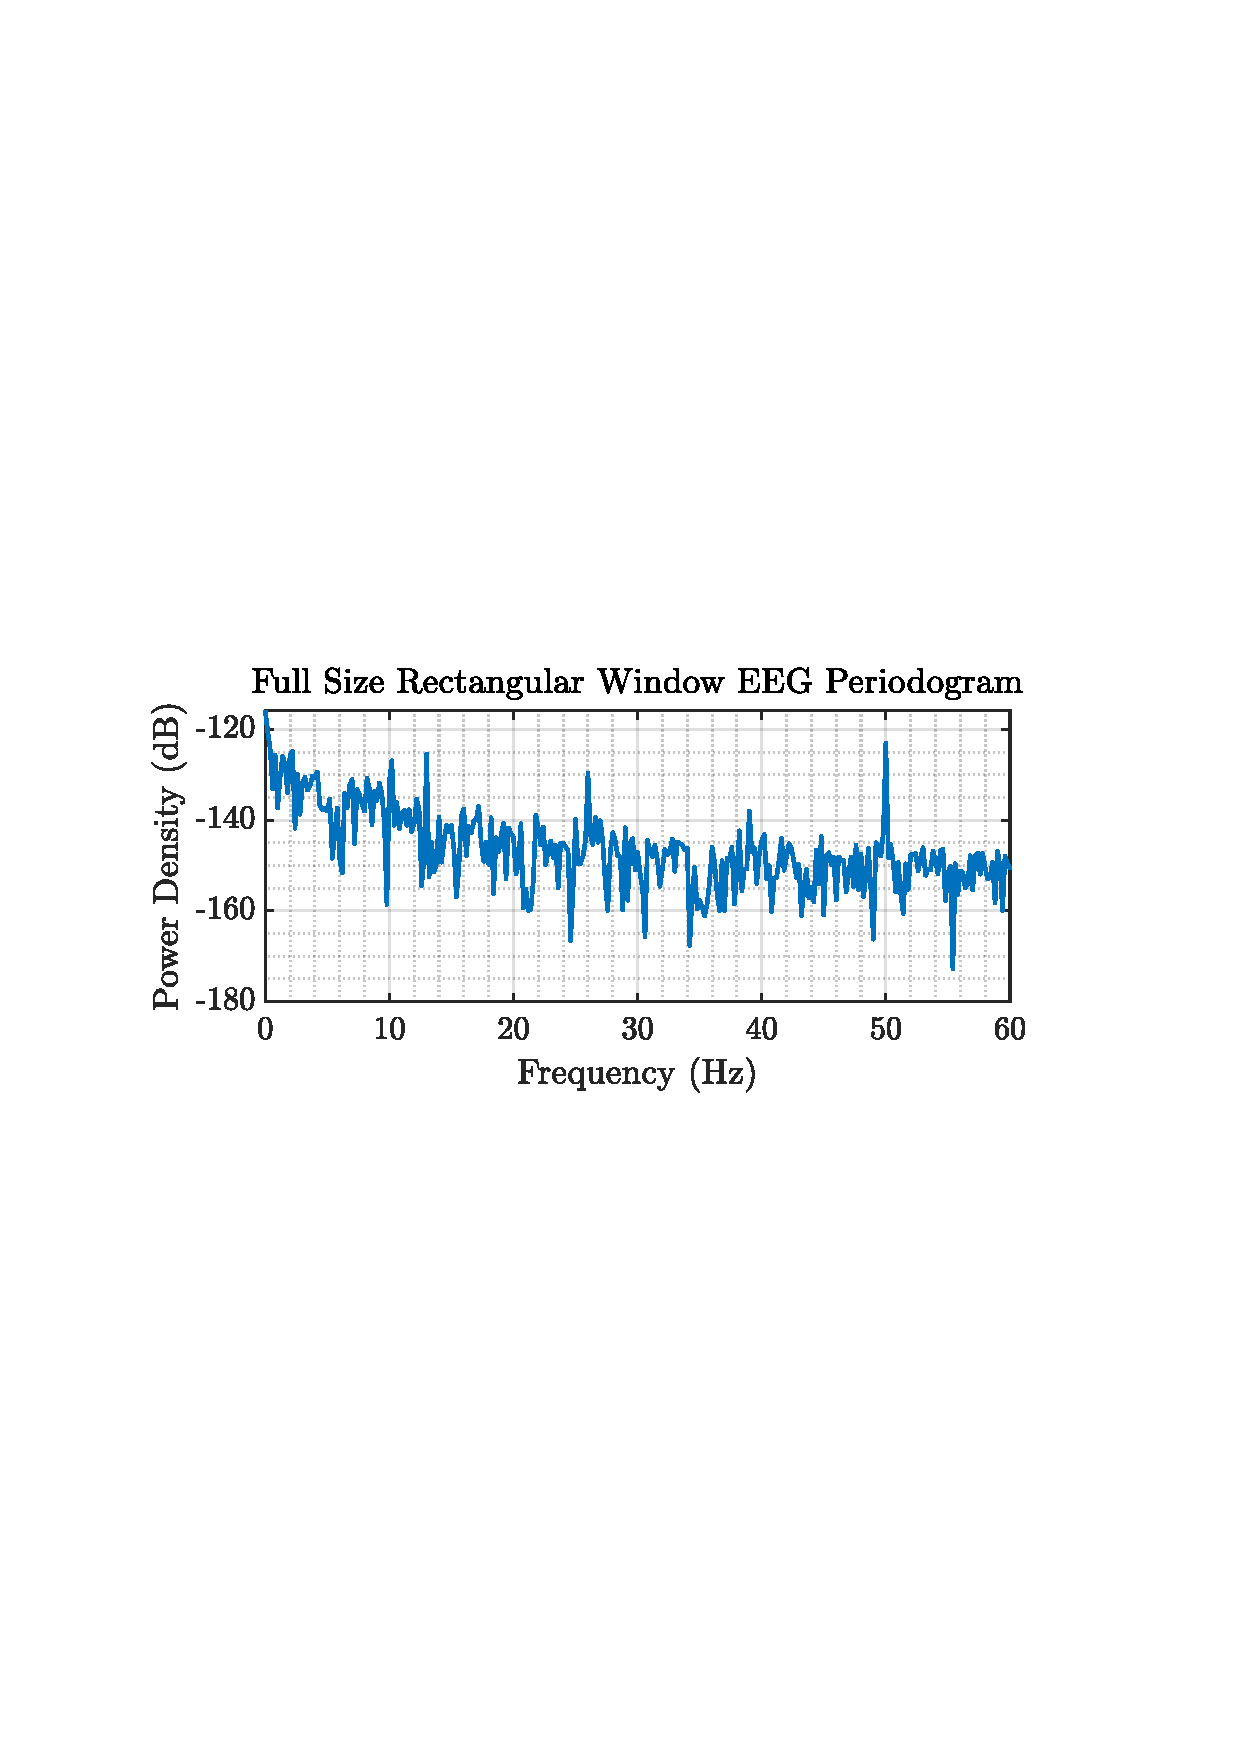
\includegraphics[trim={2.2cm 11.2cm 3.15cm  11.2cm}, clip, width=9cm]{../MATLAB/figures/q1_2b_fig01.pdf} 
%		%	\captionsetup{justification=centering}
%		%	\caption{Vertical gel electrophoresis setup} 
%		%	\label{fig: verticalGel}
%		%\end{subfigure}
%		%\hfill
%		\captionsetup{justification=centering}
%		\caption{Science being done here}
%	\end{figure}


	\subsubsection{The EEG Dataset}
	
	\begin{figure}[H]
		\centering
		\begin{subfigure}{0.49\textwidth}
			\centering
			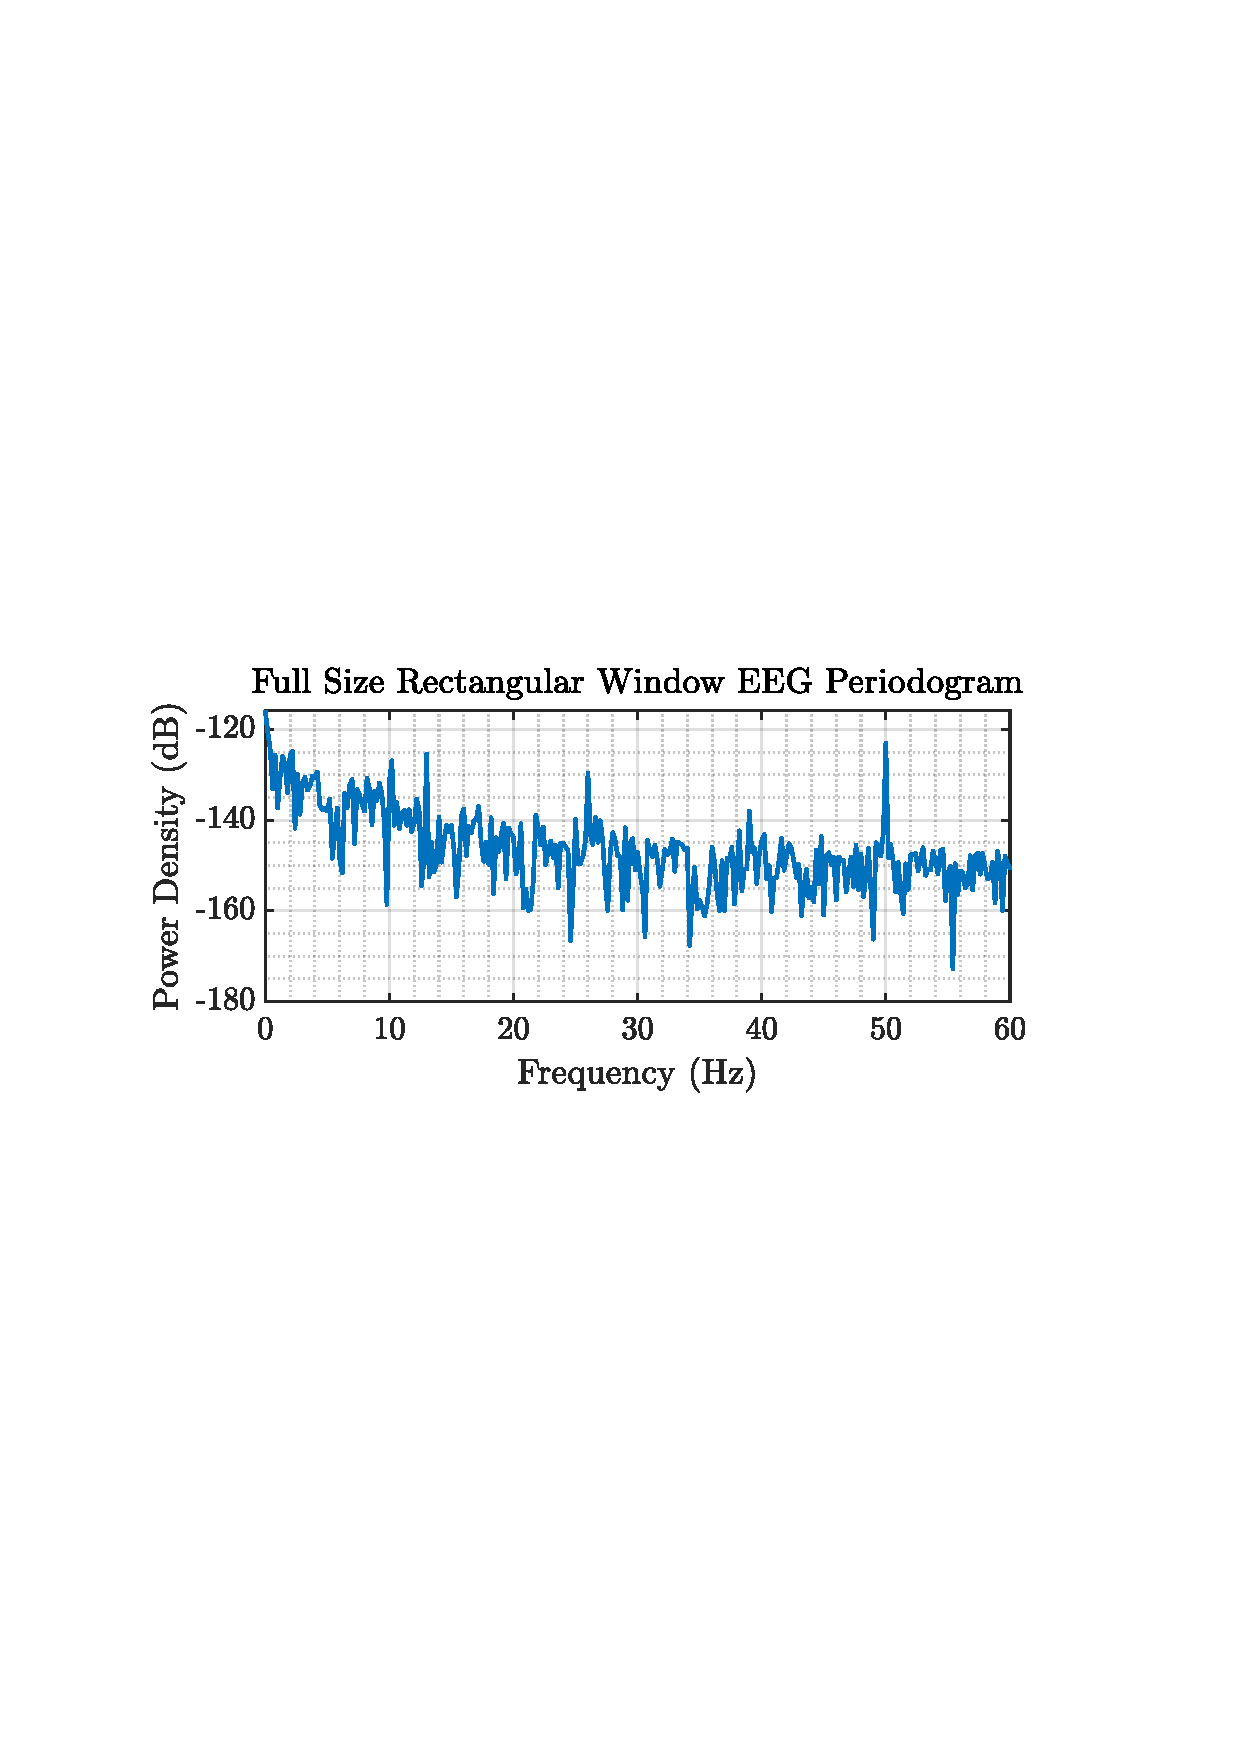
\includegraphics[trim={2.2cm 11.2cm 3.15cm  11.2cm}, clip, width=\textwidth]{../MATLAB/figures/q1_2b_fig01.pdf} 
			\captionsetup{justification=centering}
			\caption{Standard Periodogram}
		\end{subfigure}
		%		~ % forces onto the same row
		\begin{subfigure}{0.49\textwidth}
			\centering
			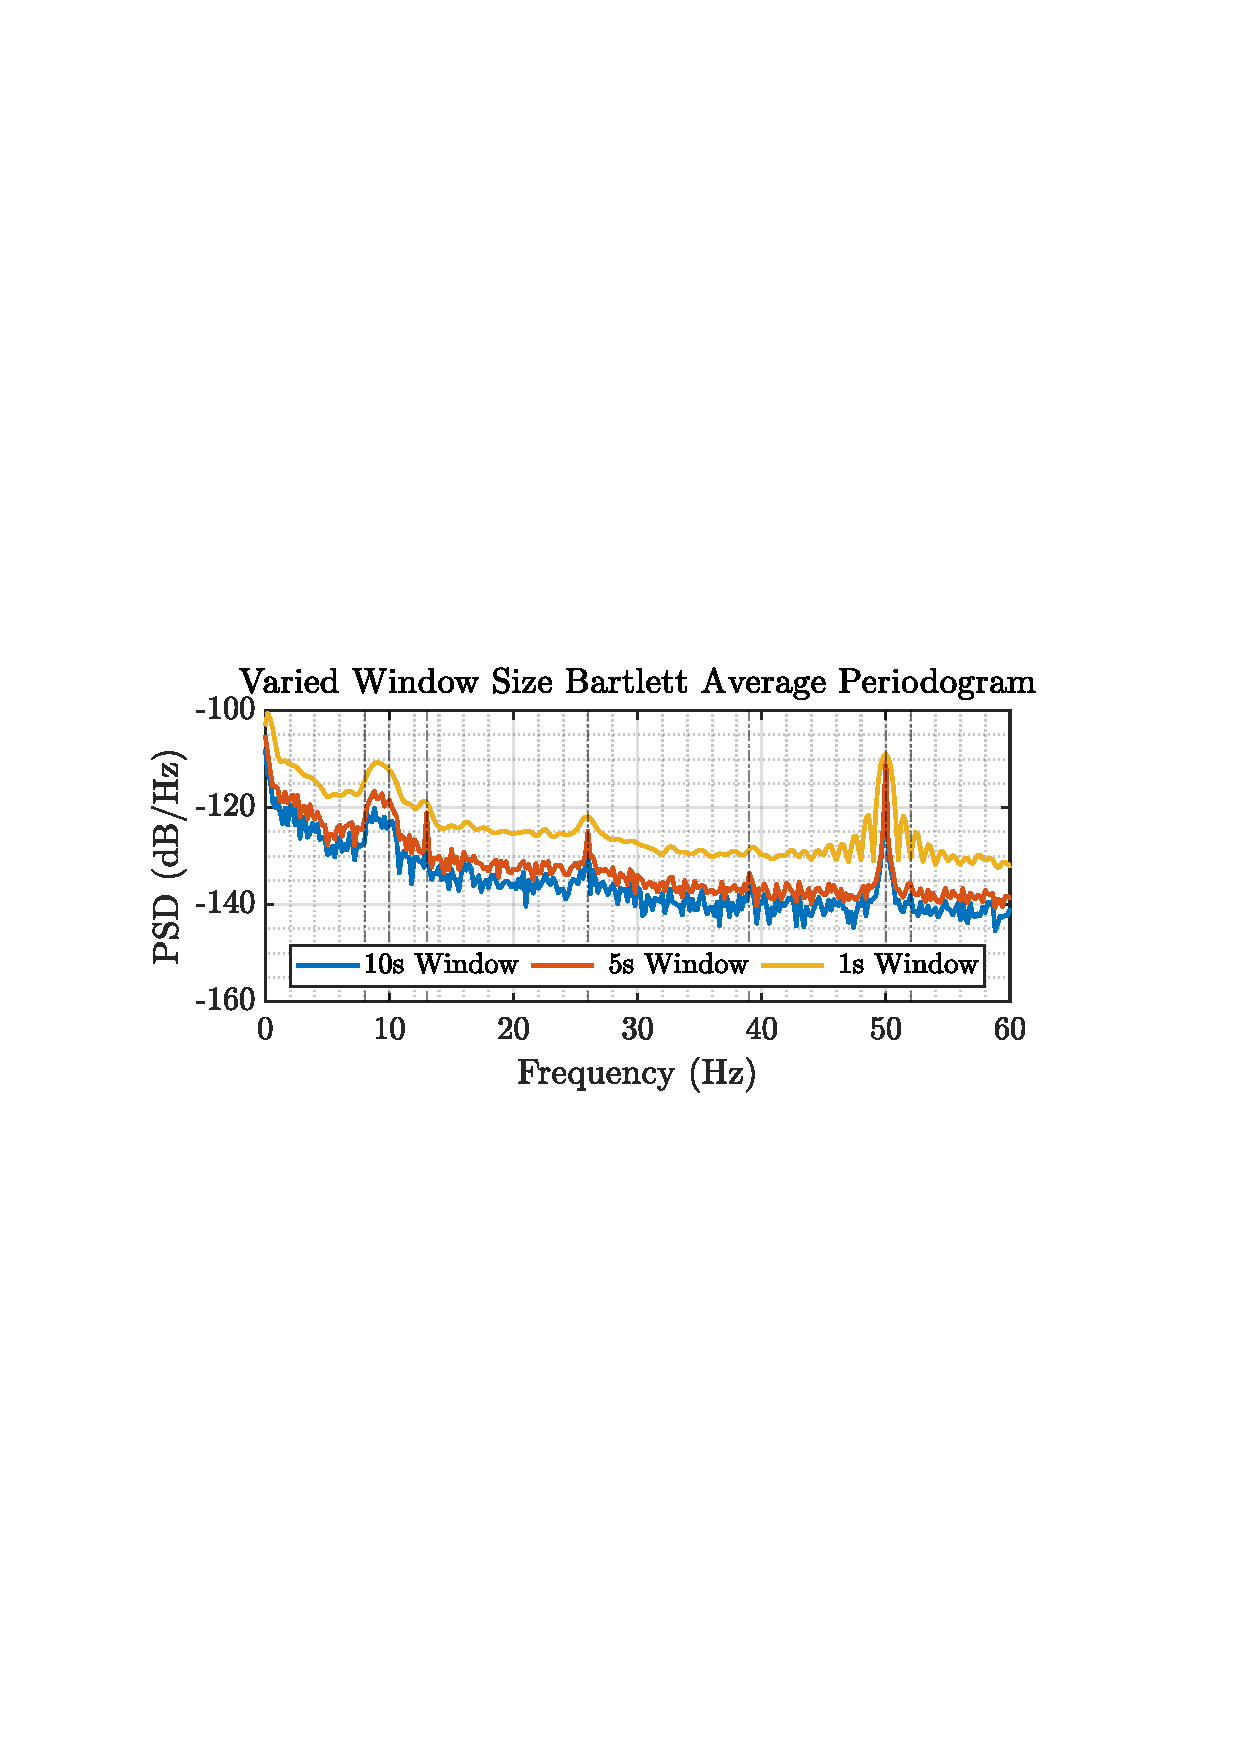
\includegraphics[trim={2.2cm 11.2cm 3.15cm  11.2cm}, clip, width=\textwidth]{../MATLAB/figures/q1_2b_fig02.pdf} 
			\captionsetup{justification=centering}
			\caption{Bartlett Average Periodograms}
		\end{subfigure}
		\captionsetup{justification=centering}
		\caption{}
		\label{fig: 1-2b}
	\end{figure}

	\begin{table}[H]
		\centering
		\begin{tabular}{|c|c||c|}
			\hline
			\textbf{Response} & \textbf{Expected Range} (Hz) & \textbf{Observed Range} (Hz) \\
			\hline
			{Alpha Rhythm} & $8 - 10$ & $8-10$ \\
			\hline
			{SSVEP} & \texttt{range}[$11-20$] & $13n$ \\
			\hline
			{Power-Line} & $50$ & $50$ \\
			\hline
		\end{tabular}
		\captionsetup{justification=centering}
		\caption{EEG Frequency Peaks of the Periodogram. $n$ refers to harmonics}
		\label{tab: 1-2b}
	\end{table}
	
	The standard periodogram has identifiable peaks, showing in Figure \ref{fig: 1-2b}, quantified in Table \ref{tab: 1-2b}. We are unable to identify the 3rd harmonic of the SSVEP, at 52Hz it is too close to the power-line interference at 50Hz. The main difference in the 10s window averaged periodogram is clearer peak isolation compared to the surrounding periodogram and emphasis on the range of frequencies of the alpha-rhythm, rather than a single discrete peak.

	\subsection{Correlation Estimation} \label{sec: 1-3-correlation-est}
	
	\subsubsection{Unbiased and Biased ACF Estimates}
	
	\begin{figure}[H]
		\centering
		\begin{subfigure}{0.49\textwidth}
			\centering
			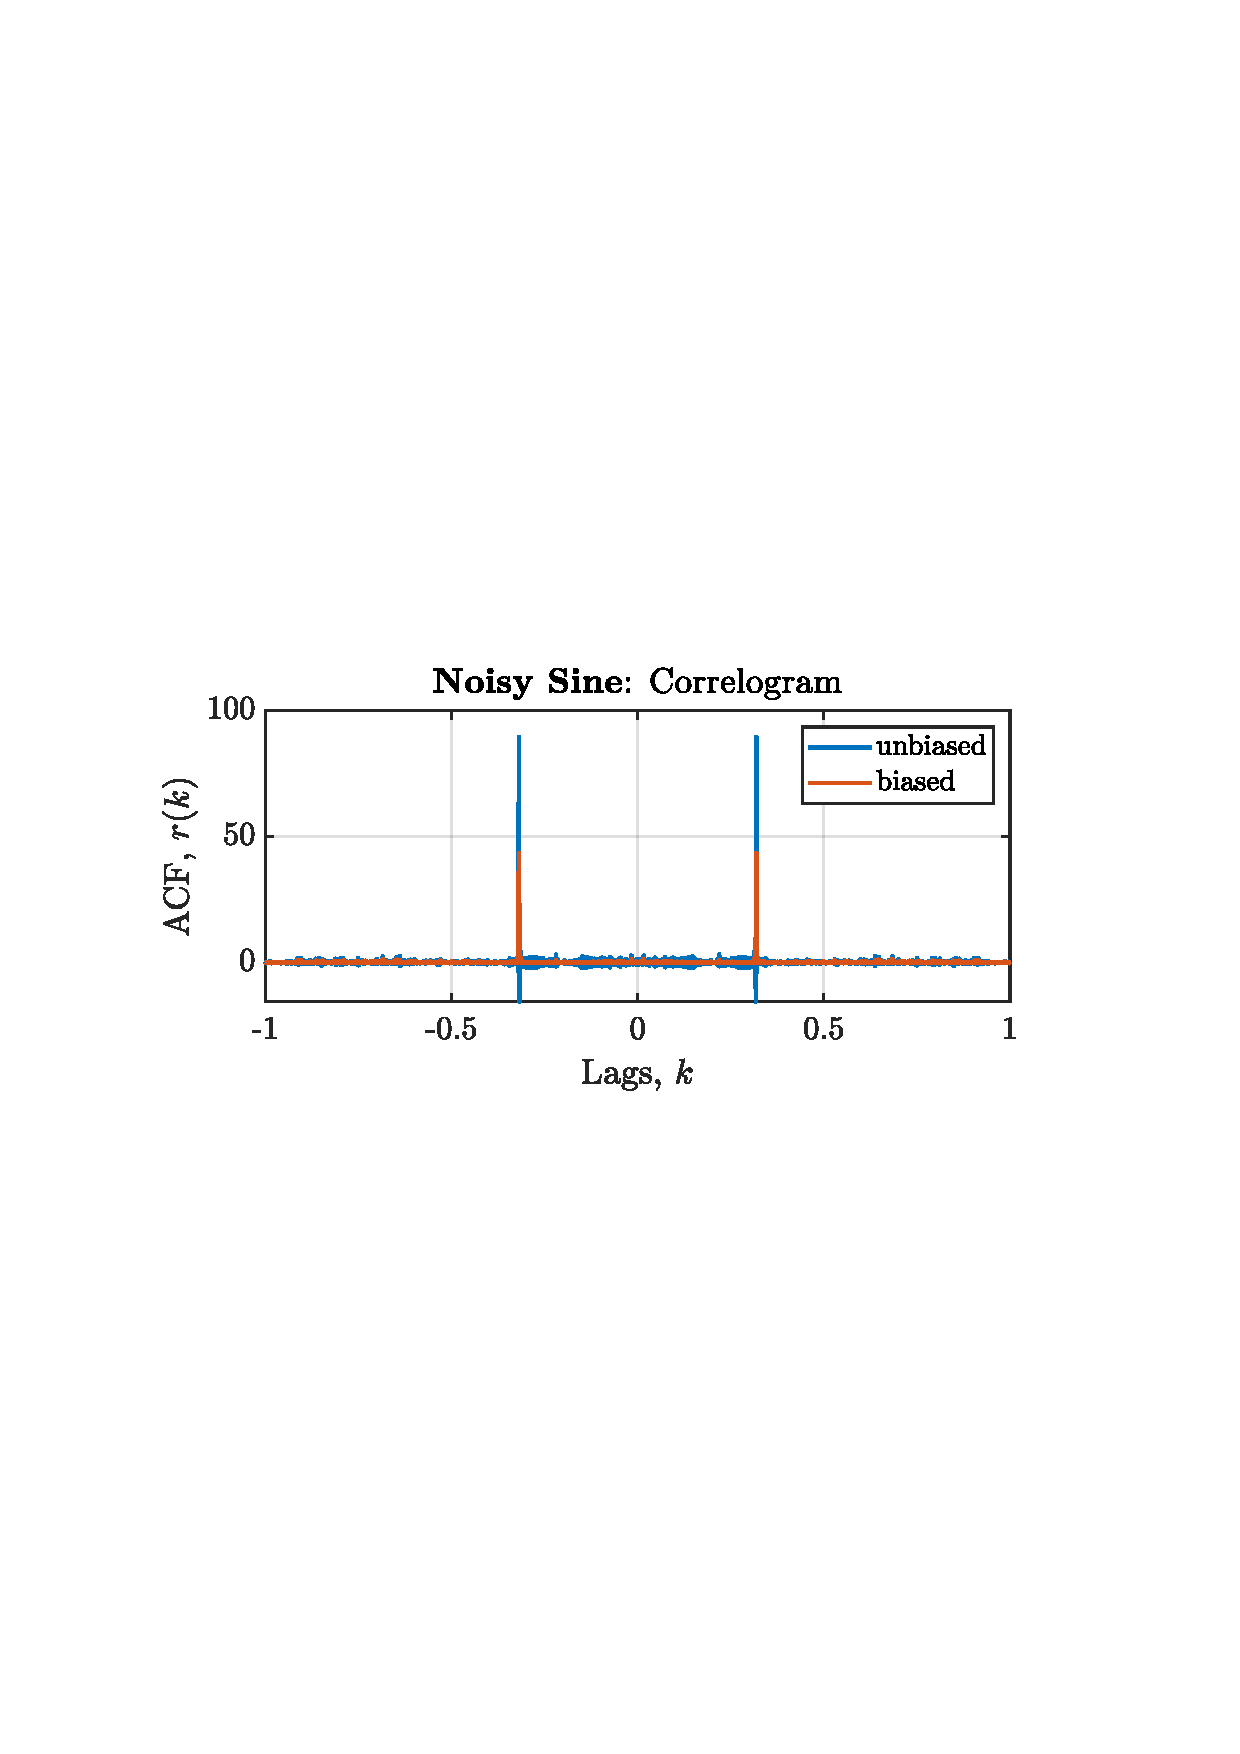
\includegraphics[trim={2.2cm 11cm 3.15cm  11.2cm}, clip, width=\textwidth]{../MATLAB/figures/q1_3a_fig04.pdf} 
		\end{subfigure}
		%		~ % forces onto the same row
		\begin{subfigure}{0.49\textwidth}
			\centering
			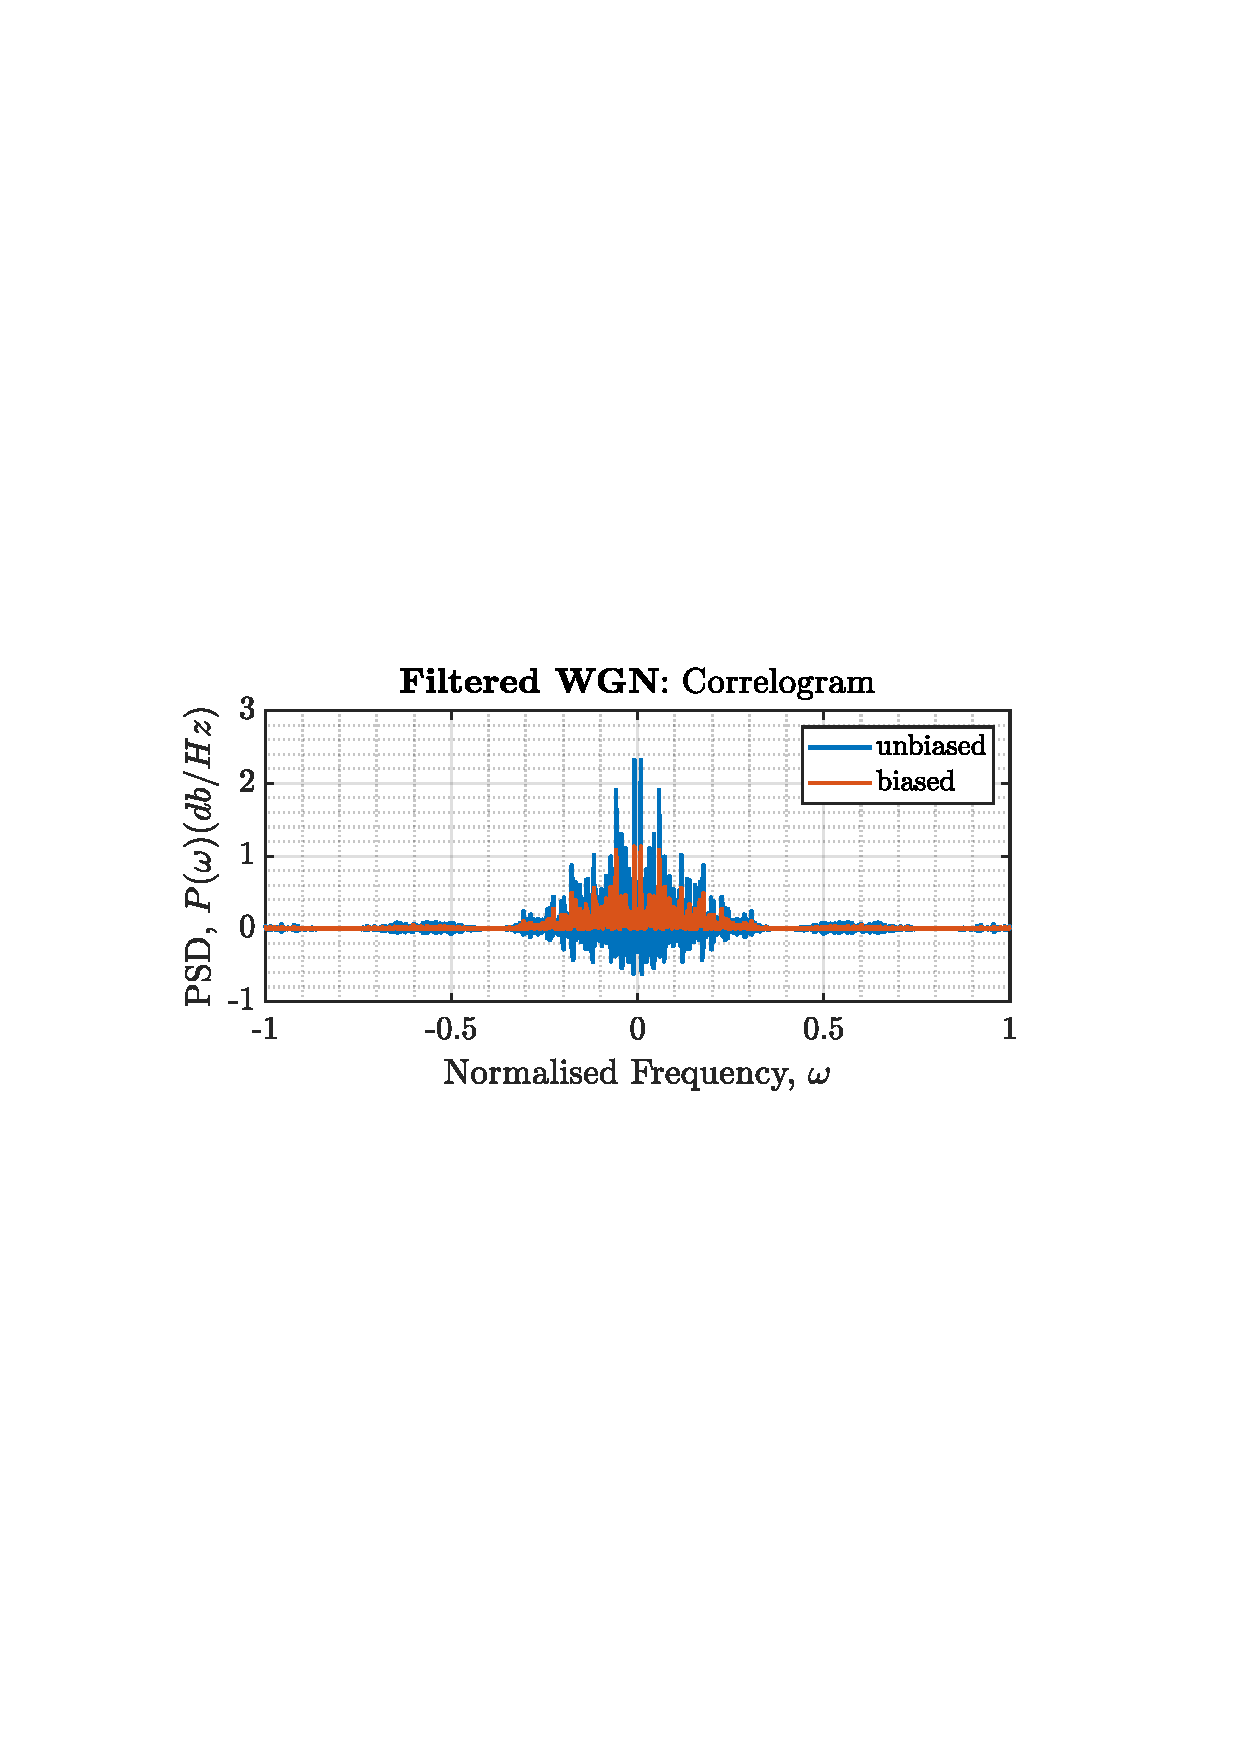
\includegraphics[trim={2.2cm 11cm 3.15cm  11.2cm}, clip, width=\textwidth]{../MATLAB/figures/q1_3a_fig05.pdf} 
		\end{subfigure}
				\begin{subfigure}{0.49\textwidth}
			\centering
			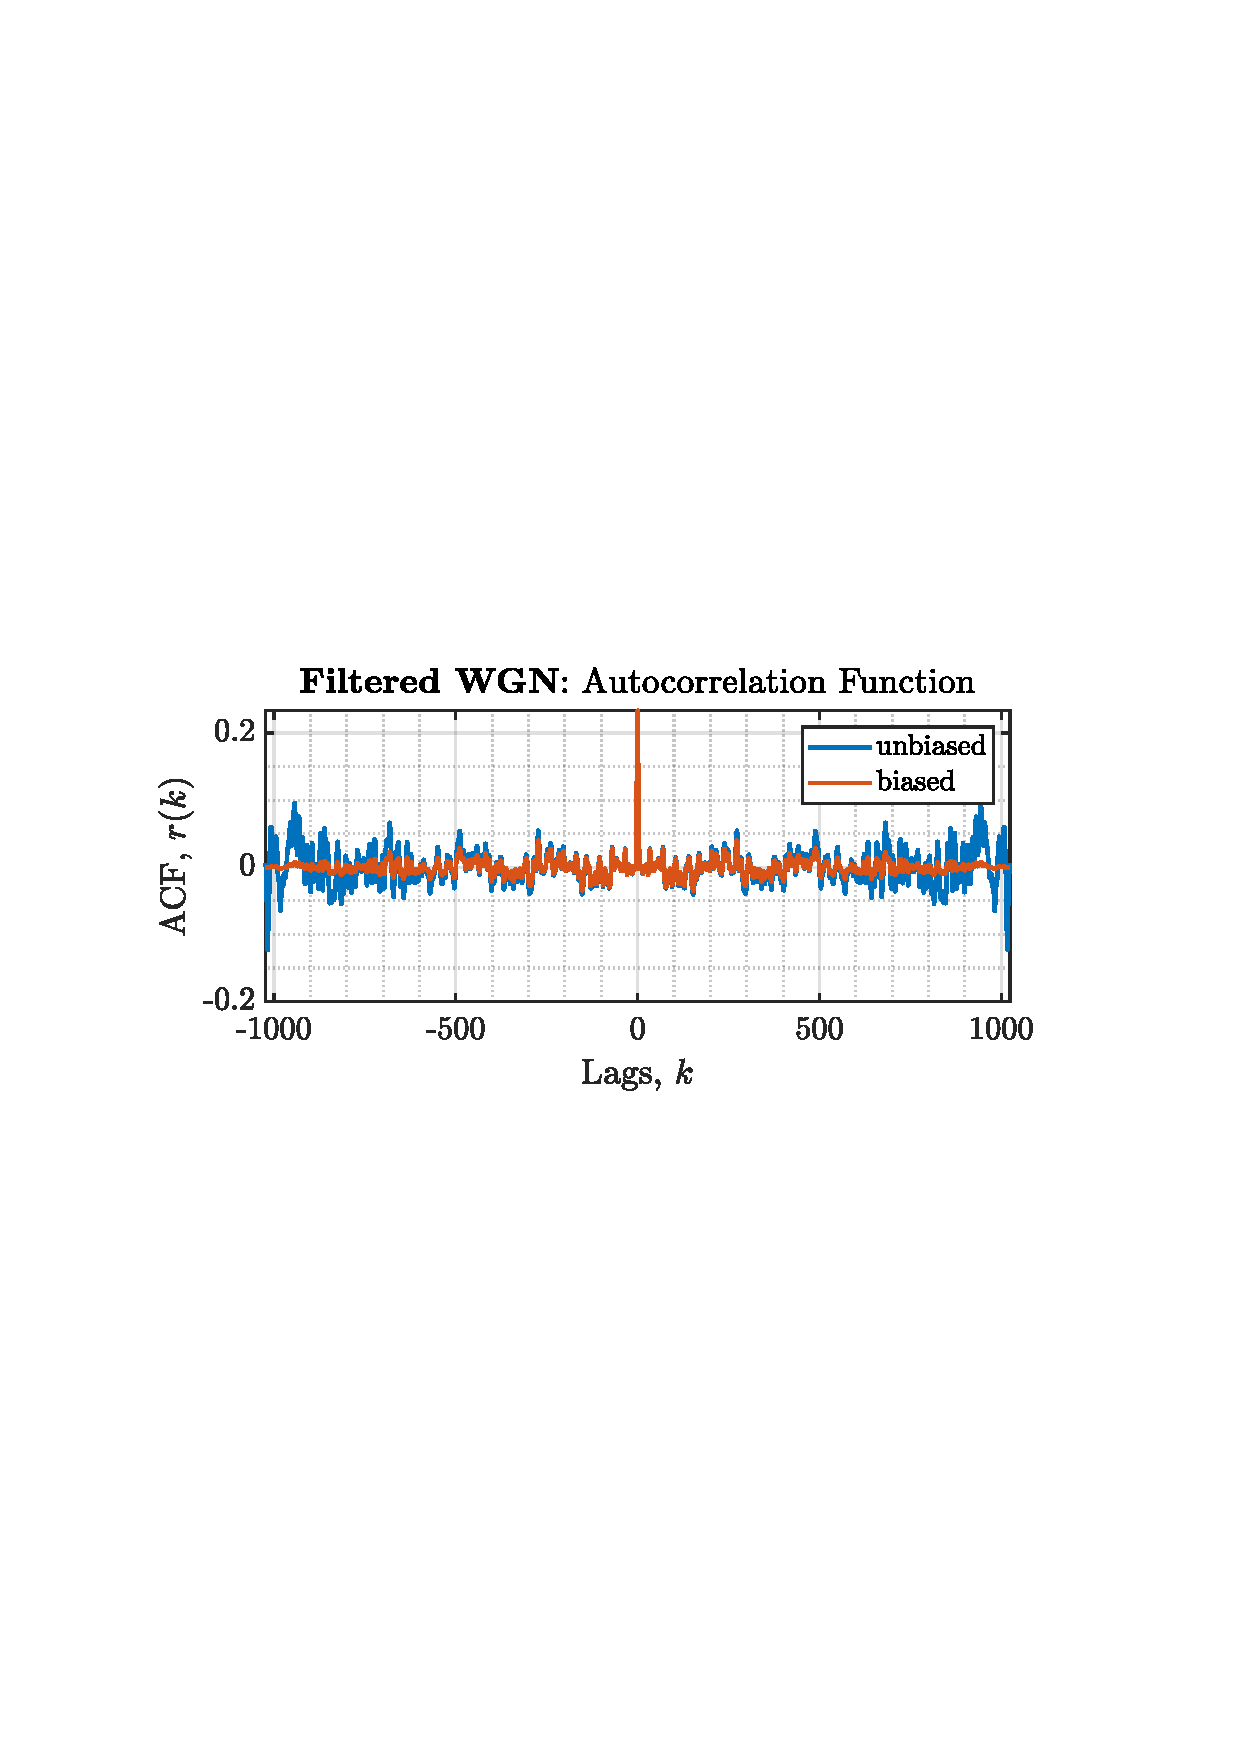
\includegraphics[trim={2.2cm 11cm 3.15cm  11.2cm}, clip, width=\textwidth]{../MATLAB/figures/q1_3a_fig06.pdf} 
		\end{subfigure}
		%		~ % forces onto the same row
		\begin{subfigure}{0.49\textwidth}
			\centering
			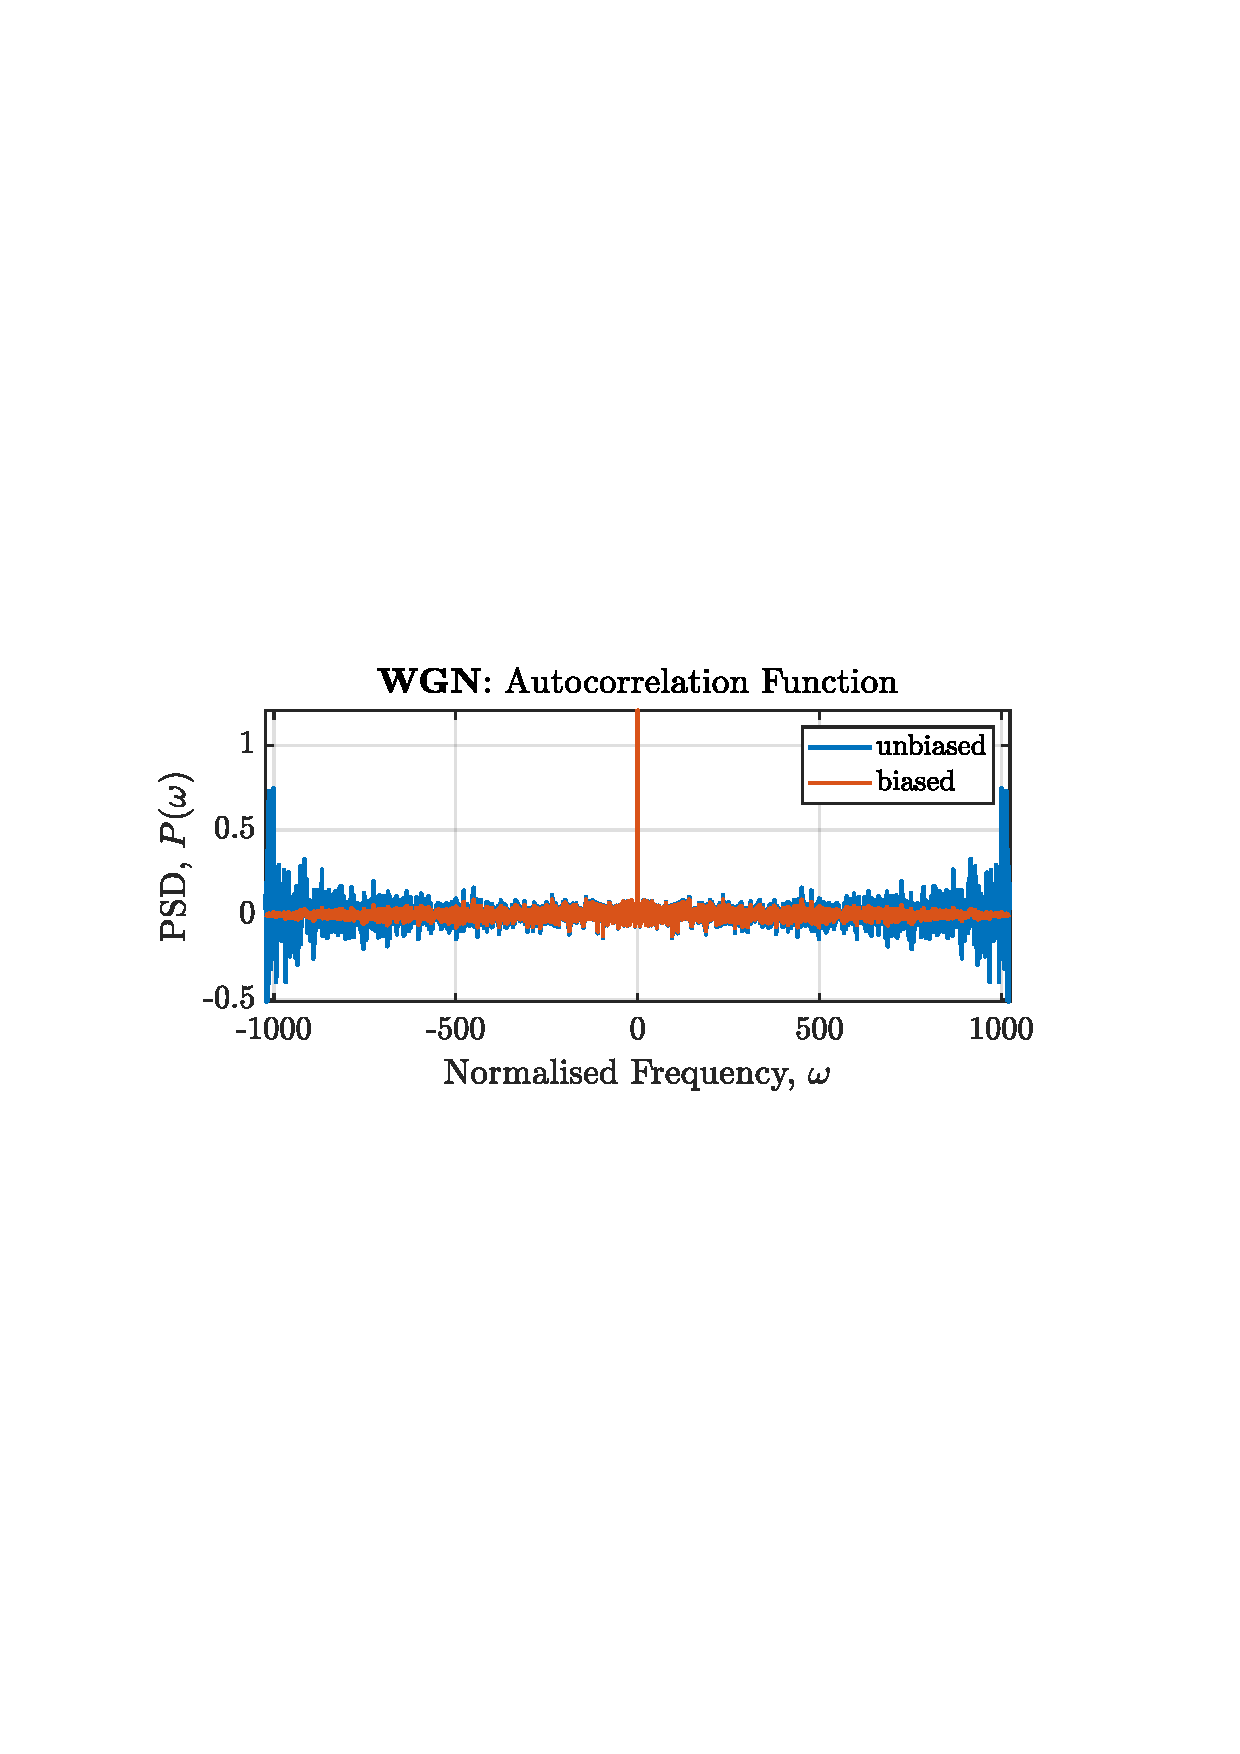
\includegraphics[trim={2.2cm 11cm 3.15cm  11.2cm}, clip, width=\textwidth]{../MATLAB/figures/q1_3a_fig01.pdf} 
		\end{subfigure}
		\begin{subfigure}{0.49\textwidth}
			\centering
			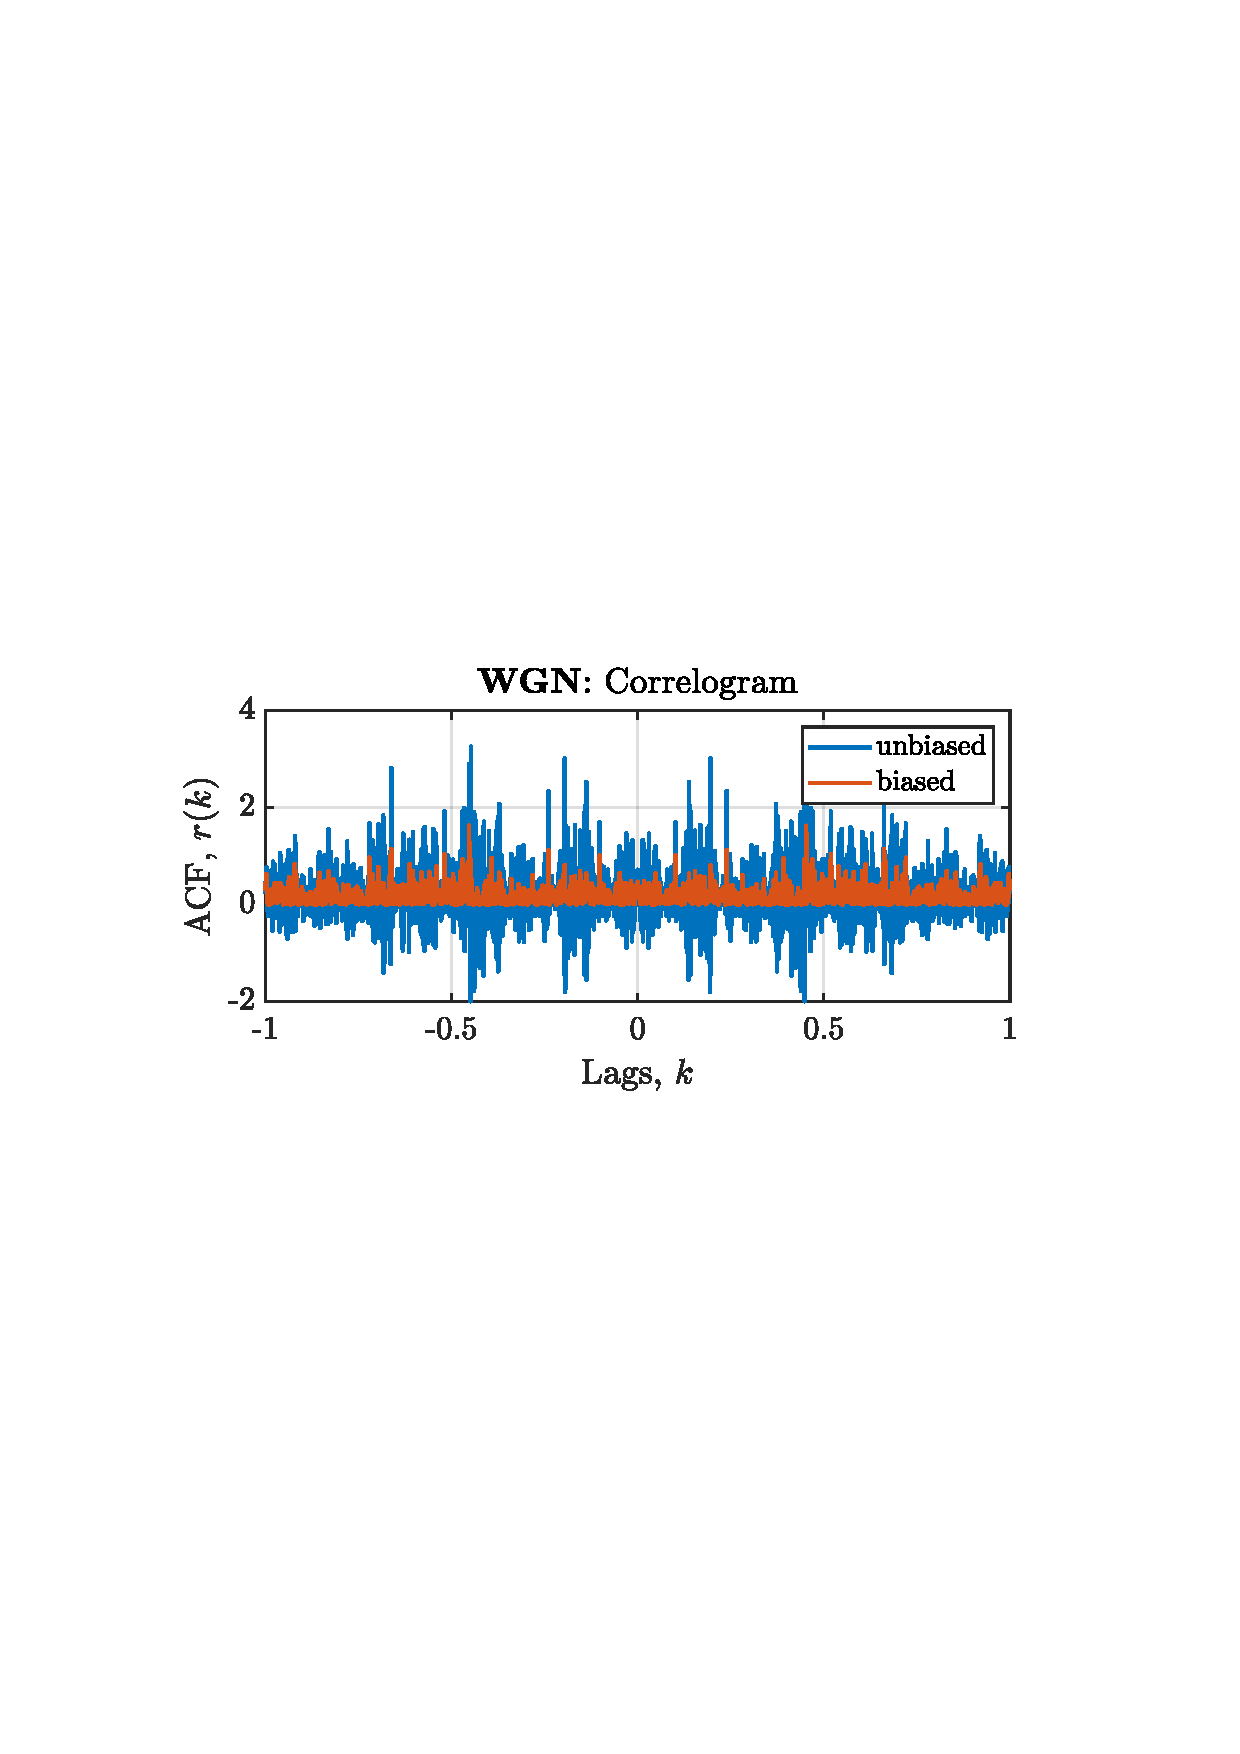
\includegraphics[trim={2.2cm 11.2cm 3.15cm  11.2cm}, clip, width=\textwidth]{../MATLAB/figures/q1_3a_fig02.pdf} 
		\end{subfigure}
		%		~ % forces onto the same row
		\begin{subfigure}{0.49\textwidth}
			\centering
			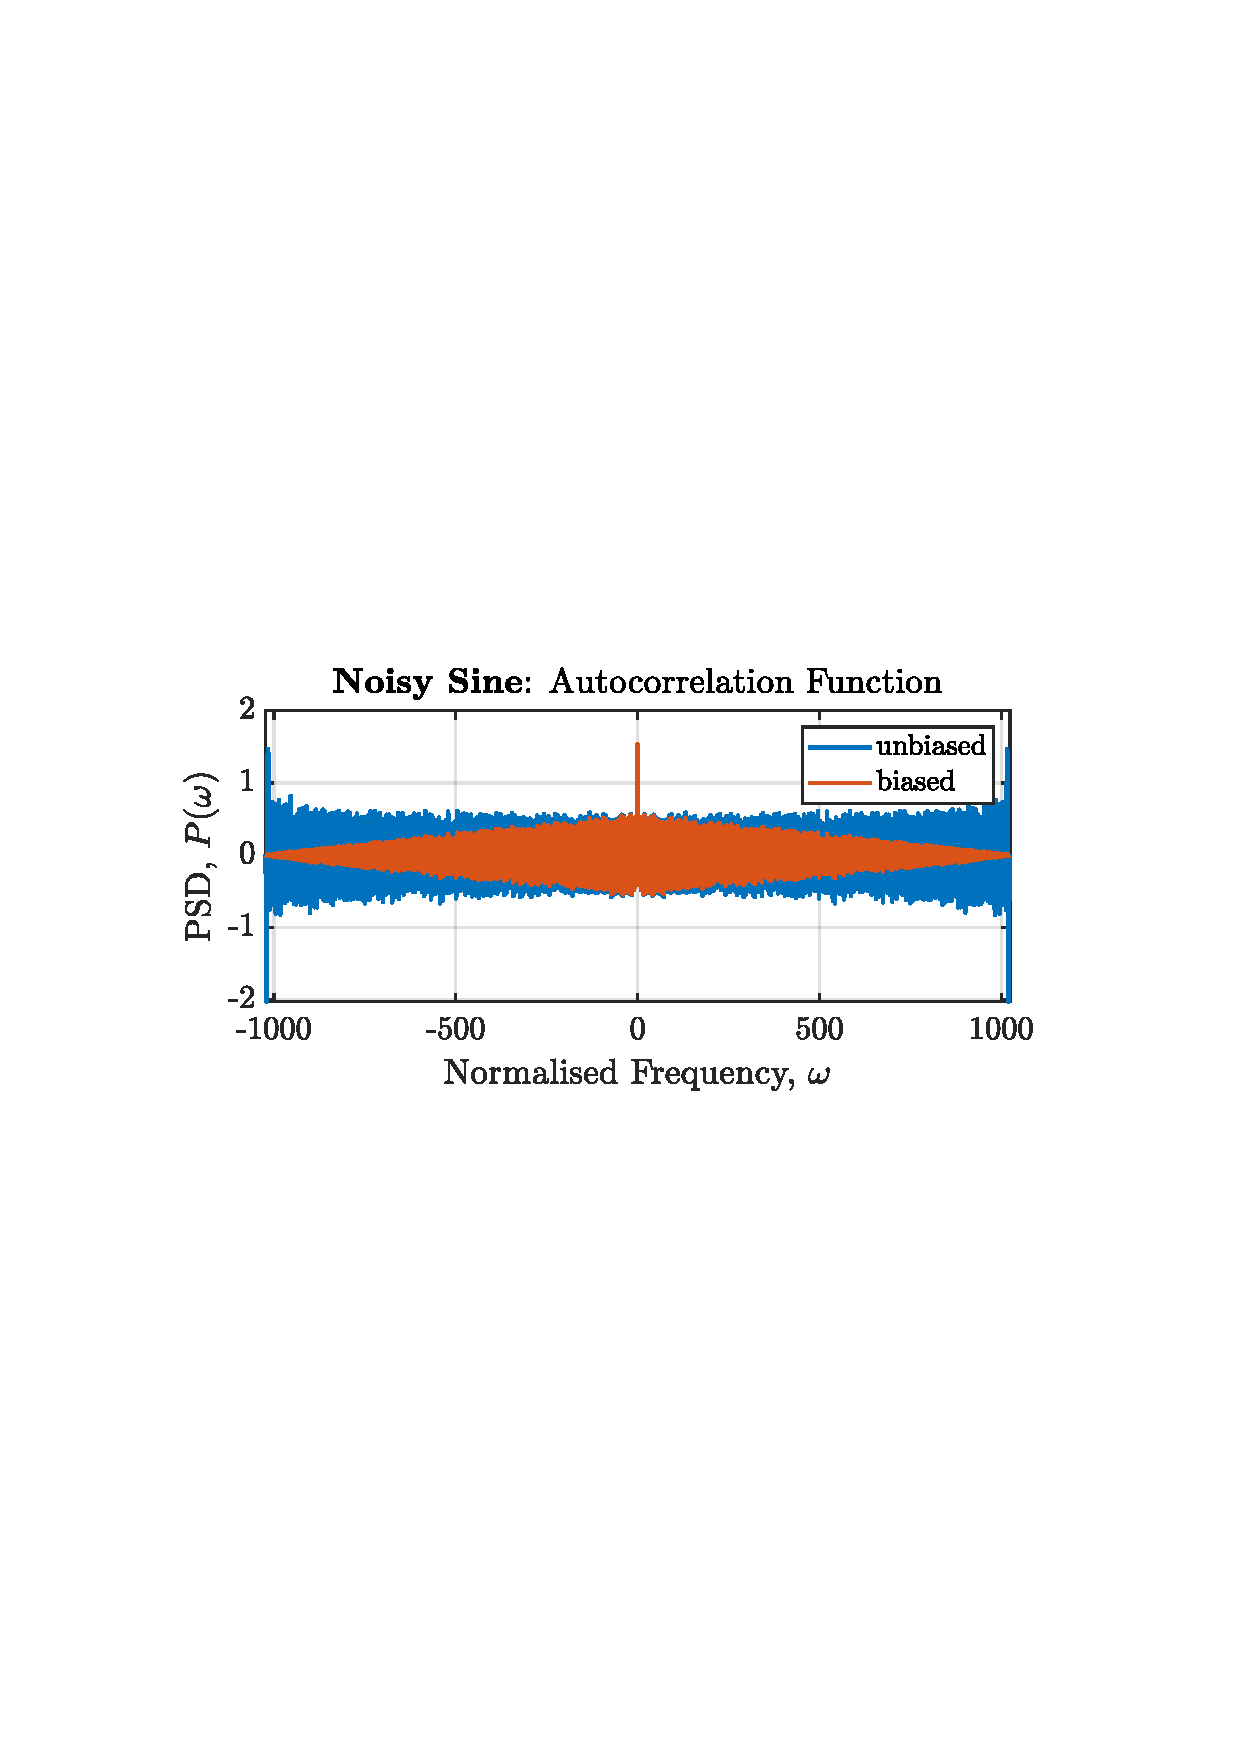
\includegraphics[trim={2.2cm 11.2cm 3.15cm  11.2cm}, clip, width=\textwidth]{../MATLAB/figures/q1_3a_fig03.pdf} 
		\end{subfigure}
		\captionsetup{justification=centering}
		\caption{Set of Auto-Correlation Functions (ACFs) and their Correlograms}
		\label{fig: 1-3a}
	\end{figure}
	
	Figure \ref{fig: 1-3a}. For the autocorrelation functions: we can see that the biased estimator tends to 0 for increasing lag magnitude, whereas the unbiased estimator remains somewhat constant, although at the extremes it begins to increase to approximately double the constant value.\\
	For the correlograms: we observe that the biased estimator does not contain negative values.
	
	\subsubsection{Biased ACF Estimator PSDs}

	The process simulated was the following:
	
	\begin{equation}
		\begin{aligned}
		x(n) = & 2 sin(2 \pi 0.4 n) + 1.75 sin(2 \pi 0.6 n) \\
		&  + 0.85 sin(2 \pi 0.85 n) + 1.2 sin(2 \pi 0.95 n) + \eta(n) \quad \eta \sim \mathcal{N}(0, 1)
		\end{aligned}
	\end{equation}
	
	

	\begin{figure}[H]
		\centering
		\begin{subfigure}{0.49\textwidth}
			\centering
			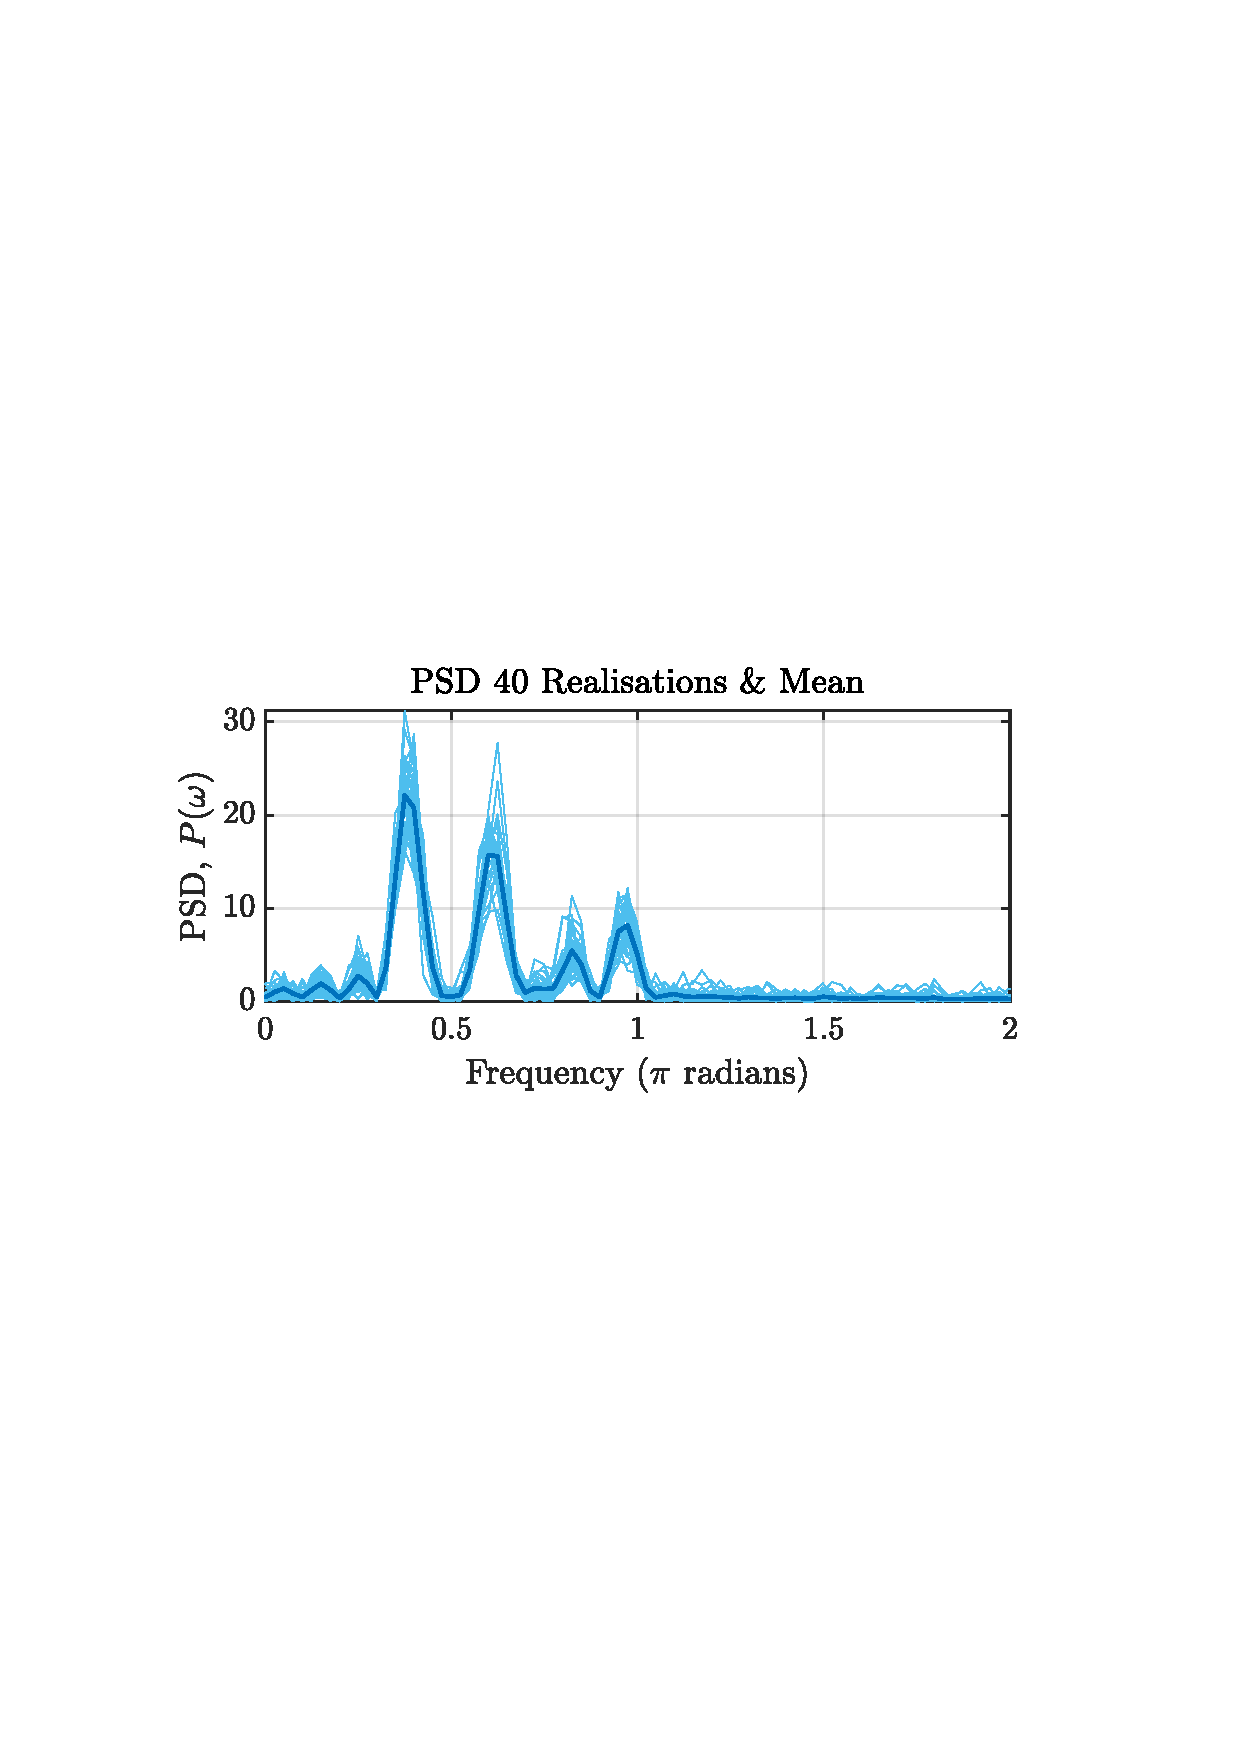
\includegraphics[trim={2.2cm 11.2cm 3.15cm  11.2cm}, clip, width=\textwidth]{../MATLAB/figures/q1_3b_fig01.pdf} 
			\captionsetup{justification=centering}
			\caption{Periodogram}
		\end{subfigure}
		%		~ % forces onto the same row
		\begin{subfigure}{0.49\textwidth}
			\centering
			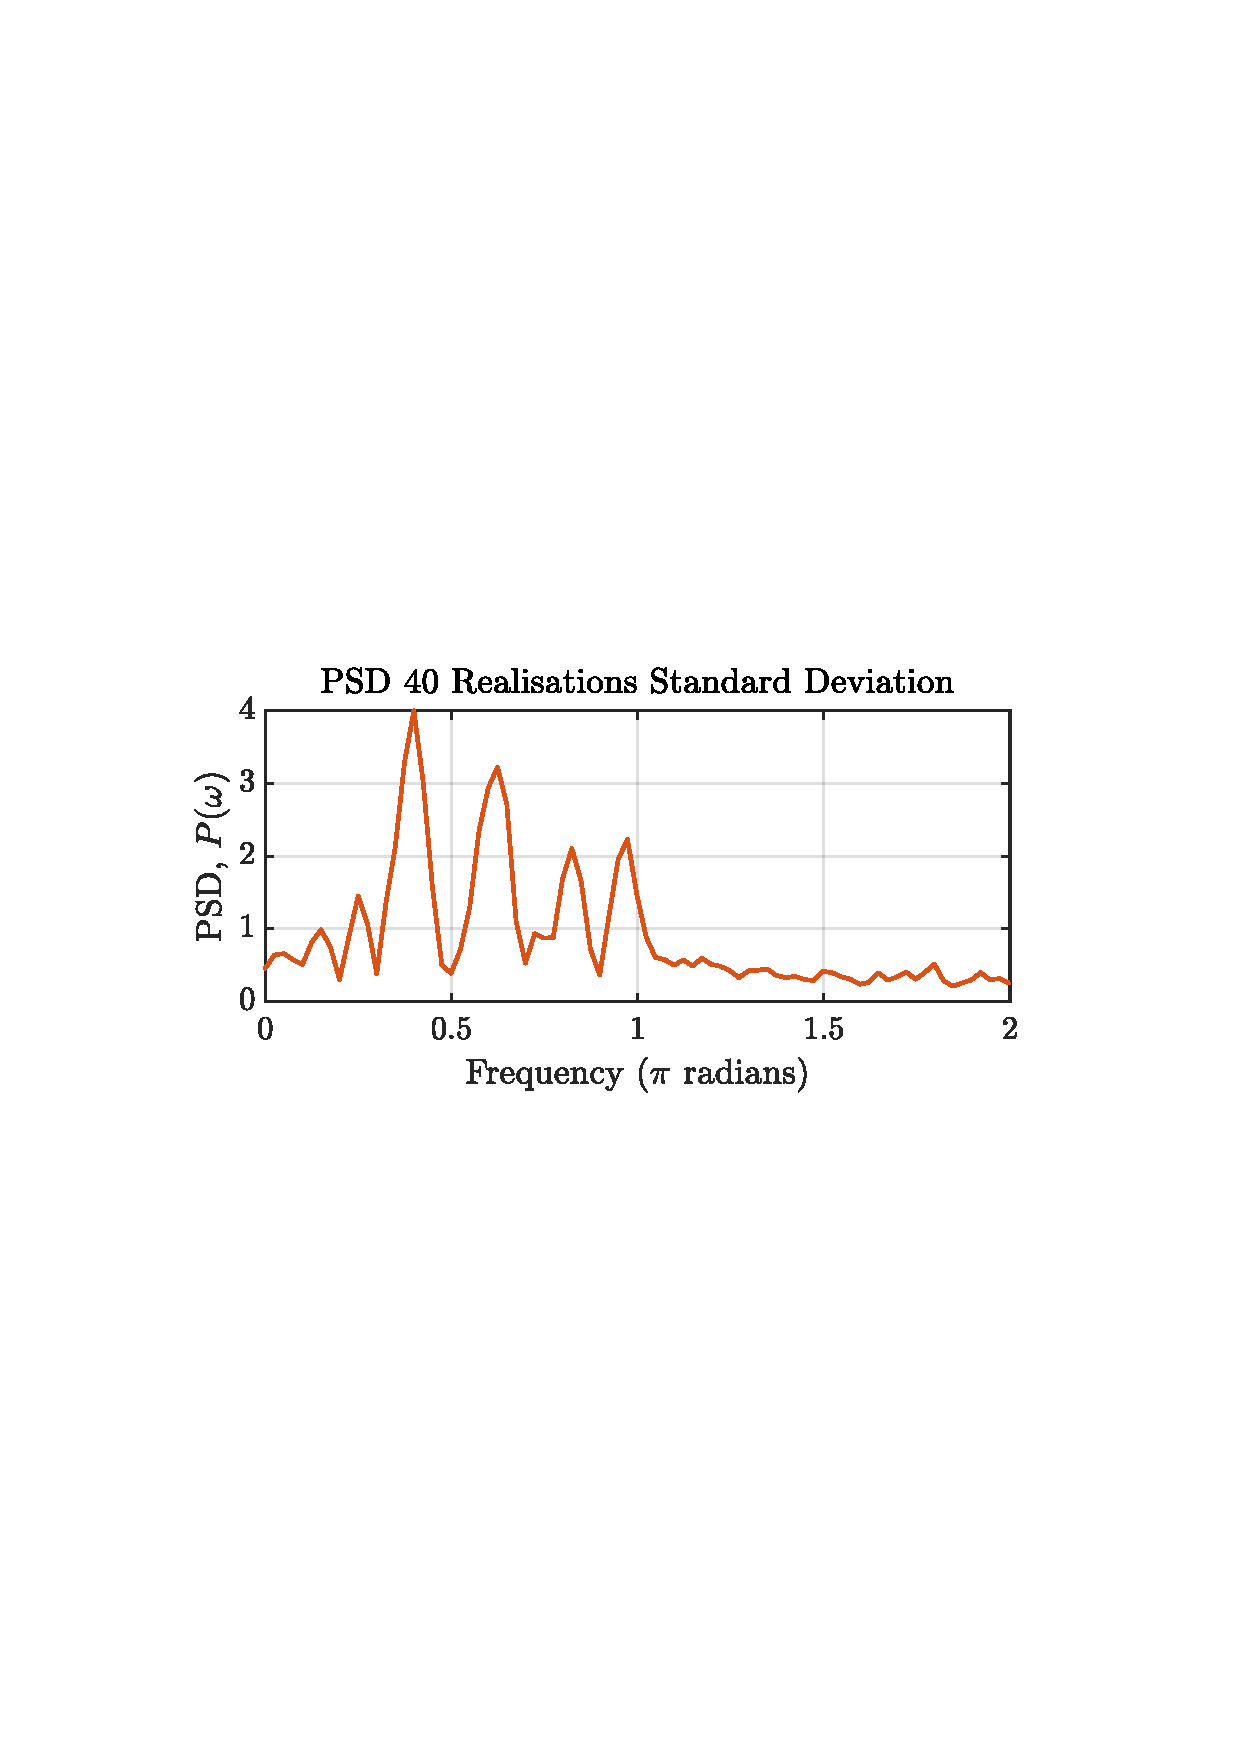
\includegraphics[trim={2.2cm 11.2cm 3.15cm  11.2cm}, clip, width=\textwidth]{../MATLAB/figures/q1_3b_fig02.pdf} 
			\captionsetup{justification=centering}
			\caption{Standard Deviation}
		\end{subfigure}
		\captionsetup{justification=centering}
		\caption{The total number of data points used was 512, black vertical lines indicate the model defined frequencies}
		\label{fig: 1-3b}
	\end{figure}

	It is interesting to see the low frequency resolution influences the accuracy of the peak with respect to the actual frequencies used, Figure \ref{fig: 1-3b}.

	\subsubsection{Biased ACF Estimator PSDs on the dB Scale}

	\begin{figure}[H]
		\centering
		\begin{subfigure}{0.49\textwidth}
			\centering
			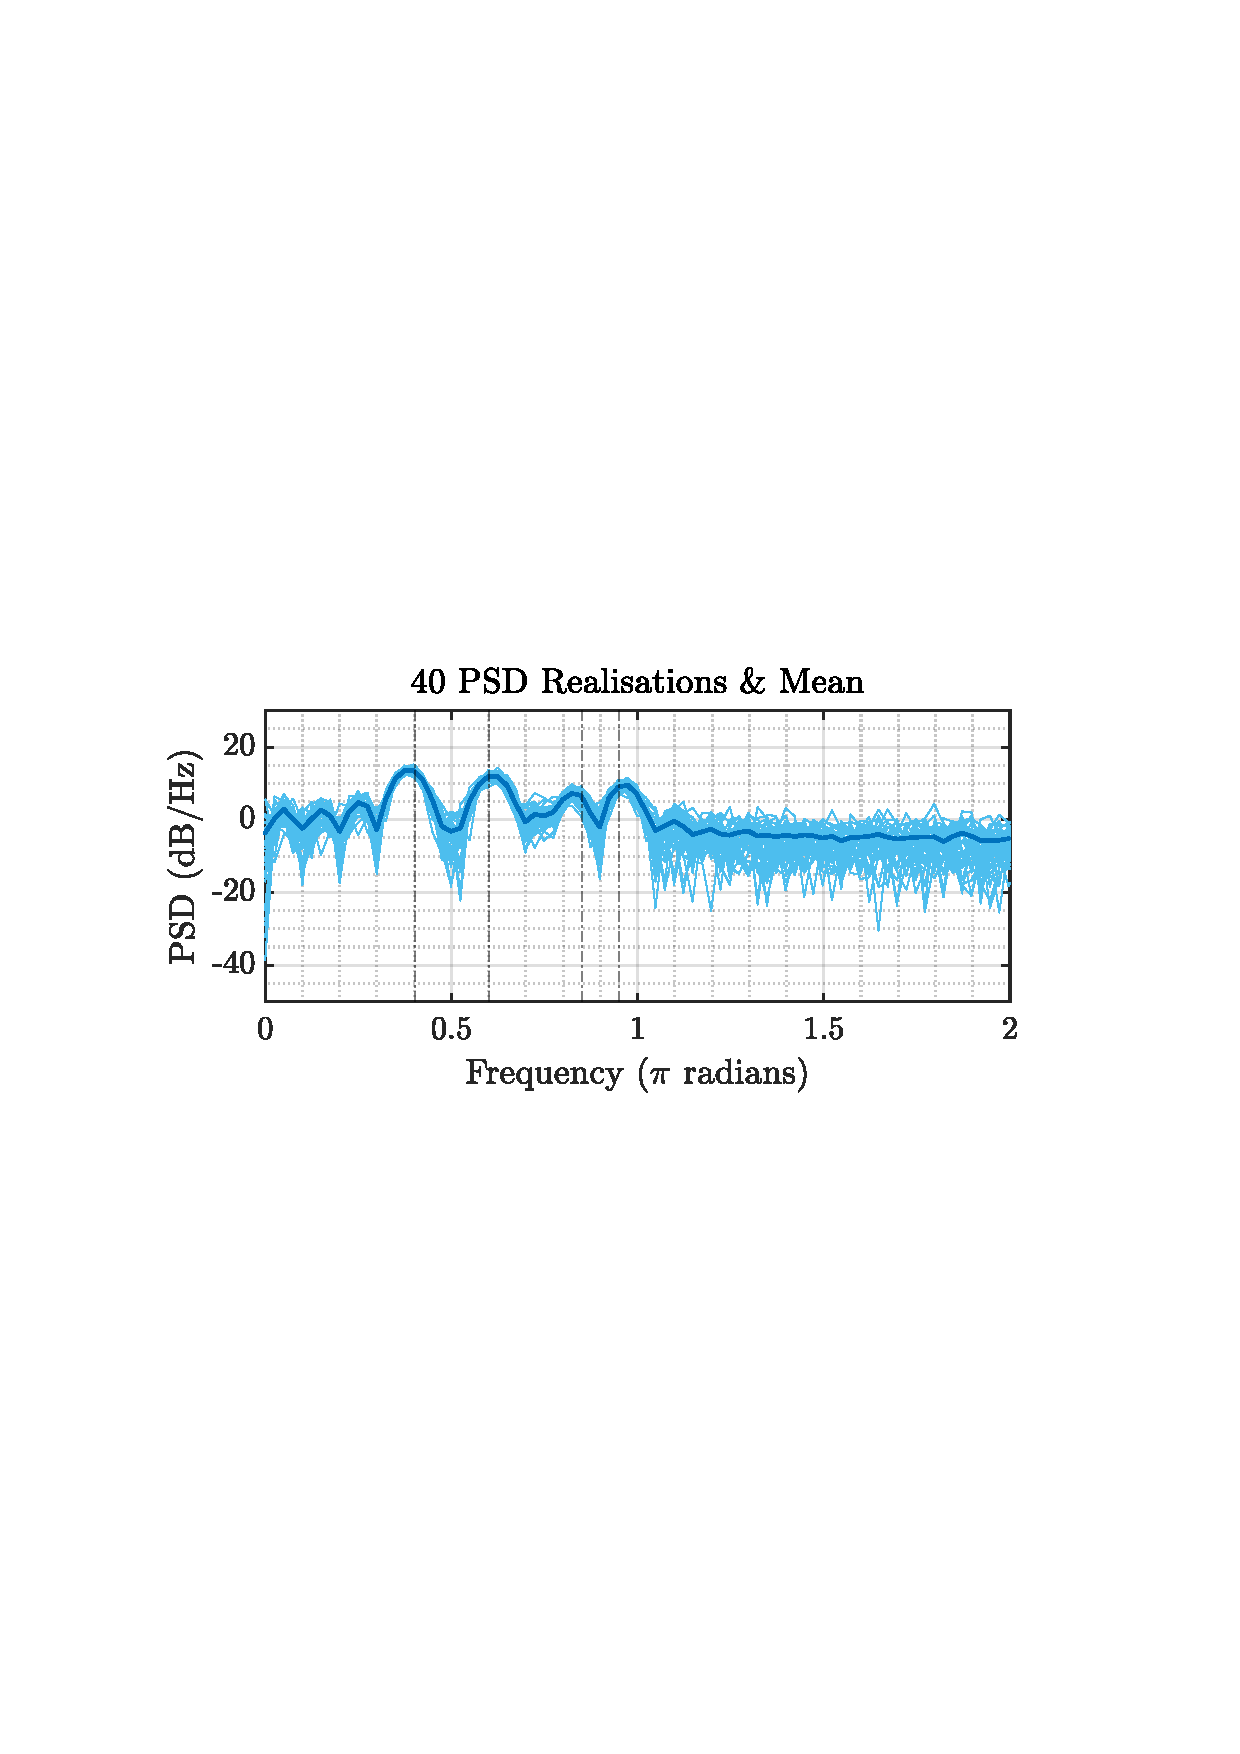
\includegraphics[trim={2.2cm 11.2cm 3.15cm  11.2cm}, clip, width=\textwidth]{../MATLAB/figures/q1_3c_fig01.pdf} 
			\captionsetup{justification=centering}
			\caption{Periodogram}
		\end{subfigure}
		%		~ % forces onto the same row
		\begin{subfigure}{0.49\textwidth}
			\centering
			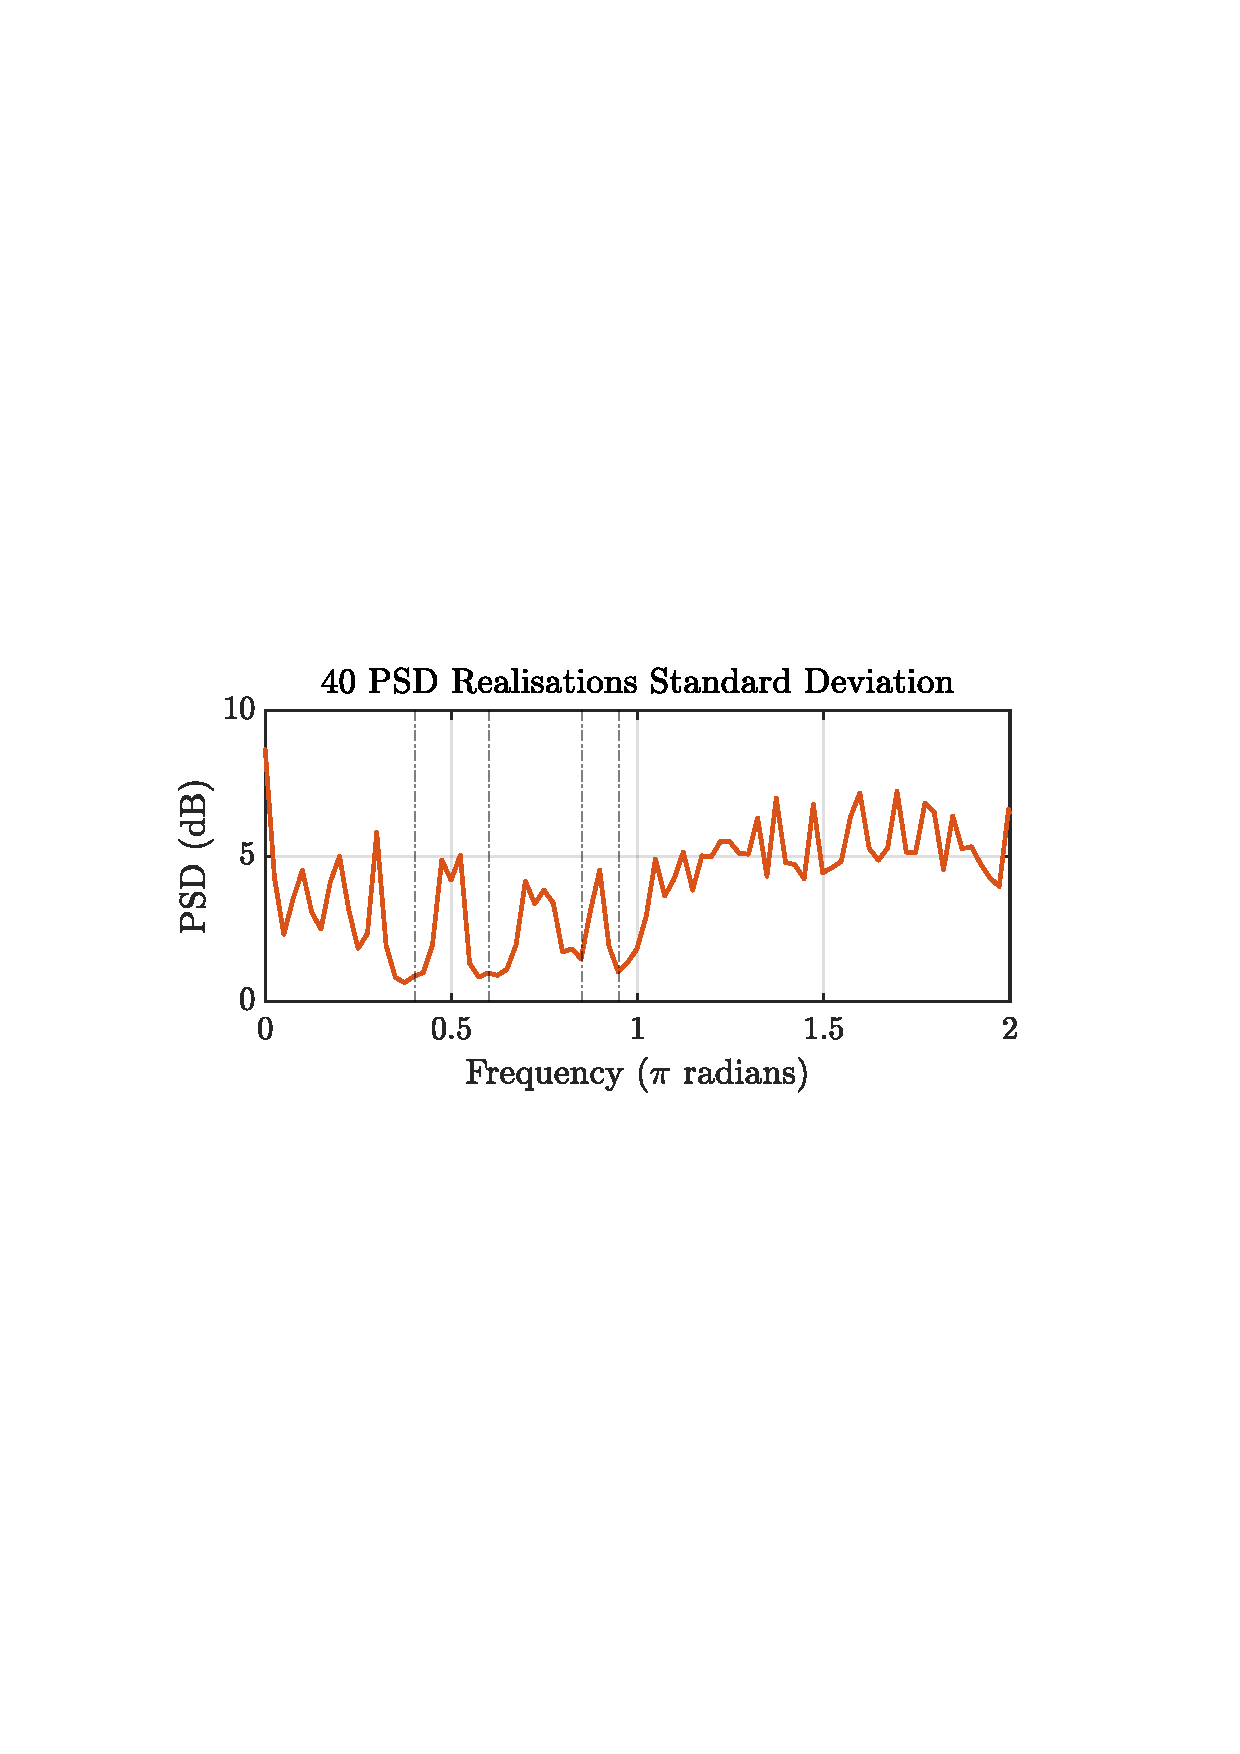
\includegraphics[trim={2.2cm 11.2cm 3.15cm  11.2cm}, clip, width=\textwidth]{../MATLAB/figures/q1_3c_fig02.pdf} 
			\captionsetup{justification=centering}
			\caption{Standard Deviation}
		\end{subfigure}
		\captionsetup{justification=centering}
		\caption{The total number of data points used was 512, black vertical lines indicate the model defined frequencies}
		\label{fig: 1-3c}
	\end{figure}

	Figure \ref{fig: 1-3c}. It is advantageous that the standard deviation decreases around our frequencies of interest instead of increases. 

	\subsubsection{Influence of Data Samples on the PSD}
	
	\begin{figure}[H]%{R}{0.49\textwidth}
%	\begin{figure}[H]
		\centering
			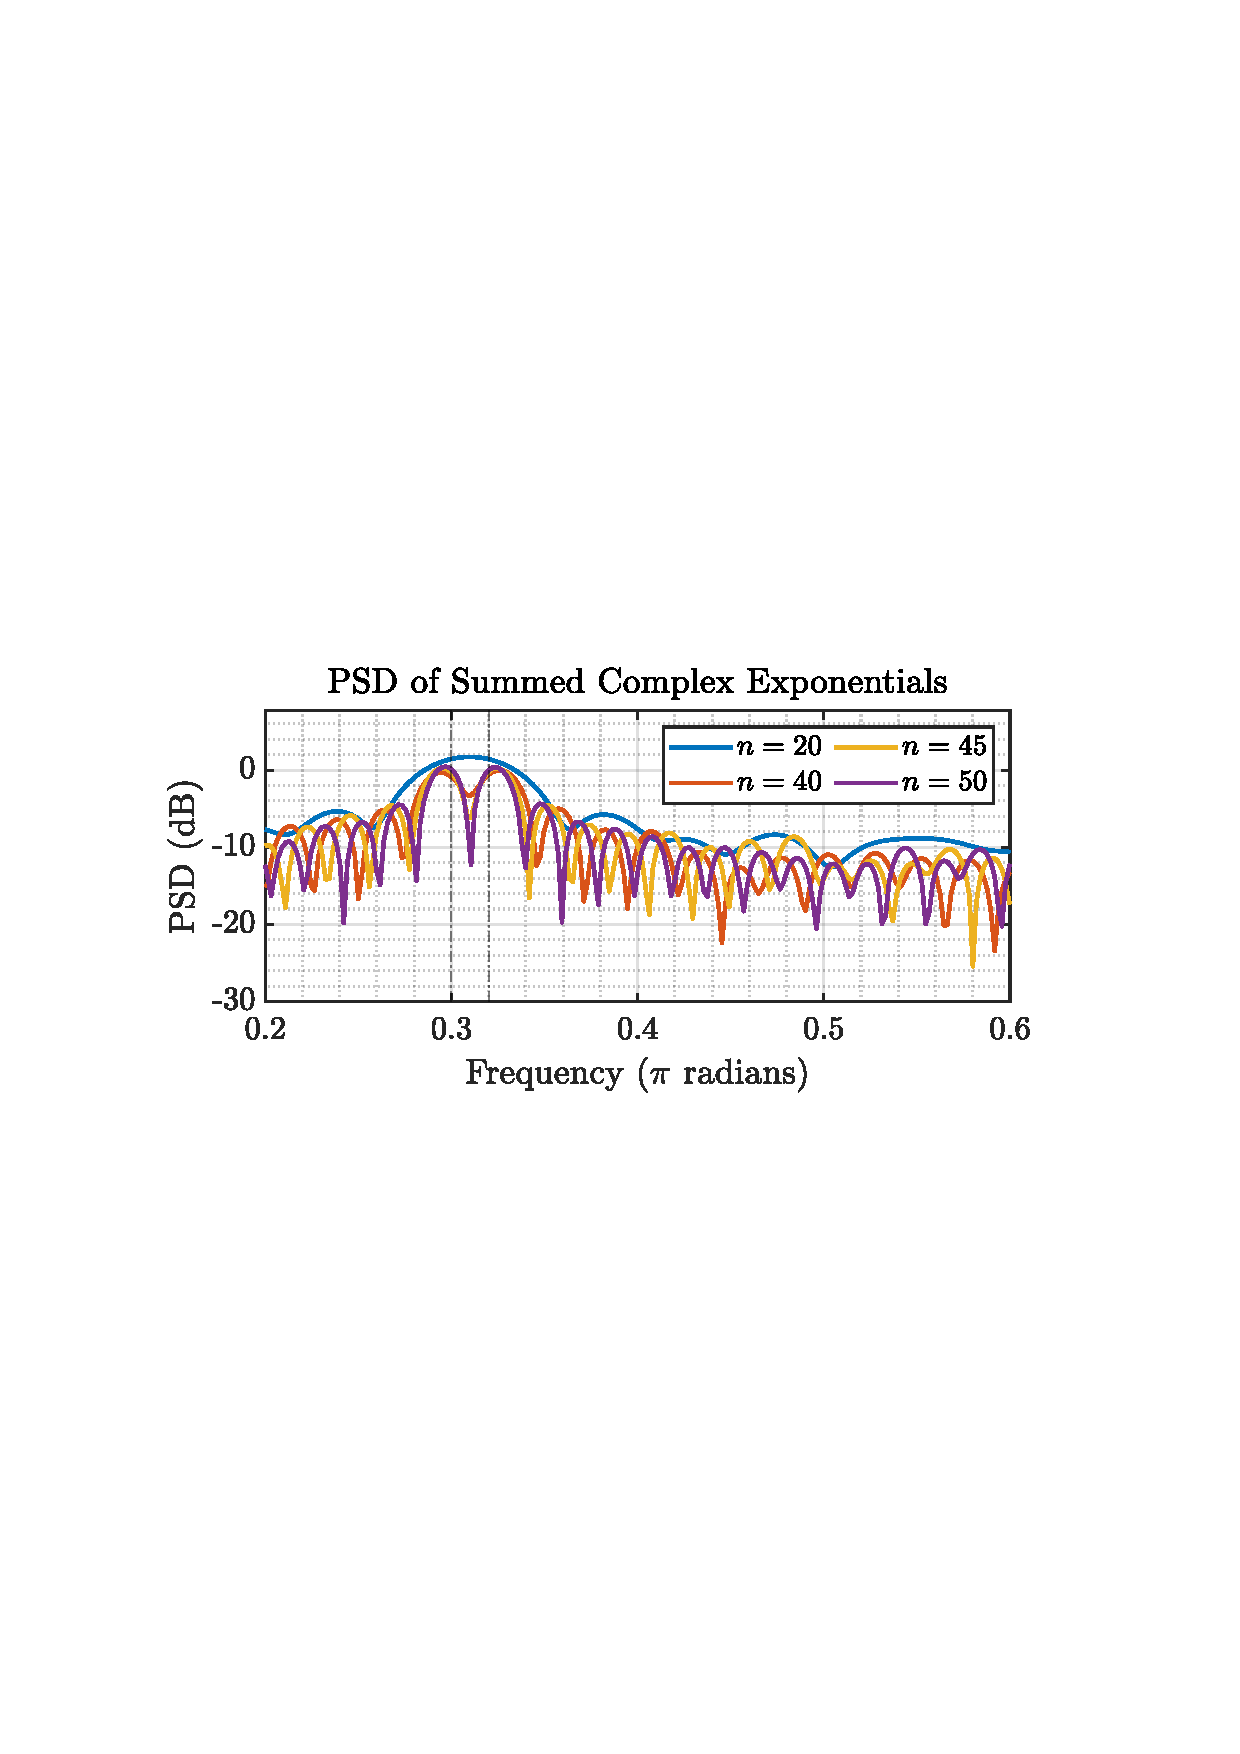
\includegraphics[trim={2.2cm 11.2cm 3.15cm  11.2cm}, clip, width=0.49\textwidth]{../MATLAB/figures/q1_3d_fig01.pdf} 
%		\end{centering}
%	\end{figure}
	\captionsetup{justification=centering}
	\caption{PSD while varying $n$, the number of Data Samples used}
	\label{fig: 1-3d}
	\end{figure}
	
	In Figure \ref{fig: 1-3d} we can clearly see that the frequency resolution is insufficient at lower sample numbers, resulting in aliasing of the desired frequency peaks.
	
	\subsubsection{MUltiple SIgnal Classification (MUSIC) Estimator}
	
	\begin{figure}[H]
		\centering
		\begin{subfigure}{0.49\textwidth}
			\centering
			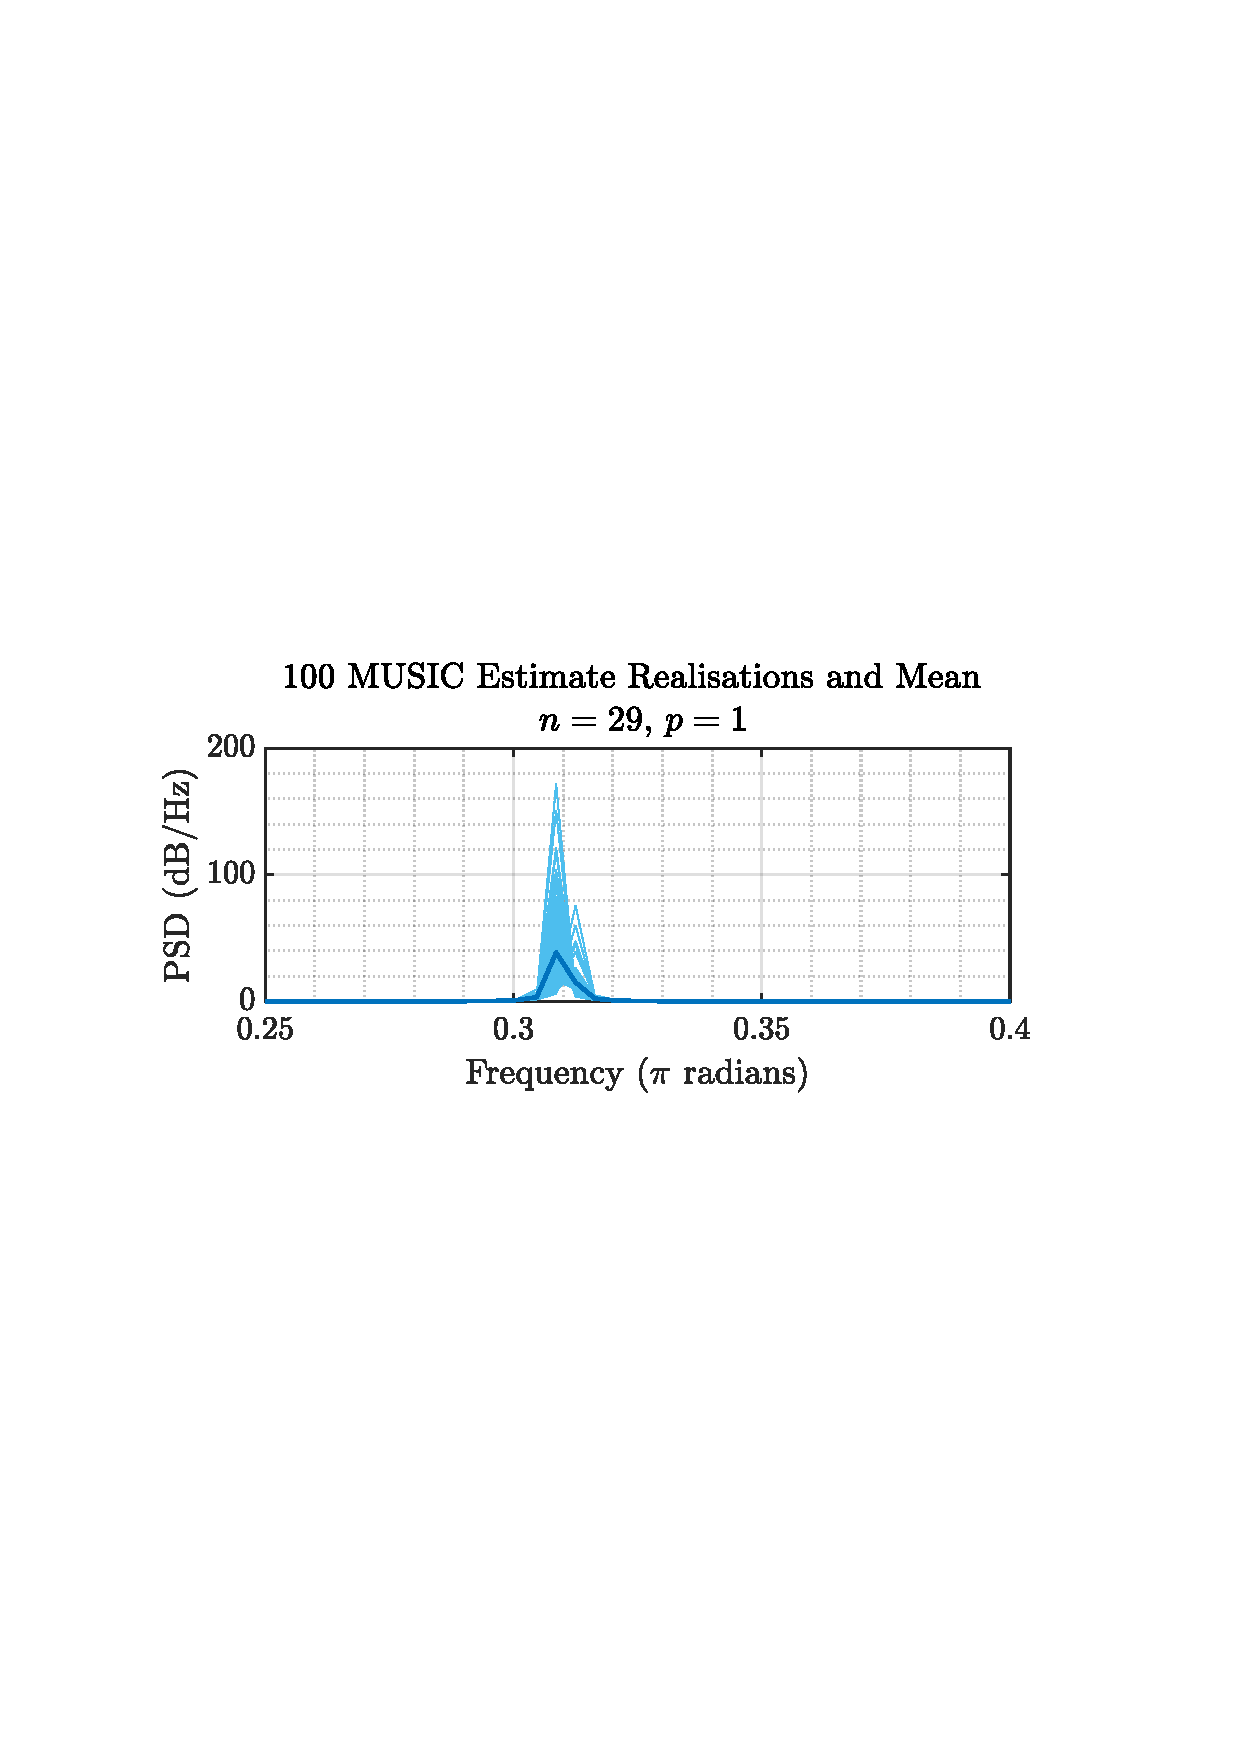
\includegraphics[trim={2.2cm 11cm 3.15cm  11.2cm}, clip, width=\textwidth]{../MATLAB/figures/q1_3e_fig01.pdf} 
		\end{subfigure}
		%		~ % forces onto the same row
		\begin{subfigure}{0.49\textwidth}
			\centering
			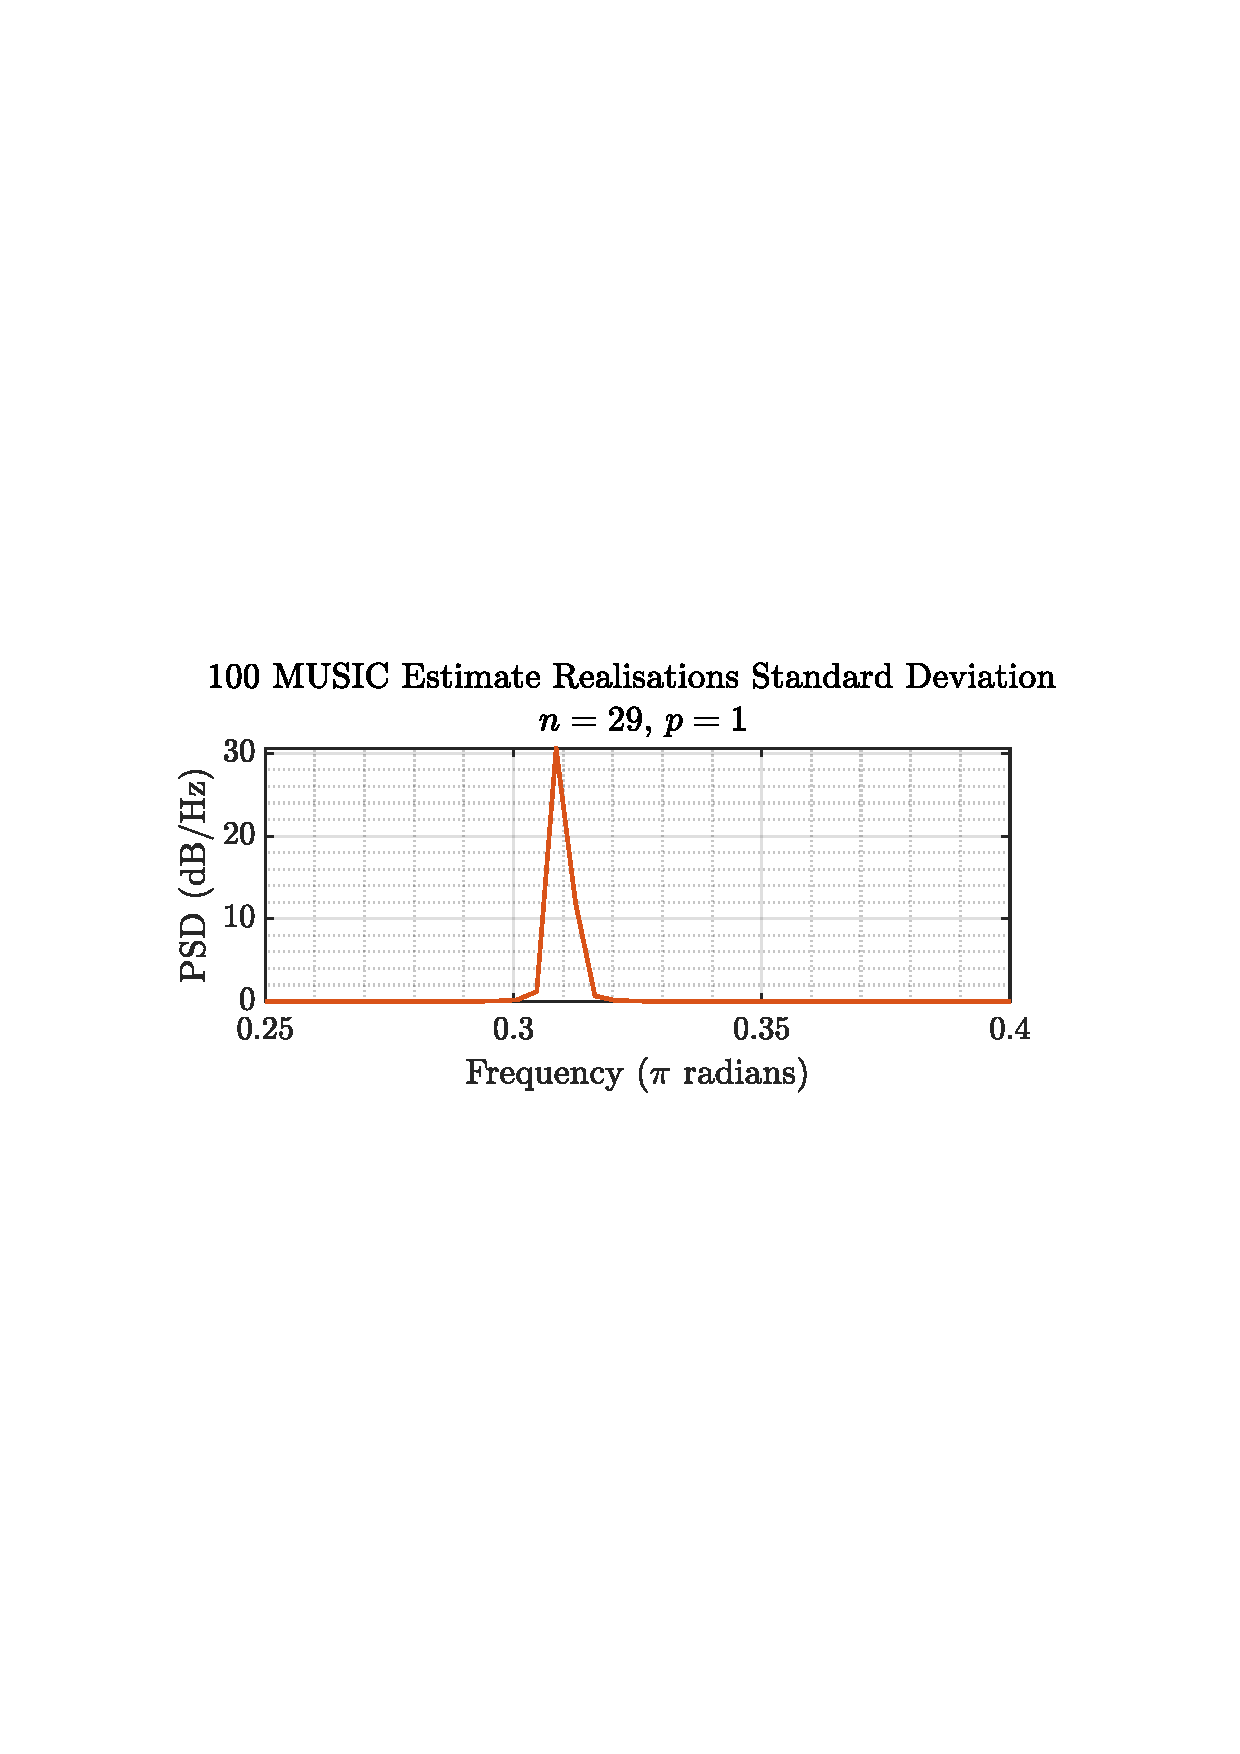
\includegraphics[trim={2.2cm 11cm 3.15cm  11.2cm}, clip, width=\textwidth]{../MATLAB/figures/q1_3e_fig02.pdf} 
		\end{subfigure}
		\begin{subfigure}{0.49\textwidth}
			\centering
			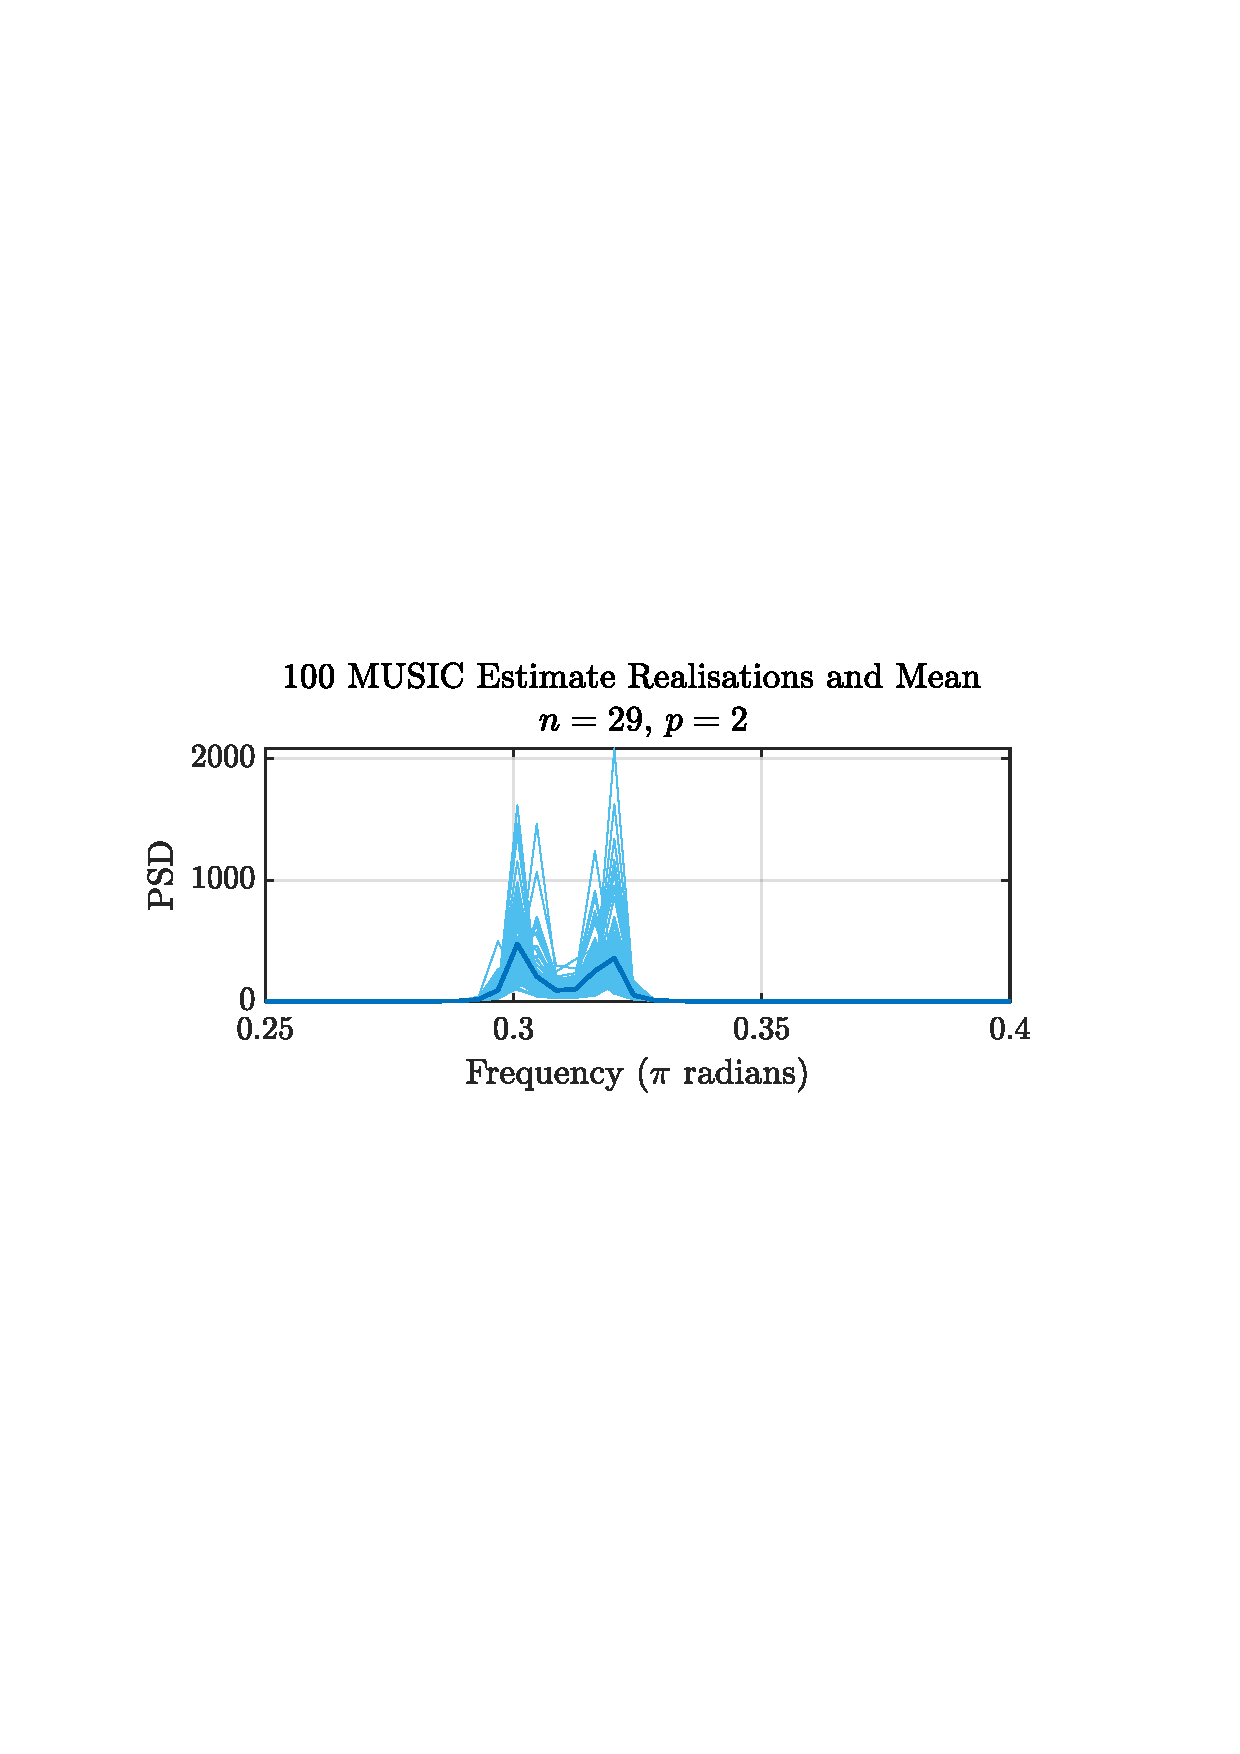
\includegraphics[trim={2.2cm 11cm 3.15cm  11.2cm}, clip, width=\textwidth]{../MATLAB/figures/q1_3e_fig03.pdf} 
		\end{subfigure}
		%		~ % forces onto the same row
		\begin{subfigure}{0.49\textwidth}
			\centering
			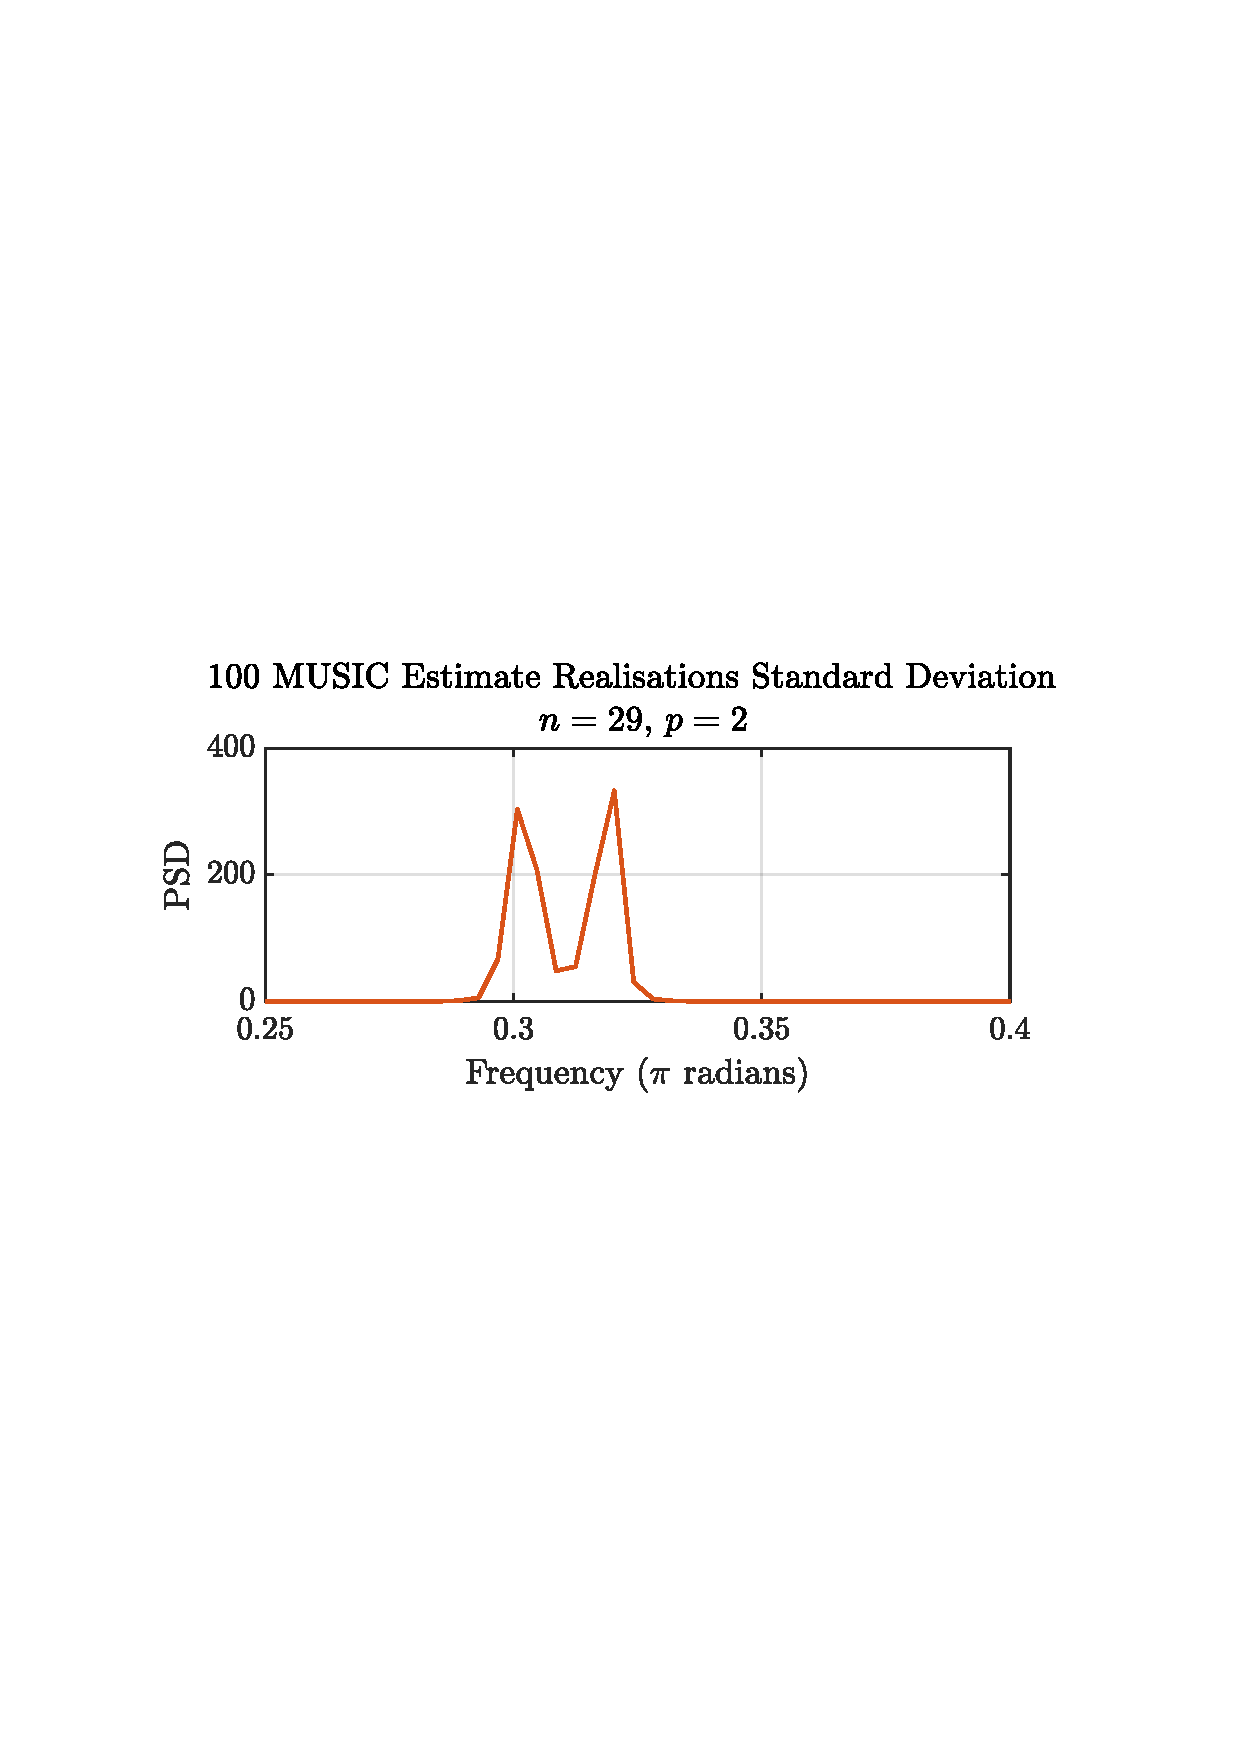
\includegraphics[trim={2.2cm 11cm 3.15cm  11.2cm}, clip, width=\textwidth]{../MATLAB/figures/q1_3e_fig04.pdf} 
		\end{subfigure}
		\begin{subfigure}{0.49\textwidth}
			\centering
			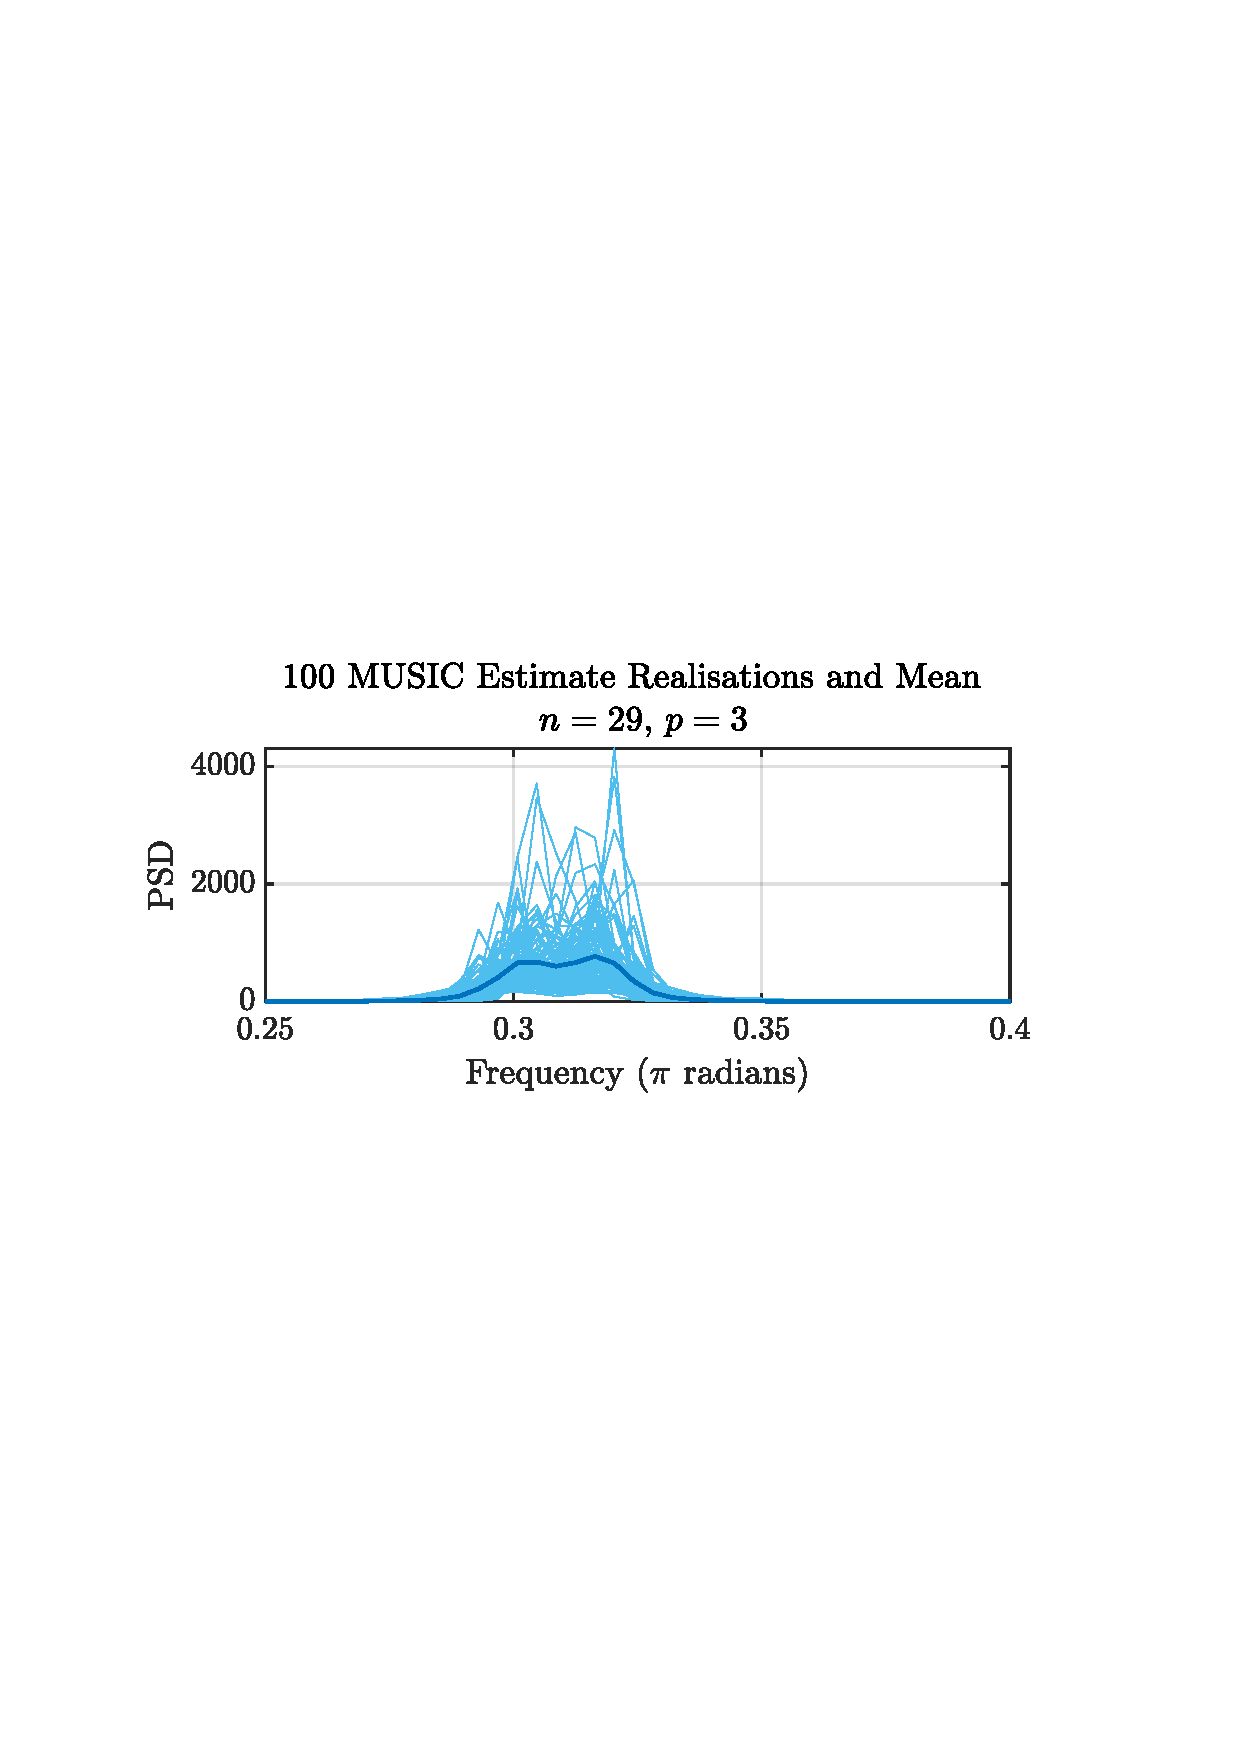
\includegraphics[trim={2.2cm 11.2cm 3.15cm  11.2cm}, clip, width=\textwidth]{../MATLAB/figures/q1_3e_fig05.pdf} 
		\end{subfigure}
		%		~ % forces onto the same row
		\begin{subfigure}{0.49\textwidth}
			\centering
			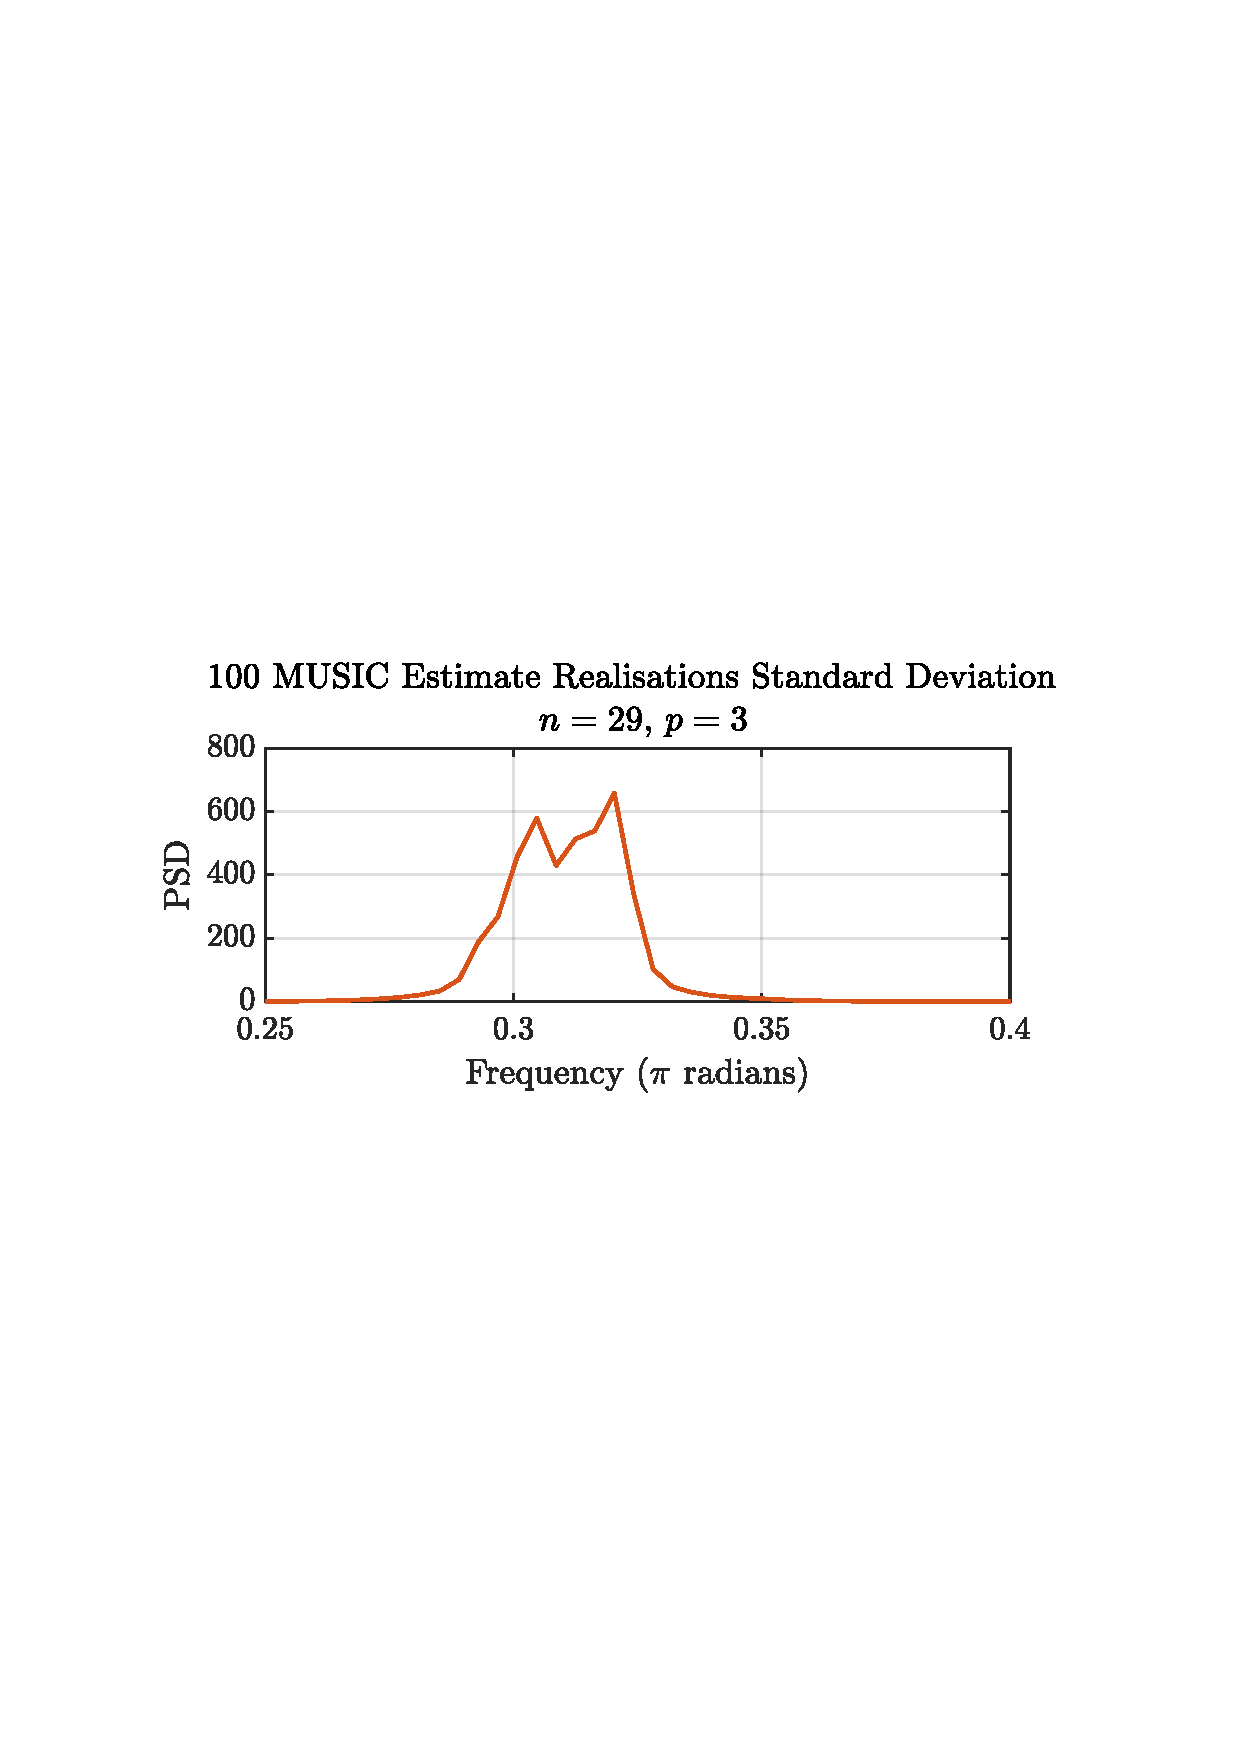
\includegraphics[trim={2.2cm 11.2cm 3.15cm  11.2cm}, clip, width=\textwidth]{../MATLAB/figures/q1_3e_fig06.pdf} 
		\end{subfigure}
		\captionsetup{justification=centering}
		\caption{Set of Auto-Correlation Functions (ACFs) and their Correlograms. \\ $n$ is the number of samples used, $p$ is the Signal Space Dimensionality}
		\label{fig: 1-3e}
	\end{figure}

	The MUSIC estimate identifies eigenvalues of an autocorrelation matrix in descending magnitude order - which indicate directions of largest variability in the subspace. \\
	The first line creates the 14 dimensional modified correlation matrix $R_{xx}$ for the dataset, which is subsequently used by the MUSIC algorithm with $p$ setting the Signal Subspace Dimensionality in the second line. \\
	The third line plots the Pseudospectrum (PSD Estimate) against the frequency axis. \\
	
	Figure \ref{fig: 1-3e} shows the MUSIC estimate plots for the given equation. The spectrum is not very detailed, peaks are not all sharp, but are clearly distinguishable from the surrounding periodogram. In the general case the MUSIC estimator is a good choice if the signal space dimensionality is known, especially as it works on such a limited set of samples. \\
	
	The periodogram is equally suitable for resolving peaks, but requires more samples for a meaningful resolution. \\
	
	In both periodogram and MUSIC estimators we see that the standard deviation, hence variance increase around the peaks, except when using the log scale of the periodogram, where it decreases.
	
	% TODO: A figure doing a direct comparison for the same signal maybe.
	
	% TODO: Bias and Variance
	
	\subsection{Spectrum of Autoregressive (AR) Processes} \label{sec: 1-4-spectrums-AR}

	
	\subsubsection{Shortcomings of the Unbiased ACF in finding AR Parameters}
	
	As the unbiased estimator allows for negative values, at a computational level it will require more bits to store, especially for larger values.
	
	\subsubsection{Error of the AR PSD Estimate}
	\begin{figure}[H]
		\centering
		\begin{subfigure}{0.49\textwidth}
			\centering
			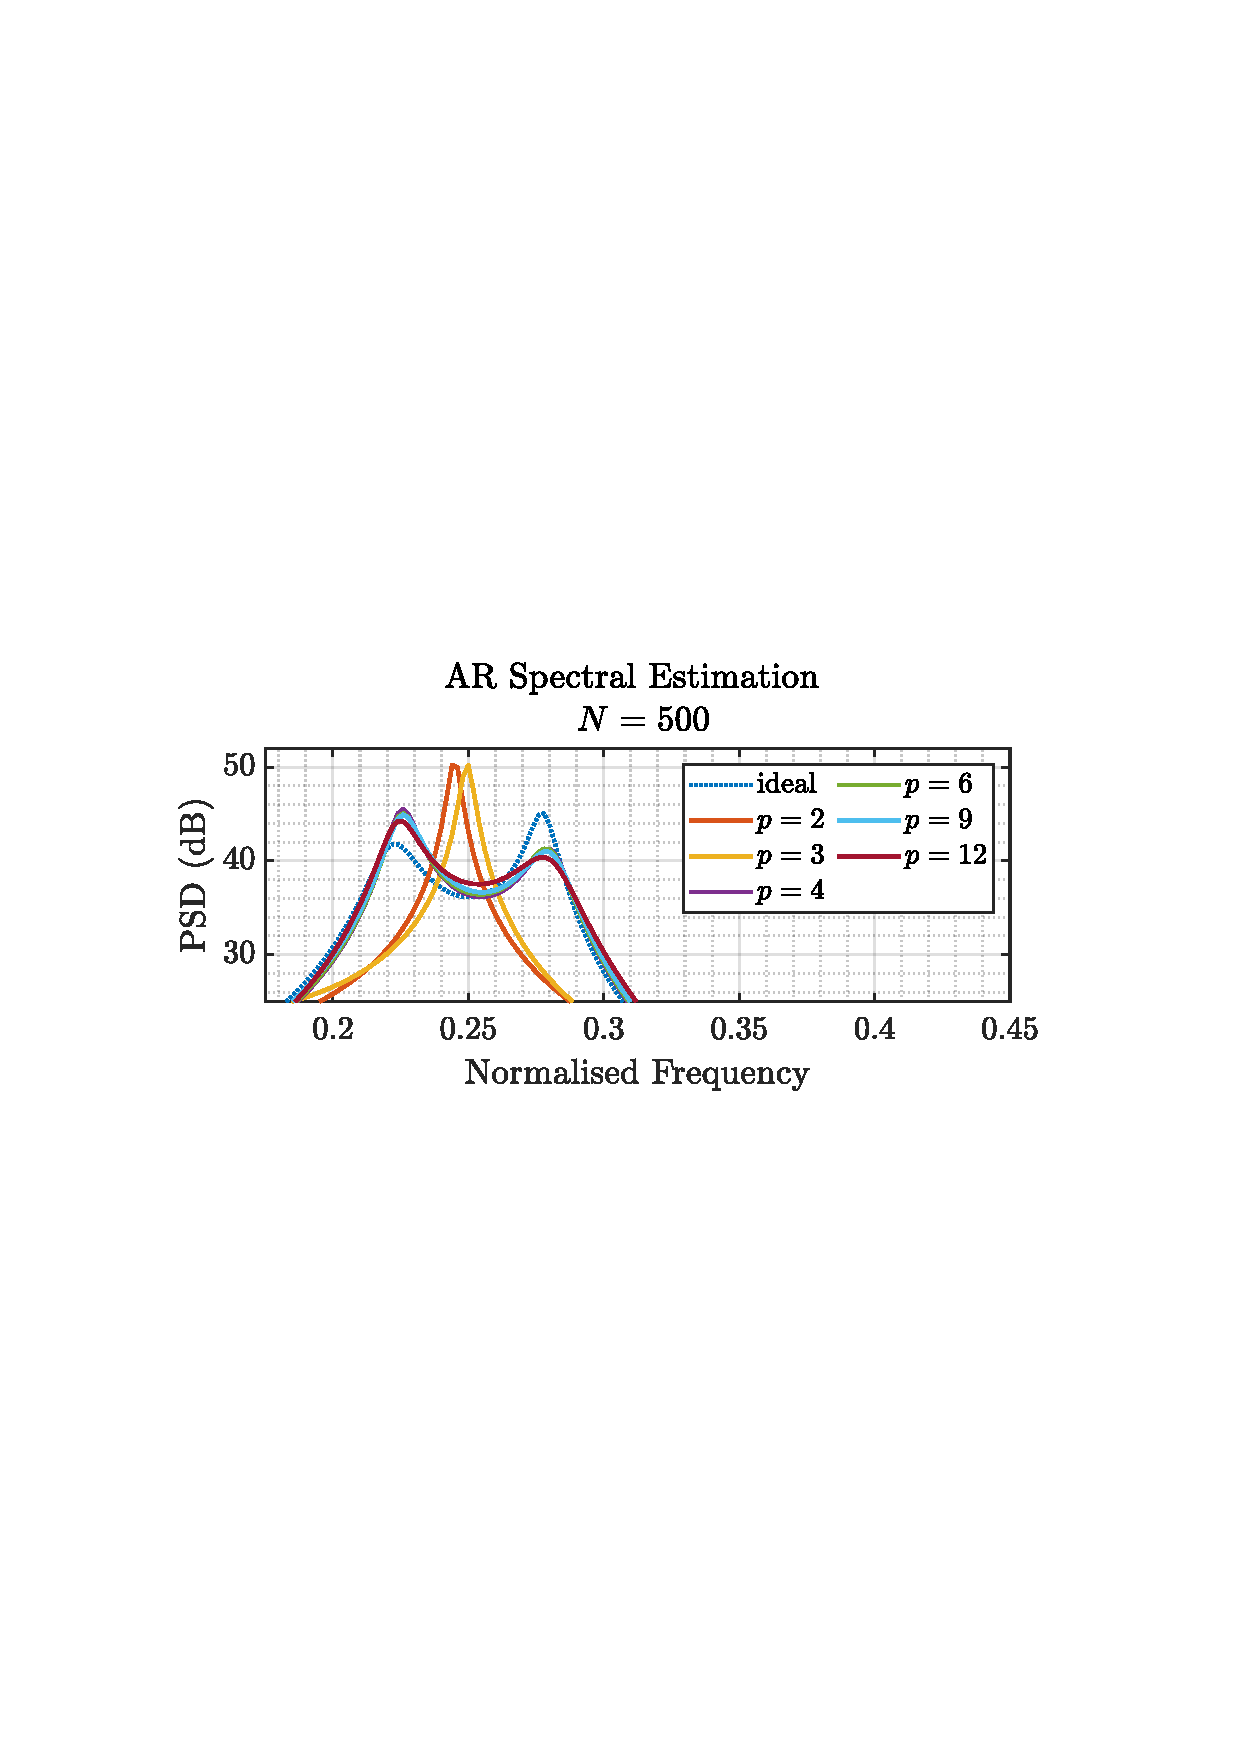
\includegraphics[trim={2.2cm 11.2cm 3.15cm  11.2cm}, clip, width=\textwidth]{../MATLAB/figures/q1_4b_fig14.pdf} 
			\captionsetup{justification=centering}
			\caption{AR Periodogram and its $p$ Order Estimates}
		\end{subfigure}
		%		~ % forces onto the same row
		\begin{subfigure}{0.49\textwidth}
			\centering
			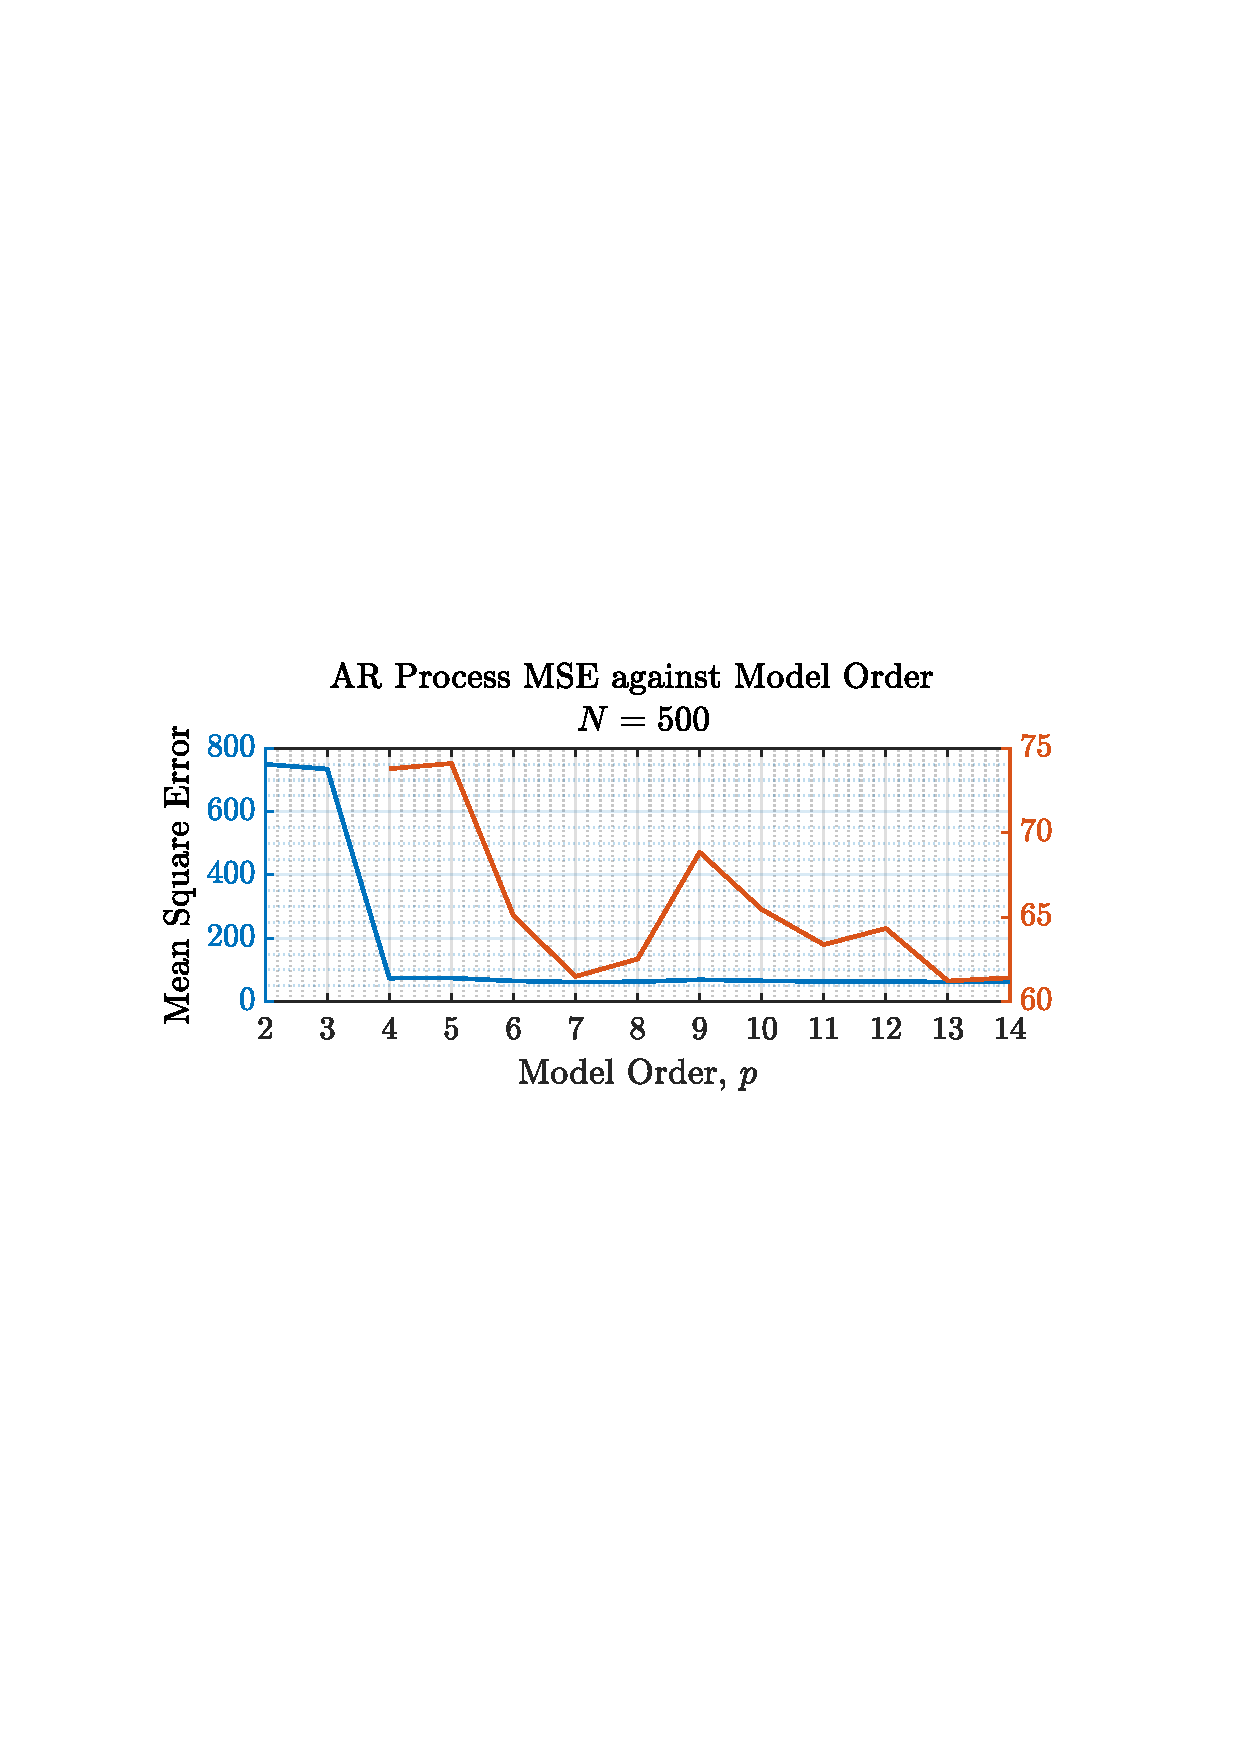
\includegraphics[trim={2.2cm 11.2cm 3.15cm  11.2cm}, clip, width=\textwidth]{../MATLAB/figures/q1_4b_fig16.pdf} 
			\captionsetup{justification=centering}
			\caption{Mean Squared Error with two y-scales}
		\end{subfigure}
		\captionsetup{justification=centering}
		\caption{}
		\label{fig: 1-4b}
	\end{figure}

	We can see in (a) of \ref{fig: 1-4b}, that increasing the order tends towards a better solution. But (b) notes that the most drastic difference is at the model order, 4, which matches the order of the process defined, subsequent increases of the model order do increase its likeliness to the true response, but changes are not so drastic.
	

	\subsubsection{Error of the AR PSD Estimate with more Samples}
	\begin{figure}[H]
		\centering
		\begin{subfigure}{0.49\textwidth}
			\centering
			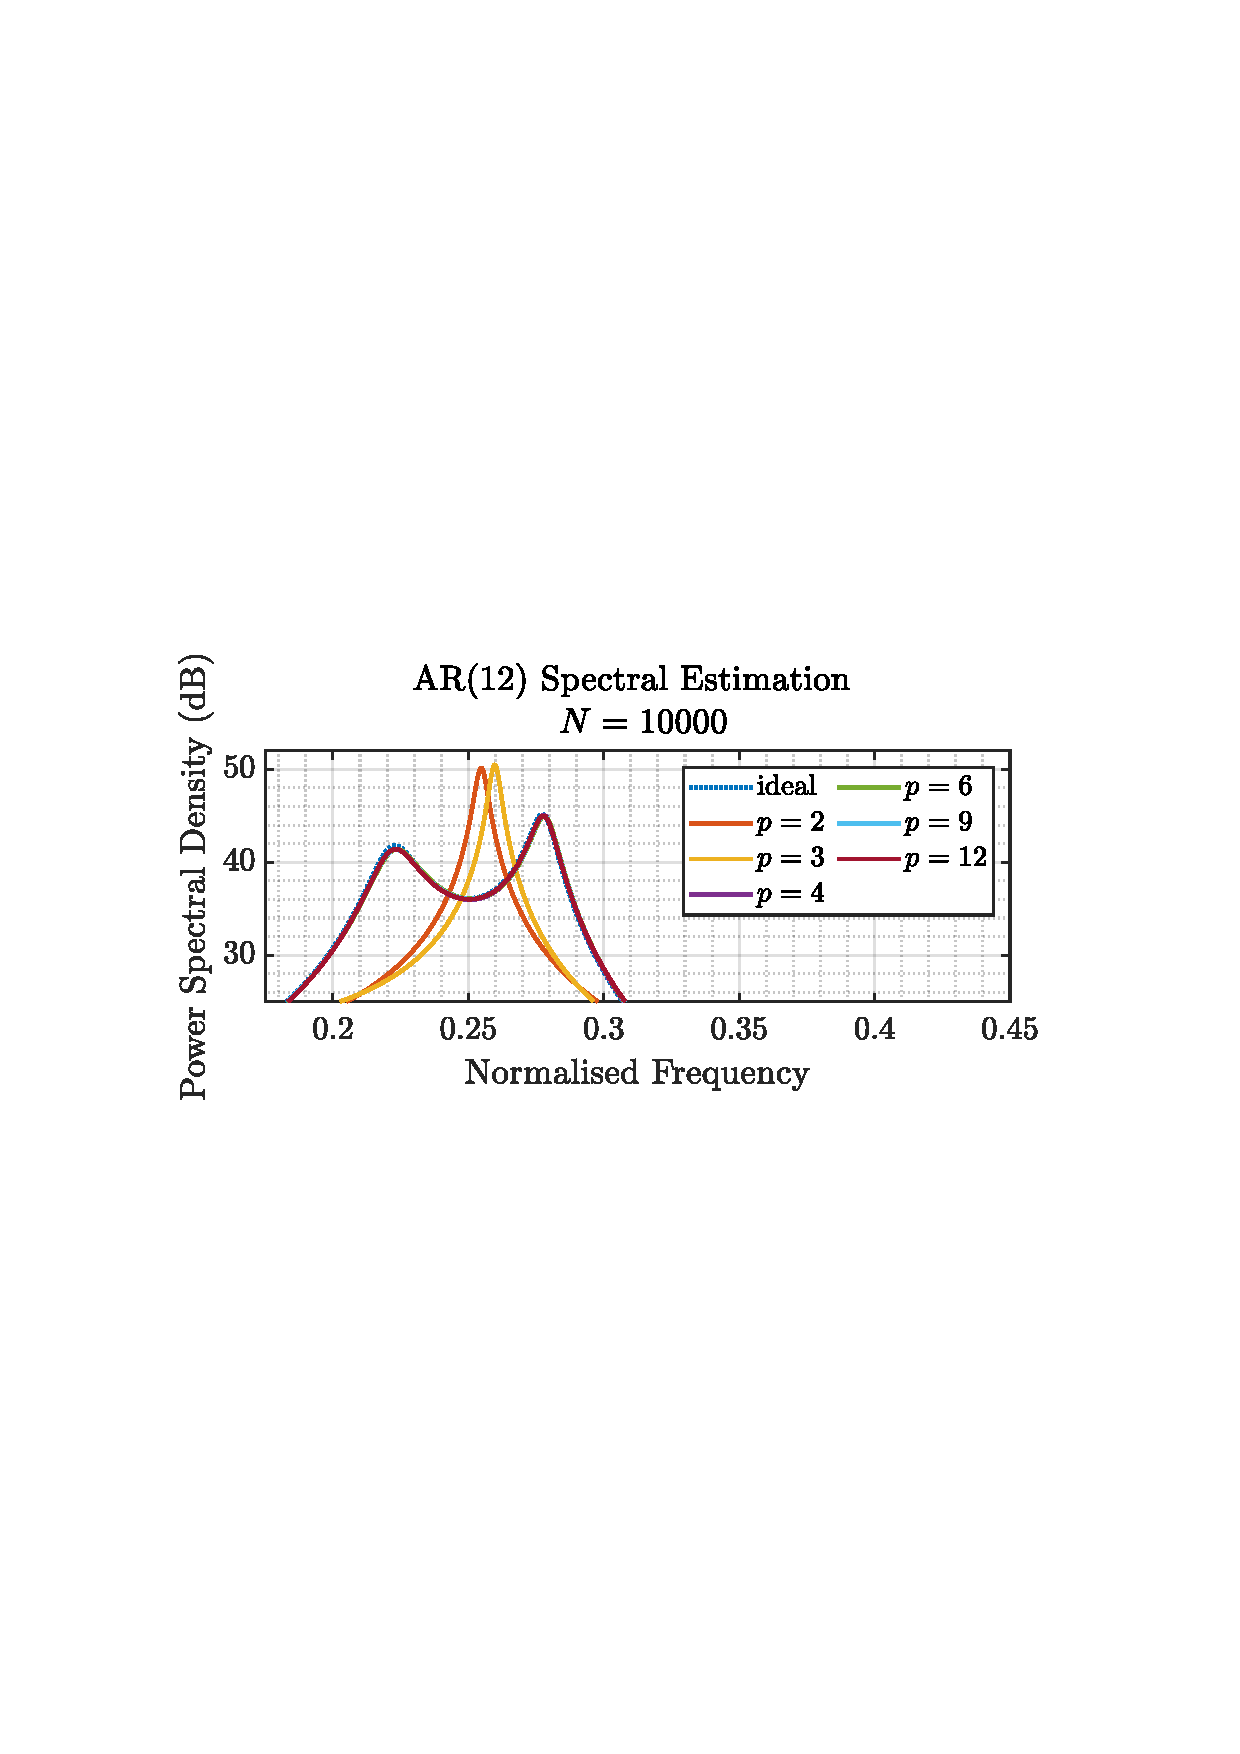
\includegraphics[trim={2.2cm 11.2cm 3.15cm  11.2cm}, clip, width=\textwidth]{../MATLAB/figures/q1_4c_fig14.pdf} 
			\captionsetup{justification=centering}
			\caption{AR Periodogram and its $p$ Order Estimates}
		\end{subfigure}
		%		~ % forces onto the same row
		\begin{subfigure}{0.49\textwidth}
			\centering
			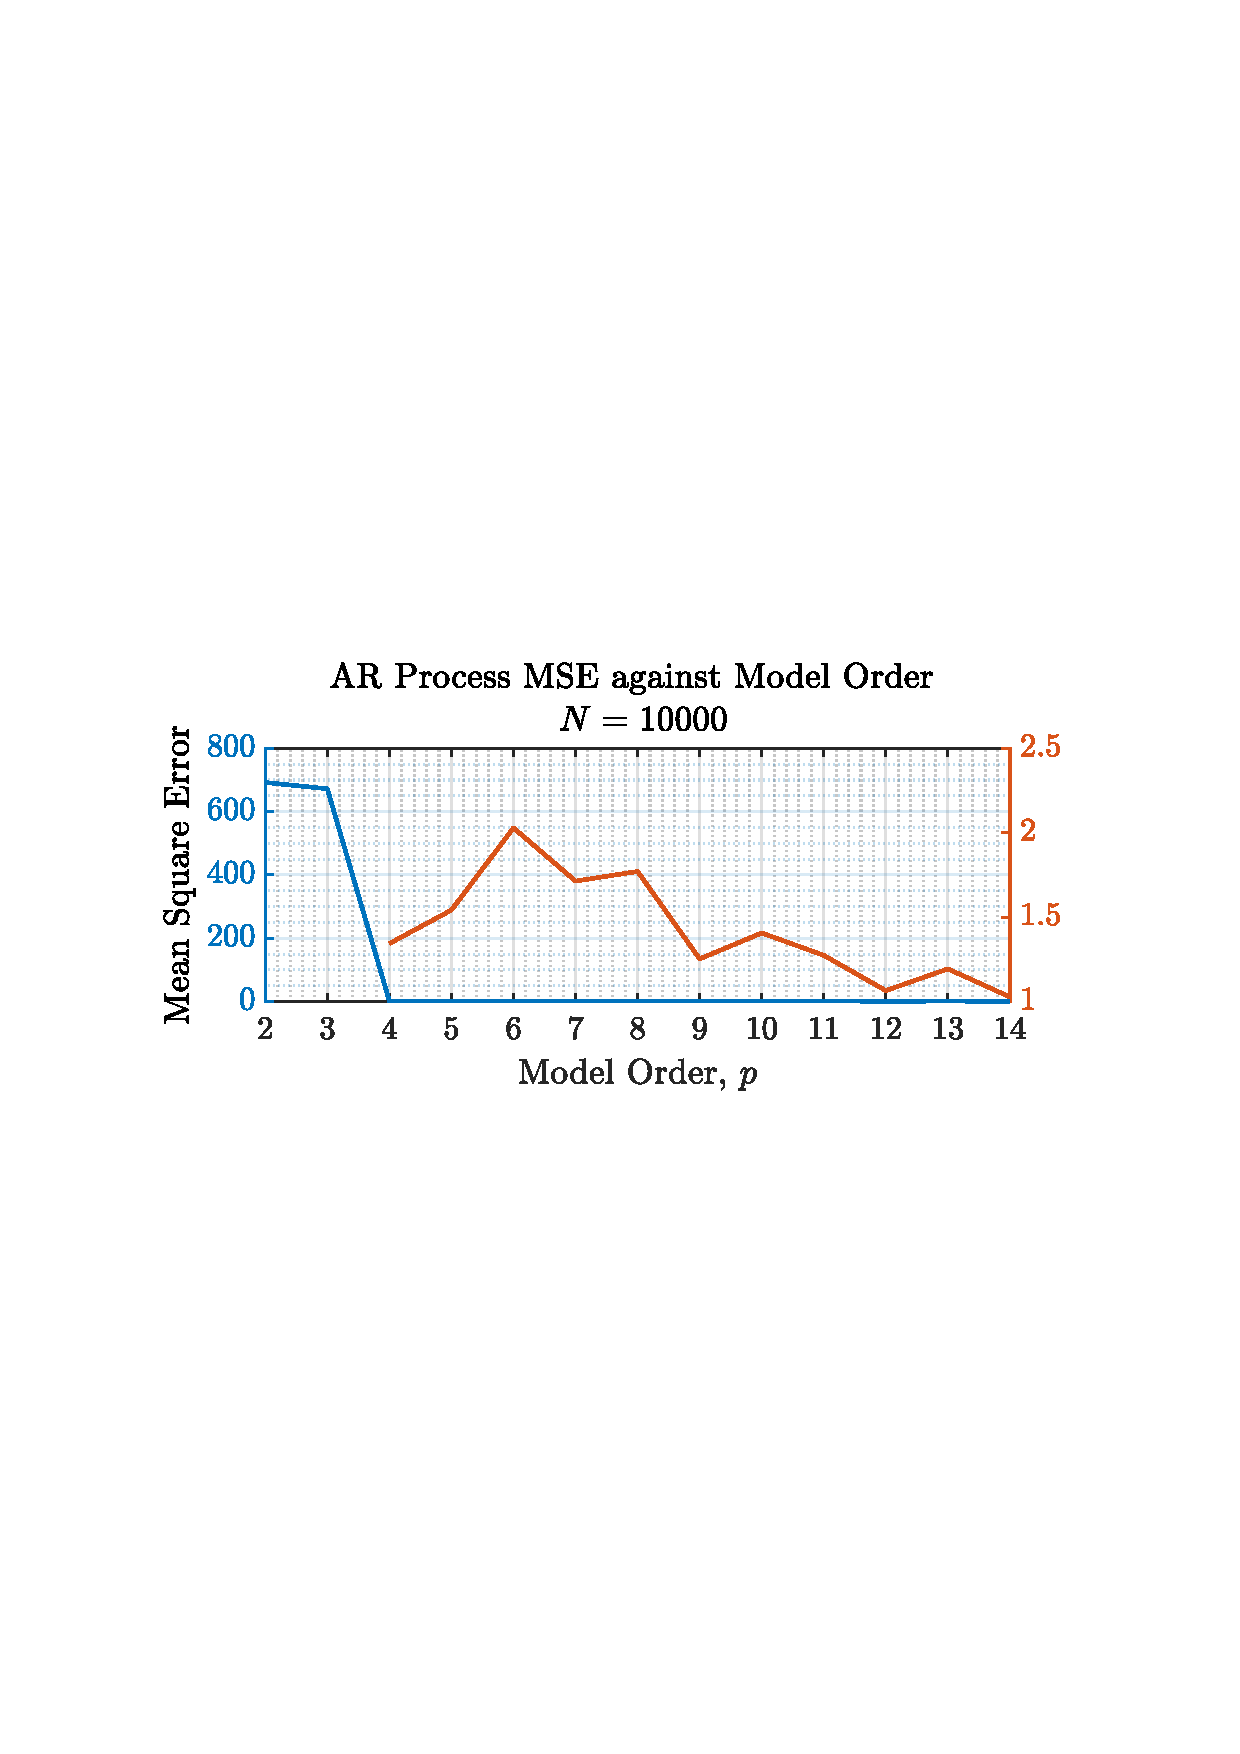
\includegraphics[trim={2.2cm 11.2cm 3cm  11.2cm}, clip, width=\textwidth]{../MATLAB/figures/q1_4c_fig16.pdf} 
			\captionsetup{justification=centering}
			\caption{Mean Squared Error with two y-scales}
		\end{subfigure}
		\captionsetup{justification=centering}
		\caption{}
		\label{fig: 1-4c}
	\end{figure}

	The same trend is seen in Figure \ref{fig: 1-4c}, as we saw with $N=500$, although the estimate now matches the underlying model much better, reflected in the drastically lower MSE. \\
	
	It is noted that for a more valid comparison of model order's influence on the estimate's error the Akaike Information Criterion (AIC) or the Bayesian Information Criterion (BIC) are more suitable quantifiers of model order suitability than MSE. But the accuracy trend reflected in the MSE is still valid for our comparisons.
	
	\pagebreak
	
	\subsection{Real World Signals: Respiratory Sinus Arrhythmia from RR-Intervals} \label{sec: 1-5-real-world-signals}
	
	\subsubsection{Standard \& Average PSDs of the RRI Dataset}
	\begin{figure}[H]
		\centering
		\begin{subfigure}{0.49\textwidth}
			\centering
			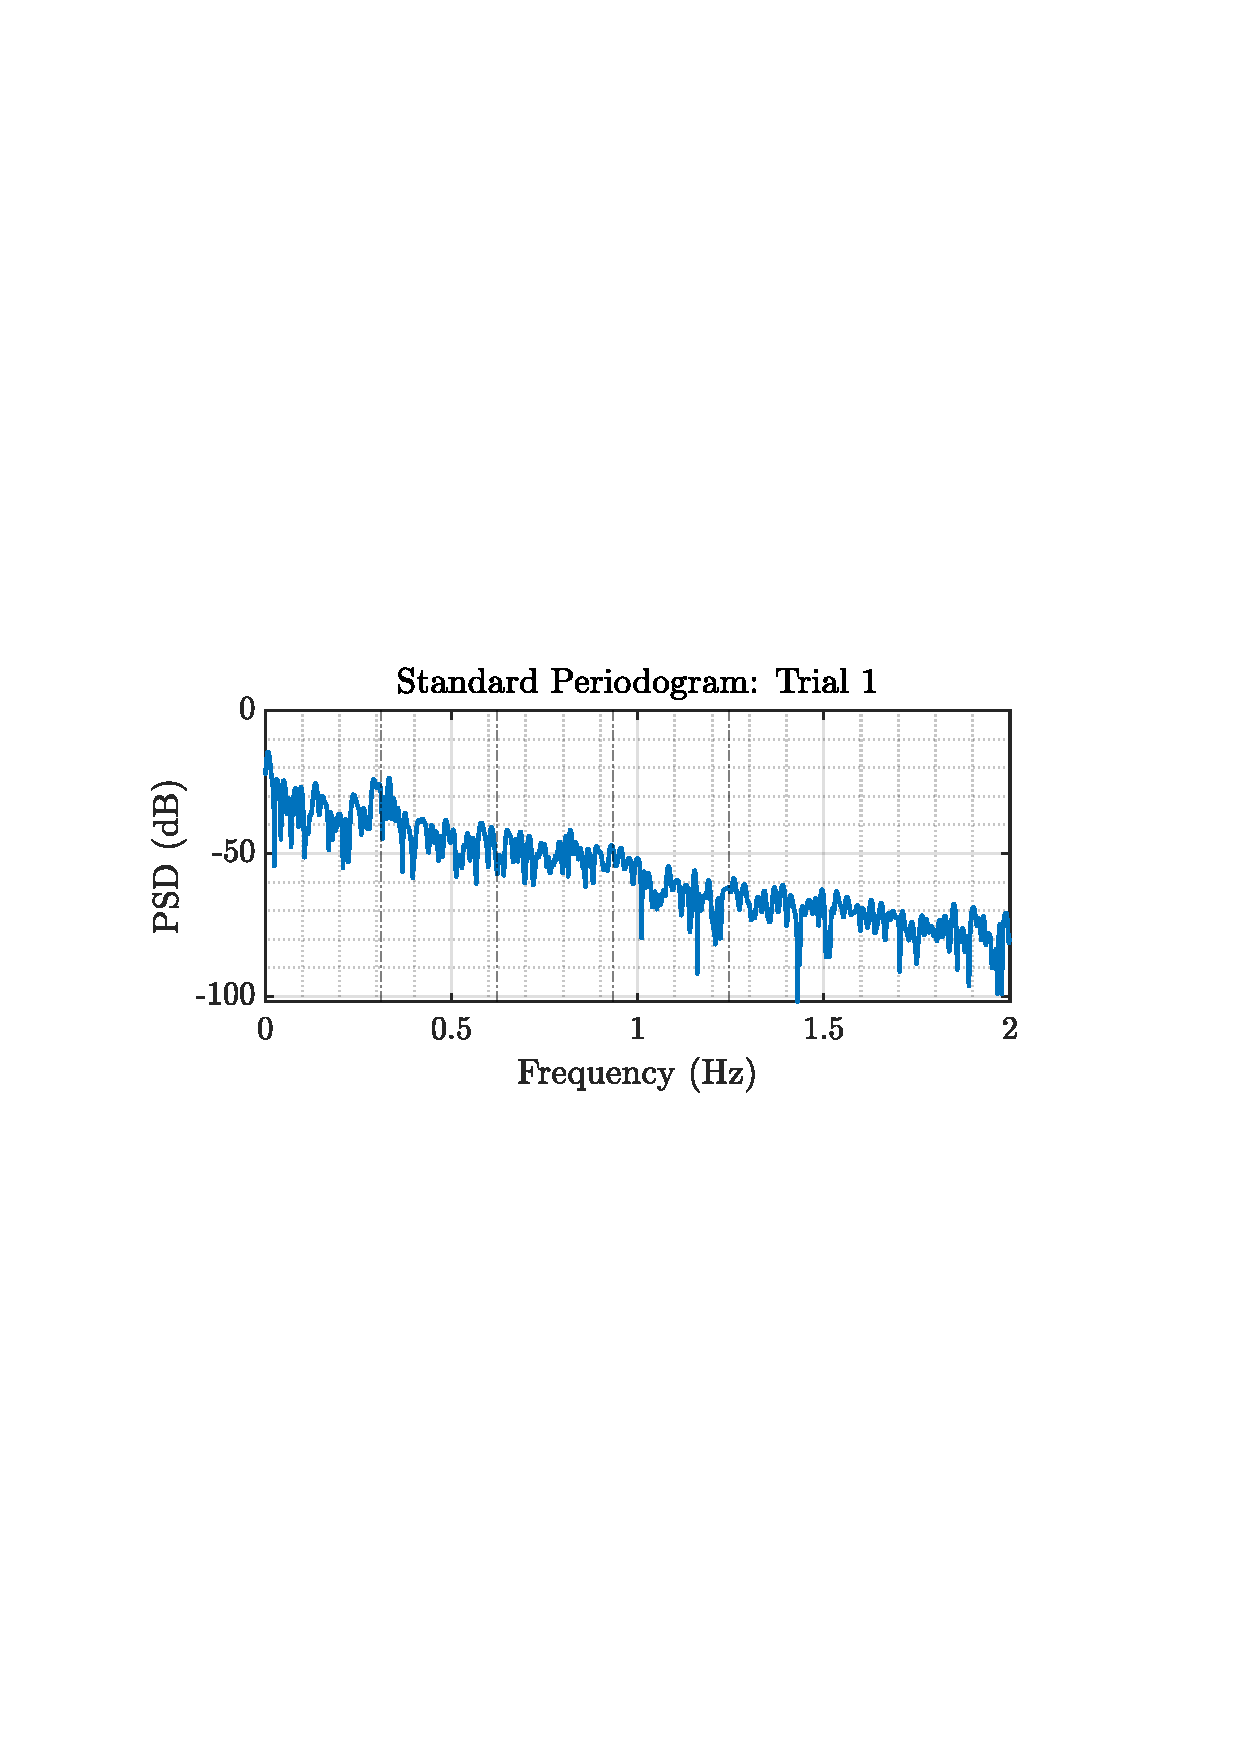
\includegraphics[trim={2.2cm 11cm 3.15cm  11.2cm}, clip, width=\textwidth]{../MATLAB/figures/q1_5a_fig01.pdf} 
		\end{subfigure}
		%		~ % forces onto the same row
		\begin{subfigure}{0.49\textwidth}
			\centering
			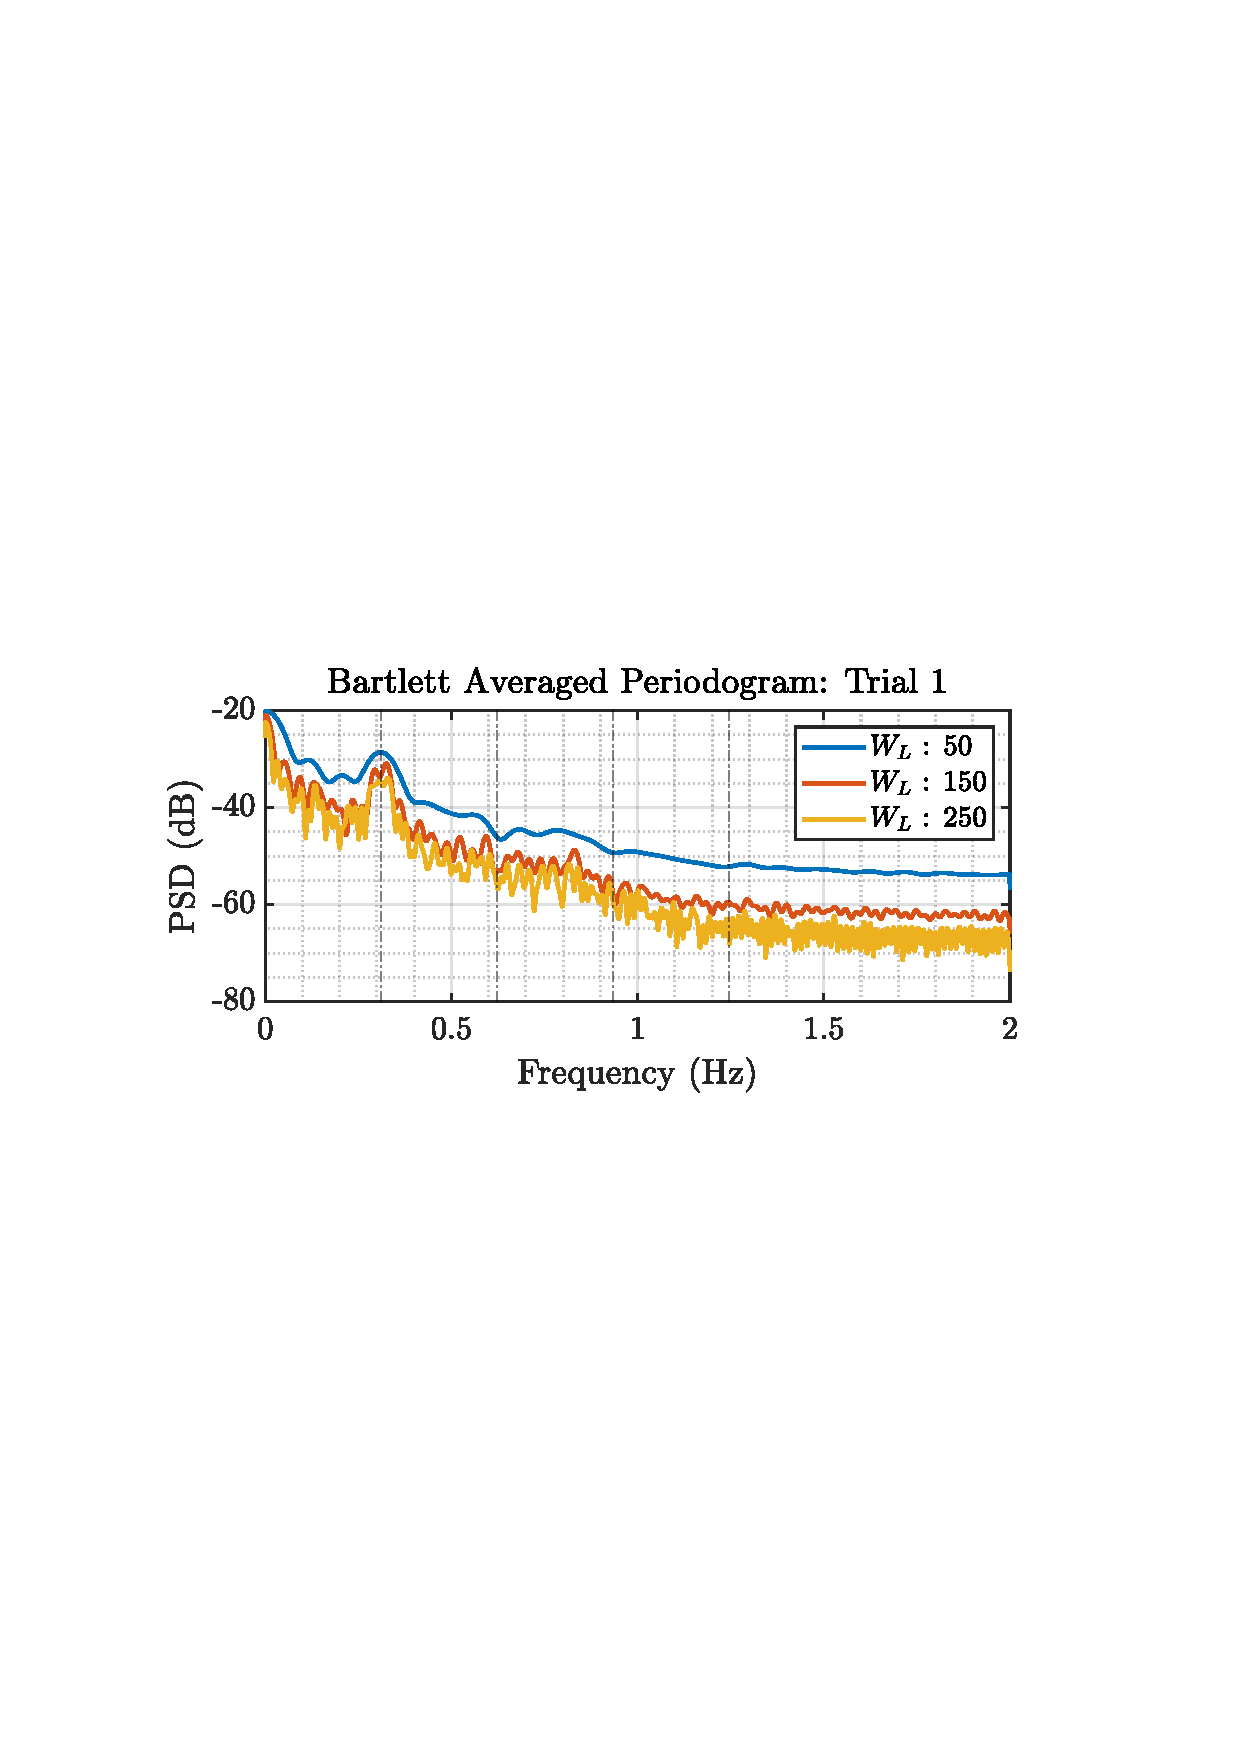
\includegraphics[trim={2.2cm 11cm 3.15cm  11.2cm}, clip, width=\textwidth]{../MATLAB/figures/q1_5a_fig04.pdf} 
		\end{subfigure}
		\begin{subfigure}{0.49\textwidth}
			\centering
			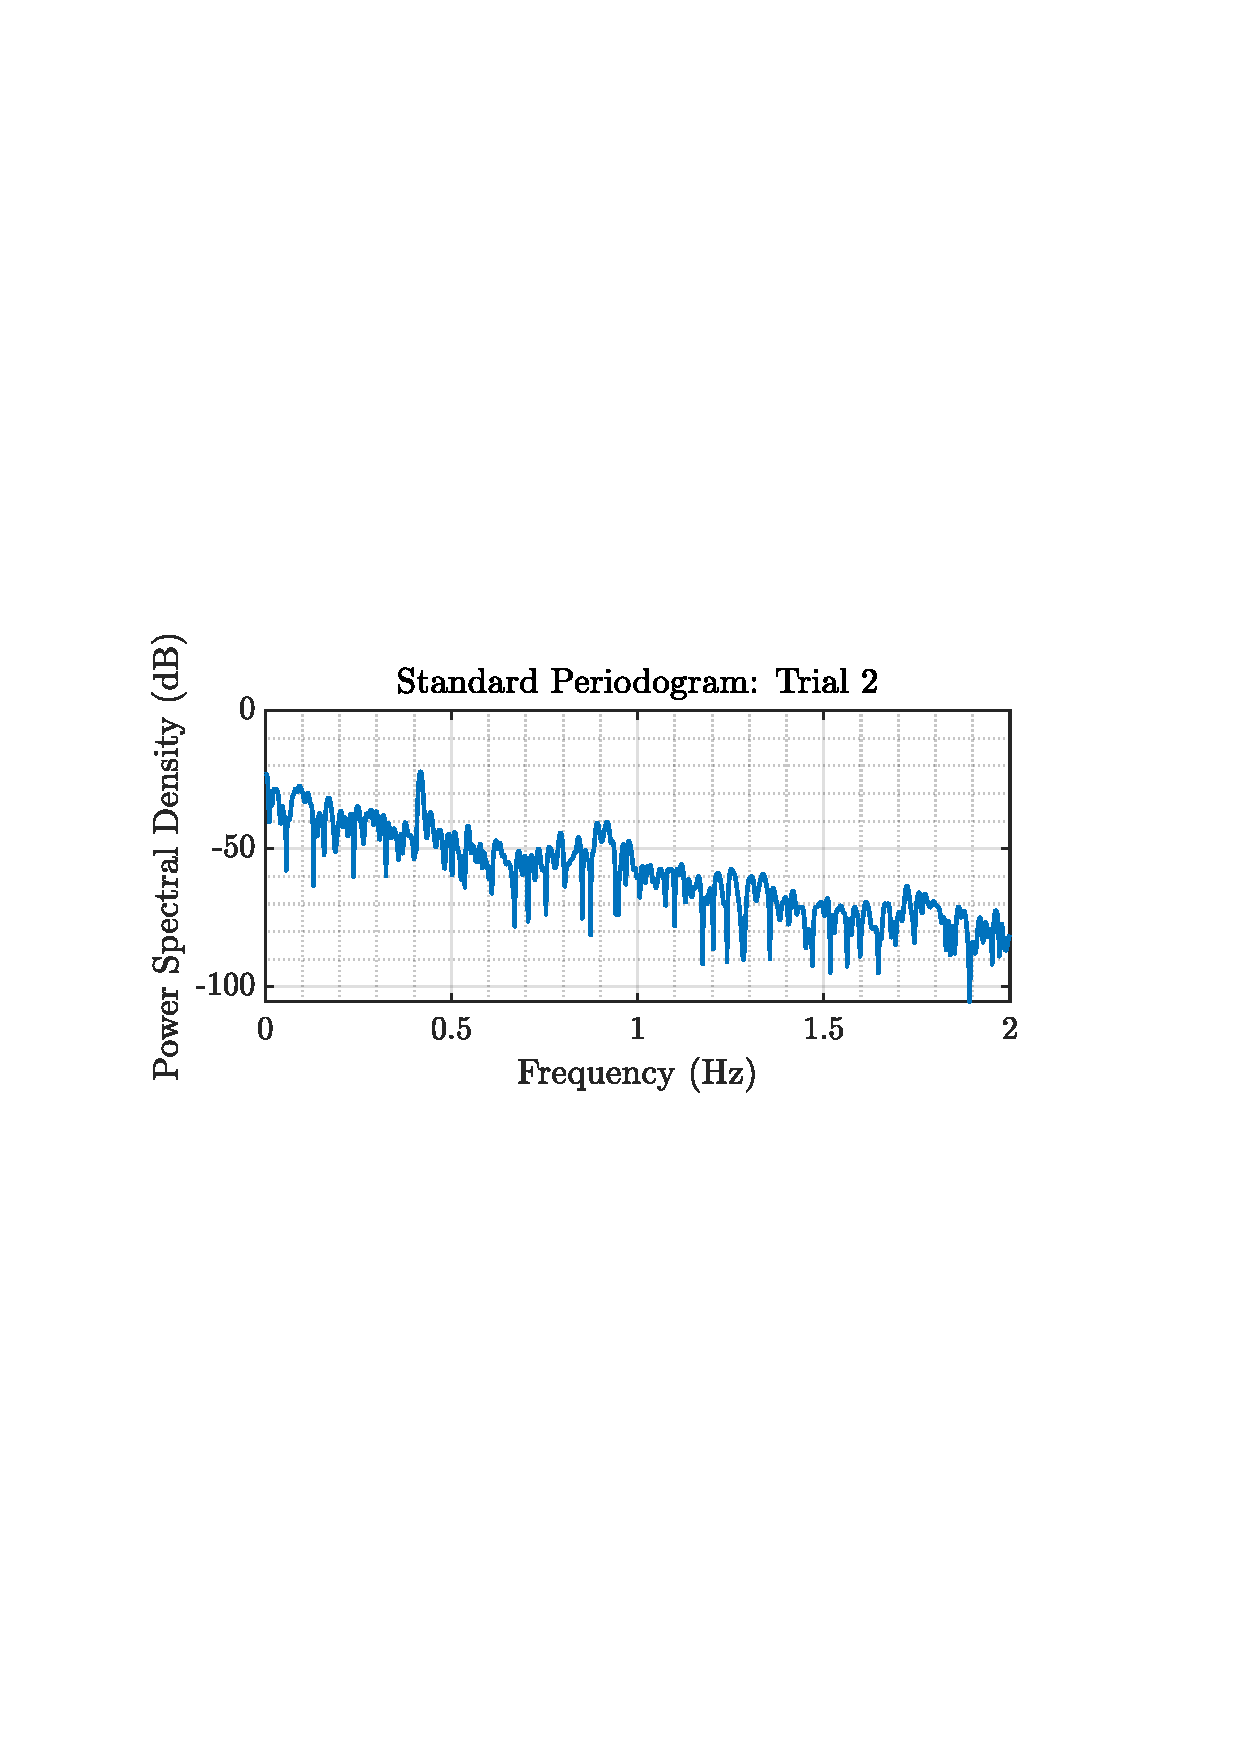
\includegraphics[trim={2.2cm 11cm 3.15cm  11.2cm}, clip, width=\textwidth]{../MATLAB/figures/q1_5a_fig02.pdf} 
		\end{subfigure}
		%		~ % forces onto the same row
		\begin{subfigure}{0.49\textwidth}
			\centering
			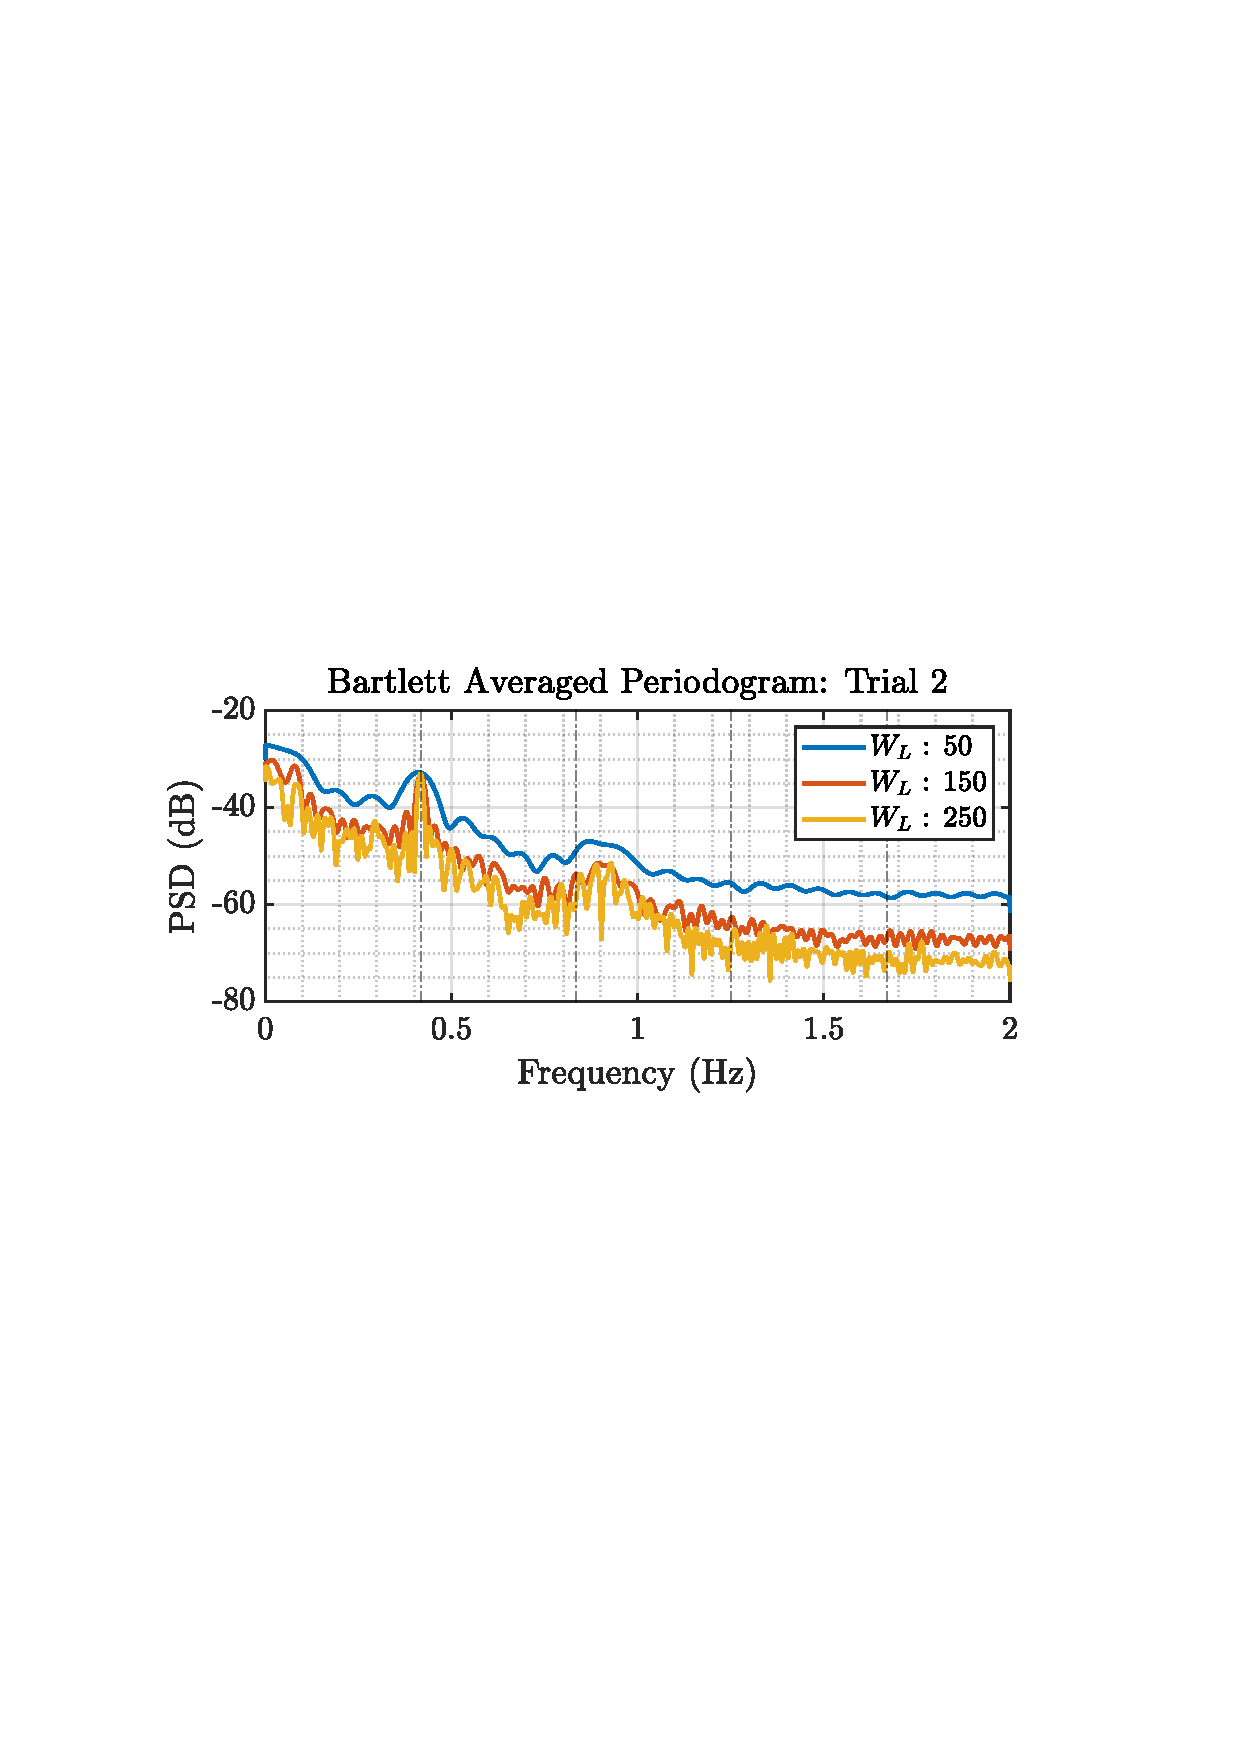
\includegraphics[trim={2.2cm 11cm 3.15cm  11.2cm}, clip, width=\textwidth]{../MATLAB/figures/q1_5a_fig05.pdf} 
		\end{subfigure}
		\begin{subfigure}{0.49\textwidth}
			\centering
			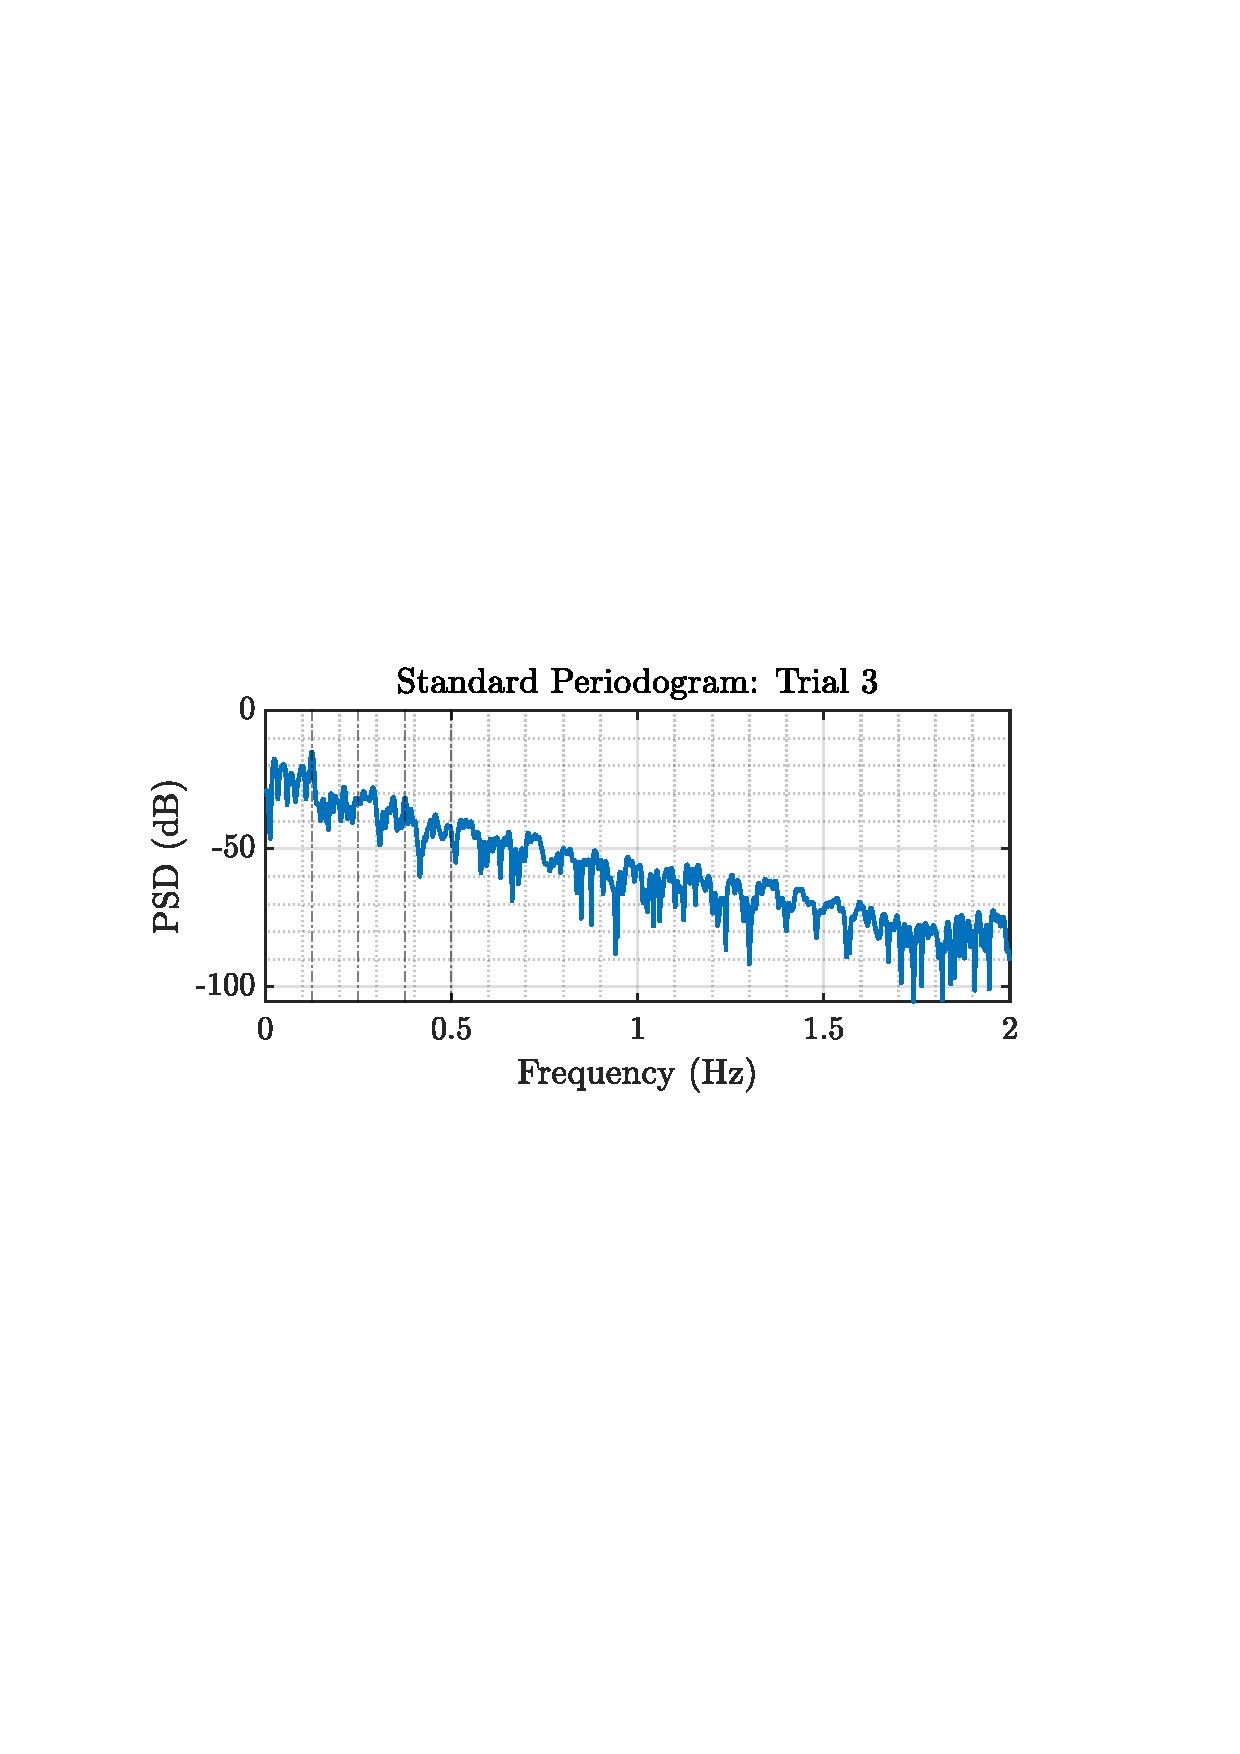
\includegraphics[trim={2.2cm 11.2cm 3.15cm  11.2cm}, clip, width=\textwidth]{../MATLAB/figures/q1_5a_fig03.pdf} 
		\end{subfigure}
		%		~ % forces onto the same row
		\begin{subfigure}{0.49\textwidth}
			\centering
			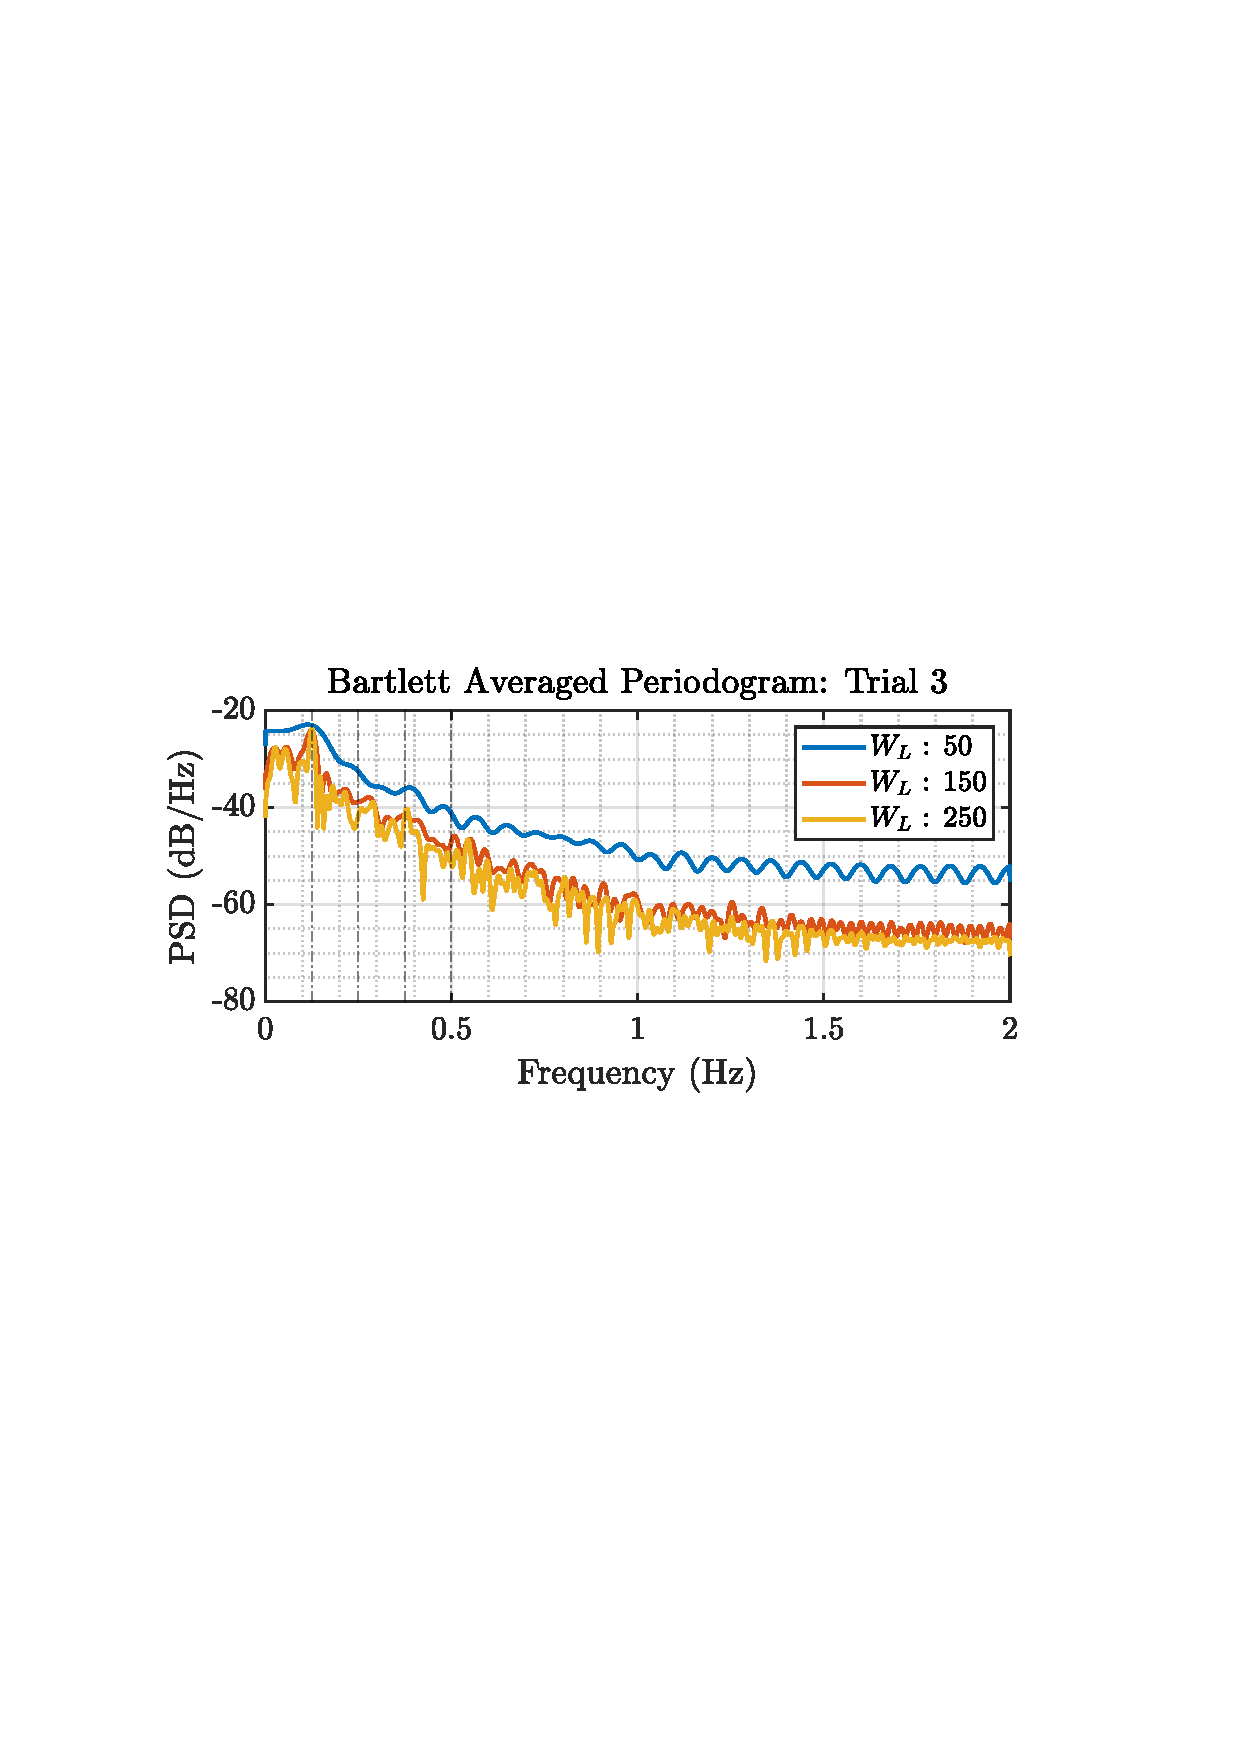
\includegraphics[trim={2.2cm 11.2cm 3.15cm  11.2cm}, clip, width=\textwidth]{../MATLAB/figures/q1_5a_fig06.pdf} 
		\end{subfigure}
		\captionsetup{justification=centering}
		\caption{Standard and Bartlett Average Periodograms. \\ 
				$W_L$ is the Window Length used. First 4 harmonics denoted by vertical black lines. Zero Padded Signal Length: $4096$.}
		\label{fig: 1-5a}
	\end{figure}

	\begin{table}[H]
		\centering
		\begin{tabular}{|c|c||c|}
			\hline
			\textbf{Breathing Type} & \textbf{Expected} (BPM) & \textbf{Observed Peak} (BPM) \\
			\hline
			\hline
			{Normal (Trial 1)} & $10-15$ & $0.31\times60\approx18.7$ \\
			\hline
			{Fast (Trial 2)} & $25$ & $0.41\times60\approx25$ \\
			\hline
			{Slow (Trial 3)} & $7.5$ & $0.125\times60=7.5$ \\
			\hline
		\end{tabular}
		\captionsetup{justification=centering}
		\caption{Breaths Per Minute (BPM), i.e. Observed Frequency $\times 60$, for all trials.}
		\label{tab: 1-5a}
	\end{table}


	\subsubsection{Analysis of the RRI PSD Estimates}
	
	Figure \ref{fig: 1-5a} shows us distinct peaks for each trial that somewhat agrees with the breathing expected. We note that harmonics are difficult to distinguish, despite the large zero padding of the signal. Table \ref{tab: 1-5a} highlights how the observed peaks align with the expected peaks.
	\pagebreak
	
	\subsubsection{AR PSD Estimate for the RRI Dataset}
	
%	\begin{wrapfigure}{r}{0.49\textwidth}
%		\vspace{-20pt}
%		\begin{centering}
%			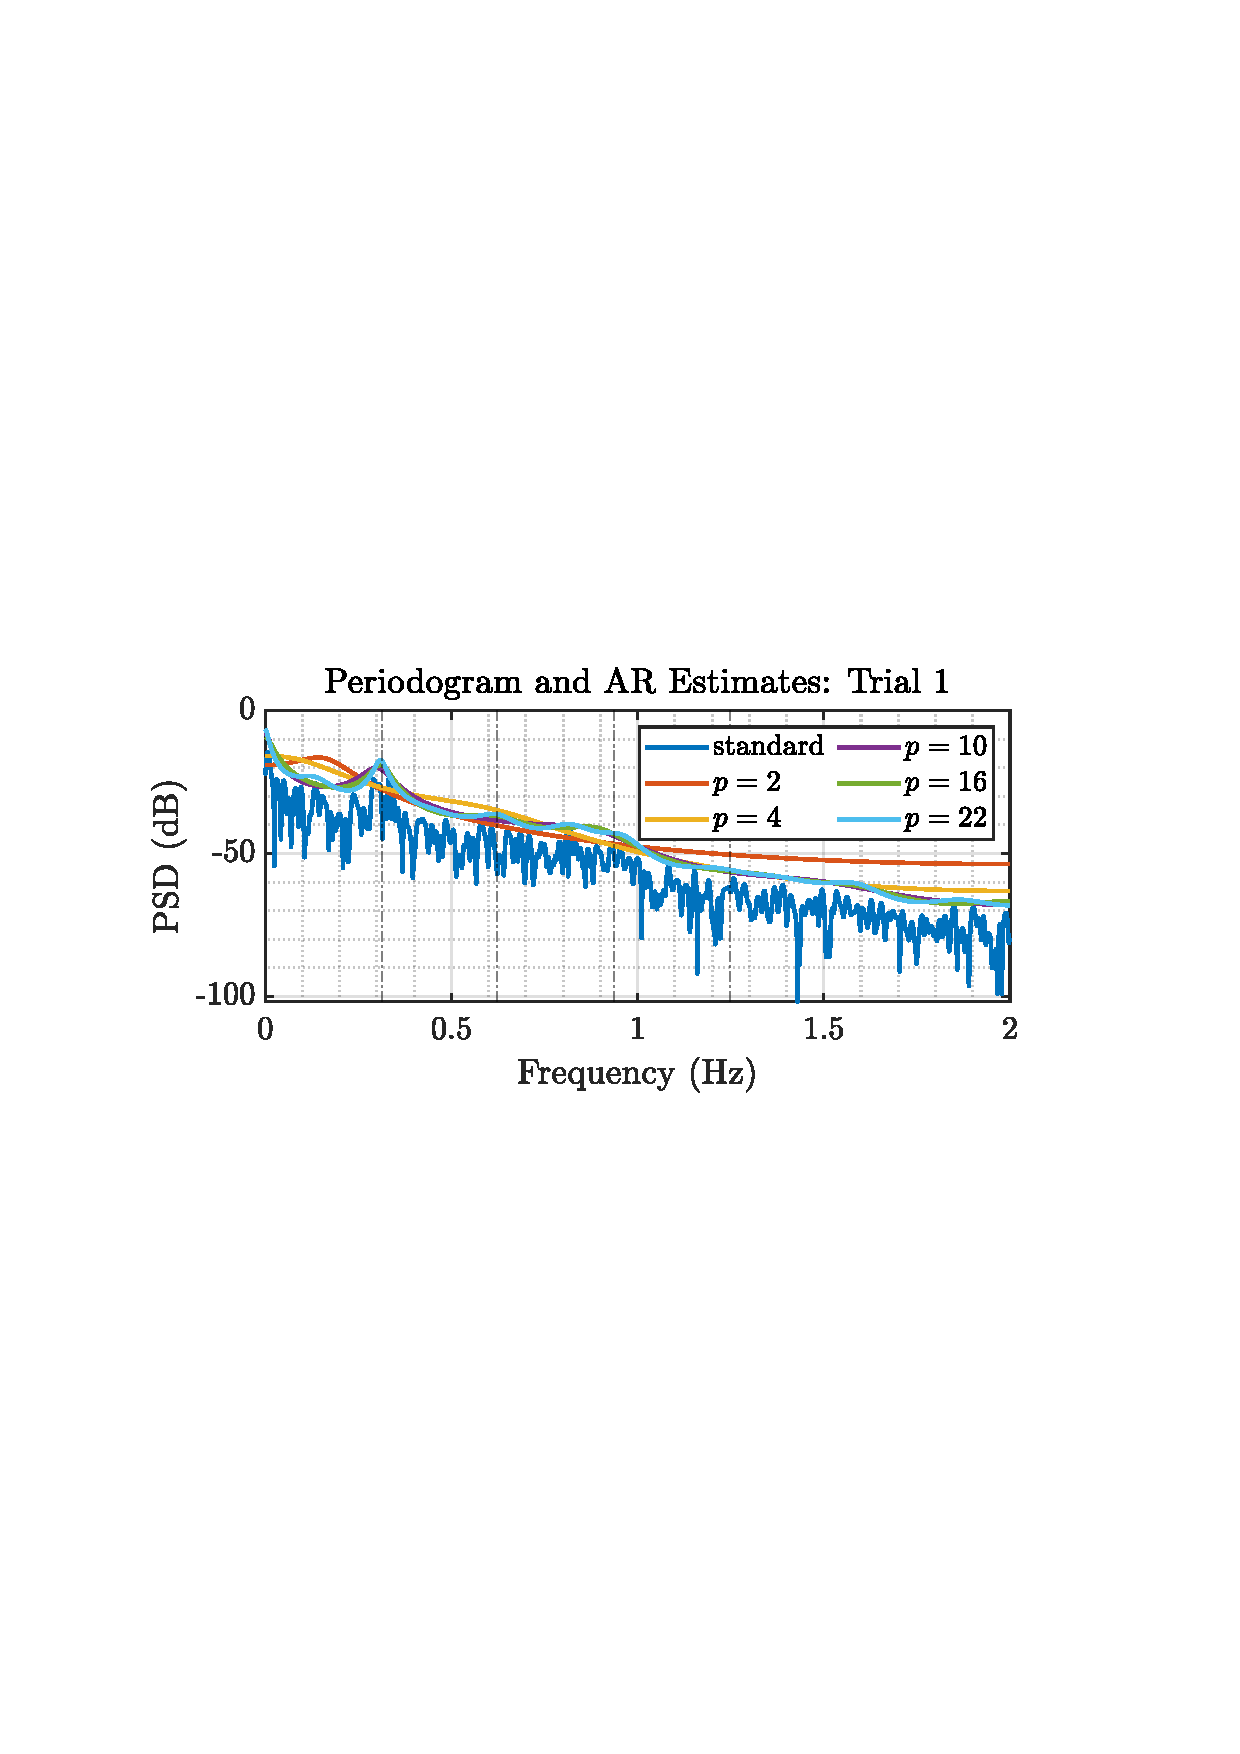
\includegraphics[trim={2.2cm 11.2cm 3.15cm  11.2cm}, clip, width=0.49\textwidth]{../MATLAB/figures/q1_5c_fig01.pdf} 
%		\end{centering}
%%		\vspace{-20pt}
%%		\vspace{-10pt}
%		\begin{centering}
%			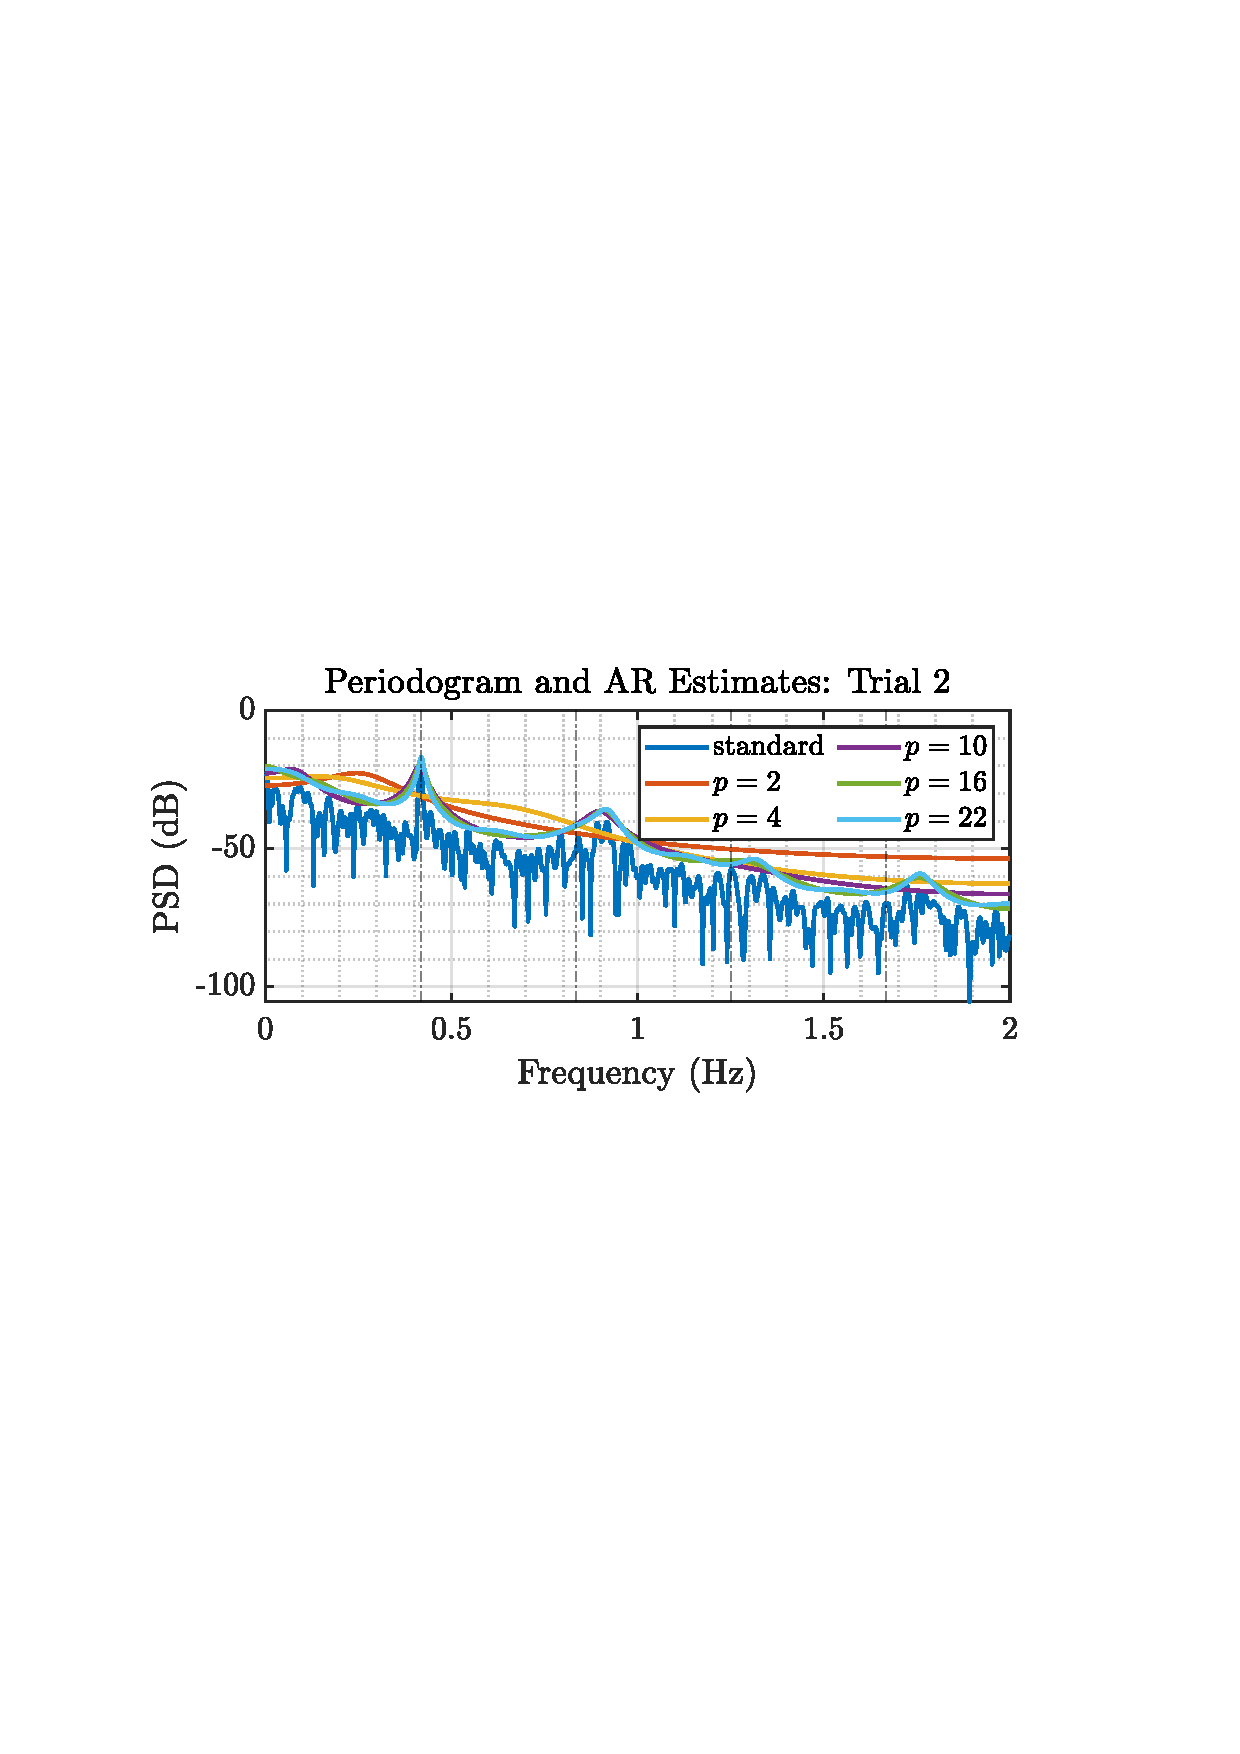
\includegraphics[trim={2.2cm 11.2cm 3.15cm  11.2cm}, clip, width=0.49\textwidth]{../MATLAB/figures/q1_5c_fig02.pdf} 
%		\end{centering}
%%		\vspace{-20pt}
%%		\vspace{-10pt}
%		\begin{centering}
%			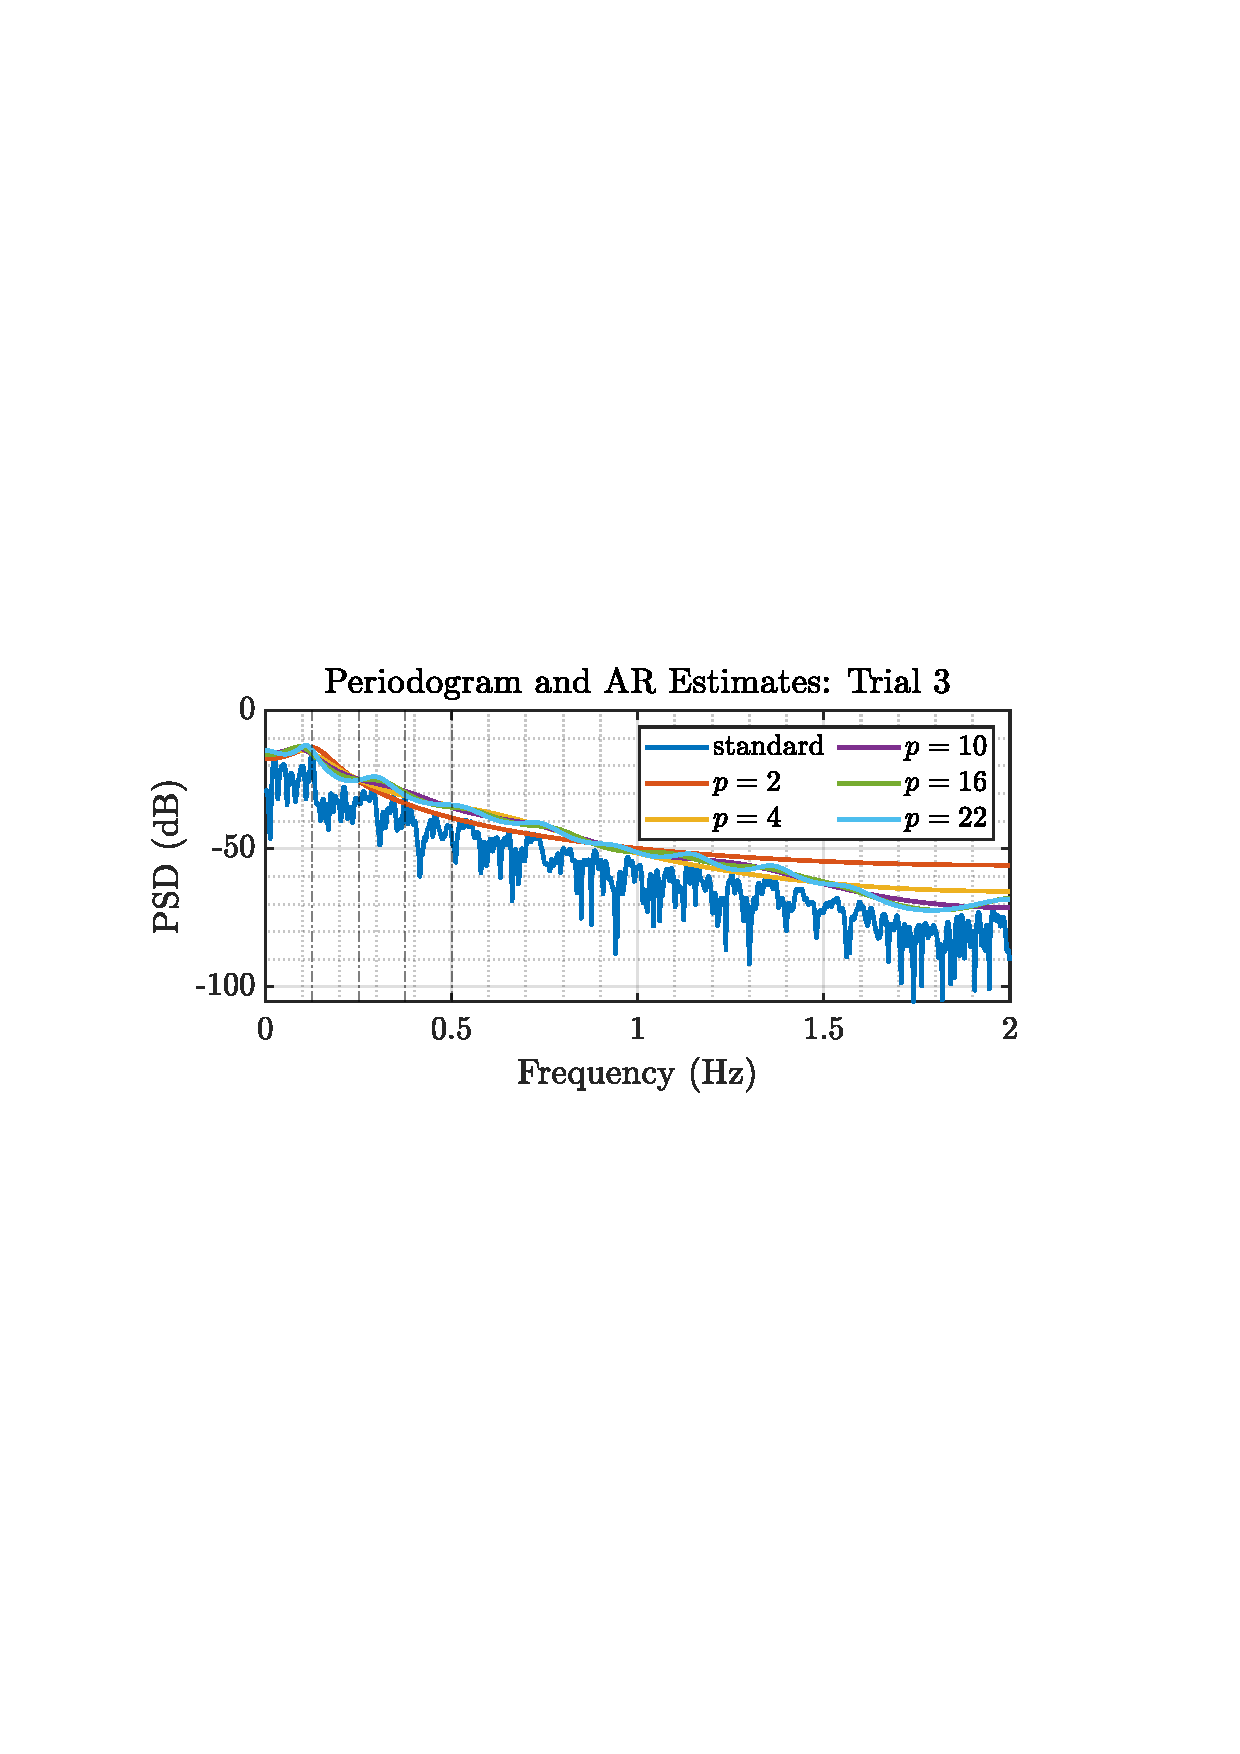
\includegraphics[trim={2.2cm 11.2cm 3.15cm  11.2cm}, clip, width=0.49\textwidth]{../MATLAB/figures/q1_5c_fig03.pdf} 
%		\end{centering}
%%		\vspace{-20pt}
%		\captionsetup{justification=centering}
%		\caption{AR Estimate Periodograms. \\ $p$ is the model order.}
%		\label{fig: 1-5c}
%%		\vspace{-10pt}
%	\end{wrapfigure}

		\begin{figure}[H]
			\begin{subfigure}{0.49\textwidth}
				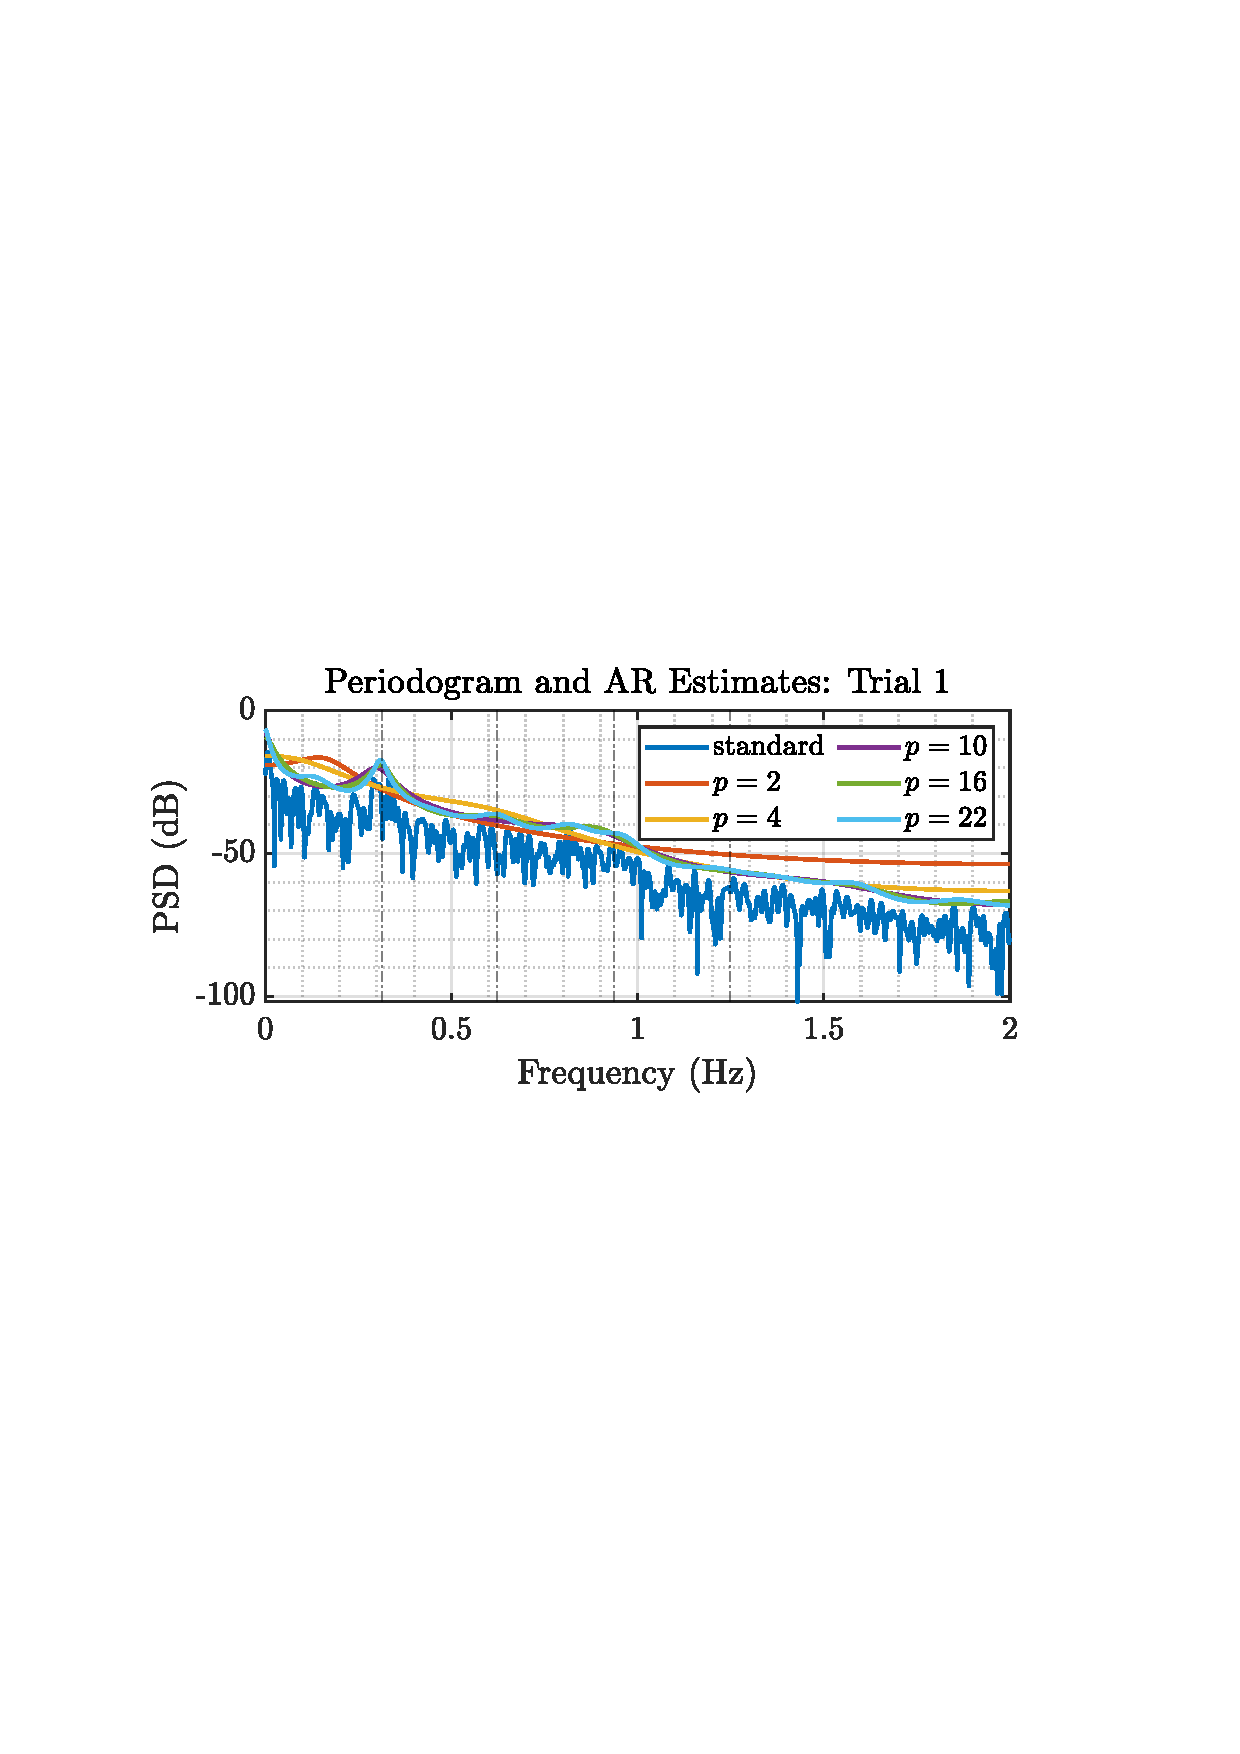
\includegraphics[trim={2.2cm 11.2cm 3.15cm  11.2cm}, clip, width=\textwidth]{../MATLAB/figures/q1_5c_fig01.pdf} 
				\caption{}
			\end{subfigure}
			\begin{subfigure}{0.49\textwidth}
				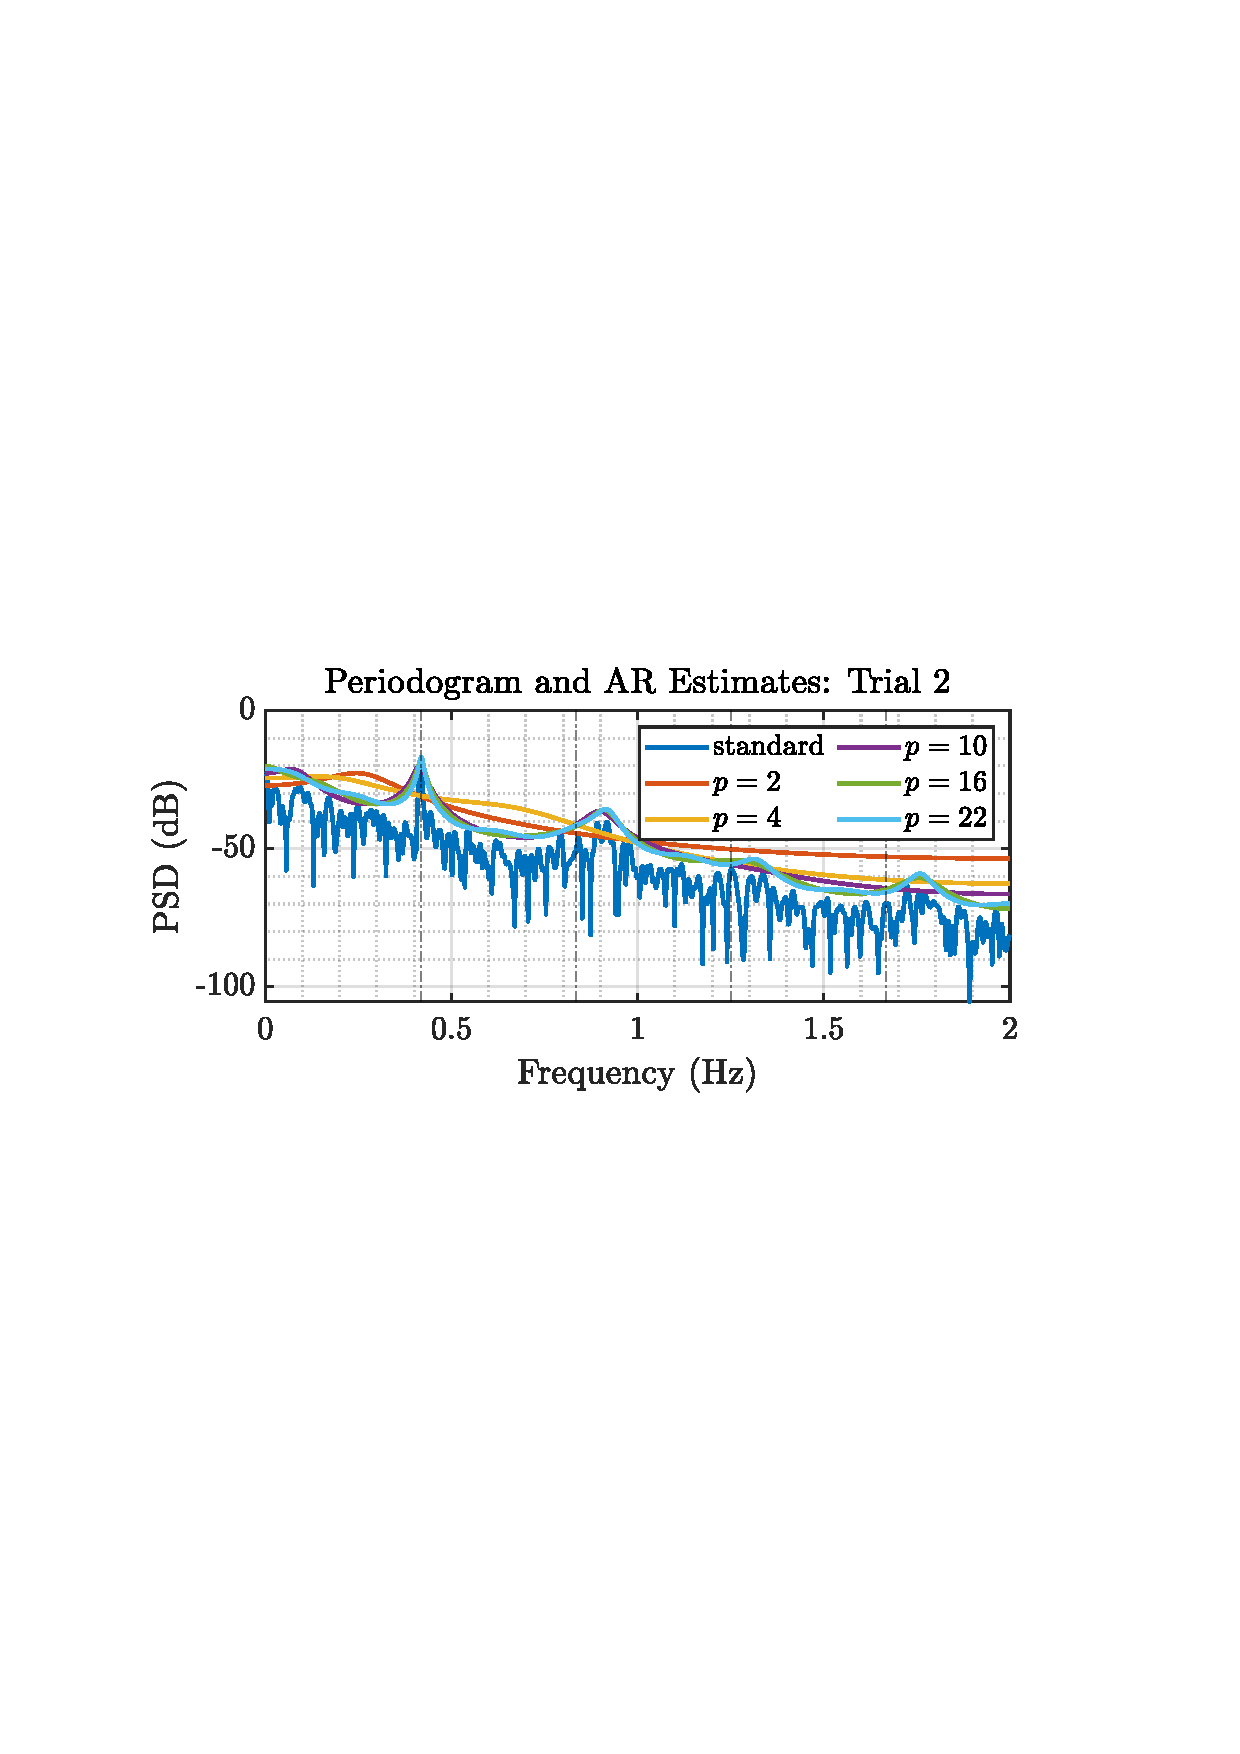
\includegraphics[trim={2.2cm 11.2cm 3.15cm  11.2cm}, clip, width=\textwidth]{../MATLAB/figures/q1_5c_fig02.pdf} 
				\caption{}
			\end{subfigure}%
%			\hspace*{0.25\textwidth}
%			\begin{subfigure}{0.49\textwidth}
%				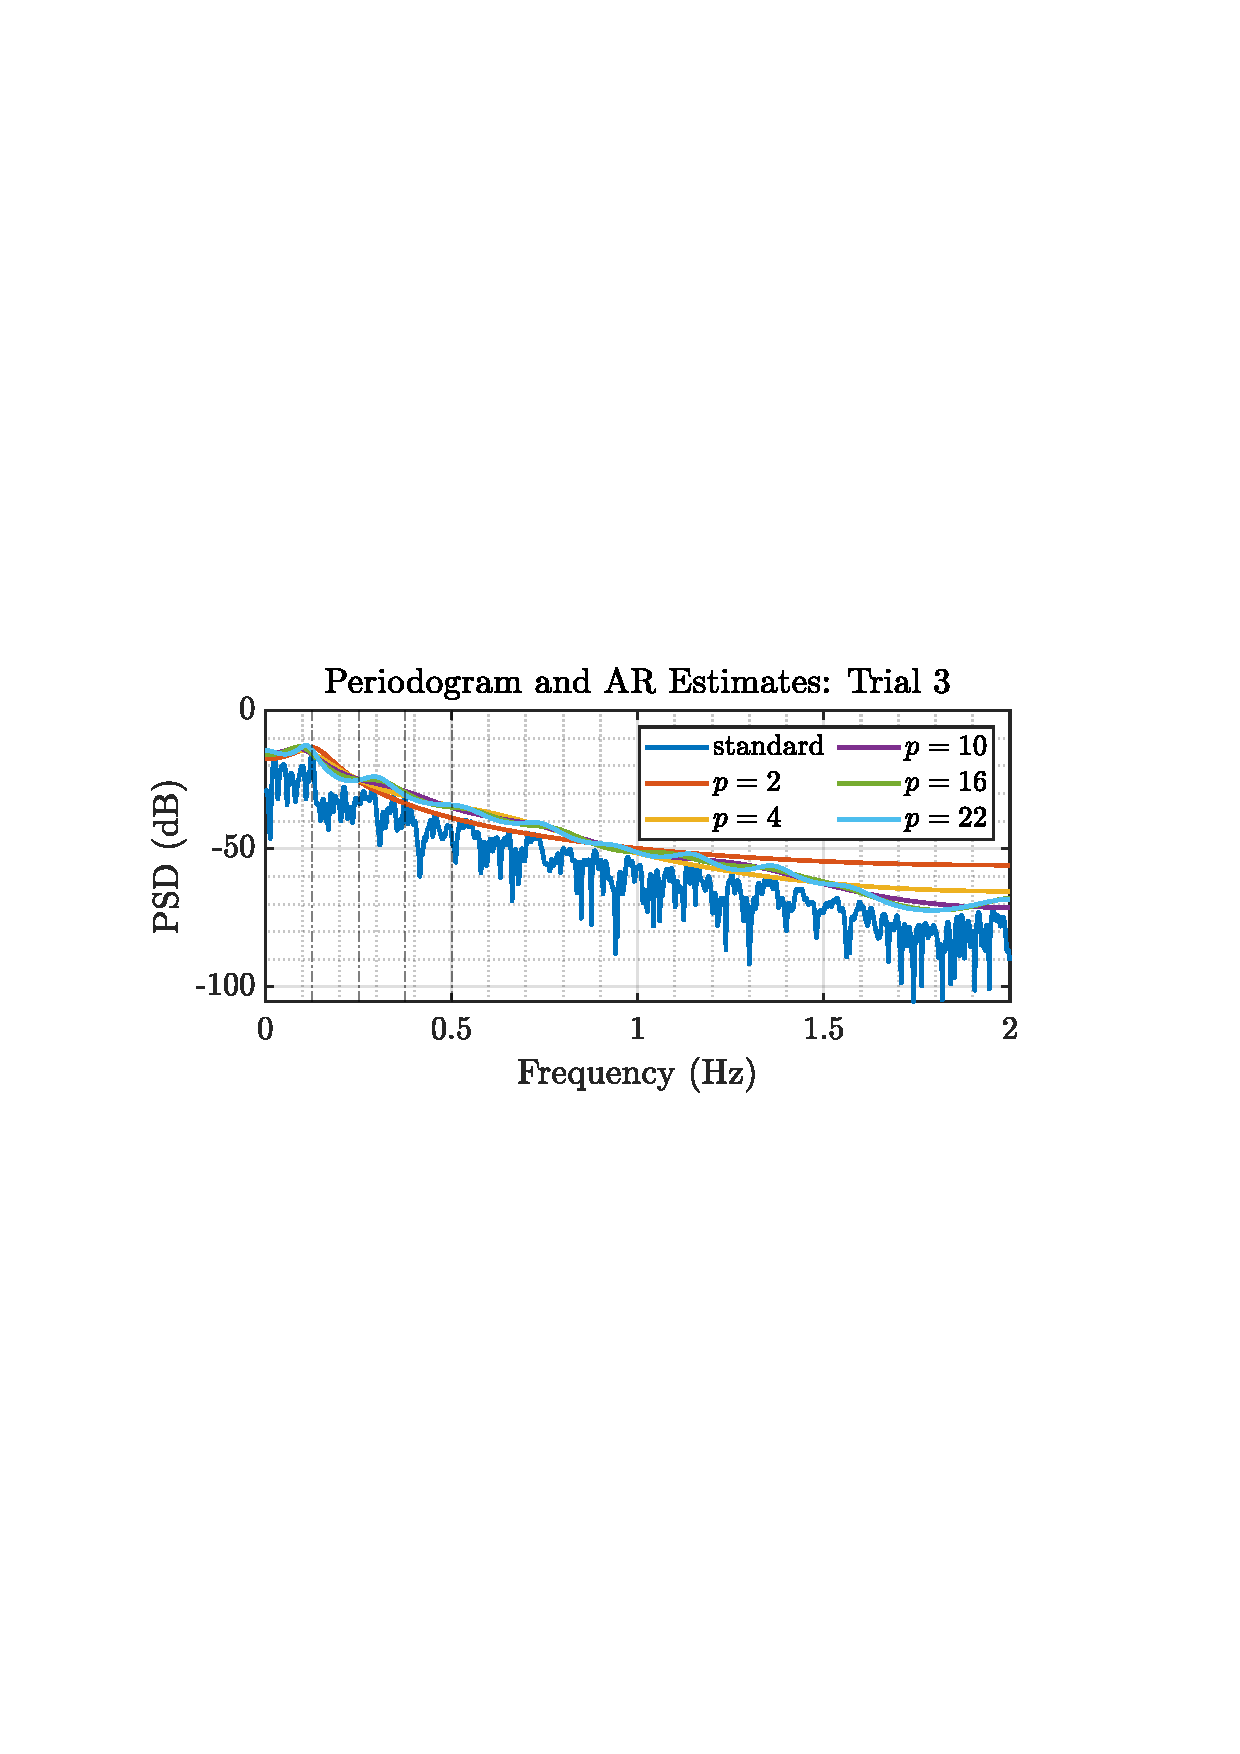
\includegraphics[trim={2.2cm 11.2cm 3.15cm  11.2cm}, clip, width=\textwidth]{../MATLAB/figures/q1_5c_fig03.pdf} 
%			\end{subfigure}
%			\captionsetup{justification=centering}
%			\caption{AR Estimate Periodograms. \\ $p$ is the model order.}
%			\label{fig: 1-5c}
			%		\vspace{-10pt}
			
			\begin{minipage}{0.46\textwidth}
				The AR spectral estimate in Figure \ref{fig: 1-5c} correctly identified the peak from models of order $p\gtrapprox10$. We note that the estimate resembles a smooth envelope over our PSD and correctly identifies clear peaks in the standard PSD at $p=10$. We also can see for higher order models that there are move fluctuations as the model starts to overfit for the input data's natural noisiness. \\
			\end{minipage}% 
			\begin{minipage}{0.04\textwidth}
				\hspace*{0.04\textwidth}
			\end{minipage}% 
			\begin{minipage}{0.49\textwidth}
				\begin{subfigure}{\textwidth}
					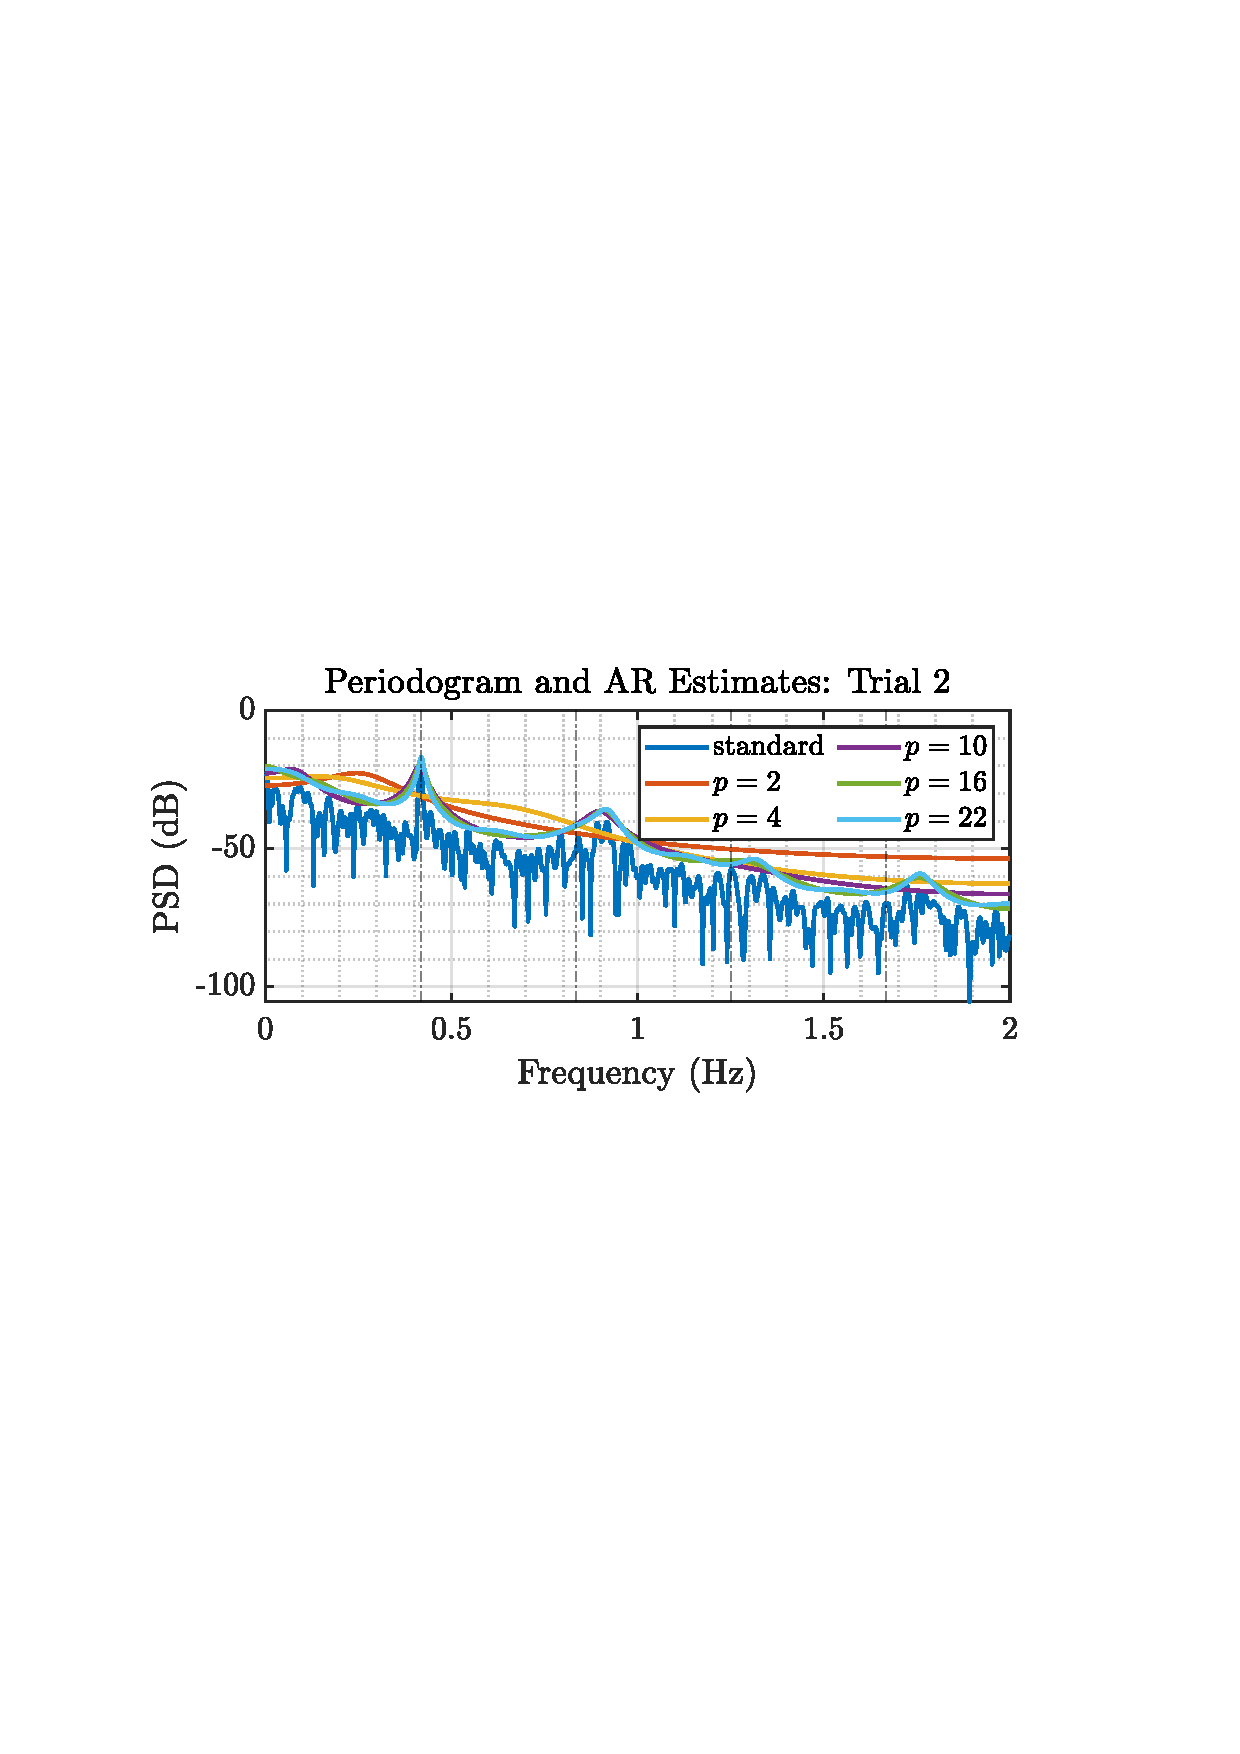
\includegraphics[trim={2.2cm 11.2cm 3.15cm  11.2cm}, clip, width=\textwidth]{../MATLAB/figures/q1_5c_fig02.pdf} 
					\caption{}
				\end{subfigure}%
%				\centering
%				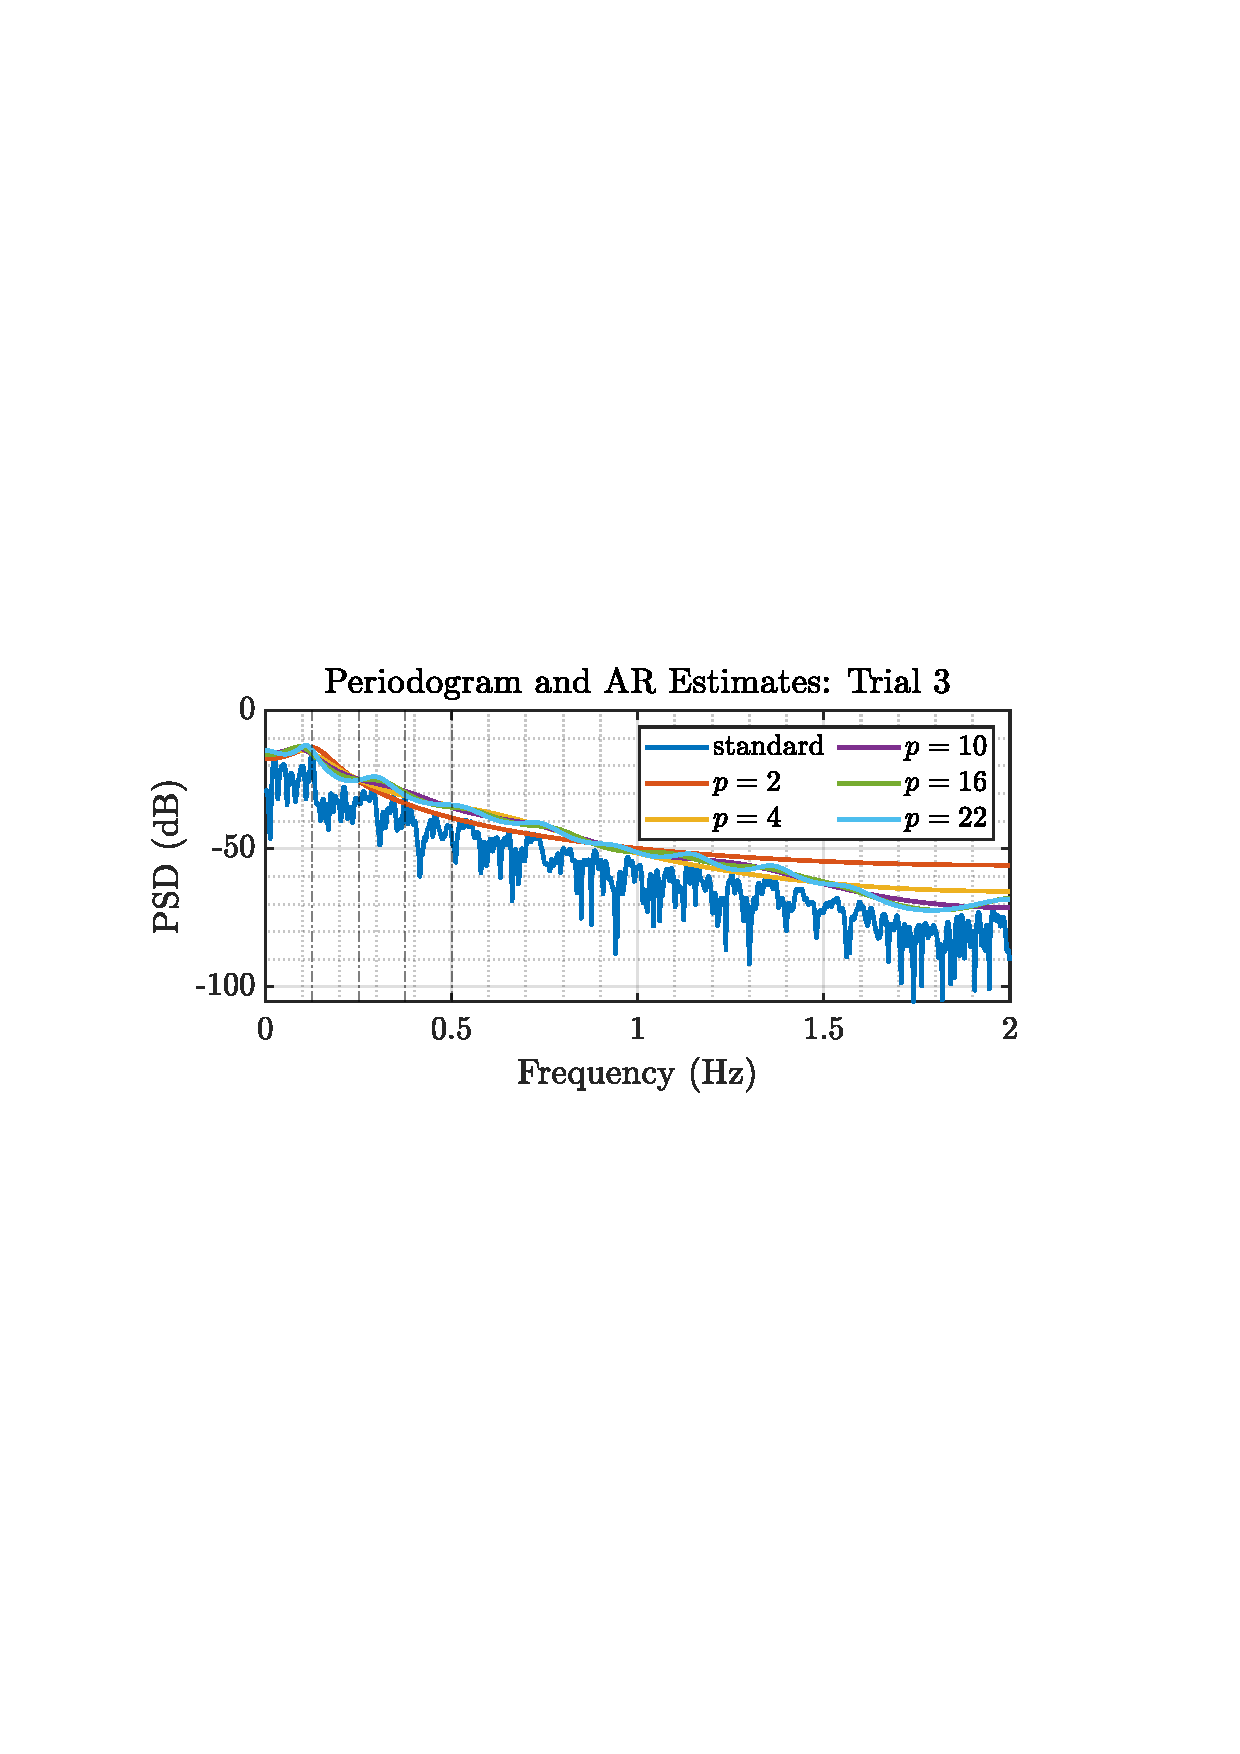
\includegraphics[trim={2.2cm 11.2cm 3.15cm  11.2cm}, clip, width=\textwidth]{../MATLAB/figures/q1_5c_fig03.pdf} 
				\captionsetup{justification=centering}
				\captionof{figure}{AR Estimate Periodograms. \\ $p$ is the model order.}
				\label{fig: 1-5c}
			\end{minipage}%
		\end{figure}
	

%	\pagebreak
	
	
	\subsection{Robust Regression} \label{sec: 1-6-robust-regression} 
	 	\subsubsection{Single Value Decomposition (SVD)}
			\begin{figure}[H]
				\centering
				\begin{subfigure}{0.49\textwidth}
					\centering
					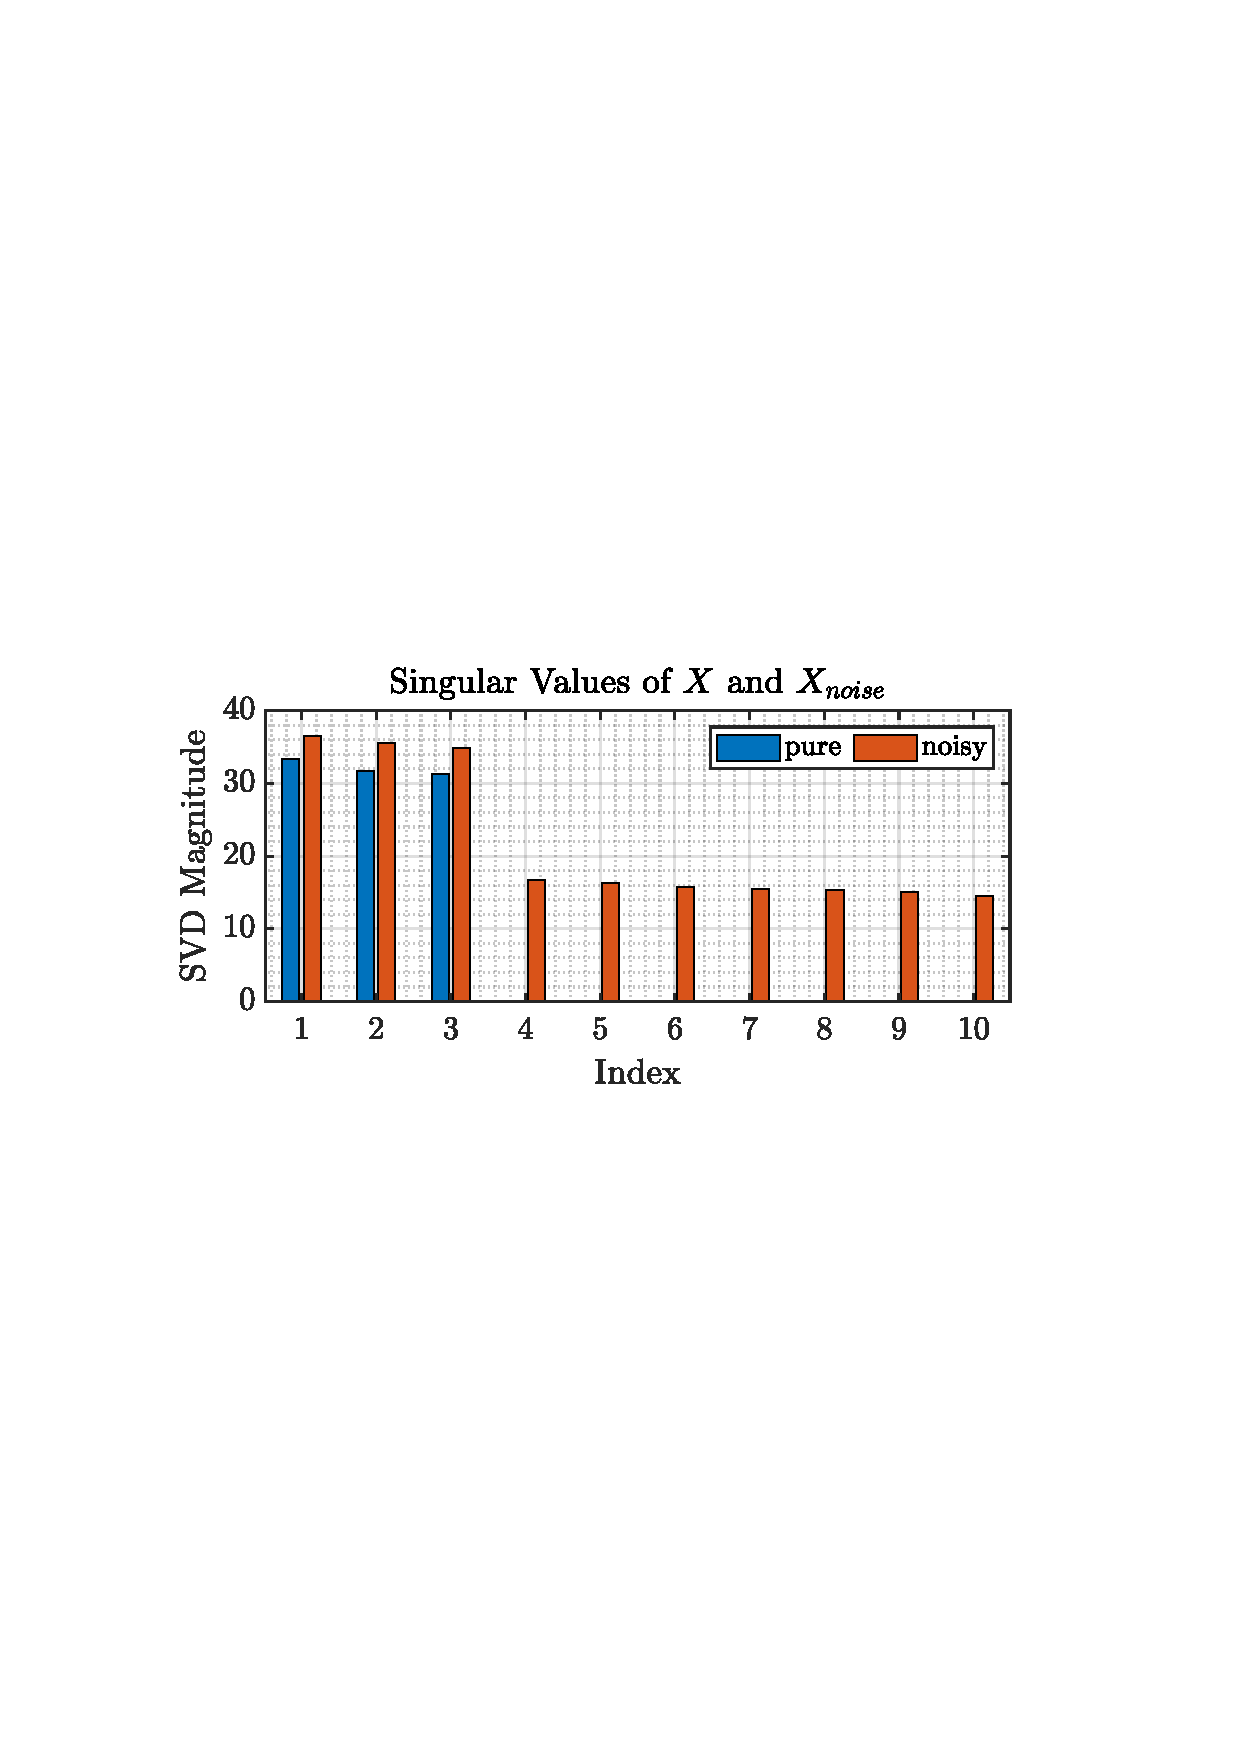
\includegraphics[trim={2.2cm 11.2cm 3.15cm  11.2cm}, clip, width=\textwidth]{../MATLAB/figures/q1_6a_fig01.pdf} 
					\captionsetup{justification=centering}
					\caption{SVD}
				\end{subfigure}
				%		~ % forces onto the same row
				\begin{subfigure}{0.49\textwidth}
					\centering
					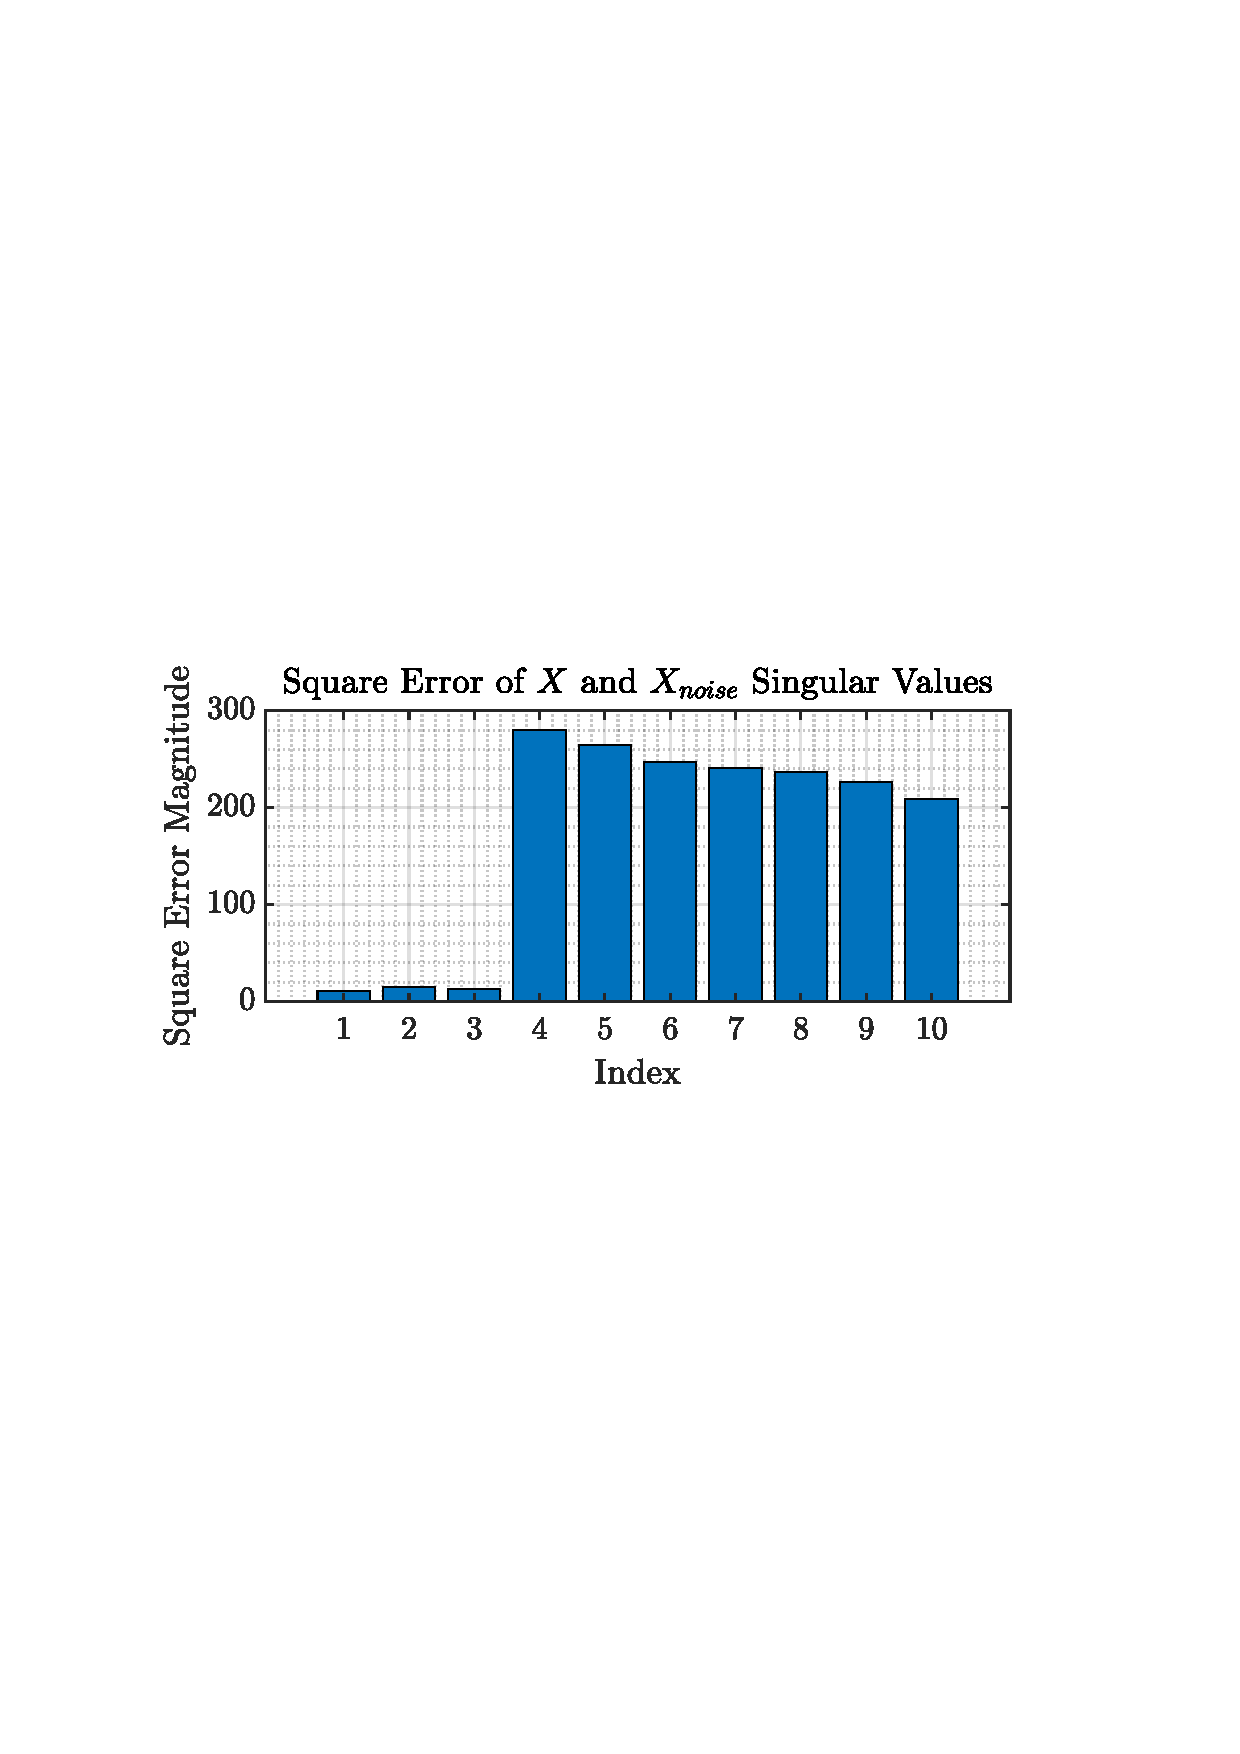
\includegraphics[trim={2.2cm 11.2cm 3.15cm  11.2cm}, clip, width=\textwidth]{../MATLAB/figures/q1_6a_fig02.pdf} 
					\captionsetup{justification=centering}
					\caption{Square Error}
				\end{subfigure}
				\captionsetup{justification=centering}
				\caption{}
				\label{fig: 1-6a}
			\end{figure}
		
		
		
			The rank of the input data would be indicated when the SVD Error increases or the non-zero SVD values end (for pure data) - hence the data is of rank 3. \\
			Noise makes the SVD magnitude non-zero where we expect it to be zero for the pure input. Hence, in the real world where we would not have the pure dataset we would need to purely look at Figure \ref{fig: 1-6a} (a), if the SVD magnitude of the noise was comparable to that of the signal we would have difficulty establishing a criteria to distinguish signal and noise subspaces from the SVD method. \\
	 
	% 	\pagebreak
	 	
	 	\subsubsection{Low Rank Approximation Error}
		 	\begin{minipage}[b]{0.49\textwidth}
			By looking at the mean square error between the pure signal and the low-rank approximation of the noise, Figure \ref{fig: 1-6b}, we note that the minimum error is when the low-rank approximation matches that of the pure data.
			\end{minipage}% 
			\begin{minipage}{0.04\textwidth}
				\hspace*{0.04\textwidth}
			\end{minipage}% 
			\begin{minipage}{0.49\textwidth}
				\centering
				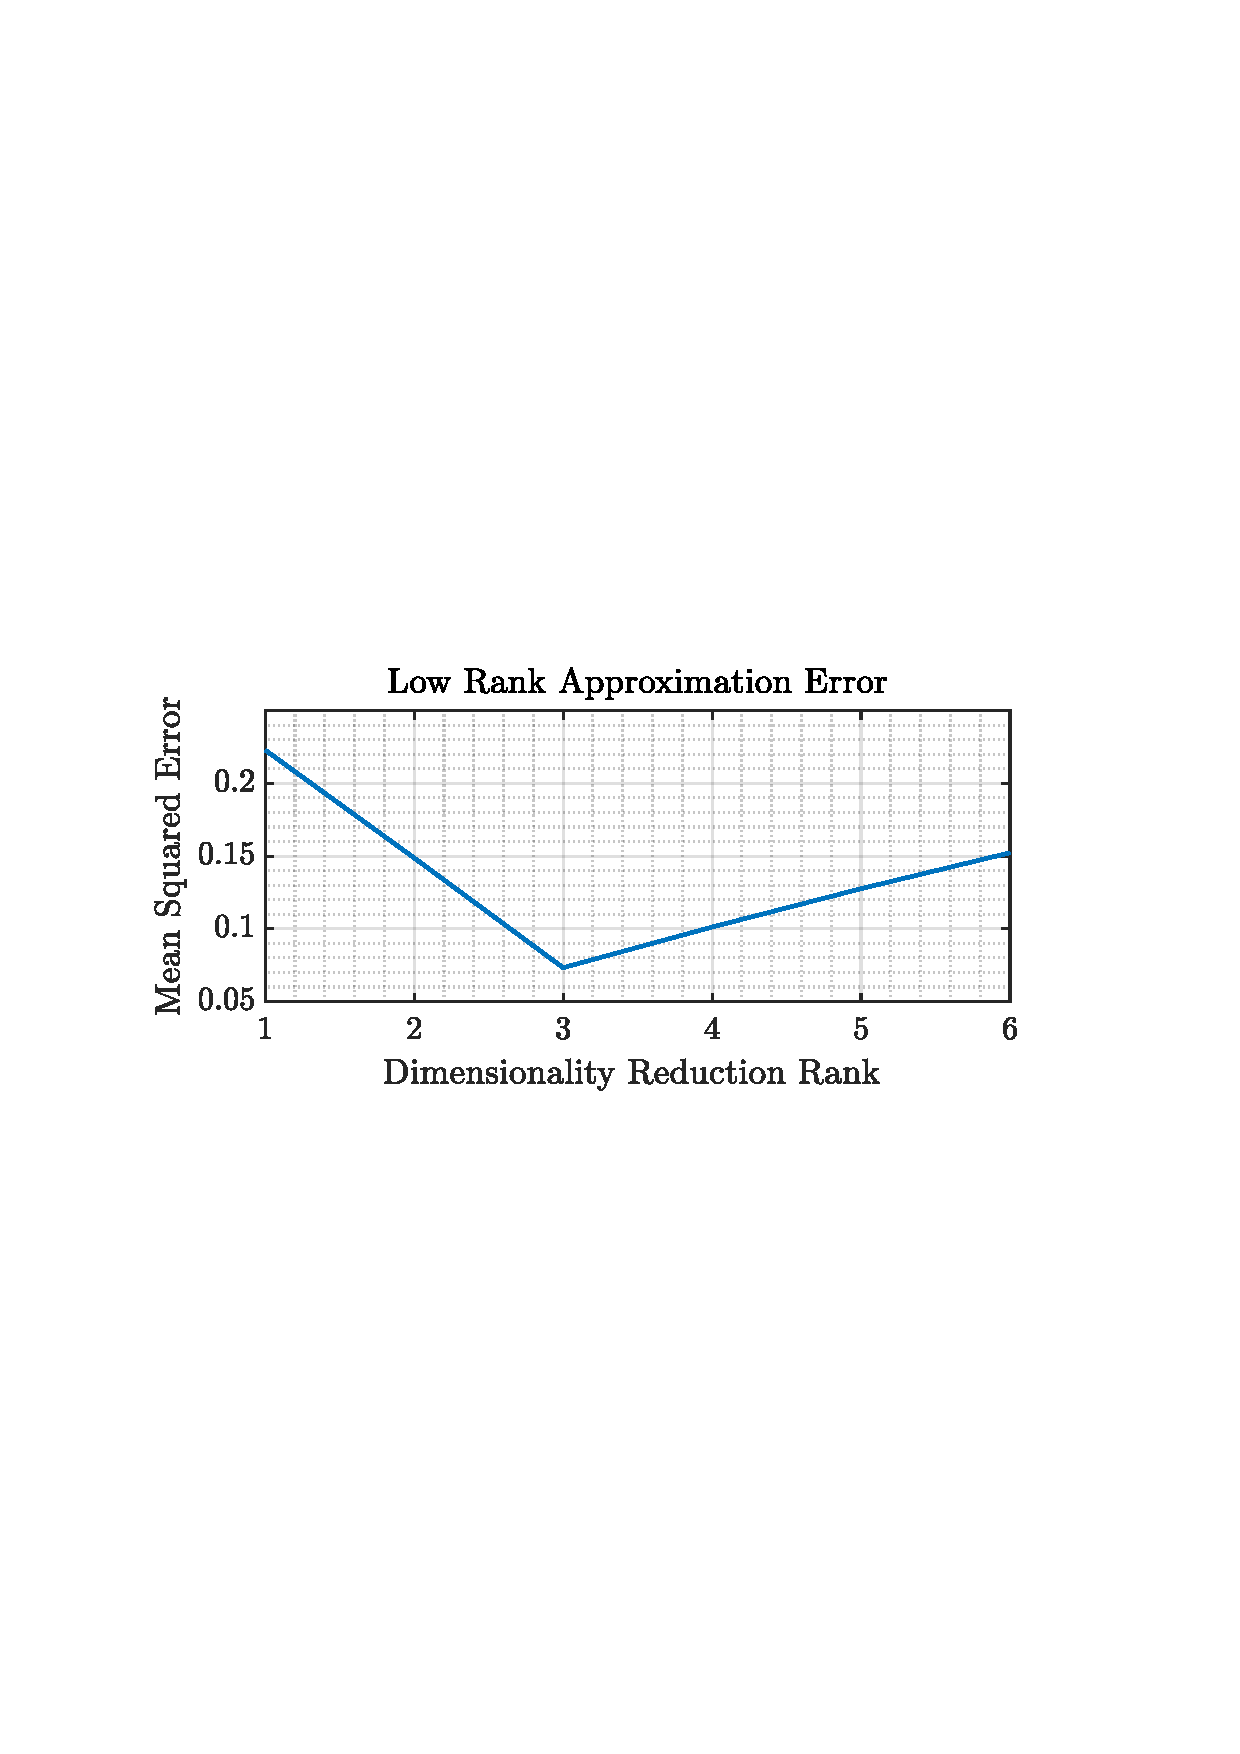
\includegraphics[trim={2.2cm 11.2cm 3.15cm  11.2cm}, clip, width=\textwidth]{../MATLAB/figures/q1_6b_fig01.pdf} 
				\captionsetup{justification=centering}
				\captionof{figure}{Effect of Changing Rank on the Approximation Error}
				\label{fig: 1-6b}
			\end{minipage}%
	
	 
	 	\subsubsection{Ordinary Least Squares (OLS) \& Principle Component Regression (PCR)  Estimate Errors}
	 	
		 	\begin{figure}[H]
		 		\centering
		 		\begin{subfigure}{0.49\textwidth}
		 			\centering
		 			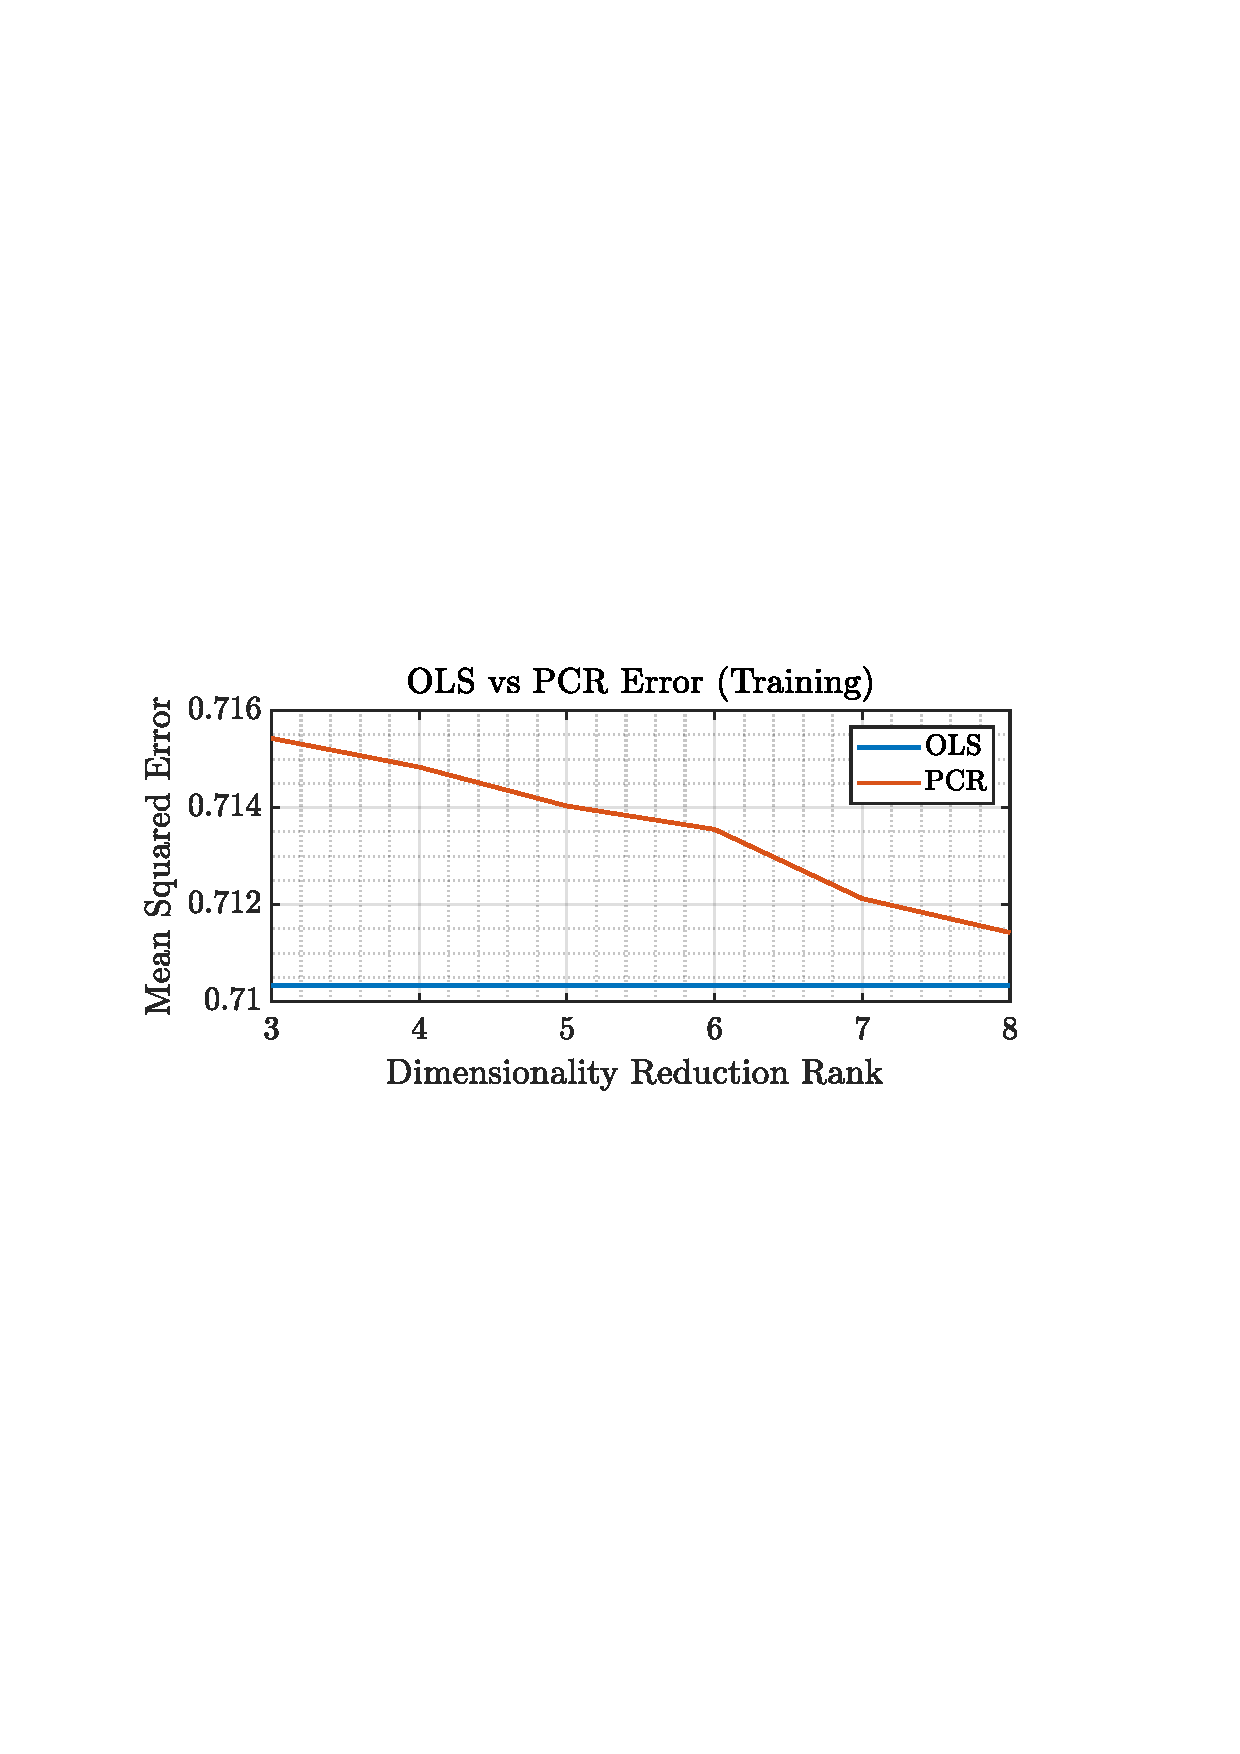
\includegraphics[trim={2.2cm 11.2cm 3.15cm  11.2cm}, clip, width=\textwidth]{../MATLAB/figures/q1_6c_fig01.pdf} 
		 			\captionsetup{justification=centering}
		 			\caption{Training Dataset Error}
		 		\end{subfigure}
		 		%		~ % forces onto the same row
		 		\begin{subfigure}{0.49\textwidth}
		 			\centering
		 			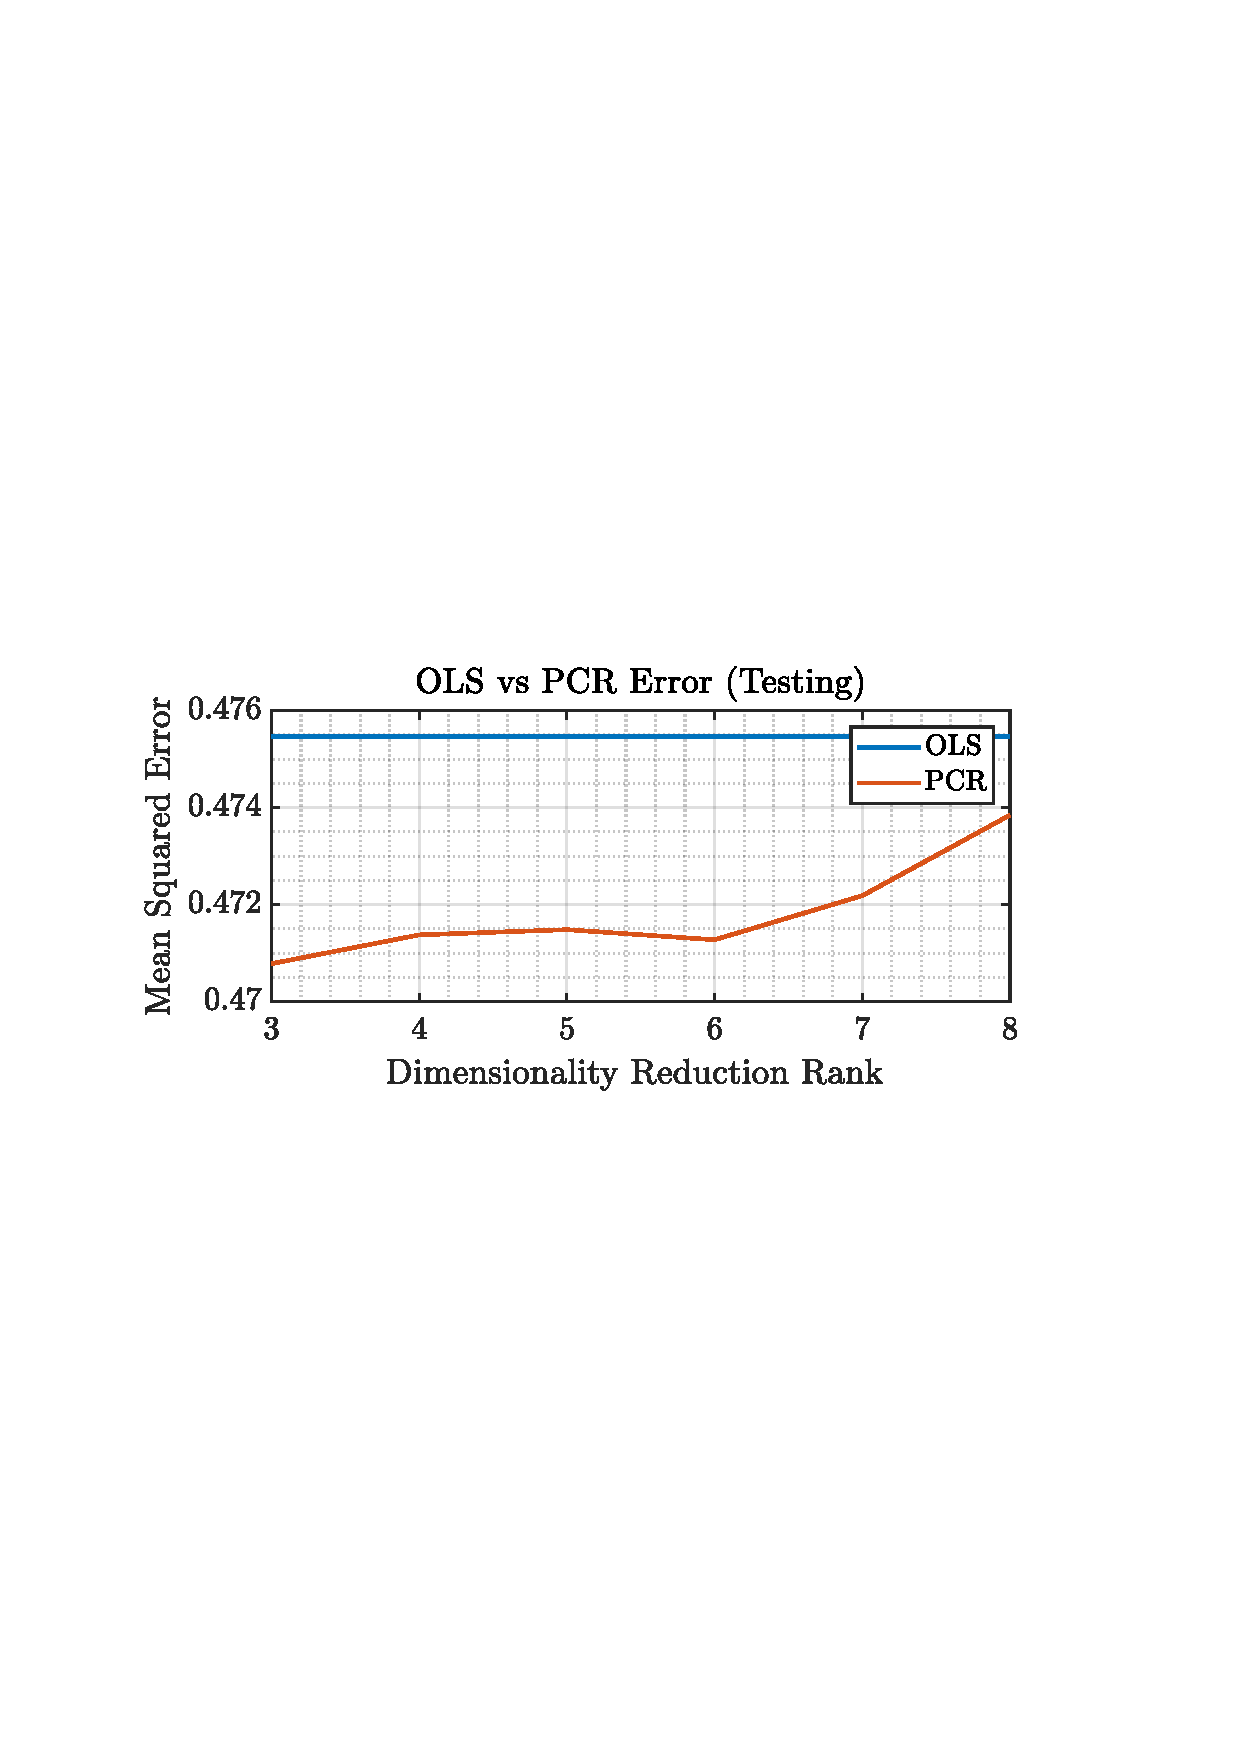
\includegraphics[trim={2.2cm 11.2cm 3.15cm  11.2cm}, clip, width=\textwidth]{../MATLAB/figures/q1_6c_fig02.pdf} 
		 			\captionsetup{justification=centering}
		 			\caption{Testing Dataset Error}
		 		\end{subfigure}
		 		\captionsetup{justification=centering}
		 		\caption{Comparison of Errors in the Training and Testing Datasets}
		 		\label{fig: 1-6c}
		 	\end{figure}
		 
		 	In both datasets we see that at the true model order the differences are tiny, in the training dataset we see that PCR underperforms by $0.85\%$, while in the testing dataset PCR outperforms by $1.05\%$. We can also note that decreasing the PCR model order further than the true model order, improves performance in the Training dataset but reduces performance in the Testing dataset.
		
		
	 	\subsubsection{Ordinary Least Squares (OLS) \& Principle Component Regression (PCR)  Estimate Errors - Part 2}
	 	\begin{minipage}{0.49\textwidth}
	 		Again if we look at the true model order, Figure \ref{fig: 1-6d}, PCR outperforms OLS by $0.79\%$. We note how further reduction in dimensionality decreases the performance of PCR. In regard to effectiveness of each scheme, if the model order is unknown and cannot be approximated accurately, OLS is a safer choice, however best performance - although marginal - can be achieved if the model order is known and PCR is implemented.
	 	\end{minipage}% 
		 \begin{minipage}{0.04\textwidth}
		 	  \hspace*{0.04\textwidth}
		 \end{minipage}% 
	 	\begin{minipage}{0.49\textwidth}
			\centering
	 		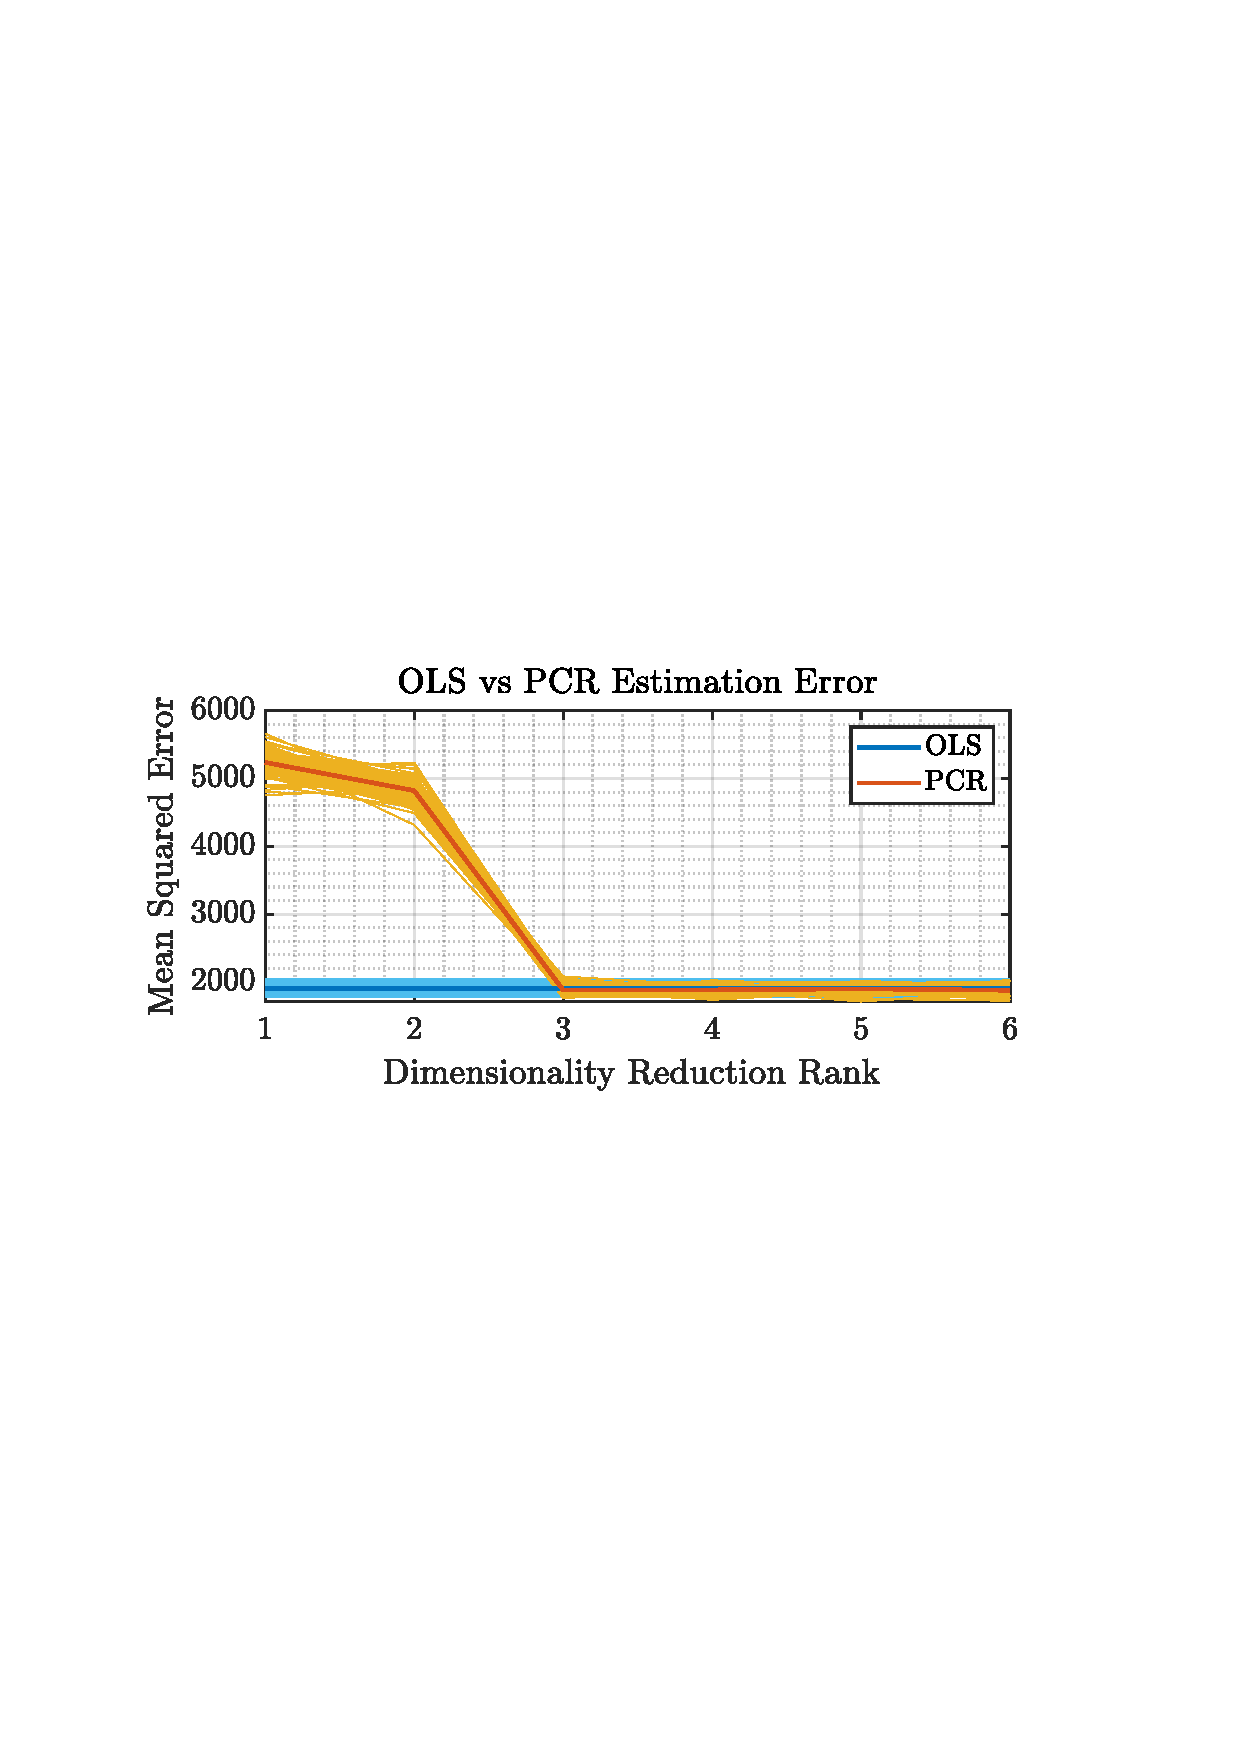
\includegraphics[trim={2.2cm 11.2cm 3.15cm  11.2cm}, clip, width=\textwidth]{../MATLAB/figures/q1_6d_fig01.pdf} 
	 		\captionsetup{justification=centering}
	 		\captionof{figure}{Mean Square Error over several Realisations}
	 		\label{fig: 1-6d}
	 	\end{minipage}%
 
\pagebreak
\section{Adaptive Signal Processing} \label{sec: 2-ASP}
	\subsection{The Least Mean Square (LMS) Algorithm} \label{sec: 2-1-LMS}
		\subsubsection{Example Correlation Matrix}
			A general AR(2) process $x(n)$ with parameters $a_{1}, a_{2}$ satisfies the difference equation:
			
			\begin{equation}
			x(n) = a_{1} x(n - 1) + a_{2} x(n - 2) + \eta(n)
			\label{eq: 2-1a-ar_2}
			\end{equation}
			
			where $\eta(n) \sim \mathcal{N}(0, \sigma_{\eta}^{2})$. The Least Mean Square (LMS) algorithm is used to approximate
			the autoregressive parameters $a_{1}, a_{2}$ from data, treating $\mathbf{x}(n) = [x(n-1), x(n-2)]^{T}$ and
			$y(n) = x(n)$ as the input (features) vector and the output (target), respectively.
			
			The correlation matrix $\mathbf{R}_{xx}$ of the input vector $\mathbf{x}(n)$ is given by:
			
			\begin{equation}
			\mathbf{R}_{xx} = \E[\mathbf{x}(n) \mathbf{x}^{T}(n)] = \E
			\begin{bmatrix}
			x(n-1) x(n-1) & x(n-1) x(n-2) \\
			x(n-1) x(n-2) & x(n-2) x(n-2)
			\end{bmatrix} =
			\begin{bmatrix}
			r_{xx}(0) & r_{xx}(1) \\
			r_{xx}(1) & r_{xx}(0)
			\end{bmatrix}
			\label{eq: 2-1a-cov_ar_2}
			\end{equation}
			
			where $r_{xx}(k)$ the autocorrelation function (ACF) of $x(n)$. To obtain the ACF of the AR(2) process, multiply equation (\ref{eq: 2-1a-ar_2}) by $x(n-k)$ and take expectations:
			
			\begin{align}
			r_{xx}(k) = \E[ x(n) x(n-k) ]   &= \E \bigg[ a_{1} x(n - 1) x(n-k) + a_{2} x(n - 2) x(n-k) + \eta(n) x(n-k) \bigg] \nonumber\\
			r_{xx}(k) = \E[ x(n) x(n-k) ]   &= a_{1} \E \big[ x(n - 1) x(n-k) \big] + a_{2} \E \big[ x(n - 2) x(n-k) \big] + \E \big[ \eta(n) x(n-k) \big]
			\end{align}
			
			Notice that $\E [\eta(n) x(n-k)]$ vanishes when $k > 0$, then:
			
			\begin{align}
			r_{xx}(0)   &= a_{1} r_{xx}(1) + a_{2} r_{xx}(2) + \sigma_{\eta}^{2} \\
			r_{xx}(k)   &= a_{1} r_{xx}(k-1) + a_{2} r_{xx}(k-2), k > 0
			\label{eq: 2-1a-acf_ar_2}
			\end{align}
			
			Note that ACF is an even function or equivalently $r_{xx}(-k) = r_{xx}(k), \forall k \in \setInteger$, thus using the true process parameters $a_{1} = 0.1$, $a_{2} = 0.8$
			and $\sigma_{\eta}^{2} = 0.25$, we obtain the three simultaneous equations with three unknowns:
			
			\begin{align}
			r_{xx}(0)   &= a_{1} r_{xx}(1) + a_{2} r_{xx}(2) + \sigma_{\eta}^{2} \\
			r_{xx}(1)   &= a_{1} r_{xx}(0) + a_{2} r_{xx}(-1) = a_{1} r_{xx}(0) + a_{2} r_{xx}(1) \\
			r_{xx}(2)   &= a_{1} r_{xx}(1) + a_{2} r_{xx}(0)
			\end{align}
			
			with the unique solution $r_{xx}(k) = [\frac{25}{27}, \frac{25}{54}, \frac{85}{108}]$ for $k=1, 2, 3$.
			
			Hence by substitution in equation (\ref{eq: 2-1a-cov_ar_2}) we obtain the  correlation matrix of the input vector $\mathbf{x}(n)$:
			
			\begin{equation}
			\mathbf{R}_{xx} = 
			\frac{25}{54}
			\begin{bmatrix}
			2 & 1 \\
			1 & 2
			\end{bmatrix}
			\label{eq: 2-1a-cov_ar_2_result}
			\end{equation}
			
			Convergence of the LMS algorithm depends on the step size $\mu$, which should satisfy:
			
			\begin{equation}
			0 < \mu < \frac{2}{\lambda_{max}}
			\label{eq: 2-1a-cond:mu_max}
			\end{equation}
			
			where $\lambda_{max}$ the largest eigenvalue of the correlation matrix $\mathbf{R}_{xx}$. Performing the eigendecomposition of $\mathbf{R}_{xx}$, we obtain
			$\lambda_{1} = 0.4630$ and $\lambda_{2} = \lambda_{max} = 1.3889$ and as a result, convergence to the Wiener optimal solution is guaranteed for:
			
			\begin{equation}
			0 < \mu < 1.44
			\label{eq: 2-1a-cond:mu_max_val}
			\end{equation}
		\subsubsection{Example Learning Curve for an AR(2) Process}
		
			\begin{figure}[H]
				\centering
				\begin{subfigure}{0.49\textwidth}
					\centering
					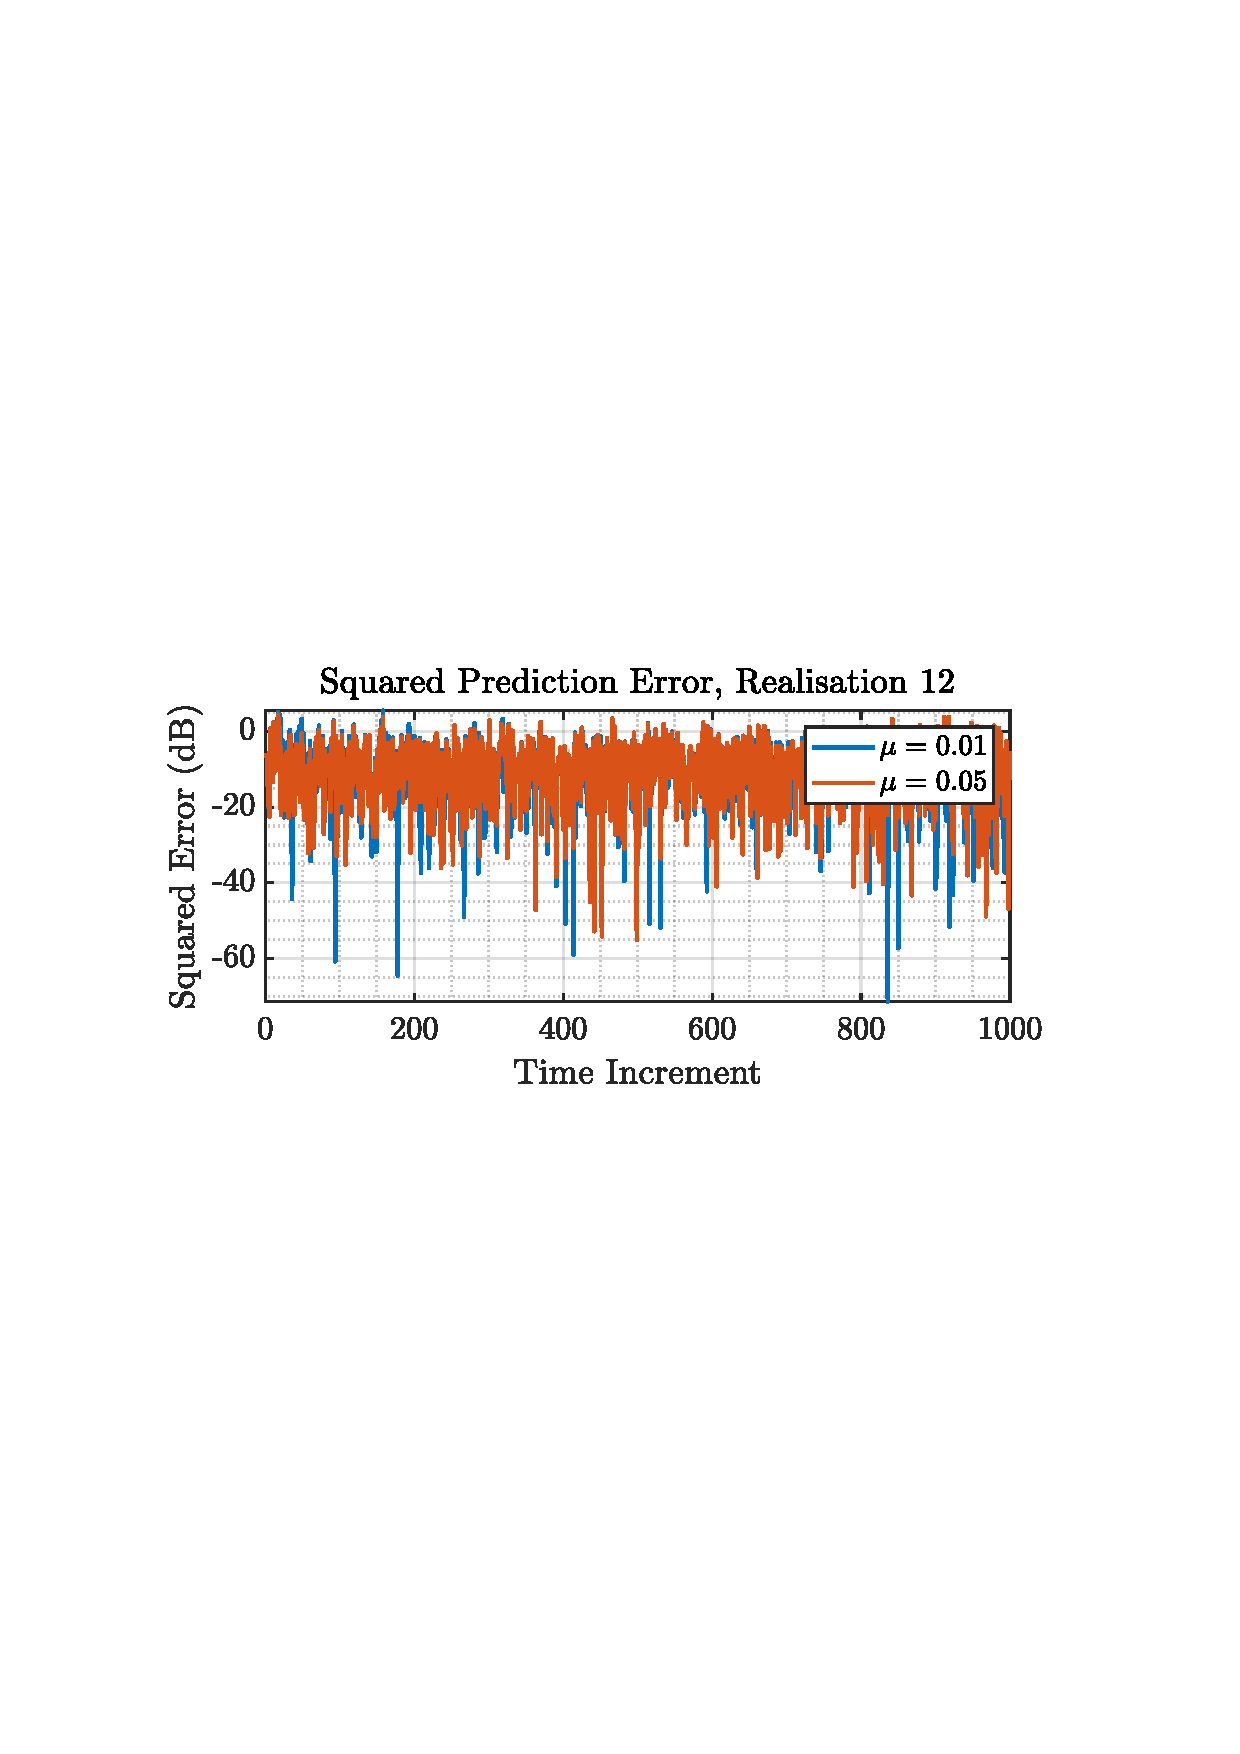
\includegraphics[trim={2.2cm 11.2cm 3.15cm  11.2cm}, clip, width=\textwidth]{../MATLAB/figures/q2_1b_fig01.pdf} 
					\captionsetup{justification=centering}
					\caption{Square Prediction Error, Single Realisation}
				\end{subfigure}
				%		~ % forces onto the same row
				\begin{subfigure}{0.49\textwidth}
					\centering
					\includegraphics[trim={2.2cm 11.2cm 3.15cm  11.2cm}, clip, width=\textwidth]{../MATLAB/figures/q2_1b_fig03.pdf} 
					\captionsetup{justification=centering}
					\caption{Log of Mean of the Squared Prediction Error}
				\end{subfigure}
				\captionsetup{justification=centering}
				\caption{$\mu$'s effect on the Squared Prediction Error and the Influence of the Log operator}
				\label{fig: 2-1b}
			\end{figure}
		
		As can be seen in Figure \ref{fig: 2-1b}, the log operator exponentially emphasises the small trends in the error signal. It is now easier to see the influence of the higher $\mu$ on reaching steady state, where we can see that larger values converge faster.
		
		\subsubsection{Misadjustment}
			
			The theoretical Misadjustment, $\mathcal{M}_{LMS}$, of the LMS algorithm is obtained by the approximation formula:
			
			\begin{equation}
			\mathcal{M}_{LMS} \approx \frac{\mu}{2} Tr\big\{ \mathbf{R}_{xx} \big\} = \frac{\mu}{2} 1.8519
			\end{equation}
			
			where $\mathbf{R}_{xx}$ from (\ref{eq: 2-1a-cov_ar_2_result}) is used.
			
			According to figure \ref{fig: 2-1b} the squared prediction error plateaus for both $\mu$ values after $t > 200$. To guarantee that a steady-state has been reached, we time average the squared prediction error for $t_{0} > 400$, in order to obtain a Mean Squared Error (MSE) estimate. The empirical misadjustment, $\mathcal{M}_{emp}$,
			is then obtained using the formula:
			
			\begin{equation}
			\mathcal{M}_{emp} = \frac{\mathtt{EMSE}}{\sigma_{\eta}^{2}} = \frac{\mathtt{MSE}}{\sigma_{\eta}^{2}} -1
			\end{equation}
			
			Table \ref{tab: 2-1c} summarises the empirical, theoretical and practical misadjustments of the simple LMS algorithm for the $x(n)$ process.
						
			\begin{table}[H]
				\centering
				\begin{tabular}{|c|c|c||c|}
					\hline
					\textbf{$\mu$} & \textbf{$\mathcal{M}_{emp}$} & Theoretical \textbf{$\mathcal{M}_{LMS}$} & Practical \textbf{$\mathcal{M}_{LMS}$} \\
					\hline
					0.01 & $0.0093$ & $0.0077$ & $0.0182 \pm 0.05619$ \\
					\hline
					0.005 & $0.0463$ & $0.0491$ & $0.0593 \pm 0.06409$ \\
					\hline
				\end{tabular}
				\captionsetup{justification=centering}
				\caption{Theoretical and LMS Estimated Misadjustments}
				\label{tab: 2-1c}
			\end{table}
		
			\begin{minipage}[b]{0.49\textwidth}
				Misadjustment for larger $\mu$ values appears to be larger, corresponding to what is observed in Figure \ref{fig: 2-1b} and \ref{fig: 2-1d}, where larger MSE is contributing to this difference. It is clear that the standard deviations of misadjustment are very large in the practical data.
			\end{minipage}% 
			\begin{minipage}{0.04\textwidth}
				\hspace*{0.04\textwidth}
			\end{minipage}% 
			\begin{minipage}[t]{0.49\textwidth}
				\centering
				\includegraphics[trim={2.2cm 11.2cm 3.15cm  11.2cm}, clip, width=\textwidth]{../MATLAB/figures/q2_1cd_fig01.pdf} 
				\captionsetup{justification=centering}
				\captionof{figure}{Estimated Misadjustment, varying with realisation. $\mathcal{M}_{LMS}$ is additionally plotted for reference. }
				\label{fig: 2-1c}			
			\end{minipage}%

		\subsubsection{Steady State Estimation} 
			\begin{figure}[H]
				\centering
				\begin{subfigure}{0.49\textwidth}
					\centering
					\includegraphics[trim={2.2cm 11.2cm 3.00cm  11.2cm}, clip, width=\textwidth]{../MATLAB/figures/q2_1cd_fig02.pdf} 
					\captionsetup{justification=centering}
				\end{subfigure}
				%		~ % forces onto the same row
				\begin{subfigure}{0.49\textwidth}
					\centering
					\includegraphics[trim={2.2cm 11.2cm 3.00cm  11.2cm}, clip, width
					=\textwidth]{../MATLAB/figures/q2_1cd_fig03.pdf} 
					\captionsetup{justification=centering}
				\end{subfigure}
				\captionsetup{justification=centering}
				\caption{$\mu$'s effect on weight stabilisation}
				\label{fig: 2-1d}
			\end{figure}
		The simulation shown in Figure \ref{fig: 2-1d}, shows that convergence to a steady state is faster with larger $\mu$ values, 200 ($\mu=0.05$) vs 900 ($\mu=0.01$), however, we observe that the converged value is less accurate and more noisy, as can be clearly seen for $\hat{a}_1$.
		\subsubsection{Leaky LMS Derivation}
			Let the objective function $\mathcal{J}_{2}$, such that:
			
			\begin{equation}
			\mathcal{J}_{2}(n) = \frac{1}{2} \bigg( e^{2}(n) + \gamma \| \vw(n) \|_{2}^{2} \bigg)
			\label{eq: 2-1e-J_2}
			\end{equation}
			
			Expressing the error term, $e(n)$, in terms of the input vector $\mathbf{x}_{n}$ and the target value $y_{n}$:
			
			\begin{align}
			\mathcal{J}_{2}(n)  &= \frac{1}{2} \bigg( \| y(n) - \vw(n)^{T} \mathbf{x}(n) \|_{2}^{2} + \gamma \| \vw(n) \|_{2}^{2} \bigg) \\
			\mathcal{J}_{2}(n)  &= \frac{1}{2} \bigg( \big( y(n) - \vw(n)^{T} \mathbf{x}(n))^{T} (y(n) - \vw(n)^{T} \mathbf{x}(n) \big) + \gamma \vw(n)^{T} \vw(n) \bigg)
			\end{align}
			
			Calculating the gradient of the objective function, $\nabla_{\vw} \mathcal{J}_{2}$, with respect to the weights $\vw$:
			
			\begin{align}
			\nabla_{\vw} \mathcal{J}_{2}(n) &= - ( y(n) - \vw(n)^{T} \mathbf{x}(n) ) \mathbf{x}(n) + \gamma \vw(n) \\
			\nabla_{\vw} \mathcal{J}_{2}(n) &= - e(n) \mathbf{x}(n) + \gamma \vw(n)
			\end{align}
			
			Applying the gradient descent update to weights $\vw$ to minimise the objective function $\mathcal{J}_{2}$:
			
			\begin{align}
			\vw(n + 1)  &= \vw(n) - \mu \nabla_{\vw} \mathcal{J}_{2}(n) \\
			\vw(n + 1)  &= \vw(n) - \mu \big( - e(n) \mathbf{x}(n) + \gamma \vw(n) \big) \\
			\vw(n + 1)  &= (1 - \mu \gamma) \vw(n) + \mu e(n) \mathbf{x}(n)
			\label{eq: 2-1e-leaky_lms}
			\end{align}
			
			Hence we proved that the Leaky LMS algorithm following the update rule in (\ref{eq: 2-1e-leaky_lms}) is equivalent to the minimisation of the objective function $\mathcal{J}_{2}$
			defined in (\ref{eq: 2-1e-J_2}).
		\subsubsection{Example Leaky LMS for an AR(2) Process}  
		
			\begin{figure}[H]
				\centering
				\begin{subfigure}{0.49\textwidth}
					\centering
					\includegraphics[trim={2.2cm 11.2cm 3.00cm  11.2cm}, clip, width=\textwidth]{../MATLAB/figures/q2_1f_fig01.pdf} 
					\captionsetup{justification=centering}
				\end{subfigure}
				%		~ % forces onto the same row
				\begin{subfigure}{0.49\textwidth}
					\centering
					\includegraphics[trim={2.2cm 11.2cm 3.00cm  11.2cm}, clip, width=\textwidth]{../MATLAB/figures/q2_1f_fig02.pdf} 
					\captionsetup{justification=centering}
				\end{subfigure}
			
				\begin{subfigure}{0.49\textwidth}
					\centering
					\includegraphics[trim={2.2cm 11.2cm 3.00cm  11.2cm}, clip, width=\textwidth]{../MATLAB/figures/q2_1f_fig04.pdf} 
					\captionsetup{justification=centering}
				\end{subfigure}
				%		~ % forces onto the same row
				\begin{subfigure}{0.49\textwidth}
					\centering
					\includegraphics[trim={2.2cm 11.2cm 3.00cm  11.2cm}, clip, width=\textwidth]{../MATLAB/figures/q2_1f_fig05.pdf} 
					\captionsetup{justification=centering}
				\end{subfigure}
			
				\begin{subfigure}{0.49\textwidth}
					\centering
					\includegraphics[trim={2.2cm 11.2cm 3.00cm  11.2cm}, clip, width=\textwidth]{../MATLAB/figures/q2_1f_fig07.pdf} 
					\captionsetup{justification=centering}
				\end{subfigure}
				%		~ % forces onto the same row
				\begin{subfigure}{0.49\textwidth}
					\centering
					\includegraphics[trim={2.2cm 11.2cm 3.00cm  11.2cm}, clip, width=\textwidth]{../MATLAB/figures/q2_1f_fig08.pdf} 
					\captionsetup{justification=centering}
				\end{subfigure}
				\captionsetup{justification=centering}
				\caption{$\gamma$'s leakage, forgetful, effect on weight stabilisation}
				\label{fig: 2-1f}
			\end{figure}
		
		The leaky LMS implements the term $\gamma$, which we can interpret as a forgetfulness term, where the LMS filter forgets the previous weight's significance. This means that the filter reaches a steady state faster, which can be observed in Figure \ref{fig: 2-1f}, where we see convergence is 400 steps instead of 900 when using $\gamma=0.5$. \\
		Importantly, the accuracy is greatly compromised, the magnitude of the error is directly proportional to the $\gamma$ used.
		 
	\subsection{Adaptive Step Sizes} \label{sec: 2-2-adaptive-step}
		\subsubsection{Gradient Adaptive Step Sizes (GASS) Comparisons for a MA(1) System} 
			\begin{figure}[H]
				\centering
				\begin{subfigure}{0.49\textwidth}
					\centering
					\includegraphics[trim={2.2cm 11.2cm 3.15cm  11.2cm}, clip, width=\textwidth]{../MATLAB/figures/q2_2a_fig03.pdf} 
					\captionsetup{justification=centering}
				\end{subfigure}
				%		~ % forces onto the same row
				\begin{subfigure}{0.49\textwidth}
					\centering
					\includegraphics[trim={2.2cm 11.2cm 3.15cm  11.2cm}, clip, width=\textwidth]{../MATLAB/figures/q2_2a_fig04.pdf} 
					\captionsetup{justification=centering}
				\end{subfigure}
				\captionsetup{justification=centering}
				\caption{Weight Error and Prediction Error for various GASS algorithms}
				\label{fig: 2-2a}
			\end{figure}
		Varying our $\mu$ term would allow us to learn faster, by taking larger steps of change in our weights, for example when the error is large. What we observe in the gradients in the (log emphasised) mean square error plot, Figure \ref{fig: 2-2a}, is the effective learning rate for these algorithms. Additionally we can see the influence of changing the algorithm's starting learning rate, and its effect on convergence. It is clear that the Beneviste algorithm has the faster convergence, but when looking at the effect of increasing $\mu$ we observe the improvement of learning rate (increase of gradient magnitude) in descending order is: LMS, Matthews \& Xie then Ang \& Farhang.\\
		In the highly dynamic applications where such filters would be needed, we can imagine that the learning rate can influence the output properties when compared to the desired output. For example, if the learning rate was less than or equal to the applications fluctuation rate we would observe a low pass filter effect, as the predicted output would not necessarily reach the actual output in the time between fluctuations.
		
		\subsubsection{NLMS Update Equation Equivalence}
			Starting from the update equation based on the \textit{a posteriori error} $e_{p}(n) = d(n) - \mathbf{x}(n)^{T} \vw(n + 1)$:
			
			\begin{equation}
			\vw(n + 1) = \vw(n) + \mu e_{p}(n) \mathbf{x}(n)
			\label{eq:nlms_a_error}
			\end{equation}
			
			Multiply both sides with $-\mathbf{x}(n)^{T}$ and add $d(n)$ to construct $e_{p}(n)$ on the LHS:
			
			\begin{equation}
			d(n) - \mathbf{x}(n)^{T} \vw(n + 1) = d(n) - \mathbf{x}(n)^{T} \vw(n) - \mathbf{x}(n)^{T} \mu e_{p}(n) \mathbf{x}(n)
			\end{equation}
			
			Note that the LHS term is the a posteriori error, $e_{p}(n)$, while the first RHS term the a priori error, $e(n)$:
			
			\begin{align}
			e_{p}(n)    &= e(n) - \mu e_{p}(n) \| \mathbf{x}(n) \|^{2} \\
			e_{p}(n)    &= e(n) \frac{1}{1 + \mu \| \mathbf{x}(n) \|^{2}}
			% &= e(n) \bigg[ \frac{1 + \mu \| \mathbf{x}(n) \|^{2} - \mu \| \mathbf{x}(n) \|^{2} }{1 + \mu \| \mathbf{x}(n) \|^{2}} \bigg] \\
			% &= e(n) \bigg[ 1 - \mu \frac{\| \mathbf{x}(n) \|^{2}}{1 + \mu \| \mathbf{x}(n) \|^{2}} \bigg]
			\label{eq:aa_errors}
			\end{align}
			
			Substituting (\ref{eq:aa_errors}) in update equation (\ref{eq:nlms_a_error}):
			
			\begin{align}
			\vw(n + 1)  &= \vw(n) + \mu \frac{1}{1 + \mu \| \mathbf{x}(n) \|^{2}} e(n) \mathbf{x}(n) \\
			\vw(n + 1)  &= \vw(n) + \frac{1}{\frac{1}{\mu} + \| \mathbf{x}(n) \|^{2}} e(n) \mathbf{x}(n) \\
			\vw(n + 1)  &= \vw(n) + \frac{\beta}{\epsilon + \| \mathbf{x}(n) \|^{2}} e(n) \mathbf{x}(n) \label{eq:nlms}
			\end{align}
			
			where for $\beta = 1$ and $\epsilon = \frac{1}{\mu}$ we showed that the NLMS update (\ref{eq:nlms}) is equivalent to the update equation based on the \textit{a posteriori error},
			given by (\ref{eq:nlms_a_error}).
		
		 
		\subsubsection{Generalised Normalised Gradient Descent (GNGD) Example for a MA(1) System} 
		
			\begin{figure}[H]
				\centering
				\begin{subfigure}{0.49\textwidth}
					\centering
					\includegraphics[trim={2.2cm 11.2cm 3.15cm  11.2cm}, clip, width=\textwidth]{../MATLAB/figures/q2_2c_fig03.pdf} 
					\captionsetup{justification=centering}
				\end{subfigure}
				%		~ % forces onto the same row
				\begin{subfigure}{0.49\textwidth}
					\centering
					\includegraphics[trim={2.2cm 11.2cm 3.15cm  11.2cm}, clip, width=\textwidth]{../MATLAB/figures/q2_2c_fig04.pdf} 
					\captionsetup{justification=centering}
				\end{subfigure}
				\captionsetup{justification=centering}
				\caption{Weight Error and Prediction Error comparing the GNGD NLMS to the Benveniste GASS Algorithm}
				\label{fig: 2-2c}
			\end{figure}
		
			As we explored earlier the LMS algorithm's convergence time is closely tied to the value of $\mu$, showing the greatest change for the $\times10$ increase of $\mu$. Figure \ref{fig: 2-2c}, shows that we can surpass the rate of convergence of the Benveniste algorithm when using the NLMS algorithm. The NLMS algorithm allows us to choose large values of $\mu$, that would traditionally cause the output of the LMS to be unstable, due to its GNGD normalisation approach.
			
	\subsection{Adaptive Noise Cancellation} \label{sec: 2-3-ANC}
		Let the pure sine wave $x(n)$, the noisy signal $s(n)$, the noise term $\eta(n)$ and the ALE filter output $\hat{x}(n; \Delta)$, parametrised by the delay parameter $\Delta$.
		Then the Mean Squared Error (MSE) is given by:
		
		\begin{align}
		\mathtt{MSE} =
		\E \bigg[ \big( s(n) - \hat{x}(n; \Delta) \big)^{2} \bigg]  &=  \E \bigg[ \big( x(n) + \eta(n) - \hat{x}(n; \Delta) \big)^{2} \bigg] \\
		&=  \E \bigg[ \big( \eta(n) + (x(n) - \hat{x}(n; \Delta)) \big)^{2} \bigg] \\
		&=  \E \bigg[ \eta^{2}(n) \bigg] +
		\E \bigg[ \big( x(n) - \hat{x}(n; \Delta) \big)^{2} \bigg] +
		2\E \bigg[ \eta(n) \big(x(n) - \hat{x}(n; \Delta) \big) \bigg]
		\label{eq:ale_mse}
		\end{align}
		
		The first term, noise power $\E [ \eta^{2}(n) ]$, is independent of $\Delta$, while the second term, Mean Squared Prediction Error $\E [ (x(n) - \hat{x}(n; \Delta))^{2} ]$ is not
		a function of noise $\eta(n)$. Hence, the last term only involves both the delay $\Delta$ (through $\hat{x}(n)$) and the noise term, so we will minimise it:
		
		\begin{equation}
		\underset{\Delta \in \setNatural}{min}\ \E \bigg[ \eta(n) \big(x(n) - \hat{x}(n; \Delta) \big) \bigg]
		\end{equation}
		
		Using the fact that $x(n)$ and $\eta(n)$ are uncorrelated the term $\E [ \eta(n) x(n) ]$ vanished:
		
		\begin{align}
		\underset{\Delta \in \setNatural}{min}\ \E \bigg[ \eta(n) \hat{x}(n; \Delta) \bigg] &\rightarrow
		\underset{\Delta \in \setNatural}{min}\ \E \bigg[ \big( u(n) + 0.5u(n-2) \big) \vw^{T} \vu(n; \Delta) \bigg] \\
		&\rightarrow
		\underset{\Delta \in \setNatural}{min}\ \E \bigg[ \big( u(n) + 0.5u(n-2) \big) \sum_{i=0}^{M-1} w_{i} s(n - \Delta - i) \bigg] \\
		&\rightarrow
		\underset{\Delta \in \setNatural}{min}\ \E \bigg[ \big( u(n) + 0.5u(n-2) \big) \sum_{i=0}^{M-1} w_{i} \big( x(n - \Delta - i) + \eta(n - \Delta - i) \big) \bigg] \\
		&\rightarrow
		\underset{\Delta \in \setNatural}{min}\ \E \bigg[ \big( u(n) + 0.5u(n-2) \big) \sum_{i=0}^{M-1} w_{i} \big( \eta(n - \Delta - i) \big) \bigg] \\
		&\rightarrow
		\underset{\Delta \in \setNatural}{min}\ \E \bigg[ \big( u(n) + 0.5u(n-2) \big) \sum_{i=0}^{M-1} w_{i} \big( u(n - \Delta - i) + 0.5 u(n - 2 - \Delta - i) \big) \bigg]
		\label{con:delta} \\
		&\rightarrow
		0, \quad \Delta > 2
		\end{align}
		
		Since $u(n)$ is identically and \textbf{independently} distributed white noise:
		
		\begin{equation}
		\E \bigg[ u(n) u(n - j) \bigg] = 0, \quad \forall j \neq 0
		\end{equation}
		
		therefore the expectation in (\ref{con:delta}) is zero and thus minimised for $\Delta > 2$, since the terms are non time-overlapping.
		This is an expected result, since the colored noise signal $\eta(n)$ is a second order MA process.
		
		The theoretical optimal delay range, $\Delta > 2$ is also verified empirically. \\
		The MPSE as a function of $\Delta$ is also plotted in Figure \ref{fig: 2-3a}, verifying the improved performance $\Delta > 2$.
		
		\subsubsection{Adaptive Line Enhancer (ALE) Delay Investigation}
		\begin{minipage}[b]{0.49\textwidth}
%			\subsubsection{Adaptive Line Enhancer (ALE) Delay Investigation}
				Figure \ref{fig: 2-3a} shows the influence of ALE Delay on a range of model orders. We can see the minimum MPSE for Delay of 5 for Model Order 5. As we increase the delay we see a linear increase in log emphasised MPSE, letting us know that the samples that are more than 5 time points away are increasingly uncorrelated to the current prediction, as expected for this second order moving average process.
%			\subsubsection{Adaptive Line Enhancer (ALE) Filter Order Investigation}
%				Figure \ref{fig: 2-3b} shows the influence of ALE Model Order for a given delay. This hyper parameter sweep is informative in understanding how many samples are needed to appropriately model the noise system, in this case we see that orders of 3 and 5 give us minimum MPSE. As we start to overfit with increasing model orders we get increasingly worse predictions.
		\end{minipage}% 
		\begin{minipage}{0.04\textwidth}
			\hspace*{0.04\textwidth}
		\end{minipage}% 
		\begin{minipage}[t]{0.49\textwidth}
			\centering
			\includegraphics[trim={2.2cm 11.2cm 3.15cm  11.2cm}, clip, width=\textwidth]{../MATLAB/figures/q2_3b_fig02.pdf} 
			\captionsetup{justification=centering}
			\captionof{figure}{ALE Delay \& Order Sweep}
			\label{fig: 2-3a}
%			\vspace*{10px}
%			\centering
%			\includegraphics[trim={2.2cm 11.2cm 3.15cm  11.2cm}, clip, width=\textwidth]{../MATLAB/figures/q2_3b_fig03.pdf} 
%			\captionsetup{justification=centering}
%			\captionof{figure}{ALE Order Sweep}
%			\label{fig: 2-3b}
		\end{minipage}%
	
	\subsubsection{Adaptive Line Enhancer (ALE) Filter Order Investigation}
		\begin{minipage}[b]{0.49\textwidth}
%			\subsubsection{Adaptive Line Enhancer (ALE) Delay Investigation}
			Figure \ref{fig: 2-3b} shows the influence of ALE Model Order for a given delay. This hyper parameter sweep is informative in understanding how many samples are needed to appropriately model the noise system, in this case we see that orders of 3 and 5 give us minimum MPSE. As we start to overfit with increasing model orders we get increasingly worse predictions.
		\end{minipage}% 
		\begin{minipage}{0.04\textwidth}
			\hspace*{0.04\textwidth}
		\end{minipage}% 
		\begin{minipage}[t]{0.49\textwidth}
			\centering
			\includegraphics[trim={2.2cm 11.2cm 3.15cm  11.2cm}, clip, width=\textwidth]{../MATLAB/figures/q2_3b_fig03.pdf} 
			\captionsetup{justification=centering}
			\captionof{figure}{ALE Order Sweep}
			\label{fig: 2-3b}
		\end{minipage}%
		
		
		\subsubsection{Adaptive Noise Cancellation (ANC) Comparison}
			\begin{figure}[H]
				\centering
				\begin{subfigure}{0.49\textwidth}
					\centering
					\includegraphics[trim={2.2cm 11.2cm 3.00cm  11.2cm}, clip, width=\textwidth]{../MATLAB/figures/q2_3c_fig01.pdf} 
					\captionsetup{justification=centering}
				\end{subfigure}
				%		~ % forces onto the same row
				\begin{subfigure}{0.49\textwidth}
					\centering
					\includegraphics[trim={2.2cm 11.2cm 3.00cm  11.2cm}, clip, width=\textwidth]{../MATLAB/figures/q2_3c_fig02.pdf} 
					\captionsetup{justification=centering}
				\end{subfigure}
				\captionsetup{justification=centering}
				\caption{ALE and ANC compared, MSPE was calculated from time index 600+}
				\label{fig: 2-3c}
			\end{figure}
		
			To compare the ANC and ALE algorithms we fixed the Model Order to $M=6$ and set the ALE Delay to $\Delta=3$. This ALE Delay is one of the optimums as shown in Figure \ref{fig: 2-3a}. What we observe in Figure \ref{fig: 2-3c}, is the 15 times better MPSE performance of the ANC algorithm.\\
			When looking at the ensemble of predicted traces for both algorithms we see that the ANC stabilisation time is longer than that of ALE, but the stabilised prediction is much closer to the true signal. The mean trace shows us that there is both an amplitude error and phase error for the ALE predictor, which is not seen in the ALE predictor.
		
		\subsubsection{Adaptive Noise Cancellation (ANC) on real EEG Data}
			\begin{figure}[H]
				\centering
				\begin{subfigure}{0.49\textwidth}
					\centering
					\includegraphics[trim={2.2cm 11.2cm 2.70cm  11.2cm}, clip, width=\textwidth]{../MATLAB/figures/q2_3d_fig01.pdf} 
					\captionsetup{justification=centering}
				\end{subfigure}
				%		~ % forces onto the same row
				\begin{subfigure}{0.49\textwidth}
					\centering
					\includegraphics[trim={2.8cm 11.2cm 3.00cm  11.2cm}, clip, width=\textwidth]{../MATLAB/figures/q2_3d_fig06.pdf} 
					\captionsetup{justification=centering}
				\end{subfigure}
				
				\captionsetup{justification=centering}
				\caption{ Original Spectrogram \& investigating hyperparameters. \\
						  50Hz was defined with a $\pm$2Hz window. }
				\label{fig: 2-3d-orig+paramSweep}
			\end{figure}
		
			As we can see above in Figure \ref{fig: 2-3d-orig+paramSweep}, a hyper parameter heatmap highlights the RMSE tradeoffs we can expect for varying model order, $M$, and learning rate, $\mu$, with this EEG dataset. Using this knowledge we selected $M=10,\mu=0.01$ as the best parameters. 
			
			\begin{figure}[H]
				\centering
				\begin{subfigure}{0.49\textwidth}
					\centering
					\includegraphics[trim={2.2cm 11.2cm 3.15cm  11.2cm}, clip, width=\textwidth]{../MATLAB/figures/q2_3d_fig02.pdf} 
					\captionsetup{justification=centering}
				\end{subfigure}
				%		~ % forces onto the same row
				\begin{subfigure}{0.49\textwidth}
					\centering
					\includegraphics[trim={2.2cm 11.2cm 2.70cm  11.2cm}, clip, width=\textwidth]{../MATLAB/figures/q2_3d_fig03.pdf} 
					\captionsetup{justification=centering}
				\end{subfigure}
				
				\begin{subfigure}{0.49\textwidth}
					\centering
					\includegraphics[trim={2.2cm 11.2cm 3.15cm  11.2cm}, clip, width=\textwidth]{../MATLAB/figures/q2_3d_fig04.pdf} 
					\captionsetup{justification=centering}
				\end{subfigure}
				%		~ % forces onto the same row
				\begin{subfigure}{0.49\textwidth}
					\centering
					\includegraphics[trim={2.2cm 11.2cm 2.70cm  11.2cm}, clip, width=\textwidth]{../MATLAB/figures/q2_3d_fig05.pdf} 
					\captionsetup{justification=centering}
				\end{subfigure}
				\captionsetup{justification=centering}
				\caption{$\mu$'s effect on noise cancellation}
				\label{fig: 2-3d}
			\end{figure}
		
			In Figure \ref{fig: 2-3d}, we can see that using the selected parameters neatly seals off the 50Hz noise. When we investigate the influence of the greater learning rate, we see great attenuation around the 50Hz band spreading by 25Hz to the surrounding frequencies. Additionally, we can see an amplification in the harmonic of the 50Hz noise, at 100Hz. \\
			
			It is important to highlight the significance of the external noise fed into the ANC algorithm, testing showed that increasing the noisiness of the provided input noise signal drastically reduced ANC performance, outputs were unstable and rapidly approached infinity, becoming more prominent for larger $\mu$. In the example in Figure \ref{fig: 2-3d} a 50Hz signal was generated with noise power $\sigma_n^{ 2}=0.1$.\\
			 In technology where this algorithm would be useful, such as noise cancelling headphones, we would ensure that the noise external microphones pick up have a known linear relationship to what is heard inside the headphones. If this relationship is not approximately linear we can imagine that the noise cancellation effect would be less pronounced, unless other preprocessing is used before being fed into the ANC algorithm.
	
\pagebreak
\section{Widely Linear Filtering and Adaptive Spectrum Estimation} \label{sec: 3-WLASE}
	\subsection{Complex LMS and Widely Linear Modelling} \label{sec: 3-1-CLMS-ACLMS}
		\subsubsection{Widely Linear Moving Average (WLMA) Process using Complex LMS (CLMS) \& Augmented CLMS (ACLMS)}
			\begin{figure}[H]
				\centering
				\begin{subfigure}{0.49\textwidth}
					\centering
					\includegraphics[trim={2.2cm 11.2cm 3.00cm  11.2cm}, clip, width=\textwidth]{../MATLAB/figures/q3_1a_fig01.pdf} 
					\captionsetup{justification=centering}
				\end{subfigure}
				%		~ % forces onto the same row
				\begin{subfigure}{0.49\textwidth}
					\centering
					\includegraphics[trim={2.2cm 11.2cm 3.00cm  11.2cm}, clip, width=\textwidth]{../MATLAB/figures/q3_1a_fig02.pdf} 
					\captionsetup{justification=centering}
				\end{subfigure}
				
				\captionsetup{justification=centering}
				\caption{Data Circularity's and the suitability of CLMS \& ACLMS to model a WLMA(1) }
				\label{fig: 3-1a}
			\end{figure}
			
			Figure \ref{fig: 3-1a}, shows the difference in circularity of white gaussian noise and the first order widely linear moving average process. Additionally, we can see the CLMS learning curve struggle to model the non-circular WLMA(1) process, converging to an MSPE $>0$dB.
			
		\subsubsection{CLMS and ACLMS Suitability with real (wind) data}
			\begin{figure}[H]
				\centering
				\begin{subfigure}{0.49\textwidth}
					\centering
					\includegraphics[trim={2.2cm 11.2cm 3.15cm  11.2cm}, clip, width=\textwidth]{../MATLAB/figures/q3_1b_fig04.pdf} 
				\end{subfigure}
				\begin{subfigure}{0.49\textwidth}
					\centering
					\includegraphics[trim={2.2cm 11.2cm 3.15cm  11.2cm}, clip, width=\textwidth]{../MATLAB/figures/q3_1b_fig05.pdf} 
				\end{subfigure}
				%		~ % forces onto the same row
				\begin{subfigure}{0.49\textwidth}
					\centering
					\includegraphics[trim={2.2cm 11.2cm 3.15cm  11.2cm}, clip, width=\textwidth]{../MATLAB/figures/q3_1b_fig06.pdf} 
				\end{subfigure}
				%		~ % forces onto the same row
				\begin{subfigure}{0.49\textwidth}
					\centering
					\includegraphics[trim={2.2cm 11.2cm 3.15cm  11.2cm}, clip, width=\textwidth]{../MATLAB/figures/q3_1b_fig07.pdf} 
				\end{subfigure}			
				\captionsetup{justification=centering}
				\captionof{figure}{Wind Regime Circularity and CLMS \& ACLMS estimates \\
					Low, Medium and High Regimes used $\mu=0.1,0.01,0.001$ respectively}
				\label{fig: 3-1b}
			\end{figure}
		
		Figure \ref{fig: 3-1b}, shows the circularity of the various wind regimes and how the CLMS and ACLMS fare at modelling the data. We can observe for high circularity, low $|\rho|$, that the CLMS MSPE minimises at a larger model order compared to ACLMS. However, once circularity decreases, high $|\rho|$, the two algorithms approximately agree on model order. ACLMS tends to outperform CLMS, but we can observe for  $|\rho| \approx 0.5$ with the Medium Regime the CLMS converges to a solution that provides the same MSPE minimum. We can finally note that ACLMS consistently obtains a minimum MPSE at Model Order 4, suggesting the order of the underlying data.
	
		\subsubsection{Balanced and UnBalanced Voltages - Investigating Circularity}
			\begin{figure}[H]
				\centering
				\begin{subfigure}{0.49\textwidth}
					\centering
					\includegraphics[trim={2.2cm 11.2cm 3.00cm  11.2cm}, clip, width=\textwidth]{../MATLAB/figures/q3_1c_fig01.pdf} 
					\captionsetup{justification=centering}
				\end{subfigure}
				%		~ % forces onto the same row
				\begin{subfigure}{0.49\textwidth}
					\centering
					\includegraphics[trim={2.2cm 11.2cm 3.00cm  11.2cm}, clip, width=\textwidth]{../MATLAB/figures/q3_1c_fig02.pdf} 
					\captionsetup{justification=centering}
				\end{subfigure}
			
				\begin{subfigure}{0.49\textwidth}
					\centering
					\includegraphics[trim={2.2cm 11.2cm 3.00cm  11.2cm}, clip, width=\textwidth]{../MATLAB/figures/q3_1c_fig03.pdf} 
					\captionsetup{justification=centering}
				\end{subfigure}
				%		~ % forces onto the same row
				\begin{subfigure}{0.49\textwidth}
					\centering
					\includegraphics[trim={2.2cm 11.2cm 3.00cm  11.2cm}, clip, width=\textwidth]{../MATLAB/figures/q3_1c_fig04.pdf} 
					\captionsetup{justification=centering}
				\end{subfigure}
					
				\captionsetup{justification=centering}
				\caption{Voltage Data Circularity's and the influence of Phase and Magnitude Imbalance}
				\label{fig: 3-1c}
			\end{figure}
		
			Figure \ref{fig: 3-1c}, demonstrates that balanced voltages are purely circular whereas unbalanced voltages are ellipses, allowing us to clearly identify if there is fault. \\
			Performing a phase sweep we observe that phase bias reduces the radius of the ellipse's minor axis. \\
			In the voltage magnitude sweep we observe how the is an increase of the ellipse's major axis radius and decrease of the minor axis radius which are proportional to the size of the magnitude bias. We can also clearly see a slight rotation about the origin as the ellipse aligns with its major axis. 
			
		\subsubsection{Derivation for estimating Frequency from Filter Weights}
			Balanced complex $\alpha$$-$$\beta$ voltages satisfy:
			
			\begin{equation}
			u(n) = \sqrt{\frac{3}{2}} V e^{j(2\pi \frac{f_{o}}{f_{s}} n + \phi)}
			\end{equation}
			
			For time index $n+1$:
			
			\begin{align}
			u(n+1)  &= \sqrt{\frac{3}{2}} V e^{j(2\pi \frac{f_{o}}{f_{s}} (n+1) + \phi)} \\
			&= \sqrt{\frac{3}{2}} V e^{j(2\pi \frac{f_{o}}{f_{s}} n + \phi)} e^{j 2 \pi \frac{f_{o}}{f_{s}}} \\
			&= u(n) e^{j 2 \pi \frac{f_{o}}{f_{s}}}
			\label{eq:u_n+1}
			\end{align}
			
			Using the strictly linear autoregressive model of order 1, equation, satisfying:
			
			\begin{equation}
			u(n+1) = u(n) h^{*}(n)
			\end{equation}
			
			we express the complex exponential in (\ref{eq:u_n+1}) as a function of the model parameter $h(n)$:
			
			\begin{align}
			e^{j 2 \pi \frac{f_{o}}{f_{s}}} &= h^{*}(n) \\
			e^{-j 2 \pi \frac{f_{o}}{f_{s}}}&= h(n) \\
			&= | h(n) | e^{j\big( arctan \big(\frac{\Im\{h(n)\}}{\Re\{h(n)\}} \big) \big)}
			\end{align}
			
			Two complex numbers are equal if and only of both their magnitudes and their angles are equal, therefore we set the angles to be equal, obtaining:
			
			\begin{align}
			2 \pi \frac{f_{o}}{f_{s}} = arctan \big(\frac{\Im\{h(n)\}}{\Re\{h(n)\}} \big) 
			\end{align}
			
			Solving for $f_{o}$ concludes the proof:
			
			\begin{equation}
			f_{o} = \frac{f_{s}}{2\pi} arctan \big(\frac{\Im\{h(n)\}}{\Re\{h(n)\}} \big)
			\label{proof:fo_CLMS}
			\end{equation}
			
			The unbalanced system satisfies:
			
			\begin{equation}
			u(n) = A(n) e^{j(2\pi \frac{f_{o}}{f_{s}} n + \phi)} + B(n) e^{-j(2\pi \frac{f_{o}}{f_{s}} n + \phi)}
			\label{eq:u_unbalanced}
			\end{equation}
			
			Using the widely linear autoregressive model of order 1, equation, satisfying:
			
			\begin{equation}
			u(n+1) = h^{*}(n) u(n) + g^{*}(n) u^{*}(n)
			\end{equation}
			
			we substitute (\ref{eq:u_unbalanced}) terms:
			
			\begin{align}
			u(n+1) =\ 
			&h^{*}(n) \bigg[ A(n) e^{j(2\pi \frac{f_{o}}{f_{s}} n + \phi)} + B(n) e^{-j(2\pi \frac{f_{o}}{f_{s}} n + \phi)} \bigg] + \nonumber\\
			&g^{*}(n) \bigg[ A^{*}(n) e^{-j(2\pi \frac{f_{o}}{f_{s}} n + \phi)} + B^{*}(n) e^{j(2\pi \frac{f_{o}}{f_{s}} n + \phi)} \bigg]
			\label{eq:u_n+1_ar}
			\end{align}
			
			For time index $n+1$, the complex voltage satisfies:
			
			\begin{equation}
			u(n+1) = A(n+1) e^{j(2\pi \frac{f_{o}}{f_{s}} (n+1) + \phi)} + B(n+1) e^{-j(2\pi \frac{f_{o}}{f_{s}} (n+1) + \phi)}
			\label{eq:u_n+1_clarke}
			\end{equation}
			
			Equating (\ref{eq:u_n+1_ar}) and (\ref{eq:u_n+1_clarke}), collecting common exponential terms:
			
			\begin{align}
			A(n+1) e^{j(2\pi \frac{f_{o}}{f_{s}} (n+1) + \phi)} &= \bigg[ h^{*}(n) A(n) + g^{*}(n) B^{*}(n) \bigg] e^{j(2\pi \frac{f_{o}}{f_{s}} n + \phi)} \\
			B(n+1) e^{-j(2\pi \frac{f_{o}}{f_{s}} (n+1) + \phi)} &= \bigg[ h^{*}(n) B(n) + g^{*}(n) A^{*}(n) \bigg] e^{-j(2\pi \frac{f_{o}}{f_{s}} n + \phi)}
			\end{align}
			
			Assuming that the amplitude change over time is negligible, or equivalently $A(n+1) \approx A(n)$ and $B(n+1) \approx B(n)$, the equations simplify as:
			
			\begin{align}
			e^{j 2\pi \frac{f_{o}}{f_{s}}} = \frac{h^{*}(n) A(n) + g^{*}(n) B^{*}(n)}{A(n+1)} \approx h^{*}(n) + g^{*}(n) \frac{B^{*}(n)}{A(n)} \label{eq:e_A}\\
			e^{-j 2\pi \frac{f_{o}}{f_{s}}} = \frac{h^{*}(n) B(n) + g^{*}(n) A^{*}(n)}{B(n+1)} \approx h^{*}(n) + g^{*}(n) \frac{A^{*}(n)}{B(n)} \label{eq:e_B}
			\end{align}
			
			Note that (\ref{eq:e_A}) is the complex conjugate of (\ref{eq:e_B}, we reach:
			
			
			\begin{align}
			h^{*}(n) + g^{*}(n) \frac{B^{*}(n)}{A(n)} = h(n) + g(n) \frac{A(n)}{B^{*}(n)}
			\end{align}
			
			Multiplying with $\frac{B^{*}(n)}{A(n)}$ both sides:
			
			\begin{align}
			\bigg( h^{*}(n) - h(n) \bigg) \frac{B^{*}(n)}{A(n)} + g^{*}(n) \bigg( \frac{B^{*}(n)}{A(n)} \bigg)^{2} - g(n) = 0
			\label{eq:quad}
			\end{align}
			
			We note that (\ref{eq:quad}) is quadratic in $\frac{B^{*}(n)}{A(n)}$, hence solving it we obtain:
			
			\begin{align}
			\frac{B^{*}(n)}{A(n)}   &= \frac{- \bigg( h^{*}(n) - h(n) \bigg) \pm \sqrt{\bigg( h^{*}(n) - h(n) \bigg)^{2} + 4 g^{*}(n) g(n)}}{2g^{*}(n)} \\
			&= \frac{2 \Im\{h(n)\}j \pm j\sqrt{-4 \Im\{h(n)\}^{2} + 4 |g(n)|^{2}}}{2g^{*}(n)} \\
			&= \frac{\Im\{h(n)\}j \pm j\sqrt{\Im\{h(n)\}^{2} - |g(n)|^{2}}}{g^{*}(n)}
			\end{align}
			
			Substitution in (\ref{eq:e_A}), yields:
			
			\begin{align}
			e^{j 2\pi \frac{f_{o}}{f_{s}}}  &= h^{*}(n) + \Im\{h(n)\}j \pm j\sqrt{\Im\{h(n)\}^{2} - |g(n)|^{2}} \\
			&= \Re\{h(n)\} \pm j\sqrt{\Im\{h(n)\}^{2} - |g(n)|^{2}} \\
			\end{align}
			
			Keeping one solution ($+$ sign), since $f_{s} \gg f_{o} > 0$:
			
			\begin{align}
			e^{j 2\pi \frac{f_{o}}{f_{s}}}  &= \Re\{h(n)\} + j\sqrt{\Im\{h(n)\}^{2} - |g(n)|^{2}} \\
			&= \rho e^{j\big(\frac{\sqrt{\Im\{h(n)\}^{2} - |g(n)|^{2}}}{\Re\{h(n)\}}\big)}
			\end{align}
			
			where $\rho > 0$. Set the angles to be equal and solving for $f_{o}$ we complete the proof:
			
			\begin{equation}
			f_{o} = \frac{f_{s}}{2 \pi} arctan \bigg(\frac{\sqrt{\Im\{h(n)\}^{2} - |g(n)|^{2}}}{\Re\{h(n)\}}\bigg)
			\label{proof:fo_ACLMS}
			\end{equation}
		\subsubsection{Investigating the Accuracy of the Filter Estimates}
			\begin{figure}[H]
				\centering
				\begin{subfigure}{0.49\textwidth}
					\centering
					\includegraphics[trim={2.2cm 11.2cm 3.00cm  11.2cm}, clip, width=\textwidth]{../MATLAB/figures/q3_1e_fig01.pdf} 
					\captionsetup{justification=centering}
				\end{subfigure}
				%		~ % forces onto the same row
				\begin{subfigure}{0.49\textwidth}
					\centering
					\includegraphics[trim={2.2cm 11.2cm 3.00cm  11.2cm}, clip, width=\textwidth]{../MATLAB/figures/q3_1e_fig02.pdf} 
					\captionsetup{justification=centering}
				\end{subfigure}
				
				\begin{subfigure}{0.49\textwidth}
					\centering
					\includegraphics[trim={2.2cm 11.2cm 3.00cm  11.2cm}, clip, width=\textwidth]{../MATLAB/figures/q3_1e_fig03.pdf} 
					\captionsetup{justification=centering}
				\end{subfigure}
				%		~ % forces onto the same row
				\begin{subfigure}{0.49\textwidth}
					\centering
					\includegraphics[trim={2.2cm 11.2cm 3.00cm  11.2cm}, clip, width=\textwidth]{../MATLAB/figures/q3_1e_fig04.pdf} 
					\captionsetup{justification=centering}
				\end{subfigure}
				
				\captionsetup{justification=centering}
				\caption{CLMS \& ACLMS Estimates of Balanced \& Unbalanced Voltage Data}
				\label{fig: 3-1e}
			\end{figure}
		
			In estimating a 50Hz mains noise we see that in the balanced case both algorithms converge to the correct estimate. \\
			In the unbalanced case we see that the CLMS algorithm has troubles converging and fluctuates about the correct estimate. The ACLMS tends to converges to the correct estimate, we do note there are fluctuations in the error and in the time frame simulated and that convergence has not been reached.\\
			The discrepancy between CLMS and ACLMS in estimating the balanced and unbalanced voltages lies in the CLMS being unable to widely linear nature of the voltage and is not guaranteed to capture the complete second-order statistical relationship, as they work best with data with rotation invariant probability distributions. As was shown in Figure \ref{fig: 3-1c}, the unbalanced voltages are no longer rotationally invariant once they form the ellipsoid (non-circular) shape.
	\subsection{Adaptive AR Model Based Time-Frequency Estimation} \label{sec: 3-2-adaptive-ar-spectrum-estimate}
		\subsubsection{Frequency Modulated (FM) Signal Investigated with an AR(1) Process}
			\begin{figure}[H]
				\centering
				\begin{subfigure}{0.49\textwidth}
					\centering
					\includegraphics[trim={2.2cm 11.2cm 3.00cm  11.2cm}, clip, width=\textwidth]{../MATLAB/figures/q3_2a_fig01.pdf} 
					\captionsetup{justification=centering}
				\end{subfigure}
				%		~ % forces onto the same row
				\begin{subfigure}{0.49\textwidth}
					\centering
					\includegraphics[trim={2.2cm 11.2cm 3.00cm  11.2cm}, clip, width=\textwidth]{../MATLAB/figures/q3_2a_fig02.pdf} 
					\captionsetup{justification=centering}
				\end{subfigure}
				
				\captionsetup{justification=centering}
				\caption{Input Frequency \& Phase Spectrums}
				\label{fig: 3-2a}
			\end{figure}
			\vspace*{-\parskip}
			\begin{figure}[H]
				\centering
				\begin{subfigure}{0.49\textwidth}
					\centering
					\includegraphics[trim={2.2cm 11.2cm 3.00cm  11.2cm}, clip, width=\textwidth]{../MATLAB/figures/q3_2a_fig03.pdf} 
					\captionsetup{justification=centering}
				\end{subfigure}
				%		~ % forces onto the same row
				\begin{subfigure}{0.49\textwidth}
					\centering
					\includegraphics[trim={2.2cm 11.2cm 3.00cm  11.2cm}, clip, width=\textwidth]{../MATLAB/figures/q3_2a_fig04.pdf} 
					\captionsetup{justification=centering}
				\end{subfigure}
				
				\captionsetup{justification=centering}
				\caption{AR modelling of Input Data}
				\label{fig: 3-2a-AR-models}
			\end{figure}
			Figure \ref{fig: 3-2a-AR-models}, highlights how AR models of varying order cannot capture the frequency variations of the signal simulated, shown in Figure \ref{fig: 3-2a}. If we attempt to segment the signal into its piecewise parts, we see the AR(1) model only accurately identifies the 100Hz response.
			
		\subsubsection{Frequency Modulated (FM) Signal Investigated with CLMS}
			\begin{figure}[H]
				\centering
				\begin{subfigure}{0.49\textwidth}
					\centering
					\includegraphics[trim={2.2cm 11.2cm 3.00cm  11.2cm}, clip, width=\textwidth]{../MATLAB/figures/q3_2b_fig02.pdf} 
					\captionsetup{justification=centering}
				\end{subfigure}
				%		~ % forces onto the same row
				\begin{subfigure}{0.49\textwidth}
					\centering
					\includegraphics[trim={2.2cm 11.2cm 3.00cm  11.2cm}, clip, width=\textwidth]{../MATLAB/figures/q3_2b_fig04.pdf} 
					\captionsetup{justification=centering}
				\end{subfigure}
				
				\captionsetup{justification=centering}
				\caption{CLMS Spectrograms}
				\label{fig: 3-2b}
			\end{figure}
		
			\begin{minipage}[b]{0.49\textwidth}
				As shown in Figure \ref{fig: 3-2b}, we are able to better reconstruct the frequency variations using the CLMS algorithm. We must stress the importance of selecting the right $\mu$ value, we observe that we have a poor fitting curve for $\mu<0.1$. An interesting observation is the outlier \% of the total number of elements as we change $\mu$, shown in Figure \ref{fig: 3-2b-outliers}, we see it reaches a maximum between $\mu=0.05$ to $0.1$, corresponding to our optimum $\mu$ value range.
			\end{minipage}% 
			\begin{minipage}{0.04\textwidth}
				\hspace*{0.04\textwidth}
			\end{minipage}% 
			\begin{minipage}[t]{0.49\textwidth}
				\centering
				\includegraphics[trim={2.2cm 11.2cm 3.15cm  11.2cm}, clip, width=\textwidth]{../MATLAB/figures/q3_2b_fig06.pdf} 

				\captionsetup{justification=centering}
				\captionof{figure}{Outliers for Increasing $\mu$}
				\label{fig: 3-2b-outliers}
			\end{minipage}%
	\subsection{A Real Time Spectrum Analyser Using Least Mean Square} \label{sec: 3-3-real-time-spectrum-LMS}
		\subsubsection{The Discrete Fourier Transform (DFT) Formula and the Least Square Solution}
			Let the $L_{2}$-norm of the prediction error being the objective function $\mathcal{J}$:
			
			\begin{equation}
			\mathcal{J}(\vw) = \| \vy - \hat{\vy} \|^{2} = \| \vy - \mathbf{F} \vw \|^{2} = (\vy - \mathbf{F} \vw)^{H} (\vy - \mathbf{F} \vw)
			\label{eq: 3-3a-J_OLS}
			\end{equation}
			
			In order to minimise the objective function $\mathcal{J}$ with respect to the parameters (weights) $\vw$, the first order condition is:
			
			\begin{equation}
			\frac{\partial \mathcal{J}(\vw)}{\partial \vw} \bigg\vert_{\vw=\vw_{*}}  = 0
			\end{equation}
			
			Substituting from (\ref{eq: 3-3a-J_OLS}):
			
			\begin{align}
			\frac{\partial}{\partial \vw} \bigg( \vy^{H} \vy - \vy^{H} \mathbf{F} \vw - \vw^{H} \mathbf{F}^{H} \vy + \vw^{H} \mathbf{F}^{H} \mathbf{F} \vw \bigg) \bigg\vert_{\vw=\vw_{*}}  &= 0 \\
			0 - \mathbf{F}^{H} \vy - \mathbf{F}^{H} \vy + 2 \mathbf{F}^{H} \mathbf{F} \vw_{*} &= 0
			\end{align}
			
			Assuming that $\mathbf{F}^{H} \mathbf{F}$ is invertible (\textbf{semi}-positive as covariance matrix), we solve for $\vw_{*}$, concluding the proof:
			
			\begin{equation}
			\vw_{*} = \bigg( \mathbf{F}^{H} \mathbf{F} \bigg)^{-1} \mathbf{F}^{H} \vy
			\label{eq: 3-3a-OLS:proof}
			\end{equation}
			
			The Inverse Discrete Fourier Transform (IDFT) of a signal $x(n)$ is given by:
			
			\begin{align}
			\hat{x}(n)  &= \frac{1}{\sqrt{N}} \sum_{k=0}^{N-1} X(k) e^{j \frac{2\pi}{N} n k}
			= \frac{1}{\sqrt{N}} \sum_{k=0}^{N-1} X(k) F_{N}^{nk}
			\end{align}
			
			where $F_{N} = e^{j \frac{2\pi}{N}}$. If we define:
			
			\begin{equation}
			\renewcommand\arraystretch{1.5}
			\vf_{n}^{H} = \frac{1}{\sqrt{N}}
			\begin{bmatrix}
			1, & F_{N}^{n}, & F_{N}^{2n}, & \ldots, & F_{N}^{n(N-1)}
			\end{bmatrix}
			\end{equation}
			
			Arranging the sample estimates in a vector, we obtain:
			
			\begin{equation}
			\renewcommand\arraystretch{1.5}
			\hat{\vx} =
			\begin{bmatrix}
			\hat{x}(0) \\ \hat{x}(1) \\ \vdots \\ \hat{x}(N-1)
			\end{bmatrix}
			=
			\begin{bmatrix}
			\vf_{0}^{H} \mathbf{X} \\ \vf_{1}^{H} \mathbf{X} \\ \vdots \\ \vf_{N-1}^{H} \mathbf{X}
			\end{bmatrix}
			=
			\mathbf{F} \mathbf{X}
			\label{eq:DFT_OLS}
			\end{equation}
			
			where:
			
			\begin{equation}
			\renewcommand\arraystretch{1.5}
			\mathbf{F} =
			\begin{bmatrix}
			\vf_{0}^{H} \\ \vf_{1}^{H} \\ \vdots \\ \vf_{N-1}^{H}
			\end{bmatrix}
			= \frac{1}{\sqrt{N}}
			\begin{bmatrix}
			1 & 1 & 1 & \cdots & 1 \\
			1 & F_{N} & F_{N}^{2} & \cdots & F_{N}^{N-1} \\
			\vdots & \vdots & \vdots & \ddots & \vdots \\
			1 & F_{N}^{N-1} & F_{N}^{2(N-1)} & \cdots & F_{N}^{(N-1)^{2}} \\
			\end{bmatrix}
			\end{equation}
			
			Hence from (\ref{eq: 3-3a-DFT_OLS}), we conclude that IDFT is a linear transformation, where $\mathbf{F}$ the transformation matrix comprises of N harmonically related sinusoids,
			with mutually orthonormal columns\footnote{Note that the $\frac{1}{\sqrt{N}}$ term is introduce to deal with unit-length columns.}. Then the Fourier coefficients, $\mathbf{X}$, are given by (\ref{eq: 3-3a-OLS:proof}):
			
			\begin{equation}
			\mathbf{X} = \bigg( \mathbf{F}^{H} \mathbf{F} \bigg)^{-1} \mathbf{F}^{H} \hat{\vx} = \mathbf{F}^{H} \hat{\vx}
			\label{eq: 3-3a-DFT_as_OLS:proof}
			\end{equation}
			
			where the fact that $\mathbf{F}$ is unitary is used\footnote{See Problem \& Answer Sets for the proof.}.
			Therefore, since (\ref{eq: 3-3a-OLS:proof}) is the optimal least mean squares solution, minimising the squared error and the Fourier coefficients, $\vw$, follow (\ref{eq: 3-3a-OLS:proof}),
			then Inverse Discrete Fourier Transform, $\hat{x}(n)$, is a linear approximation of the original signal $x(n)$, minimising the squared error:
			
			\begin{equation}
			\underset{\mathbf{X}}{min} \| \vx - \hat{\vx} \|^{2}
			\end{equation}
			
		\subsubsection{Fourier Transform in terms of Changes of Basis \& Projections}
			According to equation (\ref{eq: 3-3a-DFT_as_OLS:proof}), the Fourier coefficients, $\mathbf{X}$, are a linear combination of the columns of the transformation matrix $\mathbf{F}$, whose columns are orthonormal:
			
			\begin{equation}
			\vf_{k}^{H} \vf_{l} = \frac{1}{N} \sum_{k=0}^{N-1} e^{j \frac{2\pi}{N} (k-l)} = \left\{
			\begin{array}{ll}
			1 & \text{if } k=l\\
			0 & \text{otherwise}
			\end{array} \right.
			\end{equation}
			
			Therefore DFT operation can be seen as a projection of a vector, $\vx$, in time domain to the $\mathbf{F}$ matrix subspace, spanned by their orthonormal columns,
			representing $N$ harmonically related sinusoids, where each sinusoid is a multiple of the frequency $\frac{f_{s}}{N}$, with $f_{s}$ the sampling frequency.
		\subsubsection{The DFT-CLMS vs. the AR(1) at Spectrum Analysis}
		
			\begin{minipage}[b]{0.49\textwidth}
				Figure \ref{fig: 3-3c-no-gamma}, is the spectrogram of the required DFT-CLMS. We can see a trail effect, where a frequency component is carried in time. Hence the reason this spectrogram does not match the earlier spectrogram is because the algorithm has not forgotten the previous frequency components. By implementing a leakage, forgetfulness, factor $\gamma$, we find that the CLMS can better model the underlying data.
			\end{minipage}% 
			\begin{minipage}{0.04\textwidth}
				\hspace*{0.04\textwidth}
			\end{minipage}% 
			\begin{minipage}[t]{0.49\textwidth}
				\centering
				\includegraphics[trim={2.2cm 11.2cm 3.15cm  11.2cm}, clip, width=\textwidth]{../MATLAB/figures/q3_3c_fig01.pdf} 
				
				\captionsetup{justification=centering}
				\captionof{figure}{Effect of No $\gamma$}
				\label{fig: 3-3c-no-gamma}
			\end{minipage}%
		
			\begin{figure}[H]
				\centering
				\begin{subfigure}{0.49\textwidth}
					\centering
					\includegraphics[trim={2.2cm 11.2cm 3.00cm  11.2cm}, clip, width=\textwidth]{../MATLAB/figures/q3_3c_fig02.pdf} 
					\captionsetup{justification=centering}
				\end{subfigure}
				%		~ % forces onto the same row
				\begin{subfigure}{0.49\textwidth}
					\centering
					\includegraphics[trim={2.2cm 11.2cm 3.00cm  11.2cm}, clip, width=\textwidth]{../MATLAB/figures/q3_3c_fig03.pdf} 
					\captionsetup{justification=centering}
				\end{subfigure}
			
				\begin{subfigure}{0.49\textwidth}
					\centering
					\includegraphics[trim={2.2cm 11.2cm 3.00cm  11.2cm}, clip, width=\textwidth]{../MATLAB/figures/q3_3c_fig04.pdf} 
					\captionsetup{justification=centering}
				\end{subfigure}
				%		~ % forces onto the same row
				\begin{subfigure}{0.49\textwidth}
					\centering
					\includegraphics[trim={2.2cm 11.2cm 3.00cm  11.2cm}, clip, width=\textwidth]{../MATLAB/figures/q3_3c_fig05.pdf} 
					\captionsetup{justification=centering}
				\end{subfigure}
				
				\captionsetup{justification=centering}
				\caption{DFT-CLMS Spectrograms}
				\label{fig: 3-3c}
			\end{figure}
			
			
		\subsubsection{The DFT-CLMS on real (EEG) Data}
			
			\begin{figure}[H]
				\centering
				\begin{subfigure}{0.49\textwidth}
					\centering
					\includegraphics[trim={2.2cm 11.2cm 2.90cm  11.2cm}, clip, width=\textwidth]{../MATLAB/figures/q3_3d_fig01.pdf} 
					\captionsetup{justification=centering}
				\end{subfigure}
				%		~ % forces onto the same row
				\begin{subfigure}{0.49\textwidth}
					\centering
					\includegraphics[trim={2.2cm 11.2cm 2.90cm  11.2cm}, clip, width=\textwidth]{../MATLAB/figures/q3_3d_fig02.pdf} 
					\captionsetup{justification=centering}
				\end{subfigure}
				
				\begin{subfigure}{0.49\textwidth}
					\centering
					\includegraphics[trim={2.2cm 11.2cm 2.90cm  11.2cm}, clip, width=\textwidth]{../MATLAB/figures/q3_3d_fig03.pdf} 
					\captionsetup{justification=centering}
				\end{subfigure}
				%		~ % forces onto the same row
				\begin{subfigure}{0.49\textwidth}
					\centering
					\includegraphics[trim={2.2cm 11.2cm 2.90cm  11.2cm}, clip, width=\textwidth]{../MATLAB/figures/q3_3d_fig04.pdf} 
					\captionsetup{justification=centering}
				\end{subfigure}
				
				\captionsetup{justification=centering}
				\caption{DFT-CLMS Spectrograms. Red lines have been plotted at: 13, 26, 50 \& 100 Hz }
				\label{fig: 3-3d}
			\end{figure}
			
			In looking at EEG data we now find the required DFT-CLMS works better than its forgetful implementations. Frequency bands are more refined, we can better identify the SSVEP at 13 and 26Hz, the mains noise and its harmonics at 50 and and 100Hz and the alpha rhythm frequencies in the sub 10Hz range.\\
			Why the $\gamma$ factor does not improve the spectrogram accuracy can be because in the brain these frequencies are always present, hence as the algorithm starts forgetting, the error term rises and it attempts to re-learn these weights, this prevents the weights converging nicely as we see with the $\gamma=0$ spectrogram.
	
\pagebreak
\section{From LMS to Deep Learning} \label{sec: 4-LMS-to-DL}

		\begin{minipage}[t]{0.45\textwidth}
			\begin{table}[H]
				\centering
				\begin{tabular}{|c|c|c|}
					\hline
					&&\\[-1em]
					\textbf{Section} & \textbf{MSE} & \textbf{$R_p = 20\log_{10}({\frac{\hat{\sigma}_y}{\sigma_e}})$} \\
					&&\\[-1em]
					\hline
					\hline
					\ref{sec: 4-1-LMS}	&	40.10267886		&	5.19578295 \\
					\hline
					\ref{sec: 4-2-dynamic-perc}	&	196.74102540	&	-23.19005401 \\
					\hline
					\ref{sec: 4-3-amplitude-dynamic-perc}	&	8.43746488		&	13.92841215 \\
					\hline
					\ref{sec: 4-4-biasing-dynamic-perceptron} 	&	\makecell{ Bias: 10 \\ 11.79598862 \\ Bias: 1 \\ 13.60034752 \\}		&	\makecell{ Bias: 10 \\ 12.64497671 \\ Bias: 1 \\ 12.27492921 \\} \\
					\hline
					\ref{sec: 4-5-weight-training-dynamic-perceptron}	&	10.36045544		&	14.17393309 \\
					\hline
				\end{tabular}
				\captionsetup{justification=centering}
				\caption{Mean Square Errors \& Prediction Gains for Sections 1-5}
				\label{tab: 4-mse-Rp}
			\end{table}
		\end{minipage}% 
		\begin{minipage}{0.04\textwidth}
			\hspace*{0.04\textwidth}
		\end{minipage}% 
		\begin{minipage}[t]{0.45\textwidth}
			\begin{table}[H]
				\centering
				\begin{tabular}{|c|c|c|}
					\hline
					&&\\[-1em]
					\textbf{Section} & \textbf{MSE} & \textbf{$R_p = 20\log_{10}({\frac{\hat{\sigma}_y}{\sigma_e}})$} \\
					&&\\[-1em]
					\hline
					\hline
					\ref{sec: 4-1-LMS}	&	15.61062135		&	9.80437511 \\
					\hline
					\ref{sec: 4-2-dynamic-perc}	&	158.52919041	&	-22.06743461 \\
					\hline
					\ref{sec: 4-3-amplitude-dynamic-perc}	&	5.11315282		&	15.20012655 \\
					\hline
					\ref{sec: 4-4-biasing-dynamic-perceptron} 	&	\makecell{ Bias: 10 \\ 6.11927320 \\ Bias: 1 \\ 14.65990124 \\}		&	\makecell{ Bias: 10 \\ 14.58218052 \\ Bias: 1 \\ 15.32947450 \\} \\
					\hline
					\ref{sec: 4-5-weight-training-dynamic-perceptron}	&	8.71068672		&	14.13429602 \\
					\hline
				\end{tabular}
				\captionsetup{justification=centering}
				\caption{Mean Square Errors \& Prediction Gains for Sections 1-5. Taken from Index 500 onwards, to remove transient effects}
				\label{tab: 4-mse-Rp-500+}
			\end{table}
		\end{minipage}%
		
	
	\subsection{The LMS} \label{sec: 4-1-LMS}
		\begin{minipage}[b]{0.49\textwidth}
			In this detrended data we see the classic (linear) LMS convergence, where the amplitude starts small due to the weights initialised to zero. We consistently see the algorithm undershooting for this particular dataset, Figure \ref{fig: 4-1}. Ignoring the outlier from \ref{sec: 4-2-dynamic-perc}: We note that LMS has the lowest $R_p$ value both for the entire and weight stabilised data segments, this tells us that the ratio of standard deviations is closest to 1 - showing us the variation of the predicted signal and the prediction error are  most similar.
		\end{minipage}% 
		\begin{minipage}{0.04\textwidth}
			\hspace*{0.04\textwidth}
		\end{minipage}% 
		\begin{minipage}[b]{0.49\textwidth}
			\centering
			\includegraphics[trim={2.2cm 11.2cm 3.15cm  11.2cm}, clip, width=\textwidth]{../MATLAB/figures/q4_1_fig01.pdf} 
			\captionsetup{justification=centering}
			\captionof{figure}{Linear LMS}
			\label{fig: 4-1}
		\end{minipage}%
	
		When looking at the change from entire to weight stabilised data we can see: the LMS algorithm has the longest weight stabilisation time, $\approx$250 steps, reflected in it having the largest differences in MSE error and $R_p$.
	\subsection{The Dynamic Perceptron with $\texttt{tanh}$ Activation} \label{sec: 4-2-dynamic-perc}
		\begin{minipage}[b]{0.49\textwidth}
			In this non-linear LMS convergence, the \texttt{tanh} function ensures that the output is constrained to $\pm1$, this is clearly seen in Figure \ref{fig: 4-2}, with the very small amplitude. What we also observe when we look closer is the function reaches a stable prediction of sign changes of the input signal in 20 steps. The negative $R_p$ is also a consequence of the constrained \texttt{tanh} range. As the prediction matches the fluctuation trend of the data well we can argue that this activation is suitable for this dataset.
		\end{minipage}% 
		\begin{minipage}{0.04\textwidth}
			\hspace*{0.04\textwidth}
		\end{minipage}% 
		\begin{minipage}[b]{0.49\textwidth}
			\centering
			\includegraphics[trim={2.2cm 11.2cm 3.15cm  11.2cm}, clip, width=\textwidth]{../MATLAB/figures/q4_2_fig01.pdf} 
			\captionsetup{justification=centering}
			\captionof{figure}{Dynamic Perceptron, Non-Linear LMS with \texttt{tanh} Activation}
			\label{fig: 4-2}
		\end{minipage}%
	
	
	\subsection{Adding Amplitude Scaling to the Dynamic Perceptron} \label{sec: 4-3-amplitude-dynamic-perc}
		\begin{minipage}[b]{0.49\textwidth}
			By now scaling the magnitude of the output of the \texttt{tanh} activation we observe that the prediction now matches the true signal with much better accuracy than even that stabilised LMS. As the output range of \texttt{tanh} is $\pm1$, the amplitude scaling must be at least the maximum value observed in the true signal. By increasing this value we would no longer need to utilise the full $\pm1$ range of \texttt{tanh}, this can be seen as beneficial as the closer we reach these limits the more non-linear the scaling becomes.
		\end{minipage}% 
		\begin{minipage}{0.04\textwidth}
			\hspace*{0.04\textwidth}
		\end{minipage}% 
		\begin{minipage}[b]{0.49\textwidth}
			\centering
			\includegraphics[trim={2.2cm 11.2cm 3.15cm  11.2cm}, clip, width=\textwidth]{../MATLAB/figures/q4_3_fig01.pdf} 
			\captionsetup{justification=centering}
			\captionof{figure}{Dynamic Perceptron with Constant Amplitude Scaling}
			\label{fig: 4-3}
		\end{minipage}%
	
		The $R_p$ value is now higher than the LMS for both the entire and stabilised data ranges. This means the prediction variance is larger than our error variance, this can be interpreted as the impact of the non-linear scaling.
		
	\subsection{Biasing with the Dynamic Perceptron} \label{sec: 4-4-biasing-dynamic-perceptron}
		\begin{minipage}[b]{0.49\textwidth}
			Bias here can be interepreted as the sensitivity to changes in the (error) signal power, the bias value can thereby be increased to increase the sensitivity to variation in power. Using a bias of 10 instead of the proposed 1 improved MSE significantly, especially during the weight stabilised region. When looking at the convergence we see that the prediction keeps increasing in magnitude until it reaches the true signal before it begins the zero-mean prediction observed before.
		\end{minipage}% 
		\begin{minipage}{0.04\textwidth}
			\hspace*{0.04\textwidth}
		\end{minipage}% 
		\begin{minipage}[b]{0.49\textwidth}
			\centering
			\includegraphics[trim={2.2cm 11.2cm 3.15cm  11.2cm}, clip, width=\textwidth]{../MATLAB/figures/q4_4_fig01.pdf} 
			\captionsetup{justification=centering}
			\captionof{figure}{Dynamic Perceptron with Auto-biasing}
			\label{fig: 4-4}
		\end{minipage}%
	
		We can see from the MSE and $R_p$ values that the prediction is generally less accurate but has similar prediction gains. Although we should note that for a bias of 10 the prediction gain is smaller than for a bias of 1 and 0.
	\subsection{Pre-training the weights} \label{sec: 4-5-weight-training-dynamic-perceptron}
		\begin{minipage}[b]{0.49\textwidth}
			Uses a single set of pre-trained weights for the entire dataset shows rapid convergence to the data mean, but we can see trade-offs by no longer using an adaptive approach, such as the increase in overshoot. This overshoot does not prevent it from outperforming the adaptive approach in MSE. Another interesting point to note is similarity of $R_p$ to the stabilised values of a large bias - suggesting the possibility to reduce the number of epochs by using a larger bias.
		\end{minipage}% 
		\begin{minipage}{0.04\textwidth}
			\hspace*{0.04\textwidth}
		\end{minipage}% 
		\begin{minipage}[b]{0.49\textwidth}
			\centering
			\includegraphics[trim={2.2cm 11.2cm 3.15cm  11.2cm}, clip, width=\textwidth]{../MATLAB/figures/q4_5_fig01.pdf} 
			\captionsetup{justification=centering}
			\captionof{figure}{Dynamic Perceptron with Pre-trained Weights}
			\label{fig: 4-5}
		\end{minipage}%
	\subsection{What is backpropogation?} \label{sec: 4-6-backpropogation}
		Backpropogation is an algorithm used to refine the weights used in a neural network. Its fundamental mathematic background lies within gradient descent.\\
		The first concept we must define is a `cost' function, ${C}()$. In the simplest case the cost function is: given a vector of weights (and biases) - $\vw$ - and a training data set, let us take the mean of the square error between the desired output and the predicted output. This cost function has an assumed minimum, which represents when both outputs are closely matched. We explicitly state the input is the set of weights and/or biases and the output is the mean square error for the training dataset. ${C}(\vw)=\texttt{MSE}$\\
		Gradient descent is the algorithm that looks to follow the negative gradient of a function, thereby finding the function \textbf{local minimum}. In this application we are looking for changes to the weights in the neural network, that cause a negative change to the cost. \\
		The backpropogation algorithm gives us the negative gradient of the cost function to follow, $-\nabla{C}$, which tells us how we should change each weight, $\vw$ to efficiently find the local minimum. The intuition behind the values of the negative gradient of the cost function is how much this weight contributes to decreasing the cost function, the positive value indicates if increasing the weight decreases the cost function.
		
	\subsection{Deep Network Epoch Effect} \label{sec: 4-7-DL-epoch}
		Comparing the deep network with the single dynamical perceptron, the deep network is better at capturing the high frequency details in the signal, whereas the dynamical perceptron has a low pass effect of the signal, seeming to capture the signal mean. We can additionally observe that the deep network requires a larger number of epoch numbers before convergence.
		
		\begin{figure}[H]
			\centering
			\begin{subfigure}{\textwidth}
				\centering
				\includegraphics[width=\textwidth]{../Python/figures/Q4_LMS2DL_4_7+8_04.pdf} 
				\captionsetup{justification=centering}
			\end{subfigure}
			%		~ % forces onto the same row
			\begin{subfigure}{\textwidth}
				\centering
				\includegraphics[width=\textwidth]{../Python/figures/Q4_LMS2DL_4_7+8_17.pdf} 
				\captionsetup{justification=centering}
			\end{subfigure}

			\captionsetup{justification=centering}
			\caption{Learning Curves: 20,000 epochs, learning rate 0.01 and noise power 0.05}
			\label{fig: 4-7}
		\end{figure}

		For all algorithms: increasing the number of epochs tends to decrease the Test Loss. This makes sense and is equivalent to overfitting to the train data, which we see negatively impacts Test Loss for much larger epoch numbers, the algorithms most affects by this overfitting in order are: Non-Linear LMS, Deep Network and finally the Linear LMS.
		% TODO: The figures? Show the point they kick back up
		Linear LMS: Increasing the number of epochs also decreases the time to convergence until it reaches some minimum convergence time.
		Deep network: we observe that there is a phase shift implying the algorithm is predicting the signal.

	\subsection{Deep Network Noise Effect} \label{sec: 4-7-DL-noise}
		For all algorithms: increasing noise power increases Test Loss and increases the number of epochs required for convergence. Increasing the noise power also increases the likelihood that the Test Loss will not convegre at all.
	
\section{Tensor Decompositions for Big Data Applications} \label{sec: 5-TD-BD}
	NOTE: The interpretation of instructions has been made according to the images provided, hence a mode-1 as referred to in the images, although technically a mode-0 using Python's 0 indexing, was kept at mode-1.
	
\end{document}

